%%%%%%%%%%%%%%%%%%%%%%%%%%%%%%%%%%%%%%%%%
% kaobook
% LaTeX Template
% Version 1.3 (December 9, 2021)
%
% This template originates from:
% https://www.LaTeXTemplates.com
%
% For the latest template development version and to make contributions:
% https://github.com/fmarotta/kaobook
%
% Authors:
% Federico Marotta (federicomarotta@mail.com)
% Based on the doctoral thesis of Ken Arroyo Ohori (https://3d.bk.tudelft.nl/ken/en)
% and on the Tufte-LaTeX class.
% Modified for LaTeX Templates by Vel (vel@latextemplates.com)
%
% License:
% CC0 1.0 Universal (see included MANIFEST.md file)
%
%%%%%%%%%%%%%%%%%%%%%%%%%%%%%%%%%%%%%%%%%

%----------------------------------------------------------------------------------------
%	PACKAGES AND OTHER DOCUMENT CONFIGURATIONS
%----------------------------------------------------------------------------------------

\documentclass[
	a4paper, % Page size
	fontsize=10pt, % Base font size
	twoside=true, % Use different layouts for even and odd pages (in particular, if twoside=true, the margin column will be always on the outside)
	%open=any, % If twoside=true, uncomment this to force new chapters to start on any page, not only on right (odd) pages
	%chapterentrydots=true, % Uncomment to output dots from the chapter name to the page number in the table of contents
	numbers=noenddot, % Comment to output dots after chapter numbers; the most common values for this option are: enddot, noenddot and auto (see the KOMAScript documentation for an in-depth explanation)
]{kaobook}

% Choose the language
\ifxetexorluatex
	\usepackage{polyglossia}
	\setmainlanguage{armenian}
\else
	\usepackage[armenian]{babel} % Load characters and hyphenation
\fi
%\usepackage[english=british]{csquotes}	% English quotes

% Load packages for testing
\usepackage{blindtext}
%\usepackage{showframe} % Uncomment to show boxes around the text area, margin, header and footer
%\usepackage{showlabels} % Uncomment to output the content of \label commands to the document where they are used

% % Load the bibliography package
% \usepackage{kaobiblio}
% \addbibresource{main.bib} % Bibliography file

% Load mathematical packages for theorems and related environments
\usepackage[framed=true]{kaotheorems}

% Load the package for hyperreferences
\usepackage{kaorefs}

% \graphicspath{{examples/documentation/images/}{images/}} % Paths in which to look for images

\makeindex[columns=3, title=Alphabetical Index, intoc] % Make LaTeX produce the files required to compile the index

% \makeglossaries % Make LaTeX produce the files required to compile the glossary
% \input{glossary.tex} % Include the glossary definitions

\makenomenclature % Make LaTeX produce the files required to compile the nomenclature

% Reset sidenote counter at chapters
%\counterwithin*{sidenote}{chapter}

%----------------------------------------------------------------------------------------
\usepackage{armtex}
\usepackage{soul}
\usepackage{manfnt}
\usepackage{ifthen}
\usepackage{array}
\usepackage{skak}
\usepackage{svg}

% plotting functions
\usepackage{pgfplots}
\pgfplotsset{compat=1.18}

% circled numbers
\newcommand*\circled[1]{\tikz[baseline=(char.base)]{
\node[shape=circle,draw,inner sep=0.7pt] (char) {#1};}}

% % bourbaki dangerous band
% \newcommand{\warning}[1]{%
%     \bigskip 
%     \hspace{-0.14\textwidth}
%     \noindent % I guess this is intended...
%     \begin{tabular}{@{}m{0.13\textwidth}@{}m{\textwidth}@{}}%
%         \huge\textdbend & \textbf{Զգուշացե՛ք․} \textit{#1}%
%     \end{tabular}%
%     \bigskip 
%     \par % ... and this too.
% }

% question
\newcommand{\question}[1]{%
    \bigskip 
    \hspace{-0.14\textwidth}
    \noindent % I guess this is intended...
    \begin{tabular}{@{}m{0.13\textwidth}@{}m{\textwidth}@{}}%
    
\includegraphics[width=0.7\linewidth]{icons/pancake.png} 
    & \textbf{Հարց․} \textit{#1}%
    \end{tabular}%
    \bigskip 
    \par % ... and this too.
}

\newcommand{\warning}[1]{%
    \bigskip 
    \hspace{-0.14\textwidth}
    \noindent % I guess this is intended...
    \begin{tabular}{@{}m{0.13\textwidth}@{}m{\textwidth}@{}}%
    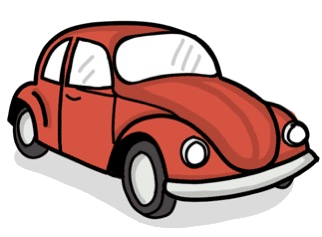
\includegraphics[width=0.7\linewidth]{icons/car.png} 
    & \textbf{Զգուշացե՛ք․} \textit{#1}%
    \end{tabular}%
    \bigskip 
    \par % ... and this too.
}

\newcommand{\hint}[1]{%
    \bigskip 
    \hspace{-0.14\textwidth}
    \noindent % I guess this is intended...
    \begin{tabular}{@{}m{0.13\textwidth}@{}m{\textwidth}@{}}%
    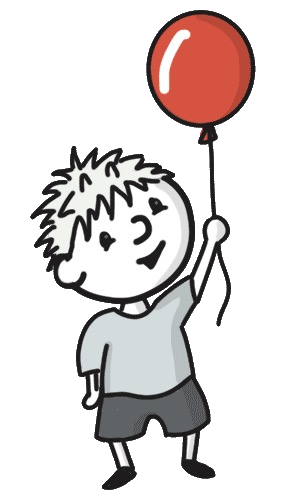
\includegraphics[width=0.7\linewidth]{icons/balloon.png} 
    & \textbf{Հուշում․} \textit{#1}%
    \end{tabular}%
    \bigskip 
    \par % ... and this too.
}

% \newcommand{\hint}[1]{%
%     \bigskip 
%     \hspace{-0.14\textwidth}
%     \noindent % I guess this is intended...
%     \begin{tabular}{@{}m{0.13\textwidth}@{}m{\textwidth}@{}}%
%     \HUGE  \WhiteKnightOnBlack
%     & \textbf{Հուշում․} \textit{#1}%
%     \end{tabular}%
%     \bigskip 
%     \par % ... and this too.
% }

% սլաքներ ու գույներ
\tikzset{>=latex} % for LaTeX arrow head
\usetikzlibrary{calc}
\usepackage[html]{xcolor}
\colorlet{veccol}{green!45!black}
\colorlet{myred}{red!90!black}
\colorlet{myblue}{blue!90!black}
\definecolor{ultramarine}{rgb}{0.22,0.93,0.62}
\colorlet{mypurple}{blue!50!red!80!black!80}
\colorlet{mygreen}{green!70!black}
\definecolor{myLavender}{HTML}{E5D7E4}
\definecolor{myLime}{HTML}{38eb9d}
\definecolor{myOrange}{HTML}{FAC17B}
\tikzstyle{vector}=[->,very thick,veccol]
\usetikzlibrary{arrows.meta}
\tikzstyle{thin arrow}=[dashed,thin,-{Latex[length=4,width=3]}]

% ընդգծված վերնագիր
\usepackage{soul}
\setul{0.45ex}{2pt}
\setulcolor{myLime}

% հայերեն enumerate
\makeatletter
\newcommand{\armenian}[1]{\expandafter\russian@realalph\csname c@#1\endcsname}

\def\russian@realalph#1{\ifcase#1\or
    a\or b\or g\or d\or e\or z\or \arme \or   u'\or \armto \fi}

\AddEnumerateCounter{\armenian}{\russian@realalph}
\makeatother

% side by side figures
\usepackage[demo]{graphicx}
\usepackage{subfig}
\usepackage{floatrow}

% զառեր
\newcommand{\dieimg}[1]{\raisebox{-0.2\height}{\includegraphics[width=0.5cm]{chapters/chapter 8/dice/#1.png}}}

% սիրտ հանելու խնդրի տրամագիրը
\newcommand\wideOne{3cm}
\newcommand\wideTwo{4cm}
\newcommand\wideThree{2.7cm}
\newcommand\wideFour{3cm}
\newcommand\distOne{2cm}
\newcommand\distTwo{1cm}


% խնդիրների համար
\newtheorem{problem}{Խնդիր}[chapter]

\newcommand{\va}{\mathbf{a}}
\newcommand{\vb}{\mathbf{b}}
\newcommand{\vc}{\mathbf{c}}
\newcommand{\vd}{\mathbf{d}}
\newcommand{\ve}{\mathbf{e}}
\renewcommand{\vv}{\mathbf{v}}
\newcommand{\vu}{\mathbf{u}}
\newcommand{\vw}{\mathbf{w}}
\newcommand{\vx}{\mathbf{x}}
\newcommand{\vy}{\mathbf{y}}
\newcommand{\vz}{\mathbf{z}}
\newcommand{\N}{\mathbb{N}}
\newcommand{\Z}{\mathbb{Z}}
\newcommand{\R}{\mathbb{R}}
\newcommand{\Q}{\mathbb{Q}}
\newcommand{\E}{\mathbb{E}}
\newcommand{\PP}{\mathbb{P}}
\newcommand{\F}{\mathcal{F}}
\newcommand{\rank}{\operatorname{rank}}
\newcommand{\Var}{\operatorname{Var}}
\newcommand{\Cov}{\operatorname{Cov}}

\usepackage{etoolbox}

% Patch the TOC line command to wrap Roman numerals in \textrm (not working)
% \makeatletter
% \renewcommand{\numberline}[1]{\hb@xt@\@tempdima{\rmfamily #1\hfil #1 aa}}
% \makeatother

% \usepackage{etoolbox}
% \makeatletter
% \pretocmd{\l@chapter}{\bgroup\renewcommand{\numberline}[1]{\hb@xt@\@tempdima{\rmfamily ##1\hfil}}}{}{}
% \apptocmd{\l@chapter}{\egroup}{}{}

% \pretocmd{\l@section}{\bgroup\renewcommand{\numberline}[1]{\hb@xt@\@tempdima{\rmfamily ##1\hfil}}}{}{}
% \apptocmd{\l@section}{\egroup}{}{}
% \makeatother




% \usepackage[bookmarksdepth=1]{hyperref}
% \usepackage[depth=0]{bookmark}

\begin{document}

%----------------------------------------------------------------------------------------
%	BOOK INFORMATION
%----------------------------------------------------------------------------------------

% \titlehead{The \texttt{kaobook} class}
% \subject{Use this document as a template}

\title[Շատ կարճ մաթեմատիկա]{Շատ կարճ մաթեմատիկա \\ մեքենայական ուսուցման համար}
% \subtitle{Customise this page according to your needs}

% \author[Federico Marotta]{Federico Marotta\thanks{A \LaTeX\ lover}}

\date{ }

% \publishers{An Awesome Publisher}

%----------------------------------------------------------------------------------------

\frontmatter % Denotes the start of the pre-document content, uses roman numerals
\def\thepage{\aroff {\roman{page}}} % makes the roman numerals out of armtex


%----------------------------------------------------------------------------------------
%	OPENING PAGE
%----------------------------------------------------------------------------------------

% \makeatletter
% \extratitle{
% 	% In the title page, the title is vspaced by 9.5\baselineskip
% 	\vspace*{9\baselineskip}
% 	\vspace*{\parskip}
% 	\begin{center}
% 		% In the title page, \huge is set after the komafont for title
% 		\usekomafont{title}\Huge\ul\@title
% 	\end{center}
% }
% \makeatother

\begin{titlepage}

	\raggedleft
 
	\vspace*{\baselineskip}
	
	\vspace*{0.167\textheight}
	
	\ul{\textbf{\Huge կարճ}}\\[\baselineskip] 
	\ul{\textbf{\Huge մաթեմ}}\\[\baselineskip] 
	\ul{\textbf{\Huge մեքենայական}}\\[\baselineskip] 
	\ul{\textbf{\Huge ուսուցման}}\\[\baselineskip] 
	\ul{\textbf{\Huge համար}}\\[\baselineskip] 

 \bigskip
 \bigskip
 \bigskip
 \bigskip
 \bigskip
 \bigskip
	
	{\Large \textit{համառոտ ձեռնարկ}}
	
	\vfill

\end{titlepage}



\chapter*{«Որքա՞ն մաթեմ է պետք {\bf ML}-ով զբաղվելու համար»}
\addcontentsline{toc}{chapter}{Ձեռնարկի մասին} % Add the preface to the table of contents as a chapter

Բավականին շատ։ 
Մեքենայական ուսուցումը ({\rm Machine Learning}-ը) ծավալուն գիտություն է, որով զբաղվելու համար առանցքային նշանակություն ունի իմանալ որոշ չափով մաթեմատիկա և ունենալ քթի ծակ։ 
Այս համառոտ ձեռնարկում հավաքված է {\rm ML}-ի համար անհրաժեշտ մաթեմի մի մասը՝ գրված շատ համառոտ ու ոչ խորը, նկարագրական ու ազատ ոճով։ Ընդամենը այնքան, որքանով հնարավոր է մի փոքր ինտուիցիա զարգացնել (ու եթե դուր գա, ապա հետագայում կարողանալ ինքնուրույն խորացնել գիտելիքները)։ 

\textbf{Սա դասագիրք չէ,} այլ պարզապես դասընթացի թրեյլեր։ Դասընթացի բուն նյութը սովորելու համար խոր\-հուրդ կտանք հետևյալ դասագրքերը․
\begin{itemize}
\item Գծային հանրահաշվից՝
\begin{itemize}
    \item[-] {\rm Poole, \textit{Linear Algebra}}
    \item[-] {\rm Johnston, \textit{Introduction to Linear and Matrix Algebra}}
    \item[-] {\rm Strang, \textit{Introduction to Linear Algebra}}
    \item[-] {\rm Boyd, Vandenberghe, \textit{Introduction to Applied Linear Algebra}}
\end{itemize}

\item Մաթեմատիկական անալիզից՝
\begin{itemize}
    \item[-] {\rm Stewart, \textit{Calculus}}
    \item[-] {\rm Hoffmann, Bradley, \textit{Calculus}}
    \item[-] {\rm Cummings, \textit{Real Analysis}}
    \item[-] {\rm Banner, \textit{The Calculus Lifesaver}}
    \item[-] Պողոսյան, \textit{Մաթեմատիկական անալիզ} (դասախոսություններ)
\end{itemize}

\item Հավանականությունների տեսությունից՝
\begin{itemize}
    \item[-] {\rm Ross, \textit{A First Course in Probability}}
    \item[-] {\rm Grimmett, Welsh, \textit{Probability}}
    \item[-] {\rm Blitzstein, Hwang, \textit{Introduction to Probability}}
\end{itemize}
\end{itemize}

Յուրաքանչյուր թեմա կարդալիս խորհուրդ կտանք պարտադիր անել երկու բան՝
\begin{enumerate}
    \item ամեն հարցի հասնելիս դադար տալ ու մտածել հարցի շուրջ 
\includegraphics[height=8*\fontcharht\font`\B]{icons/pancake.png} 
    \item թեման վերջացնելուց հետո կարդալ թեմայի շուրջ դասագրքի էջերն ու դիտել տեսանյութերը
\end{enumerate}

Խնդիրները լուծելիս, հարցերին պատասխանելիս կամ դասագրքում անծանոթ տերմիններ հանդիպելիս \linebreak դժվա\-րանալը կամ սխալվելը շատ նորմալ է, ընդհանրապես պետք չէ հուսահատվել։

Շնորհակալ կլինենք, եթե վրիպակներ գտնելու դեպքում գրեք \href{mailto:haykaprikyan@outlook.com}{այս հասցեով}։ Հետագայում մաթեմատի\-կա\-կան գիտելիքները խորացնելու համար խորհուրդ կտանք հետևյալ գրքերը՝
\begin{itemize}
\item {\rm Axler, \textit{Linear Algebra Done Right}}
\item {\rm Artin, \textit{Algebra}}
\item Մուսոյան, \textit{Մաթեմատիկական անալիզ} (մաս 1-2) 
\item {\rm Zorich, \textit{Mathematical Analysis} (vol. 1-2)}
\item {\rm Rudin, \textit{Principles of Mathematical Analysis}}\\ (նաև հայերեն՝ Ռուդին, \textit{Մաթեմատիկական անալիզի հիմունքները}) 
\item {\rm Durrett, \textit{Probability: Theory and Examples}} 
\end{itemize}
որոնք կարող եք գտնել \href{https://mathteam.notion.site}{\rm mathteam.notion.site} կայքում։



% \begin{flushright}
% \textit{Սխալների դեպքում խնդ}
% \end{flushright}

\index{preface}

%----------------------------------------------------------------------------------------
%	TABLE OF CONTENTS & LIST OF FIGURES/TABLES
%----------------------------------------------------------------------------------------

\begingroup % Local scope for the following commands

% Define the style for the TOC, LOF, and LOT
%\setstretch{1} % Uncomment to modify line spacing in the ToC
%\hypersetup{linkcolor=blue} % Uncomment to set the colour of links in the ToC
\setlength{\textheight}{230\hscale} % Manually adjust the height of the ToC pages

% Turn on compatibility mode for the etoc package
\etocstandarddisplaystyle % "toc display" as if etoc was not loaded
\etocstandardlines % "toc lines" as if etoc was not loaded

\tableofcontents % Output the table of contents

% \listoffigures % Output the list of figures

% Comment both of the following lines to have the LOF and the LOT on different pages
% \let\cleardoublepage\bigskip
% \let\clearpage\bigskip

% \listoftables % Output the list of tables

\endgroup

%----------------------------------------------------------------------------------------
%	MAIN BODY
%----------------------------------------------------------------------------------------

\mainmatter % Denotes the start of the main document content, resets page numbering and uses arabic numbers

% switch back to Arabic numerals
\def\thepage{\arabic{page}}


\setchapterstyle{kao} % Choose the default chapter heading style

\setchapterpreamble[u]{\margintoc}
\chapter{Վեկտորներ}
\labch{vectors}

\emergencystretch 2em

\section{Ներածություն}

Պատկերացրեք՝ ունեք $2$ հատ $10$ դրամանոց, $1$ հատ $20$ դրամանոց, $2$ հատ $50$ դրամանոց և $1$ հատ $200$ դրամանոց։ Ինչպե՞ս կարող ենք գրի առնել այդ փաստը։

Մի տարբերակ է՝ վերցնել ու աղյուսակով իրար տակ գրել յուրաքանչյուր մետաղադրամի արժեքը և մեր ունեցած քանակը․%\sidenote{Թեև $100$ դրամանոց չունենք, բայց ամեն դեպքում ավելացնենք նաև $100$-անոցի տողը․ միգուցե ինչ-որ պահի ունենանք։}
\begin{table}[h]
  % \centering
  \raggedright
  \begin{tabular}{|c|c|}
    \hline
    \textbf{արժեք} & \textbf{քանակ} \\
    \hline
    $10$ & $2$\\
    \hline
    $20$ & $1$\\
    \hline
    $50$ & $2$ \\
    \hline
    $100$ & $0$ \\
    \hline
    $200$ & $1$ \\
    \hline
  \end{tabular}
\end{table}

կամ, պարզապես, վերցնել այդ աղյուսակի երկու սյուները՝
\[
\begin{bmatrix}
10 \\ 20 \\ 50 \\ 100 \\ 200
\end{bmatrix}, \qquad \qquad \begin{bmatrix}
2 \\1 \\2 \\0 \\1 \\
\end{bmatrix}
\]

Վերևում գրված մի քանի թվերից բաղկացած օբյեկտներն անվանում ենք \textit{վեկտորներ։}

\begin{definition}
Իրական թվերի կարգավորված $n$-յակը\marginnote{կարգավորված $n$-յակ = ֆիքսված հեր\-թա\-կա\-նությամբ իրար կողք գրված $n$ հատ թիվ} կոչվում է \textbf{վեկտոր} (կամ \textbf{սյուն վեկտոր})՝
\[
\mathbf{v} = \begin{bmatrix} v_1 \\ v_2 \\ \vdots \\ v_n \end{bmatrix}
\]
իսկ \( v_1, v_2, \ldots, v_n \) թվերը կոչվում են վեկտորի \textbf{բաղադրիչներ}։
\end{definition}

Եթե նույն վեկտորը գրենք շրջած տեսքով՝ հորիզոնական, ապա կստանանք (ինչպես գուշակեցիք) \textit{տող վեկտոր՝}
\[\mathbf{v} = \begin{bmatrix} v_1 & v_2 & \ldots & v_n \end{bmatrix}։\]
$n$-չափանի բոլոր վեկտորների բազմությունը նշանակում ենք \( \mathbb{R}^n\)-ով։ Եթե նկատի ունենք, որ $\mathbf{v}$-ն \( \mathbb{R}^n \)-ից (այսինքն՝ $n$-չափանի) վեկտոր է, ապա գրում ենք՝ $\mathbf{v} \in \mathbb{R}^n$։

% \begin{exercise}
% Prove (or disprove) the Riemann hypothesis.
% \end{exercise}

Մասնավորապես, $\mathbb{R}^1$-ի վեկտորները հենց թվերն են՝ $[v]\in\mathbb{R}$:

\begin{example} 
Սրանք բոլորը համապատասխան չափանի վեկտորներ են՝
 \begin{align*}
    \mathbf{v}_1 &= \begin{bmatrix} 2 \\ -1 \\ 0 \end{bmatrix} \in \R^3 \\
    \mathbf{v}_2 &= \begin{bmatrix} 1 \\ 1 \\ 1 \\ 1 \end{bmatrix} \in \R^4 \\
    \mathbf{v}_3 &= \begin{bmatrix} -3 \\ 2 \end{bmatrix}\in \R^2 \\
    \mathbf{v}_4 &= \begin{bmatrix} 0 \\ 0 \\ 0 \end{bmatrix} \in \R^3 \\
    \mathbf{v}_5 &= \begin{bmatrix} 1 & -1 & 2 \end{bmatrix} \in \R^3
  \end{align*}
$\mathbf{v}_4$-ը կոչվում է $\R^3$ տարածության \textit{զրոյական վեկտոր} և նշանակվում թավ $0$-ով՝ $\mathbf{0}$։
\end{example}


 
\section{Գործողություններ վեկտորների հետ}

Նշանակենք 
\[
\mathbf{a} = \begin{bmatrix}
10 \\ 20 \\ 50 \\ 100 \\ 200
\end{bmatrix}, \qquad \mathbf{b} = \begin{bmatrix}
2 \\1 \\2 \\0 \\1 \\
\end{bmatrix}
\]
Այսպիսով՝
 $\mathbf{a}$, $\mathbf{b} \in \mathbb{R}^5$:
 
Պատկերացրեք՝ ինչ-որ մեկը մեզ տվեց, ասենք, $3 \times 100$ դրամ և ${1 \times 200}$ դրամ։ Նշանակենք
\[
\mathbf{c} = \begin{bmatrix}
0 \\ 0 \\ 0 \\ 3 \\ 1
\end{bmatrix}
\]
Այդ դեպքում կունենանք հետևյալ մետաղադրամները՝
\[
\mathbf{b} + \mathbf{c} = \begin{bmatrix}
2 \\1 \\2 \\0 \\1 \\
\end{bmatrix} + \begin{bmatrix}
0 \\ 0 \\ 0 \\ 3 \\ 1
\end{bmatrix} = \begin{bmatrix}
2+0 \\ 1+0 \\ 2+0 \\ 0+3 \\ 1+1
\end{bmatrix} = \begin{bmatrix}
2 \\ 1 \\ 2 \\ 3 \\ 2
\end{bmatrix}
\]

Ավելի ընդհանուր, 
\newpage 
\begin{definition}
Երկու $n$-չափանի  \( \mathbf{v} = \begin{bmatrix} v_1 \\ v_2 \\ \vdots \\ v_n \end{bmatrix} \) և \( \mathbf{u} = \begin{bmatrix} u_1 \\ u_2 \\ \vdots \\ u_n \end{bmatrix} \) 
\textbf{վեկտոր\-ների գումար} կանվանենք
  \begin{align*}
    \mathbf{v} + \mathbf{u} &= \begin{bmatrix} v_1 + u_1 \\ v_2 + u_2 \\ \vdots \\ v_n + u_n \end{bmatrix}
  \end{align*}
վեկտորը, այսինքն՝ գումարում ենք համապատասխան բաղա\-դրիչ\-ները։
\end{definition}

\warning{Տարբեր չափանի վեկտորներ իրար գումարել չենք կարող։}

Իսկ ի՞նչ, եթե ինչ-որ հրաշքով մետաղադրամները կրկնապատկվեին: Յուրաքանչյուր մետաղադրամից կունենայինք՝
$$2 \cdot \mathbf{b} = 2\cdot \begin{bmatrix}
2 \\1 \\2 \\0 \\1 \\
\end{bmatrix} = \begin{bmatrix}
4 \\2 \\4 \\0 \\2 \\
\end{bmatrix} $$
հատ։ Ուրեմն սահմանենք՝ 
\begin{definition}
Ցանկացած \( \mathbf{v} = \begin{bmatrix} v_1 \\ v_2 \\ \vdots \\ v_n \end{bmatrix} \) վեկտորի և  $c\in\R$ թվի\marginnote{թիվ բառի փոխարեն կօգտագործենք նաև \textit{սկալյար} {\it (scalar)} բառը} համար \textbf{$\mathbf{v}$ վեկտորի բազմապատկում $c$ թվով} կանվանենք
  \begin{align*}
    c \cdot \mathbf{v} &= \begin{bmatrix} c \cdot v_1 \\ c \cdot v_2 \\ \vdots \\ c \cdot v_n \end{bmatrix}
  \end{align*}
վեկտորը, այսինքն՝ $\mathbf{v}$-ի բոլոր բաղադրիչները բազմապատկում ենք $c$-ով։
\end{definition}

Ինչպես թվերի գումարում-բազմապատկումը, այնպես էլ վեկտորների գումարման և թվով բազմապատկման գործողությունները օժտված են հետևյալ լավ հատկություններով՝
\begin{itemize}
    \item զուգորդականություն, այսինքն՝
    \[
      (\mathbf{u} + \mathbf{v}) + \mathbf{w} = \mathbf{u} + (\mathbf{v} + \mathbf{w}) \quad  \text{ և } \quad
     (c \cdot d) \cdot \mathbf{v} = c \cdot (d \cdot \mathbf{v})
    \]

    \item տեղափոխականություն, այսինքն՝
        \[
     \mathbf{u} + \mathbf{v} = \mathbf{v} + \mathbf{u} \quad  \text{ և } \quad
     c \cdot (d \cdot \mathbf{v}) =  d \cdot (c \cdot \mathbf{v}) = (cd) \cdot \mathbf{v}
    \]

    \item բաշխականություն, այսինքն՝
    \[
     c \cdot (\mathbf{v} + \mathbf{u}) = c \cdot \mathbf{v} + c \cdot \mathbf{u}
    \]
\end{itemize}
ցանկացած  $\mathbf{u}$, $\mathbf{v} \in  \mathbb{R}^n$ վեկտորների և $c$, $d\in \R$ թվերի համար։

Վերջապես պատկերացրեք, որ մտնում եք խանութ և ծախսում ${2 \times 50}$ դրամանոց։ Ինչպե՞ս կփոխվի Ձեր գրպանի պարունակությունը։

\begin{definition}
Ցանկացած \( \mathbf{v} = \begin{bmatrix} v_1 \\ v_2 \\ \vdots \\ v_n \end{bmatrix} \) վեկտորի \textbf{հակադիր} կանվանենք
  \begin{align*}
     -\mathbf{v} &= \begin{bmatrix} -v_1 \\ -v_2 \\ \vdots \\ -v_n \end{bmatrix}
  \end{align*}
վեկտորը, այսինքն՝ $\mathbf{v}$ բոլոր բաղադրիչները բազմապատկում ենք $-1$-ով։
\end{definition}

Իսկ հակադիրի միջոցով սահմանենք վեկտորների հանումը՝
\begin{definition}
Երկու $n$-չափանի  \( \mathbf{u} = \begin{bmatrix} u_1 \\ u_2 \\ \vdots \\ u_n \end{bmatrix} \) և  \( \mathbf{v} = \begin{bmatrix} v_1 \\ v_2 \\ \vdots \\ v_n \end{bmatrix} \) 
\textbf{վեկտոր\-ների տարբերություն} կանվանենք $\vu$-ի և $-\mathbf{v}$-ի գումարը՝
  \begin{align*}
    \mathbf{v} + \mathbf{u} &= \begin{bmatrix} v_1 + u_1 \\ v_2 + u_2 \\ \vdots \\ v_n + u_n \end{bmatrix}
  \end{align*}
այսինքն՝ հանում ենք համապատասխան բաղադրիչները։
\end{definition}

\warning{Տարբեր չափանի վեկտորներ իրարից հանել չենք կարող։}

\begin{example}
    \[
    \begin{bmatrix} 2 \\ -1 \\ 3 \end{bmatrix} - \begin{bmatrix} 1 \\ 4 \\ 0 \end{bmatrix} = \begin{bmatrix} 2 - 1 \\ -1 - 4 \\ 3 - 0 \end{bmatrix} = \begin{bmatrix} 1 \\ -5 \\ 3 \end{bmatrix}
    \]
\end{example}


\section{Վեկտորների շրջումը}

Երբեմն ունենում ենք, ենթադրենք, $\mathbf{v}=\begin{bmatrix}
    3 \\ 4
\end{bmatrix}$ վեկտորը և ցանկանում ենք ինչ-որ ձևով նշանակել $\begin{bmatrix}
    3 & 4
\end{bmatrix}$ վեկտորը, այսինքն՝ որպես սյուն գրված վեկտորը գրել որպես տող։ Այդ դեպքում կգրենք պարզապես, որ
\[
\mathbf{v}^T = \begin{bmatrix}
    3 \\ 4
\end{bmatrix}^T = \begin{bmatrix}
    3 & 4
\end{bmatrix}
\]

\begin{definition}
\( \mathbf{v} = \begin{bmatrix} v_1 \\ v_2 \\ \vdots \\ v_n \end{bmatrix} \) սյուն \textbf{վեկտորի տրանսպոնացված} (կամ \textbf{շրջած}) ենք անվանում
\begin{align*}
\mathbf{v}^T = \begin{bmatrix} v_1 & v_2 & \cdots & v_n \end{bmatrix}
\end{align*}
տող վեկտորը, այսինքն՝ նույն $\mathbf{v}$-ն, բայց շրջած։
\end{definition}
Նույն ձևով սահմանում ենք տող վեկտորի տրանսպոնացվածը՝ որպես համապատասխան սյուն վեկտոր։ 

\begin{example}
 \[
    \begin{bmatrix} 2 \\ -1 \\ 3 \end{bmatrix}^T = \begin{bmatrix} 2 & -1 & 3 \end{bmatrix}
    \]
    \[
    \begin{bmatrix} 1 & 0 & -2 \end{bmatrix}^T = \begin{bmatrix} 1 \\ 0 \\ -2 \end{bmatrix}
    \]
\end{example}

Նկատենք, որ ցանկացած $c$ թվի և $\mathbf{v}$ վեկտորի համար 
\[
(c \cdot \mathbf{v})^T = c \cdot \mathbf{v}^T 
\]

\question{Ի՞նչ եք կարծում, ինչի՞ է հավասար $(\mathbf{v}^T)^T $-ն։}

Ինչպես տեսնում եք, տող և սյուն վեկտորների միջև էական տարբե\-րու\-թյուն չկա․ գրելաձևը տարբեր է, բայց բովանդակությունը՝ թվերը նույնն են։ Այնպես որ այսուհետև վեկտորների մասին խոսելիս չենք նշի «տող վեկտոր» կամ «սյուն վեկտոր», այլ պարզապես կասենք «վեկտոր»։

\warning{Տող վեկտորին սյուն վեկտոր գումարել չի կարելի:}


\section{Սկալյար արտադրյալ}

Վերադառնանք մեր մետաղադրամներին։ Ունեինք $\mathbf{a} = \begin{bmatrix}
10 \\ 20 \\ 50 \\ 100 \\ 200
\end{bmatrix}$  արժո\-ղու\-թյամբ  $\mathbf{b} = \begin{bmatrix}
2 \\1 \\2 \\0 \\1 \\
\end{bmatrix}$ քանակով մետաղադրամներ։

\question{Որքա՞ն գումար ունենք ընդհանուր։}

\begin{definition}
\( \mathbf{u} = \begin{bmatrix} u_1 \\ u_2 \\ \vdots \\ u_n \end{bmatrix} \) և \( \mathbf{v} = \begin{bmatrix} v_1 \\ v_2 \\ \vdots \\ v_n \end{bmatrix} \) վեկտորների \textbf{սկալյար արտադրյալ} կանվանենք
\[
\mathbf{u} \cdot \mathbf{v} = u_1 \cdot v_1 + u_2 \cdot v_2 + \cdots + u_n \cdot v_n
\]
թիվը։
\end{definition}
\begin{example}
Եթե  \( \mathbf{u} = \begin{bmatrix} 2 \\ -1 \\ 3 \end{bmatrix} \) և \( \mathbf{v} = \begin{bmatrix} 1 \\ 4 \\ 0 \end{bmatrix} \), ապա
    \[
    \mathbf{u} \cdot \mathbf{v} = (2 \cdot 1) + (-1 \cdot 4) + (3 \cdot 0) = 2 - 4 + 0 = -2
    \]
\end{example}

Մեր ունեցած գումարը պարզելու համար կարող ենք հաշվել արժո\-ղու\-թյուն\-ների ու քանակների  $\mathbf{a}$ և $ \mathbf{b}$ վեկտորների սկալյար արտադրյալը՝
$$\mathbf{a} \cdot \mathbf{b}= \begin{bmatrix}
2 \\1 \\2 \\0 \\1 \\
\end{bmatrix}\cdot \begin{bmatrix}
10 \\ 20 \\ 50 \\ 100 \\ 200
\end{bmatrix} = 2 \cdot 10 + 1 \cdot 20 + 2 \cdot 50 + 0 \cdot 100 + 1\cdot 200 = 340 $$

Նկատենք, որ եթե երկու վեկտորների գումարը կամ տարբերությունը վեկտոր է, ապա դրանց սկալյար արտադրյալը \textit{թիվ է} (ինչի համար էլ կոչվում է \textit{սկալյար} արտադրյալ)։ Իսկ քանի որ սկալյար արտադրյալը նշանակում են կետիկով՝ $\va \cdot \vb$, անգլերենում այն կոչվում է նաև {\it dot product:}

\warning{Սկալյար արտադրյալը սահմանված է միայն նույն չափանի վեկտորների համար։}

Ինչպես գումարման և թվով բազմապատկման դեպքում, սկալյար արտադրյալը ևս օժտված է օգտակար հատկություններով․
\begin{itemize}
  \item տեղափոխականություն՝ $$ \mathbf{u} \cdot \mathbf{v} = \mathbf{v} \cdot \mathbf{u}$$
  \item զուգորդականություն՝ $$(c \cdot \mathbf{u}) \cdot \mathbf{v} = c \cdot (\mathbf{u} \cdot \mathbf{v}) = \mathbf{u} \cdot (c \cdot \mathbf{v})$$
  \item բաշխականություն՝ $$ (\mathbf{u} + \mathbf{v}) \cdot \mathbf{w} = \mathbf{u} \cdot \mathbf{w} + \mathbf{v} \cdot \mathbf{w} $$
  \item դրական որոշյալություն՝ 
  $$\mathbf{u} \cdot \mathbf{u} \geq 0, $$
  ընդ որում զրոյի հավասարվելու միակ դեպքն այն է, երբ $\mathbf{u} = \mathbf{0}$:
\end{itemize}

\question{Ինչո՞ւ է չորրորդ հատկությունը ճիշտ ցանկացած վեկտորի համար։}


\begin{example}
Հաշվենք \( (5\mathbf{u} - \mathbf{v}) \cdot \mathbf{w} \) արտահայտության արժեքը
 \[ \mathbf{u} = \begin{bmatrix} 1 \\ -2 \\ 3 \end{bmatrix}, \qquad  \mathbf{v} = \begin{bmatrix} 0 \\ 4 \\ -1 \end{bmatrix}, \qquad \mathbf{w} = \begin{bmatrix} -2 \\ 1 \\ 2 \end{bmatrix} \]
 վեկտորների համար։

  \begin{align*}
      (5\mathbf{u} - \mathbf{v}) \cdot \mathbf{w} &= \left(5\cdot\begin{bmatrix} 1 \\ -2 \\ 3 \end{bmatrix} - \begin{bmatrix} 0 \\ 4 \\ -1 \end{bmatrix}\right) \cdot \begin{bmatrix} -2 \\ 1 \\ 2 \end{bmatrix} \\&= \left(\begin{bmatrix} 5 \\ -10 \\ 15 \end{bmatrix} - \begin{bmatrix} 0 \\ 4 \\ -1 \end{bmatrix}\right) \cdot \begin{bmatrix} -2 \\ 1 \\ 2 \end{bmatrix} 
      \\&= \begin{bmatrix} 5 \\ -14 \\ 16 \end{bmatrix} \cdot \begin{bmatrix} -2 \\ 1 \\ 2 \end{bmatrix} = 5 \cdot (-2) + (-14) \cdot 1 + 16 \cdot 2 = 8  \end{align*}
\end{example}

% \question{Իմաստ ունի՞ $u$։}


\section{Վեկտորների պատկերումը երկրաչափորեն}

Մինչ այս պահը վեկտորները մեր համար զուտ ինչ-որ թվացուցակներ են։ Պարզվում է, որ իրականում վեկտորներն ունեն շատ գեղեցիկ երկրաչափական մեկնաբանություն։ 

Վերցնենք օրինակ՝
\[
\vv=\begin{bmatrix}2\\3    \end{bmatrix}
\]
երկչափ վեկտորը։ Այն կարող ենք պատկերել հետևյալ ձևով․ վերցնենք կոորդինատական հարթության $(0, 0)$ սկզբնակետը և սլաքով միացնենք $(2, 3)$ կոորդինատներով կետին։

\begin{center}
  \begin{tikzpicture}[scale=1]
    \draw[->] (0,0) -- (2,3) node[midway, above left] {$\mathbf{v}$};
    \draw[dashed] (0,0) -- (2,0) node[midway, below] {$2$};
    \draw[dashed] (2,0) -- (2,3) node[midway, right] {$3$};
  \end{tikzpicture}
\end{center}

Արդյունքում կստանանք սլաք (կամ ուղղորդված հատված), որը հենց կլինի $\vv$ վեկտորի երկրաչափական պատկերը։ Այս եղանակով կարող ենք $\R^2$ տարածության բոլոր վեկտորների մասին մտածել որպես $(0, 0)$ կետից սկսվող որոշակի ուղղություն և երկարություն ունեցող \textit{սլաքների՝}
\[
\begin{bmatrix}
    x \\ y
\end{bmatrix} \quad \mapsto \quad (0,0)\text{-ից սկսվող սլաք դեպի }(x, y)
\]

Նման ձևով $\R^3$-ի վեկտորները նույնպես կարող ենք պատկերել որպես եռաչափ ({\rm 3D}) տարածության մեջ սլաքներ։ Ինչպես ընթացքում կտեսնենք, վեկտորներին առնչվող բազմաթիվ գաղափարներ բավարար է հասկանալ ընդամենը $2$-չափ ու $3$-չափ դեպքերում,\marginnote{2-3 բաժակ հետո հնարավոր է պատկե\-րել նաև $\R^4$-ի վեկտորները} որպեսզի պատկե\-րաց\-նենք, թե ինչ է տեղի ունենում ավելի մեծ չափանի տարածու\-թյուն\-նե\-րում։

Վեկտորները երկրաչափորեն պատկերելը օգտակար է հատկապես նրանով, որ այսպես ավելի հեշտ է պատկերացնել դրանց հետ կատարվող գործողությունները․

\begin{description}
\item[Գումարում․] Երկու $\mathbf{u}$ և $\mathbf{v}$ վեկտորներ գումարելու համար $\vv$ վեկտորի սկզբնակետը տեղադրում ենք $\vu$ վեկտորի վերջնակետից։ Արդյուն\-քում $\vu$-ի սկզբնակետից դեպի $\vv$-ի վերջնակետը ուղղված վեկտորը կլինի $\mathbf{u} + \mathbf{v}$-ն։

\begin{center}
  \begin{tikzpicture}[scale=0.8]
    \draw[->] (0,0) -- (2,3) node[midway, above left] {$\mathbf{u}$};
    \draw[->] (2,3) -- (5,1) node[midway, above right] {$\mathbf{v}$};
    \draw[->,myred] (0,0) -- (5,1) node[midway, below] {$\mathbf{u} + \mathbf{v}$};
  \end{tikzpicture}
\end{center}

\item[Հակադիր․] $\mathbf{v}$ վեկտորի $-\mathbf{v}$ հակադիրը այն վեկտորն է, որն ունի նույն երկարությունը և ուղղված է $\vv$-ին հակառակ։

    \begin{center}
      \begin{tikzpicture}[scale=0.8]
        \draw[->] (0,0) -- (3,2) node[midway, above left] {$\mathbf{v}$};
        \draw[->,myred] (0,0) -- (-3,-2) node[midway, below] {$\qquad -\mathbf{v}$};
      \end{tikzpicture}
    \end{center}

\item[Հանում․] $\mathbf{u}$ վեկտորից $\mathbf{v}$ վեկտորը հանելու համար կարող ենք $\vu$-ին գումարել $\vv$-ի հակադիրը, կամ ուրիշ կերպով՝ $\vu$-ն ու $\vv$-ն պատկերել միևնույն սկզբնակետից, ծայրակետերը միացնել իրար՝ ստանալով եռանկյուն, և վերցնել $\vv$-ի վերջնակետից դեպի $\vu$-ի վերջնակետն ուղղված վեկտորը։

\begin{center}
  \begin{tikzpicture}[scale=0.8]
    \draw[->] (0,0) -- (2,3) node[midway, right] {$\;\mathbf{u}$};
    \draw[->] (0, 0) -- (-3,2) node[midway, left] {$\mathbf{v}\quad $};
    \draw[->,myred] (-3,2) -- (2,3) node[midway, above] {$\mathbf{u} - \mathbf{v}$};
  \end{tikzpicture}
\end{center}


\item[Թվով բազմապատկում․] $\mathbf{v}$ վեկտորը $c$ դրական թվով բազմապատկելիս այն ձգվում/սեղմվում է $c$ անգամ, այսինքն՝ ստացվում է նույն ուղղությամբ, բայց տարբեր երկարությամբ վեկտոր։

\begin{center}
  \begin{tikzpicture}[scale=0.8]
    \draw[->] (0,0) -- (3,2) node[midway, above left] {$\mathbf{v}$};
    \draw[->,myred] (0,0) -- (6,4) node[near end, above left] {$2  \mathbf{v}$};
  \end{tikzpicture}
\end{center}

Բացասական $c$-ով բազմապատկելիս երկարությունը կրկին բազմապատկվում է $|c|$ անգամ, բայց վեկտորը շրջվում է հակառակ ուղղությամբ։
\end{description}


\question{Ի՞նչ է դառնում վեկտորը, երբ այն բազմապատկում ենք $0$-ով։}


\begin{example}
Եթե $\va = \begin{bmatrix} 3 & 2 \end{bmatrix}$ և $\vb = \begin{bmatrix} 2 & 0 \end{bmatrix}$, ապա $3\va+\vb$-ն գտնելու համար պետք է
\begin{enumerate}
    \item $\va$-ն ձգել $3$ անգամ,
    \item $\vb$-ն տեղադրել ստացված $3\va$ վեկտորի վերջնակետից,
    \item (լրացրու ինքդ)
\end{enumerate}

\begin{center}
\begin{tikzpicture}[scale=0.8]
  \draw[->] (0,0) -- (3,2) node[midway, above left] {$\mathbf{a}$};
  \draw[->] (0,0) -- (2,0) node[midway, below] {$\mathbf{b}$};
  \draw[->] (0,0) -- (9,6) node[midway, left] {$3\mathbf{a}\;\;\;$};
  \draw[->] (9,6) -- (11,6) node[midway, above] {$\mathbf{b}$};
  \draw[->,myred] (0,0) -- (11,6) node[midway, below] {\;\;\;\;\;\;\;\;$3\mathbf{a} + \mathbf{b}$};
\end{tikzpicture}
\end{center}
\end{example}

\section{Նորմ}

Վեկտորների երկրաչափական պատկերումից հարց է առաջանում․ եթե վեկտորը սլաք է, ապա ինչի՞ է հավասար նրա երկարությունը։ 
Դե, հատվածի երկարությունը նրա սկզբնակետի և վերջնակետի միջև եղած հեռավորությունն է։ Իսկ ինչպե՞ս հաշվենք այդ հեռավորությունը, օրինակ, $\begin{bmatrix}
    3 & 4
\end{bmatrix}$ վեկտորի դեպքում՝ օգտվելով դրա կոորդինատներից ($3$ և $4$ թվերից)։ 


\begin{figure}[h]
    \centering
    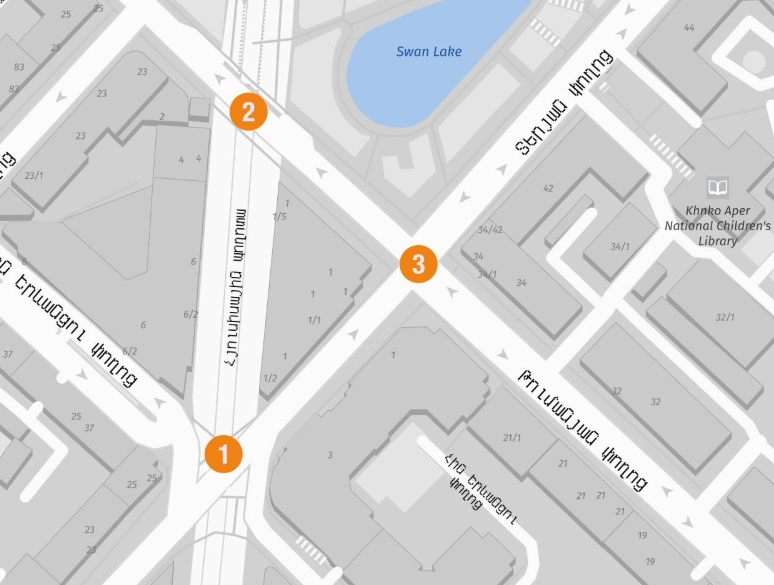
\includegraphics[width=0.75\linewidth]{chapters/chapter 1/evn_map.png}
\end{figure}

Որքա՞ն ճանապարհ պետք է անցնել, օրինակ, Հյուսիսային-Տերյան \circled{$1$} և Հյուսիսային-Թումանյան \circled{$2$} խաչմերուկների միջև։ 

\textbf{Հետիոտնի տեսանկյունից՝} \circled{$1$} և \circled{$2$} կետերի հեռավորությունը հավասար է դրանք միացնող հատվածի երկարությանը։

\textbf{Վարորդի տեսանկյունից՝} \circled{$1$}-\circled{$2$} հատվածի երկարությունը որևէ իմաստ չունի։ Փոխարենը հեռավորությունը հաշվելու համար պետք է \circled{$1$}-\circled{$3$} հատվածի երկարությանը գումարել \circled{$2$}-\circled{$3$}-ի երկարությունը։



Ուրեմն կախված իրավիճակից՝ հեռավորություն և վեկտորի երկարու\-թյուն գաղափարները կարող ենք տարբեր կերպ սահմանել։ Պայ\-մա\-նա\-վորվենք այսուհետ «երկարություն» բառի փոխարեն ասել վեկտորի \textit{նորմ։}

\begin{definition}
$\mathbf{v} = \begin{bmatrix} v_1 \\ v_2 \\ \dots \\ v_n \end{bmatrix}$ վեկտորի \textbf{մանհեթընյան նորմ} (կամ $\operatorname{L}_1$ նորմ) կանվանենք
\[ \|\mathbf{v}\|_1 = |v_1| + |v_2| + \dots + |v_n| \]
թիվը, այսինքն՝ նրա բաղադրիչների մոդուլների գումարը։
\end{definition}

\begin{example}
$\mathbf{v} = \begin{bmatrix} 3 & 4 \end{bmatrix}$ վեկտորի մանհեթընյան նորմը կլինի՝
\[ \|\mathbf{v}\|_1 = |3| + |4| = 7 \]
\end{example}

\newpage 

\begin{definition}
$\mathbf{v} = \begin{bmatrix} v_1 \\ v_2 \\ \dots \\ v_n \end{bmatrix}$ վեկտորի \textbf{էվկլիդյան նորմ} (կամ $\operatorname{L}_2$ նորմ) կանվանենք
\[ \|\mathbf{v}\|_2 = \sqrt{v_1^2 +v_2^2+\dots+ v_n^2}\marginnote{նկատենք, որ $\|\vv\|_2 = \sqrt{\vv \cdot \vv}$} \]
թիվը, այսինքն՝ նրա բաղադրիչների քառակուսիների գումարի արմատը։
\end{definition}

\begin{example}
$\mathbf{v} = \begin{bmatrix} 3 & 4 \end{bmatrix}$ վեկտորի էվկլիդյան նորմը կլինի՝
\[ \|\mathbf{v}\|_2 = \sqrt{3^2 + 4^2} = 5 \]
\end{example}

Վեկտորի էվկլիդյան նորմը դպրոցական երկրաչափությունից մեզ հայտնի ստանդարտ երկարությունն է։ Հաճախ ինդեքսում գրվող փոքրիկ $2$-ը բաց ենք թողում և $\|\mathbf{v}\|_2$-ի փոխարեն գրում $\|\mathbf{v}\|$։


Կան վեկտորների բազմաթիվ այլ նորմեր (երկարությունը հաշվելու եղանակներ), բայց հետագայի համար մեզ այս երկուսը բավարար են։ Նշենք, որ անկախ նրանից, թե ինչպես կսահմանենք վեկտորի նորմը, այն բավարարում է հետևյալ երեք պայմաններին՝ 
\begin{enumerate}
    \item $\|\vv\|\ge 0$, ընդ որում զրոյի հավասար է այն և միայն այն դեպքում, եթե $\vv=\mathbf{0}$,\marginnote{\textit{«գծենք $-3$ երկարությամբ վեկտոր»՝} այնքան էլ չի հնչում}
    \item $\|c\vv\| = |c|\cdot \|\vv\|$,
    \item $\|\vv+\vu\| \le \|\vv\|+\|\vu\|$։

    \begin{figure}[h]
    \centering
\begin{tikzpicture}[line cap=round]
  \coordinate (O) at (0,0);
  \coordinate (A) at ( -3:2.1);
  \coordinate (B) at ( 55:1.4);
  \coordinate (A+B) at ($(A)+(B)$);
  
  \draw[vector,thin arrow,myred!40] (B) -- (A+B) node[midway,above] {$\vv$};
  \draw[vector,thin arrow,myblue!40] (A) -- (A+B) node[midway,below right=0.08] {$\vu$};
  
  \draw[vector,myred] (O) -- (A) node[midway,below] {$\vv$};
  \draw[vector,myblue] (O) -- (B) node[midway,above left=0.08] {$\vu$};
  \draw[vector,mypurple] (O) -- (A+B) node[above right=0.1] {$\vv+\vu$};
\end{tikzpicture}
\end{figure}
\end{enumerate}

Վերջին հատկությունը կոչվում է \textit{եռանկյան անհավասարություն} (ի՞նչ եք կարծում, ինչո՞ւ)։ 


\section{Անկյուն}

Վերջապես, եթե վեկտորը երկրաչափորեն պարզապես ինչ-որ սլաք է, իսկ սլաքը բնութագրվում է երկու մեծությամբ՝ երկարություն և ուղղություն, ապա նորմից բացի պետք է գոյություն ունենա նաև մեկ այլ գործիք/միջոց, որով հնարավոր կլինի նկարագրել ուղղությունները։ Այդ գործիքը \textit{անկյունն} է։



\begin{center}
\begin{tikzpicture}
\coordinate (O) at (0,0);
\coordinate (U) at (2,2);
\coordinate (V) at (4,1);

\draw[->,thick] (O) -- (U) node[midway, left] {$\mathbf{u}\;\;$};
\draw[->,thick] (O) -- (V) node[midway, below] {$\;\mathbf{v}$};
\draw[myblue] (1, 0.27) arc[start angle=30, end angle=60, radius=1, "$\theta$"];
\end{tikzpicture}\marginnote{հիշո՞ւմ եք դպրոցական երկրաչափու\-թյունից հայտնի բանաձևը՝
\[
\va \cdot \vb = \|\va\| \|\vb\| \cos\alpha,
\]
որտեղ $\alpha$-ն $\va$ և $\vb$-ի կազմած անկյունն է}
\end{center}

Սահմանենք երկու վեկտորների կազմած անկյան գաղափարը հետևյալ կերպ․

\begin{definition}
$\vu$ և $\vv$ \textbf{վեկտորների կազմած անկյուն} կանվանենք այն $\theta$ անկյունը ($0 \le \theta \le \pi$), որի համար
\[ \cos \theta = \frac{\mathbf{u} \cdot \mathbf{v}}{\|\mathbf{u}\| \cdot \|\mathbf{v}\|} \]
\end{definition}

\begin{example}
Գտնենք $\mathbf{u} = \begin{bmatrix} 3 & 4 \end{bmatrix}$ և $\mathbf{v} = \begin{bmatrix} 7 & 1 \end{bmatrix}$ վեկտորների կազմած անկյունը։ 
\[ \cos \theta = \frac{\mathbf{u} \cdot \mathbf{v}}{\|\mathbf{u}\| \cdot \|\mathbf{v}\|}  = \frac{(3 \cdot 7) + (4 \cdot 1)}{\sqrt{3^2 + 4^2} \cdot \sqrt{7^2 + 1^2}} = \frac{25}{\sqrt{25} \cdot \sqrt{50}} =\frac{1}{\sqrt{2}}\]
\[ \frac{1}{\sqrt{2}}=\cos{\frac{\pi}{4}} \quad \Rightarrow \quad \theta = \arccos \frac{1}{\sqrt{2}} = \frac{\pi}{4}=45^\circ \]
\end{example}

Փաստորեն, վեկտորների կազմած անկյունը սահմանեցինք այնպես, որ
\[ \vv \cdot \vu  = \|\vv\| \cdot \|\vu\| \cdot \cos{\theta}։\]

\question{Երկրաչափորեն ի՞նչ է ցույց տալիս վեկտորների սկալյար արտադրյալը։}
% \hint{Պրոյեկցիա։}

Վեկտորների կազմած անկյանը նայելով՝ կարելի է եզրակացնել, թե որքանով են վեկտորները իրար նման կամ իրարից տարբեր։ Իրոք, եթե երկու վեկտորներ ուղղված են իրար մոտ ուղղություններով, ապա նրանց կազմած անկյունը փոքր է: Եթե դրանք ուղղված են միմյանց գրեթե հակառակ, ապա կազմած անկյունը մոտ է $180^\circ$-ի։ Մասնավորապես՝ ցանկացած $\vv \in  \mathbb{R}^n$ վեկտոր ինքն իր հետ կազմում է  $0^\circ$ անկյուն, իր հակադիրի հետ՝ $180^\circ$ անկյուն։

Իսկ եթե վեկտորներն ուղղված են ոչ նույն, ոչ էլ հակառակ, այլ իրար հետ կապ չունեցող ուղղություններով (ասենք՝ մեկը վերև, մյուսը՝ աջ), ապա դրանց կազմած անկյունը կլինի $\theta \approx 90^\circ = \frac{\pi}{2}$։ Հետևաբար ${\cos \theta = 0}$, ուրեմն $\vv \cdot \vu = 0$։ Այսպիսով ստացանք, որ եթե երկու վեկտորներ ուղղահայաց են, ապա նրանց \textbf{սկալյար արտադրյալը զրո է։}

Սա այս գլխի ամենակարևոր արդյունքներից է․ եթե $\vu \cdot \vv \approx 0$, ապա $\vu$ և $\vv$ վեկտորներն ուղղված են միմյանց (մոտավորապես) ուղղահայաց, այսինքն՝ իրար հետ կապ չունեցող ուղղություններով։

\bigskip 

\begin{theory}
.
\begin{itemize}
\item կարդալ [{\rm Poole}], 2-12 էջերը (վեկտորներ) 
\item կարդալ [{\rm Johnston}], 10-14 (նորմ), 16-19 (անկյուն) էջերը  
\item դիտել  {\rm 3b1b}-ի \href{https://www.3blue1brown.com/lessons/vectors}{1-ին տեսադասը} գծային հանրահաշվից (նաև՝ \href{https://youtu.be/7-r7Z2iH0Ps}{հայերեն}) 
\end{itemize}
\end{theory}

\newpage

\section{Խնդիրներ}


\begin{problem}
Տրված են հետևյալ վեկտորները՝
\[
\va= \begin{bmatrix} 3 \\ -1 \\ 2 \end{bmatrix}, \qquad \vb=\begin{bmatrix} 2 \\ 4 \\ -5 \end{bmatrix}, \qquad \vc = \begin{bmatrix}
    5 \\ 6.5 \\ -7
\end{bmatrix}
\]

Գտեք արտահայտության արժեքը․
\begin{enumerate}[label={\alph*}․]
\item $\va+\vb$
\item $\va+\vb-\vc$
\item $\va^T+\vb^T-\vc^T$
\item $3\va^T+4\vb^T-2\vc^T$
\item $6\va^T+8\vb^T-4\vc^T$
\item $\va \cdot \vb$
\item $(3\va - 6\vb) \cdot \vc$
\item $\va \cdot (4\va^T - \vb^T)^T$
\end{enumerate}
\end{problem}

\begin{problem}
Թարգմանչական գրասենյակը թարգմանեց 
\[\va=\begin{bmatrix}
    24 & 17 & 9 & 13
\end{bmatrix}\]
փաստաթուղթ համապատասխանաբար անգլերեն, ֆրանսերեն, գերմա\-նե\-րեն և ռուսերեն։ Յուրաքանչյուր լեզվի համար մեկ էջ թարգմանելը տևում է մոտավորապես $\vb=\begin{bmatrix}
    5 & 10 & 11 & 7
\end{bmatrix}$ րոպե։ 

Ընդհանուր որքա՞ն ժամանակ պահանջվեց փաստաթղթերը թարգմա\-նե\-լու համար։ Միջինում քանի՞ րոպե ծախսեց թարգմանիչներից յուրա\-քանչ\-յուրը, եթե գրասենյակում կա $4$ թարգմանիչ։ Պատասխանը արտահայտեք $\va$-ով և $\vb$-ով։
\end{problem}

\begin{problem}
Հաշվեք հետևյալ վեկտորների մանհեթընյան և էվկլիդյան նորմերը․

\begin{enumerate}[label={\alph*}․]
\item $\va= \begin{bmatrix} 2\\-9\\3 \end{bmatrix}$

\item $\va-2\vb$, որտեղ $\va= \begin{bmatrix}3\\4\\1\\0\end{bmatrix},\  \vb = \begin{bmatrix}4\\5\\-2\\-1\end{bmatrix}$

\item $-3\vc$, որտեղ $\vc= \begin{bmatrix}2\\-5\\6\end{bmatrix}$
\end{enumerate}
\end{problem}

\begin{problem}
Որքա՞ն անկյուն են կազմում
\begin{enumerate}[label={\alph*}․]
\item $\va= \begin{bmatrix} 2\\1\\1\end{bmatrix}$ և $\vb= \begin{bmatrix} 1\\-3\\3\end{bmatrix}$ վեկտորները

\item նախորդ խնդրի $\va$ ու $\vc$ վեկտորները
\end{enumerate}
\end{problem}


\begin{problem}
Ամենաշատը քանի՞ վեկտոր կարող ենք տեղադրել $\R^2$ հարթության մեջ, որպեսզի ցանկացած երկուսի սկալյար արտադրյալը լինի դրական։ Իսկ որպեսզի լինի բացասակա՞ն։
\end{problem}

\setchapterpreamble[u]{\margintoc}
\chapter{Գծային ձևափոխություններ}
\labch{matrices}

\emergencystretch 2em

\section{Գծային տարածություններ}

Դիտարկենք հետևյալ երեք բազմությունները․
\begin{itemize}
    \item թվանշանների $D=\{0, 1, 2, \dots, 9\}$ բազմությունը
    \item դրական թվերի $P=\{x \in \R : x > 0\}$ բազմությունը
    \item երկչափ վեկտորների $\R^2$ բազմությունը
\end{itemize}

Եթե փորձենք վերցնել յուրաքանչյուր բազմությունից երկու տարր և գումարել իրար, ապա ցանկացած երկու դրական թիվ գումարելով՝ կստանանք դրական թիվ, ցանկացած երկու երկչափ վեկտոր գումարելով՝ կստանանք նորից երկչափ վեկտոր, իսկ այ երկու թվանշան գումարելիս հնարավոր է, որ թվանշան չստացվի (օրինակ՝ $5 + 7 = 12$, որը $D$-ից չէ)։ Այս դեպքում ասում են, որ $P$ և $\R^2$ բազմությունները \textit{փակ են գումարման նկատմամբ։}

Նման ձևով, եթե յուրաքանչյուր բազմությունից վերցնենք որևէ տարր ու բազմապատկենք ինչ-որ $c\in \R$ թվով/սկալյարով, ապա հնարավոր է, որ $D$-ի դեպքում՝ ստացվածը չլինի թվանշան (օրինակ՝ $5 \cdot c$, որտեղ $c=1000$), իսկ $P$-ի դեպքում՝ չլինի դրական թիվ (օրինակ՝ $12 \cdot c$, որտեղ $c=-1$): Մյուս կողմից՝ $\R^2$-ից ինչ վեկտոր էլ վերցնենք և ինչ $c$ թվով էլ բազմապատկենք, $\R^2$ բազմությունից դուրս չենք կարող հայտնվել․ միշտ ստանալու ենք ինչ-որ երկչափ վեկտոր $\R^2$-ից։ Ինչպես կռահում եք, $\R^2$-ը կոչվում է \textit{փակ թվով բազմապատկման նկատմամբ} (իսկ $D$-ն ու $P$-ն փակ չեն)։

Գումարման և թվով բազմապատկման նկատմամբ փակ լինելը շատ օգտակար հատկություն է, քանի որ այդ դեպքում առանց բազմությունից դուրս գալու կարելի է բազմության տարրերը ազատորեն գումարել-հանել կամ բազմապատկել թվերով, ու արդյունքում մնալ միևնույն բազմության մեջ։

\begin{figure}[h]
\centering
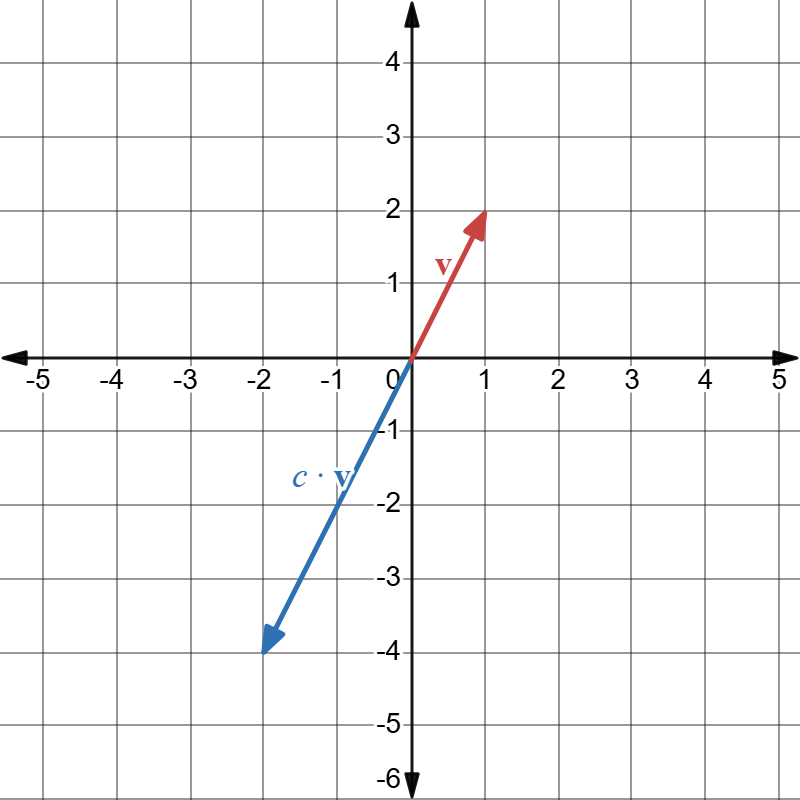
\includegraphics[width=0.5\linewidth]{chapters/chapter 2/y=2x 2.png}
\end{figure}

Պարզվում է՝ միայն $\R^2$-ը չէ, որ օժտված է այդ լավ հատկություններով։ Վերցնենք, օրինակ, $y=2x$ ուղիղը և դրա վրա ընտրենք ցանկացած $\vv$ վեկտոր։ Ինչպիսի $c\in \R$ թվով էլ այն բազմապատկենք, արդյունքում ստացված վեկտորը նորից ընկած է լինելու $y=2x$ ուղղի վրա։ Նույն կերպ, ինչ երկու $\vv_1$, $\vv_2$ վեկտորներ էլ վերցնենք այս ուղղի վրա և գումարենք իրար, ստացվածը կրկին $y=2x$-ի վրա է լինելու։ 

Այլ կերպ ասած՝ ինչպես $\R^2$-ը, այնպես էլ $y=2x$ ուղիղը (գիծը) \textbf{փակ է գումարման և թվով բազմապատկման նկատմամբ։} 

\question{Իսկ ի՞նչ կարող եք ասել $y=2x+1$ ուղղի մասին։}

Նմանատիպ օգտակար բազմությունները, որոնց տարրերը կարելի է ազատորեն
\begin{itemize}
    \item գումարել-հանել
    \item գումարելիների տեղերը փոխել
    \item գումարման ու թվով բազմապատկման հերթականությունը փոխել
    \item փակագծերը բացել
\end{itemize}
և այլն՝ առանց այդ բազմությունից դուրս\marginnote{
$\R^2$-ը գծային տարածություն է, իսկ $y=2x$ ուղիղը նրա ենթատարածություն է} հայտնվելու, կանվանենք \textit{գծային տարածություններ։} 

\begin{definition}
$V$ բազմությունը կոչվում է \textbf{գծային} (կամ վեկտո\-րա\-կան) \textbf{տարածություն,} եթե այն
\begin{enumerate}
\item փակ է գումարման և թվով բազմապատկման\marginnote{ցանկացած իրական թվով} նկատմամբ
\end{enumerate}
և նրա տարրերը բավարարում են հետևյալ հատկություններին․
\begin{enumerate}[resume]
  \item \( (\mathbf{u} + \mathbf{v}) + \mathbf{w} = \mathbf{u} + (\mathbf{v} + \mathbf{w}) \)
  \item \( \mathbf{u} + \mathbf{v} = \mathbf{v} + \mathbf{u} \)
  \item կա մի այնպիսի \( \mathbf{0} \) տարր, որ \( \mathbf{v} + \mathbf{0} = \mathbf{v} \) ցանկացած \( \mathbf{v} \in V \) համար
  \item ցանկացած \( \mathbf{v} \in V \) տարրի համար կա այնպիսի \( \overline{\vv} \) տարր,\marginnote{այսինքն՝ ամեն $\vv$-ի հակադիր ևս $V$-ից է} որ \( \mathbf{v} + \overline{\vv} = \mathbf{0} \)
  \item \( (cd) \cdot \mathbf{v} = c \cdot (d \cdot \mathbf{v}) \)
  \item \( 1 \cdot \mathbf{v} = \mathbf{v} \)
  \item \( c \cdot (\mathbf{u} + \mathbf{v}) = c \cdot \mathbf{u} + c \cdot \mathbf{v} \)
  \item \( (c + d) \cdot \mathbf{v} = c \cdot \mathbf{v} + d \cdot \mathbf{v} \)
\end{enumerate}
\end{definition}

Հատկությունները անգիր անելու կարիք չկա․ դրանք այն բնական հատկություններն են, առանց որոնց կդժվարանայինք աշխատել վեկտորների հետ։


\section{Ենթատարածություններ}


Այսպիսով, $\R^2$-ը ($\R^1$-ը, $\R^3$-ը, ...) գծային տարածություն է։ Բայց նրանում ընկած $y=2x$ ուղիղը նույնպես բավարարում է 1-9 պայման\-նե\-րին, հետևաբար այն նույնպես գծային տարածություն է։ 

\begin{definition}
$V$ գծային տարածության $U$ ենթաբազմությունը կոչվում է $V$-ի \textbf{ենթատարածություն,} եթե այն ինքը գծային տարածություն է։
\end{definition}

\begin{example} 
Գծային տարածություններ են օրինակ՝
\begin{itemize}
\item բոլոր $\R^n$-երը,

\item իրական թվերի $\R$ բազմությունը,

\item $\R^2$ հարթության $(0, 0)$ սկզբնակետով անցնող ցանկացած ուղիղ (հետևաբար դրանք $\R^2$-ի ենթատարածություններ են),

\item $\R^3$ տարածության $(0, 0, 0)$ սկզբնակետով անցնող ցանկացած ուղիղ և ցանկացած հարթություն (հետևաբար դրանք $\R^3$-ի ենթա\-տարածու\-թյուններ են),


\item միայն $\mathbf{0}$-ից բաղկացած $\{\mathbf{0}\}$ բազմությունը,
\end{itemize}
բայց միևնույն ժամանակ՝
\begin{itemize}
\item բնական թվերի բազմությունը,

\item դրական թվերի բազմությունը,

\item $\R^2$-ի՝ $y$-ների առանցքից վերև ընկած վեկտորների բազմությունը
\end{itemize}
գծային տարածություններ չեն։
\end{example}

Իրականում, եթե ունենք ինչ-որ $V$ գծային տարածություն և դրա մի որևէ $U$ ենթաբազմություն,\marginnote{որպես օրինակ՝ պատկերացրեք $V=\R^2$, իսկ $U$-ն $y=2x$ ուղիղն է $\R^2$-ում} ապա դժվար չէ պարզել՝ $U$-ն իրենով գծային (ենթա)տարածություն է, թե ոչ։ Պարզվում է, որ եթե $U$-ն փակ է գումարման և թվով բազմապատկման նկատմամբ, ապա դա \textit{բավարար} է, որ այն լինի $V$-ի ենթատարածություն։ 

\begin{theorem}
Եթե $V$-ն գծային տարածություն է, իսկ $U$-ն նրա որևէ ենթաբազմություն, ապա $U$-ն կլինի $V$-ի ենթատարածություն այն և միայն այն դեպքում, եթե  
\begin{enumerate}
\item $\vx+\vy \in U$ ցանկացած $\vx,\ \vy\in U$ համար,
\item $c\vx \in U$ ցանկացած $\vx\in U$ և $c\in\R$ համար։
\end{enumerate}
\end{theorem}

Այսինքն՝ եթե $U$-ն փակ է գումարման ու թվով բազմապատկման նկատմամբ, ապա մնացած 2-9 օգտակար հատկությունները այն արդեն ժառանգում է $V$-ից (հետևաբար դառնում գծային տարածություն)։

\warning{Թեորեմը աշխատում է, միայն եթե $V$-ն գծային տարածություն է։}



\section{Մատրիցներ}

Այժմ պատրաստվում ենք $\R^n$ տարածությունը պտտել, շրջել, ռեզինի նման ձգել ու սեղմել, բայց դրա համար նախ հարկավոր է ներմուծել մի գործիք։

Ի՞նչ կլինի, եթե իրար կողք շարենք մի քանի սյուն վեկտորներ (կամ իրար տակ՝ մի քանի տող վեկտորներ)․ կստացվի այդ վեկտորներից կազմված աղյուսակ։ $m$ տող և $n$ սյուն ունեցող թվերի աղյուսակը կանվանենք $m \times n$ չափանի \textbf{մատրից․}
\[
A =
\begin{bmatrix}
    a_{11} & a_{12} & \ldots & a_{1n} \\
    a_{21} & a_{22} & \ldots & a_{2n} \\
    \vdots & \vdots & \ddots & \vdots \\
    a_{m1} & a_{m2} & \ldots & a_{mn}
\end{bmatrix},
\qquad a_{ij} \in \mathbb{R}։
\]
\begin{marginfigure}

\includegraphics{chapters//chapter 2/keanu.png}
\end{marginfigure}
Մատրիցները որպես կանոն կնշանակենք լատինական մեծատառերով, իսկ դրանց տարրերը՝ փոքրատառ + ինդեքսում սյան և տողի համարով (օրինակ՝ $4$-րդ տողի $6$-րդ թվի դեպքում $a_{46}$)։ 

Ինչպես վեկտորների դեպքում, բոլոր $m \times n$ չափանի մատրիցների բազմությունը կնշանակենք $\R^{m\times n}$-ով։

\warning{Առաջինը միշտ նշում ենք տողը, հետո՝ սյունը։}

\begin{example}
\[
  A = \begin{bmatrix}
    1 & 2 & 3 \\
    4 & 5 & 6 \\
  \end{bmatrix} \in \R^{2\times 3}
  \qquad
  B = \begin{bmatrix}
    -2 & 0 \\
    1 & 3 \\
  \end{bmatrix} \in \R^{2\times 2}
\]
\end{example}

\question{Որո՞նք են $m \times 1$ չափանի մատրիցները։}


 
\section{Գործողություններ մատրիցների հետ}

Մատրիցները կգումարենք, հանենք, թվով բազմապատկենք ճիշտ այնպես, ինչպես վեկտորները, այսինքն՝ տարր առ տարր։

\begin{description}
\item[Գումարում․]  Նույն չափանի երկու մատրիցներ գումարելիս համապա\-տաս\-խան տեղում գրված տարրերը գումարվում են իրար՝
\[
  A = \begin{bmatrix}
    a_{11} & a_{12} & \ldots & a_{1n} \\
    a_{21} & a_{22} & \ldots & a_{2n} \\
    \vdots & \vdots & \ddots & \vdots \\
    a_{m1} & a_{m2} & \ldots & a_{mn} \\
  \end{bmatrix}
  \qquad
  B = \begin{bmatrix}
    b_{11} & b_{12} & \ldots & b_{1n} \\
    b_{21} & b_{22} & \ldots & b_{2n} \\
    \vdots & \vdots & \ddots & \vdots \\
    b_{m1} & b_{m2} & \ldots & b_{mn} \\
  \end{bmatrix}
\]

\[
  A + B = \begin{bmatrix}
    a_{11} + b_{11} & a_{12} + b_{12} & \ldots & a_{1n} + b_{1n} \\
    a_{21} + b_{21} & a_{22} + b_{22} & \ldots & a_{2n} + b_{2n} \\
    \ldots & \ldots & \ldots & \ldots \\
    a_{m1} + b_{m1} & a_{m2} + b_{m2} & \ldots & a_{mn} + b_{mn} \\
  \end{bmatrix}
\]

\item[Թվով բազմապատկում․] Մատրիցը $c \in \R$ թվով (սկալյարով) բազմա\-պատ\-կելիս դրա բոլոր տարրերը բազմապատկում ենք $c$-ով՝
\[
  c \cdot A = c \cdot \begin{bmatrix}
    a_{11} & a_{12} & \ldots & a_{1n} \\
    a_{21} & a_{22} & \ldots & a_{2n} \\
    \vdots & \vdots & \ddots & \vdots \\
    a_{m1} & a_{m2} & \ldots & a_{mn} \\
  \end{bmatrix}= \begin{bmatrix}
    c \cdot a_{11} & c \cdot a_{12} & \ldots & c \cdot a_{1n} \\
    c \cdot a_{21} & c \cdot a_{22} & \ldots & c \cdot a_{2n} \\
    \vdots & \vdots & \ddots & \vdots \\
    c \cdot a_{m1} & c \cdot a_{m2} & \ldots & c \cdot a_{mn} \\
  \end{bmatrix}
\]


\item[Հակադիր․] Մատրիցի հակադիրը նույն մատրիցն է՝ բազմապատկած $-1$-ով, այսինքն՝ բոլոր թվերը փոխարինած իրենց հակադիրներով․
\[
  -A = \begin{bmatrix}
    -a_{11} & -a_{12} & \ldots & -a_{1n} \\
    -a_{21} & -a_{22} & \ldots & -a_{2n} \\
    \ldots & \ldots & \ldots & \ldots \\
    -a_{m1} & -a_{m2} & \ldots & -a_{mn} \\
  \end{bmatrix}
\]

\item[Հանում․]  Նույն չափանի մի մատրիցից մյուսը հանելիս առաջինի տարրերից հանում ենք երկրորդի համապատասխան տեղում գրված տարրերը՝
\[
  A - B = \begin{bmatrix}
    a_{11} - b_{11} & a_{12} - b_{12} & \ldots & a_{1n} - b_{1n} \\
    a_{21} - b_{21} & a_{22} - b_{22} & \ldots & a_{2n} - b_{2n} \\
     \ldots & \ldots & \ldots & \ldots \\
    a_{m1} - b_{m1} & a_{m2} - b_{m2} & \ldots & a_{mn} - b_{mn} \\
  \end{bmatrix}
\]
\end{description}

Ինչպես տեսնում ենք, գործողությունների տրամաբանությունը նույնն է, ինչ վեկտորների դեպքում։ Այստեղ նույնպես

\warning{Տարբեր չափ ունեցող մատրիցներ գումարել և հանել չենք կարող։}

Ինչպես կարելի է կռահել, ամբողջությամբ զրոներից բաղկացած մատրիցը կոչվում է \textit{զրոյական մատրից} և նշանակվում $O$ կամ $O_{m \times n}$։\marginnote{$m$-ն ու $n$-ը մատրիցի չափերն են}

\begin{example}
\[
  O_{2 \times 3} = \begin{bmatrix}
    0 & 0 & 0 \\
    0 & 0 & 0 \\
  \end{bmatrix}
  \qquad
  O_{3 \times 2} = \begin{bmatrix}
    0 & 0 \\
    0 & 0 \\
    0 & 0 \\
  \end{bmatrix}
\]
\end{example}

\question{Ի՞նչ կստացվի, եթե որևէ մատրիցի ձախից գումարենք $O$: \linebreak Իսկ աջի՞ց։}

Մինչ այս պահը բոլոր գործողությունները սահմանել ենք շատ բնական ձևով, ինչպես վեկտորների դեպքում։ Ուստի զարմանալի չէ, որ ցանկացած ֆիքսած $m$, $n$-ի համար 
\begin{theorem}
$\R^{m \times n}$ բազմությունը գծային տարածություն է։
\end{theorem}
Այսինքն՝ ֆիքսված չափի մատրիցների բազմությունը և նրա վրա մեր սահմանած գումարումն ու թվով բազմապատկումը բավարարում են 1-9 օգտակար հատկություններին։ Այլ կերպ ասած՝ մատրիցների հետ գործողություններ անելիս կարելի է հանգիստ փակագծերը բացել, գումարելիների տեղերը փոխել, և այլն։

\question{Կարո՞ղ եք ապացուցել թեորեմը։}

Վերջապես սահմանենք նաև մատրիցի շրջումը։

\begin{definition}
$A$ մատրիցի \textbf{տրանսպոնացված} (կամ \textbf{շրջած}) ենք անվանում նույն մատրիցը՝ տողերի փոխարեն գրած $A$-ի սյուները/սյուների փոխարեն գրած $A$-ի տողերը․ 
\[
A = \begin{bmatrix}
    a_{11} & a_{12} & \ldots & a_{1n} \\
    a_{21} & a_{22} & \ldots & a_{2n} \\
     \ldots & \ldots & \ldots & \ldots  \\
    a_{m1} & a_{m2} & \ldots & a_{mn} \\
  \end{bmatrix}\qquad A^T = \begin{bmatrix}
    a_{11} & a_{21} & \ldots & a_{n1} \\
    a_{12} & a_{22} & \ldots & a_{n2} \\
     \ldots & \ldots & \ldots & \ldots  \\
    a_{1m} & a_{2m} & \ldots & a_{nm} \\
  \end{bmatrix}
\]
\end{definition}

\begin{example}
\[
  A = \begin{bmatrix}
    7&4&2\\0&1&-3
  \end{bmatrix}\qquad
  A^T = \begin{bmatrix}
    7 & 0 \\
    4 & 1 \\
    2 & -3
  \end{bmatrix}
\]
\end{example}

Նկատենք, որ եթե $A \in \R^{m \times n}$, ապա $A^T \in \R^{n \times m}$:


\section{Մատրիցի և վեկտորի բազմապատկումը}

Այժմ ունենք երկու տեսակի օբյեկտ՝ վեկտորներ և մատրիցներ, որոնք մինչ այս ապրել են իրենց առանձին աշխարհներում։ Ժամանակն է սահմանել մի բան, որը իրար կկապի մատրիցներն ու վեկտորը։ 

\begin{definition}\label{mvm}
Ենթադրենք $A$-ն \(m \times n\) մատրից է, իսկ \(\mathbf{v}\)-ն՝ $n$-չափանի վեկտոր։ $A$ մատրիցը և $\vv$ վեկտորը բազմապատկելու համար $A$-ի յուրաքանչյուր տողում գրված թվերը հերթով բազմապատկում ենք $\vv$-ի համապատասխան տարրերի հետ և ստացված արտադրյալները գումարում։ 
\[
  A = \begin{bmatrix}
    a_{11} & a_{12} & \ldots & a_{1n} \\
    a_{21} & a_{22} & \ldots & a_{2n} \\
    \vdots & \vdots & \ddots & \vdots \\
    a_{m1} & a_{m2} & \ldots & a_{mn} \\
  \end{bmatrix}
  \qquad
  \mathbf{v} = \begin{bmatrix}
    v_1 \\
    v_2 \\
    \vdots \\
    v_n \\
  \end{bmatrix}
\]\begin{marginfigure}    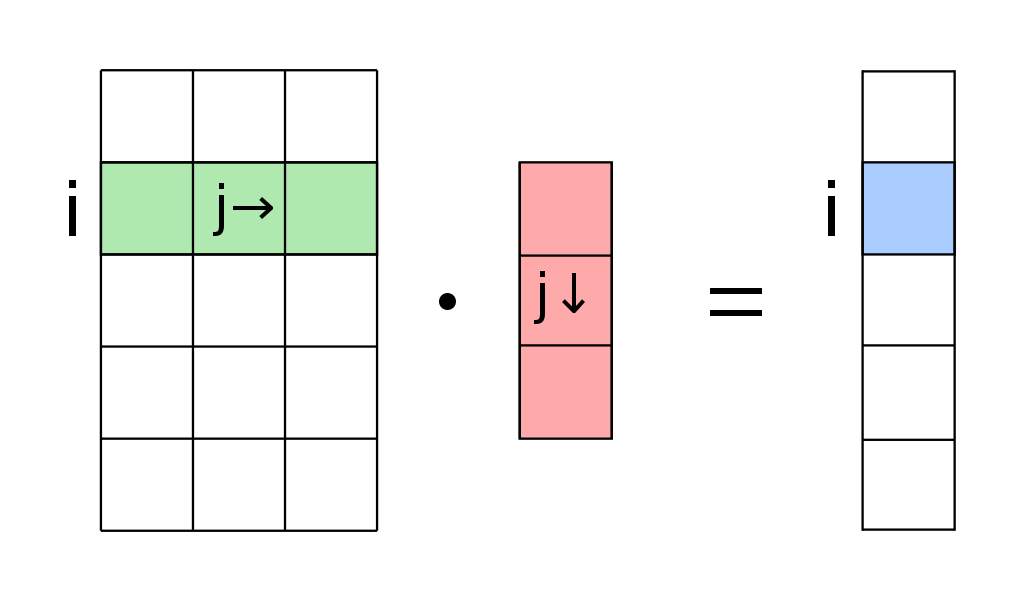
\includegraphics[width=\textwidth, height=\textheight, keepaspectratio]{chapters/chapter 2/mvm.png}
\end{marginfigure}\[
  A\mathbf{v} = \begin{bmatrix}
    a_{11}v_1 + a_{12}v_2 + \ldots + a_{1n}v_n \\
    a_{21}v_1 + a_{22}v_2 + \ldots + a_{2n}v_n \\
    \vdots \\
    a_{m1}v_1 + a_{m2}v_2 + \ldots + a_{mn}v_n \\
  \end{bmatrix}
\]
Արդյունքում ստացված $m$-չափանի վեկտորը կոչվում է \textbf{$A$ մատրիցի և $\vv$ վեկտորի արտադրյալ։} 
\end{definition}

Այլ կերպ ասած՝ եթե $A$-ի տողերը նշանակենք $\mathbf{A}_1, \mathbf{A}_2, \ldots, \mathbf{A}_m$՝\marginnote{\bigskip \bigskip \bigskip \bigskip $\mathbf{A}_i$-երը կլինեն $n$-չափանի վեկտորներ}
\[
A = \begin{bmatrix}
\dots& \mathbf{A}_1 & \ldots \\
\dots& \mathbf{A}_2 & \ldots \\
 & \vdots &  \\
\dots& \mathbf{A}_m & \ldots \\
\end{bmatrix}
\]
ապա 
\begin{itemize}
\item $A\vv$-ի առաջին բաղադրիչը կլինի $\mathbf{A}_1 \cdot \vv$ սկալյար արտադրյալը,
\item $A\vv$-ի երկրորդ բաղադրիչը կլինի $\mathbf{A}_2 \cdot \vv$ սկալյար արտադրյալը,
\end{itemize}
և այդպես շարունակ՝
\[
A\mathbf{v} = \begin{bmatrix}
a_{11}v_1 + a_{12}v_2 + \ldots + a_{1n}v_n \\
a_{21}v_1 + a_{22}v_2 + \ldots + a_{2n}v_n \\
\vdots \\
a_{m1}v_1 + a_{m2}v_2 + \ldots + a_{mn}v_n \\
\end{bmatrix}= \begin{bmatrix}
\mathbf{A}_1 \cdot \mathbf{v} \\
\mathbf{A}_2 \cdot \mathbf{v} \\
\vdots \\
\mathbf{A}_m \cdot \mathbf{v} \\
\end{bmatrix} 
\]

\begin{example}
\[
  A = \begin{bmatrix}
    1 & 2 & 3 \\
    4 & 5 & 6 \\
  \end{bmatrix}
  \qquad
  \mathbf{v} = \begin{bmatrix}
    2 \\
    -1 \\
    3 \\
  \end{bmatrix}
\]
\[
  A\mathbf{v} = \begin{bmatrix}
    1 \cdot 2 + 2 \cdot (-1) + 3 \cdot 3 \\
    4 \cdot 2 + 5 \cdot (-1) + 6 \cdot 3 \\
  \end{bmatrix}
  = \begin{bmatrix}
    9 \\
    21 \\
  \end{bmatrix}
\]
\end{example}

Ինչ-որ իմաստով՝ մատրիցի ու վեկտորի բազմապատկումը մեր իմացած սկալյար արտադրյալի ընդհանրացումն է։ Ի սկզբանե գիտեինք, թե ինչպես բազմապատկել վեկտորը վեկտորով։ Իսկ մատրիցը ոչ այլ ինչ է, քան իրար տակ գրված մի քանի վեկտոր։ Ինչպե՞ս պիտի բազմապատկեինք այդ «մի քանի վեկտորը» մեկ այլ $\vv$ վեկտորի հետ․ բնական կլիներ հերթով դրանցից յուրաքանչյուրը բազմապատկել $\vv$-ով, ապա ստացվածները գրել իրար տակ (ինչը և արեցինք)։

\begin{example}
\[
  A = \begin{bmatrix}
    -2 & 1 \\
    0 & 3 \\
    1 & -1 \\
  \end{bmatrix}
  \qquad
  \mathbf{v} = \begin{bmatrix}
    4 \\
    2 \\
  \end{bmatrix}
\]
\[
  A\mathbf{v} = \begin{bmatrix}
    (-2) \cdot 4 + 1 \cdot 2 \\
    0 \cdot 4 + 3 \cdot 2 \\
    1 \cdot 4 + (-1) \cdot 2 \\
  \end{bmatrix}
  = \begin{bmatrix}
    -6 \\
    6 \\
    2 \\
  \end{bmatrix}
\]
\end{example}


Այնուամենայնիվ, ինչո՞ւ պետք է ուզենք վեկտորը բազմապատկել մատրիցով։
Մտովի պատկերեք տարածության մեջ մի քանի վեկտոր՝ որպես սլաքներ։\marginnote{\href{https://visualize-it.github.io/linear_transformations/simulation.html}{այստեղ} սեղմելով {\rm transform}՝ կտես\-նեք, թե ինչ է տեղի ունենում վեկ\-տորները բեր\-ված մատրիցով բազմապատկելիս}
Ինչպես կտեսնենք հաջորդ թեմայում, վեկտորները մատրիցով բազմապատկելը երկրաչափորեն նույնն է, ինչ այդ վեկտոր\-ները ինչ-որ մի անկյան տակ պտտելը, և դրանց ինչ-որ ուղղությամբ սեղմելը կամ ձգելը։ Այլ կերպ ասած՝ երբ վեկտորները բազմապատկում ենք մատրիցով, դրանք \textit{ձևափոխվում} են։ 

Ընդ որում՝ այդ ձևափոխությունը տեղի ունենալու ժամանակ պահպան\-վում են հետևյալ կանոնները՝
\begin{enumerate}
    \item $A(\vv+\vu)=A\vv + A\vu$
    \item $A(c \cdot \vv) = c \cdot A\vv$
\end{enumerate}
այսինքն՝ 
\begin{enumerate}
    \item ձևափոխել, հետո գումարել $=$ գումարել, հետո ձևափոխել
    \item ձգել, հետո ձևափոխել $=$ ձևափոխել, հետո ձգել
\end{enumerate}

Այս հատկությունների շնորհիվ մատրիցով բազմապատկման գործո\-ղու\-թյունը կանվանենք նաև \textit{գծային ձևափոխություն,} և կասենք՝ $A$ մատրիցը/գծային ձևափոխությունը \textbf{կիրառել} $\vv$ վեկտորի վրա։ Այս մասին ավելի մանրամասն կխոսենք հաջորդ թեմայում։

\question{Ի՞նչ մատրից կիրառենք $[4 \quad 5]$ վեկտորի վրա, որպեսզի այն երկու անգամ ձգվի։}



\section{Մատրիցների բազմապատկումը}

Եվ իհարկե, սահմանենք երկու մատրիցների արտադրյալը՝ մոտա\-վո\-րա\-պես նույն տրամաբանությամբ։

\begin{definition}\label{mmm}
Ենթադրենք $A$-ն \(m \times n\) մատրից է, իսկ $B$-ն՝ $n \times k$ մատրից։\marginnote{$A$-ի սյուների թիվ $=$ $B$-ի տողերի թիվ} $A$ և $B$ \textbf{մատրիցների արտադրյալը} կլինի $m \times k$ չափանի մատրից, որի $i$-րդ տողի $j$-րդ տարրը հավասար է $A$-ի $i$-րդ տողի և $B$-ի $j$-րդ սյան սկալյար արտադրյալին։
\[
A = \begin{bmatrix}
a_{11} & a_{12} & \ldots & a_{1n} \\
a_{21} & a_{22} & \ldots & a_{2n} \\
\dots & \dots & \dots & \dots \\        a_{m1} & a_{m2} & \ldots & a_{mn} \\
\end{bmatrix}
\qquad
B = \begin{bmatrix}
b_{11} & b_{12} & \ldots & b_{1k} \\
b_{21} & b_{22} & \ldots & b_{2k} \\
\dots & \dots & \dots & \dots \\        b_{n1} & b_{n2} & \ldots & b_{nk} \\
\end{bmatrix}
\]\begin{marginfigure}    
\includegraphics[width=\textwidth, height=\textheight, keepaspectratio]{chapters/chapter 2/mmm.png}
\end{marginfigure}\[
AB = \begin{bmatrix}
c_{11} & c_{12} & \ldots & c_{1k} \\
c_{21} & c_{22} & \ldots & c_{2k} \\
\dots & \dots & \dots & \dots \\
c_{m1} & c_{m2} & \ldots & c_{mk} \\
\end{bmatrix}
\]
որտեղ $\displaystyle c_{ij} = a_{i1}b_{1j} + a_{i2}b_{2j} + \ldots + a_{in}b_{nj}= \sum_{p=1}^{n} a_{ip}b_{pj}$:
\end{definition}

Այսինքն՝ ձախ մատրիցի ամեն մի տողը բազմապատկում ենք (սկալյա\-րա\-պես) աջ մատրիցի ամեն մի սյան հետ։

\begin{example}
\[
  C = \begin{bmatrix}
    -1 & 0 \\
    2 & -3 \\
    4 & 1 \\
  \end{bmatrix}\in \R^{3 \times 2}
  \qquad
  D = \begin{bmatrix}
    5 & -2 & 1 \\
    3 & 0 & 7 \\
  \end{bmatrix}\in \R^{2 \times 3}
\]
\begin{align*}
  CD &= \begin{bmatrix}
    -1 \cdot 5 + 0 \cdot 3 & -1 \cdot (-2) + 0 \cdot 0 & -1 \cdot 1 + 0 \cdot 7 \\
    2 \cdot 5 + (-3) \cdot 3 & 2 \cdot (-2) + (-3) \cdot 0 & 2 \cdot 1 + (-3) \cdot 7 \\
    4 \cdot 5 + 1 \cdot 3 & 4 \cdot (-2) + 1 \cdot 0 & 4 \cdot 1 + 1 \cdot 7 \\
  \end{bmatrix}
 \\&= \begin{bmatrix}
    -5 & 2 & -1 \\
    1 & -4 & -19 \\
    23 & -8 & 11 \\
  \end{bmatrix}\in\R^{3 \times 3}
\end{align*}
\end{example}

\question{Ի՞նչ կստացվեր, եթե վերևի օրինակում բազմապատկեինք այսպես՝ $DC$։}


\warning{Երկու մատրից հնարավոր է բազմապատկել միայն եթե առաջին մատրիցի սյուների թիվը (այսինքն՝ դրա տողերի երկարությունը) համընկնում են երկրորդի տողերի թվի (սյուների երկարության) հետ։}

Հետևաբար ոչ բոլոր մատրիցներն է հնարավոր իրարով բազմապատկել։

\question{Հնարավո՞ր է, որ երկու $A$, $B$ մատրից կարելի լինի բազ\-մա\-պատկել այսպես՝ $AB$, բայց ոչ այսպես՝ $BA$:}

Եթե չիմանայինք վեկտորների սկալյար արտադրյալի մասին, շատ տարօրինակ կլիներ մատրիցների արտադրյալը այս ձևով սահմանելը (իրոք, կարող էինք պարզապես բազմապատկումը սահմանել ասենք՝ տարր առ տարր)։ 

Իսկ այսպես սահմանելու դեպքում, եթե փորձեք օրինակ՝ ինչ-որ $A$ մատրից բազմապատկել $\vv$ վեկտորով, անկախ նրանից՝ $\vv$-ն կհամարեք վեկտոր \marginnote{նկատենք, որ $\va \cdot \vb = \va^T \vb$} և կօգտվեք \hyperref[mvm]{\color{OliveGreen} սահմանում \ref*{mvm}}-ից, թե կհամարեք այն $1$ սյունից բաղկացած մատրից ու կօգտվեք \hyperref[mmm]{\color{OliveGreen} սահմանում \ref*{mmm}}-ից, երկու դեպքում էլ կստանաք նույնը։

Նկատենք նաև, որ ինչպես բոլոր նախորդ գործողություններում, մատրիցների բազմապատկումը նույնպես օժտված է հետևյալ լավ հատկություններով՝
\begin{itemize}
\item $A(B + C) = AB + AC$ և  $(A + B)C = AC + BC$\marginnote{փակագծերը կարող ենք բացել}

\item $A(BC) = (AB)C$ \marginnote{կարևոր չէ՝ սկզբից $BC$-ն, թե $AB$-ն}

\item $A(cB) = c(AB)=(cA)B$\marginnote{ցանկացած $c\in\R$ թվի համար}
\end{itemize}



\bigskip 

\begin{theory}
.
\begin{itemize}
\item կարդալ [{\rm Johnston}], 121-124 (գծային տարածություններ), 35-38 (գծային ձևափոխություններ) էջերը
\item կարդալ [{\rm Poole}], 219-221 էջերը (մատրիցների արտադրյալ)
\item դիտել  {\rm 3b1b}-ի \href{https://www.3blue1brown.com/lessons/linear-transformations}{3-րդ տեսադասը} գծային հանրահաշվից \end{itemize}
\end{theory}

\newpage

\section{Խնդիրներ}

\begin{problem}\marginnote[*+0.5]{\href{https://youtu.be/N8GR7eCepl8}{նման խնդրի լուծում}}
Արդյո՞ք տրված բազմությունը գծային տարածություն է․

\begin{enumerate}[label={\alph*}․]
\item $A = \bigg\{ \begin{bmatrix} a \\ 0 \end{bmatrix} \mid \text{ բոլոր }a\in\R \text{ թվերի համար} \bigg\}$

\item \marginnote{\medskip $\R^2$ հարթության ո՞ր ուղիղն է սա}$B = \bigg\{ \begin{bmatrix} a \\ -a \end{bmatrix} \mid  \text{բոլոր }a\in\R \text{ թվերի համար} \bigg\}$

\item $C =  \bigg\{ \begin{bmatrix} a \\ 1 \end{bmatrix} \mid \text{ բոլոր }a\in\R \text{ թվերի համար}\bigg\}$

\item $D = \mathbb{Z}$ ամբողջ թվերի բազմությունը

\item $ax+b$ տեսքի բոլոր բազմանդամների բազմությունը

\item $ax+b$ տեսքի այն բազմանդամների բազմությունը, որոնցում $a \ne 0$
\end{enumerate}
\end{problem}


\hint{Եթե ցույց տանք, որ 1-9 պայմաններից գոնե մեկը խախտվում է, ապա բազմությունը գծային տարածություն չէ։ Եթե բոլոր 1-9 պայմանները միշտ տեղի ունեն, ապա բազմությունը գծային տարածություն է։}


\begin{problem}
Ի՞նչ կստանանք
\[
A = \begin{bmatrix}
    3 & -3 \\
    3 & 3
\end{bmatrix}
\] 
մատրիցը կիրառելով հետևյալ վեկտորների վրա․
\begin{enumerate}[label={\alph*}․]
\item $\va=\begin{bmatrix}
    1 \\ 0
\end{bmatrix}$

\item $\vb=\begin{bmatrix}
    0 \\ 1
\end{bmatrix}$

\item $\vc=\begin{bmatrix}
    1 \\ 1
\end{bmatrix}$
\end{enumerate}

Կոորդինատային հարթության վրա պատկերեք վեկտորներից յուրաքան\-չ\-յու\-րը մինչև $A$-ով բազմապատկելը և դրանից հետո։ Ի՞նչ եք տեսնում, ի՞նչ է անում մատրիցը վեկտորների հետ։ Կարո՞ղ եք գուշակել, թե ինչպես կձևափոխվի $\begin{bmatrix}
    2 & -2
\end{bmatrix}$ վեկտորը։
\end{problem}

\begin{problem}
Հաշվեք մատրիցների արտադրյալը․
\begin{enumerate}[label={\alph*}․]
\item $AB$, որտեղ $A=\begin{bmatrix}
6&5\\-2&7  \end{bmatrix}$, $B=\begin{bmatrix}
-5&3\\1&4   \end{bmatrix}$

\item $(A-B)(A+B)$, որտեղ $A=\begin{bmatrix}
2&2&4\\-3&-2&4\\-2&0&2   \end{bmatrix}$, $B=\begin{bmatrix}
2&1&3\\-1&2&2\\1&4&-1   \end{bmatrix}$

\item $A^2 - B^2$, նույն $A$ ու $B$-ով, ինչ \textit{բ․}-ում
\end{enumerate}

Նո՞ւյնն են արդյոք \textit{բ․}-ում ու \textit{գ․}-ում ստացված մատրիցները։
\end{problem}

\begin{problem}
Դիտարկենք հետևյալ մատրիցը (կոչվում է \textit{շեղման} կամ \textit{սահքի մատրից})՝\marginnote{անգլերեն՝ {\it shear matrix}}
\[
S = \begin{bmatrix}
    1 & 1 \\ 0 & 1
\end{bmatrix}
\]
\begin{enumerate}[label={\alph*}․]
\item ի՞նչ կստանանք, եթե $S$-ը կիրառենք $\begin{bmatrix}
    0 & 1
\end{bmatrix}$ վեկտորի վրա

\item ի՞նչ կստանանք, եթե $S$-ը կիրառենք ստացված վեկտորի վրա

\item ի՞նչ կստանանք, եթե մի անգամ էլ կիրառենք $S$-ը

\item ի՞նչ եք կարծում, ի՞նչ կստանանք, եթե $S$-ը կիրառենք $100$ անգամ այդ վեկտորի վրա

\item կարո՞ղ եք հաշվել $S^{100}$-ը
\end{enumerate}
\end{problem}


\begin{problem}\marginnote{\bigskip \href{https://youtu.be/fM2H49xwXS8}{լուծում}}
Ենթադրենք $A$-ն այնպիսի մատրից է, որ
\[
A\begin{bmatrix}
    1 \\ 2
\end{bmatrix}
=
\begin{bmatrix}
    -3 \\ 5
\end{bmatrix},
\qquad 
A\begin{bmatrix}
    3 \\ 5
\end{bmatrix}
=
\begin{bmatrix}
    7 \\ 1
\end{bmatrix}
\]
Քանի՞սը քանիսի վրա է $A$ մատրիցը։ Գտեք $A$-ն։
\end{problem}









% \begin{problem}
% Տրված են հետևյալ վեկտորները՝
% \[
% \va= \begin{bmatrix} 3 \\ -1 \\ 2 \end{bmatrix}, \qquad \vb=\begin{bmatrix} 2 \\ 4 \\ -5 \end{bmatrix}, \qquad \vc = \begin{bmatrix}
%     5 \\ 6.5 \\ -7
% \end{bmatrix}
% \]

% Գտեք արտահայտության արժեքը․
% \begin{enumerate}[label={\alph*}․]
% \item $\va+\vb$
% \item $\va+\vb-\vc$
% \item $\va^T+\vb^T-\vc^T$
% \item $3\va^T+4\vb^T-2\vc^T$
% \item $6\va^T+8\vb^T-4\vc^T$
% \item $\va \cdot \vb$
% \item $(3\va - 6\vb) \cdot \vc$
% \item $\va \cdot (4\va^T - \vb^T)^T$
% \end{enumerate}
% \end{problem}

% \begin{problem}
% Թարգմանչական գրասենյակը թարգմանեց  $\va=\begin{bmatrix}
%     24 & 17 & 9 & 13
% \end{bmatrix}$ փաստաթուղթ համապատասխանաբար անգլերեն, ֆրանսերեն, գերմաներեն և ռուսերեն։ Յուրաքանչյուր լեզվի համար մեկ էջ թարգմանելը տևում է մոտավորապես $\vb=\begin{bmatrix}
%     5 & 10 & 11 & 7
% \end{bmatrix}$ րոպե։ 

% \smallskip

% Ընդհանուր որքա՞ն ժամանակ պահանջվեց փաստաթղթերը թարգմանելու համար։ Միջինում քանի՞ րոպե ծախսեց թարգմանիչներից յուրաքանչյուրը, եթե գրասենյակում կա $4$ թարգմանիչ։ Պատասխանը արտահայտեք $\va$-ով և $\vb$-ով։
% \end{problem}

% \begin{problem}
% Հաշվեք հետևյալ վեկտորների մանհեթընյան և էվկլիդյան նորմերը․

% \begin{enumerate}[label={\alph*}․]
% \item $\va= \begin{bmatrix} 2\\-9\\3 \end{bmatrix}$

% \item $\va-2\vb$, որտեղ $\va= \begin{bmatrix}3\\4\\1\\0\end{bmatrix},\  \vb = \begin{bmatrix}4\\5\\-2\\-1\end{bmatrix}$

% \item $-3\vc$, որտեղ $\vc= \begin{bmatrix}2\\-5\\6\end{bmatrix}$
% \end{enumerate}
% \end{problem}

% \begin{problem}
% Որքա՞ն անկյուն են կազմում
% \begin{enumerate}[label={\alph*}․]
% \item $\va= \begin{bmatrix} 2\\1\\1\end{bmatrix}$ և $\vb= \begin{bmatrix} 1\\-3\\3\end{bmatrix}$ վեկտորները

% \item նախորդ խնդրի $\va$ ու $\vc$ վեկտորները
% \end{enumerate}
% \end{problem}


% \begin{problem}
% Ամենաշատը քանի՞ վեկտոր կարող ենք տեղադրել $\R^2$ հարթության մեջ, որպեսզի ցանկացած երկուսի սկալյար արտադրյալը լինի դրական։ Իսկ որպեսզի լինի բացասակա՞ն։
% \end{problem}

\setchapterpreamble[u]{\margintoc}
\chapter{Երկրաչափական մեկնաբանություն}
\labch{geometry}

\emergencystretch 2em

\section{Գծային ձևափոխու\-թյուն\-ները երկրաչափորեն}

Նախորդ թեմայից հետո ծագում է հետևյալ հարցը․

\textit{— Ուրեմն մատրից $=$ թվերի աղյուսակ, այդքան բա՞ն}

Շտապենք հանգստացնել․ պատասխանն է՝ ոչ, բացարձակապես ոչ, մատրիցներն ընդամենը թվերի աղյուսակներ չեն, և Դուք ստիպված չեք լինելու ձանձրալի ու անհետաքրքիր թվեր բազմապատկելով զբաղվել։ 
Ինչպես ամեն վեկտոր ոչ այլ ինչ է, քան տարածության մեջ ինչ-որ մի սլաք, այդպես էլ մատրիցները՝ գծային ձևափոխությունները, գեղեցիկ երկրաչափական գաղափարներ են։ 

Պատկերացրեք՝ թղթի վրա նկարել ենք կոորդինատային առանցքները և մի քանի վեկտորներ։ Եթե ենթադրենք, որ թուղթը ռեզինից է, և ձգել-սեղմելուց չի պատռվում, այլ լոճվում է, ապա կարող ենք այն, օրինակ,
\begin{itemize}
    \item պտտել $40^\circ$-ով
    \item ձախ ու աջ կողմերից ձեռքով բռնել և ձգել
    \item վերևից ու ներքևից բռնել և ներս սեղմել
    \item վերևից ու ներքևից բռնել և ներս սեղմել, ապա $15^\circ$-ով պտտել
\end{itemize}
\begin{marginfigure}    \begin{center}
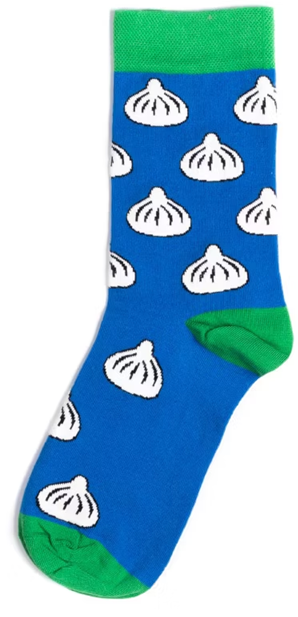
\includegraphics[width=0.55\textwidth, height=\textheight, keepaspectratio]{chapters/chapter 3/khinkali.png}
\end{center}
\caption*{ի՞նչ կլինի խինկալիների հետ, եթե գուլ\-պան ձախից ու աջից բռնենք և քաշենք}
\end{marginfigure}
Ամեն անգամ թղթի վրայի բոլոր վեկտորները իրենց նախորդ դիրքի համեմատ կպտտվեն, կձգվեն, կսեղմվեն, այսինքն՝ կձևափոխվեն ինչպես մնացած վեկտորները։  Ահա հենց այդպիսի ազդեցություն է լինում, երբ տարածության մեջ ինչ-որ վեկտորներ բազմապատկում ենք մատրիցով։

\begin{figure}[h]
    \centering
    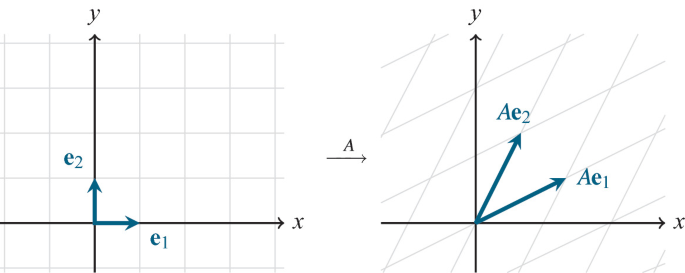
\includegraphics[width=0.75\linewidth]{chapters/chapter 3/viz ex.png}
\end{figure}

Իրոք, ի՞նչ է տեղի ունենում, երբ օրինակ՝ $2\times 2$ չափանի $A$ մատրիցը կիրառում ենք $\vv\in\R^2$ վեկտորի վրա․ ստանում ենք մեկ այլ՝ նոր $\vu=A\vv\in\R^2$ վեկտոր։ Այս նոր, ձևափոխված $\vu$ վեկտորը նույն հին ու բարի $\vv$-ն է՝ պարզապես ինչ-որ անկյան տակ \textbf{պտտած, ձգած} կամ \textbf{սեղմած} և, հնարավոր է, \textbf{շրջած} ({\rm flip} արած)։ Թե քանի աստիճանով պտտած և հորիզոնական/ուղղաձիգ ուղղությամբ քանի անգամ է այն ձգած՝ կախված է մատրիցի մեջ գրված թվերից, բայց բուն գաղափարն այն է, որ տրված $A$ մատրիցը \textit{ինչ գործողություններ որ անում է որևէ վեկտորի հետ, նույն \marginnote{գործողություն $=$ պտույտ, ձգում, սեղ- \linebreak մում, շրջում (որոշ հերթականությամբ)}գործողությունները անում է նաև բոլոր մյուս վեկտորների հետ,} այն այդ վեկտորների վրա կիրառելիս։

Այլ կերպ ասած՝ եթե վեկտորները տարածության մեջ սլաքներ են, ապա մատրիցները այդ սլաքների պտտումները, ձգումները, սեղմումներն ու շրջումներն են։

\begin{figure}[t]
    \label{mona}
    \centering
    % \subfloat[\centering label 1]{{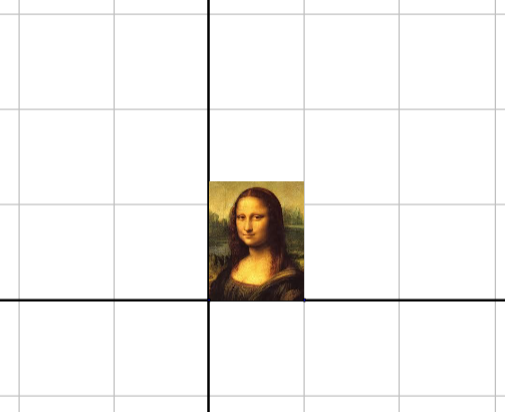
\includegraphics[width=0.4\linewidth]{chapters/chapter 3/mona_1.png} }}%
    \subfloat{{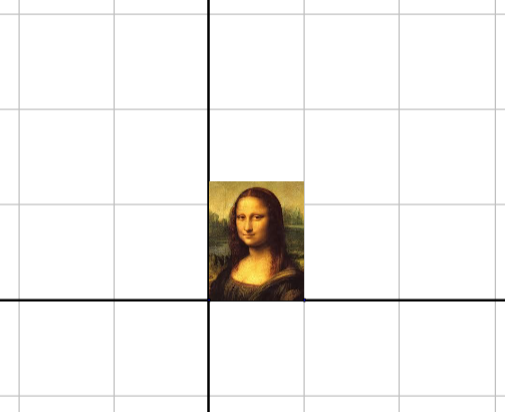
\includegraphics[width=0.4\linewidth]{chapters/chapter 3/mona_1.png} }}%
    \qquad
    \subfloat{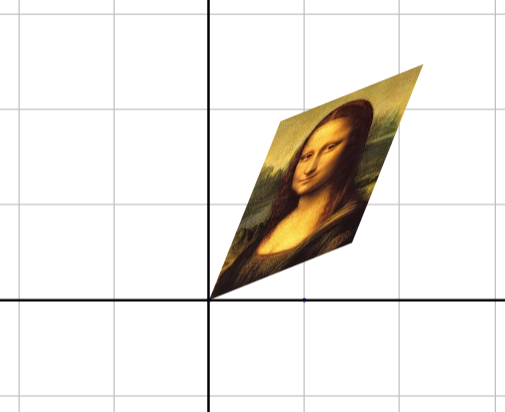
\includegraphics[width=0.4\linewidth]{chapters/chapter 3/mona_2.png}} %
    \caption*{Մոնա Լիզան՝ $$M = \begin{bmatrix}
        1.5 & 0.6 \\ 0.6 & 1.5
    \end{bmatrix}$$ մատրիցից առաջ և հետո \href{https://www.geogebra.org/m/pDU4peV5}{(փորձել)}}
\end{figure}

Հաջորդ թեմայում կպարզենք նաև, թե ինչպես մատրիցի թվերին նայելով հասկանալ, թե այն ինչպե՞ս է ձևափոխում տարածությունը։ Մինչ այդ օգտակար կլինի փորձարկել տարբեր մատրիցներ և սեփական աչքով տեսնել դրանց կատարած ձևափոխությունները՝ անցնելով \href{visualize-it.github.io/linear_transformations/simulation.html}{այստեղ} կամ \href{https://shad.io/MatVis}{այստեղ}։

\question{Ի՞նչ են անում հետևյալ գծային ձևափոխությունները․}
\[
\begin{bmatrix}
1& 2 \\ 0 & 1
\end{bmatrix},
\qquad 
\begin{bmatrix}
3& 0 \\ 0 & 3
\end{bmatrix},
\qquad 
\begin{bmatrix}
3 & 1 \\ 0 & 1
\end{bmatrix},
\qquad \begin{bmatrix}
-1 & -1 \\ -1 & 1
\end{bmatrix}
\]

\warning{Երբ ասում ենք՝ մատրիցները պտտում, ձգում, սեղմում, շրջում են վեկտորները, նկատի չունենք, որ ամեն մատրից միայն սեղմում է կամ միայն շրջում․ մատրիցը կարող է, օրինակ՝
\begin{enumerate}
    \item նախ պտտել տարածությունը,
    \item հետո սեղմել հորիզոնական ուղղությամբ,
    \item հետո նորից պտտել,
    \item ապա ձգել ուղղաձիգ ուղղությամբ։
\end{enumerate}}



\section{Ձևափոխությունների արտադրյալ}

Փաստորեն՝ մատրիցը վեկտորով բազմապատկել նշանակում է որոշակի ձևով պտտել-ձգել վեկտորը։ Իսկ ի՞նչ է նշանակում մատրիցը բազմա\-պատ\-կել մատրիցով։


Ենթադրենք $\mathbf{v} \in \R^2$ որևէ վեկտոր է, իսկ $A \in \R^{2 \times 2}$, $B \in \R^{2 \times 2}$ ինչ-որ մատրիցներ են։ 

\begin{figure}
\centering
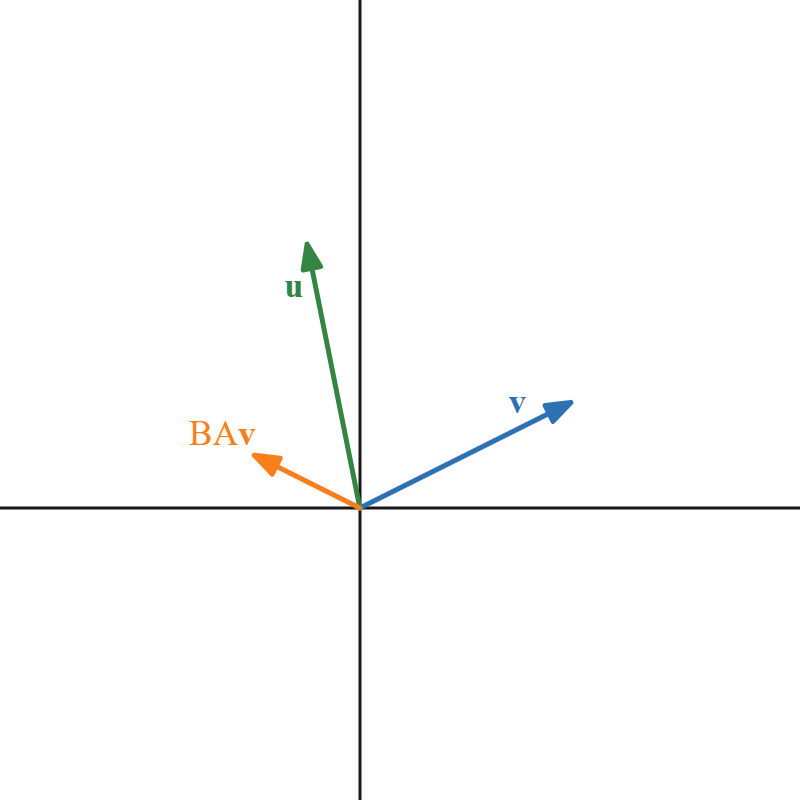
\includegraphics[width=0.5\linewidth]{chapters/chapter 3/viz matrix mult.png}
\end{figure}

Եթե $\vv$ վեկտորի վրա կիրառենք $A$-ն՝ $\vv$-ն կձևափոխվի, և կստանանք մի նոր վեկտոր՝ $A\vv$։ Հարմարության համար ստացվածը նշանակենք $\mathbf{u}$-ով: Եթե հիմա $\vu$-ի վրա կիրառենք $B$-ն, ապա այն կձևափոխի $\vu$-ն, և կունենանք մի նոր վեկտոր՝ $B\vu$: 

Արդյունքում ստացանք՝ 
\[
B\vu = B(A\vv) = (BA)\vv,
\]
ասել է թե՝ $BA$ մատրիցը կիրառած $\vv$ վեկտորի վրա։ Փաստորեն $B$ և $A$ գծային ձևափոխությունների (մատրիցների) արտադրյալը կիրառելը նույնն է, ինչ եթե նախ կիրառես $A$-ն, ապա $B$-ն․ 
\[
BA \; = \; \Big(\;\text{կիրառիր } A\text{-ն, ապա } B\text{-ն}\;\Big)
\]

\begin{marginfigure}    \begin{center}
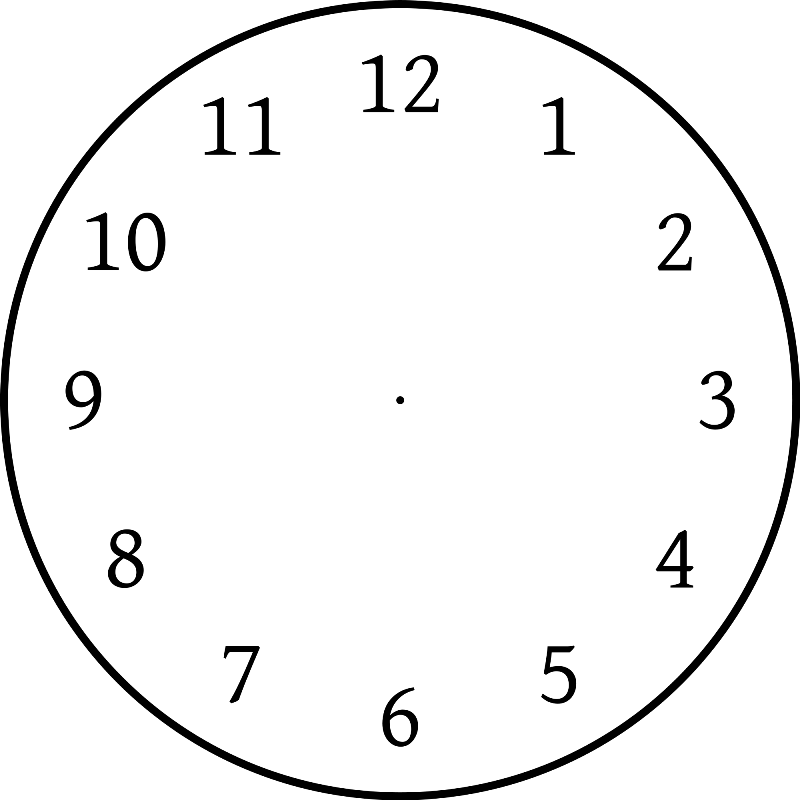
\includegraphics[width=0.55\textwidth, height=\textheight, keepaspectratio]{chapters/chapter 3/clock.png}
\end{center}
\caption*{պտույտներն ու շրջումները հարմար է պատկերացնել ժամացույցի վրա}
\end{marginfigure}

\question{Պատկերացրեք՝ $A$-ն $30^\circ$-ով պտույտն է, իսկ $B$-ն՝ ուղղաձիգի նկատմամբ հայելային արտապատկերումը (շրջումը)։ Ի՞նչ է ցույց տալիս $AB$-ն։ Իսկ $BA$՞-ն։}

Ենթադրենք $A$-ն այն մատրիցն է, որը վեկտորները պտտում է $30^\circ$-ով (ժամսլաքի ուղղությամբ),  $B$-ն՝ $50^\circ$-ով, իսկ $C$-ն՝ $260^\circ$-ով։

\question{Ի՞նչ է անում $BA$ մատրիցը։ Իսկ $CBA$՞-ն։}



\section{Միավոր մատրից}

Եթե օրինակ մատրիցը հորիզոնական ուղղությամբ $2$ անգամ ձգում է բոլոր վեկտորները՝
\[
\begin{bmatrix}
    x \\ y
\end{bmatrix}
\mapsto 
\begin{bmatrix}
    2x \\ y
\end{bmatrix}
\]
իսկ ուղղաձիգ ուղղությամբ ոչինչ չի անում, ապա  այն վեկտորները, որոնց առաջին կոորդինատը $0$ է,\marginnote{$x$-երի առանցքի վրայի վեկտորները} ձևափոխության արդյունքում չեն փոփոխվում։

Իսկ ո՞ր մատրիցն է, որ բոլոր վեկտորները թողնում է իրենց տեղերում, ոչ մեկին չի փոփոխում։ Փորձենք պարզել։

\begin{definition}
$A$-ն կոչվում է \textbf{քառակուսային} մատրից, եթե նրա տողերի ու սյուների թիվը համընկնում է։\marginnote{$n\times n$ չափանի}
\end{definition}

\begin{definition}
$A$ քառակուսային մատրիցը կոչվում է \textbf{սիմետրիկ} (համաչափ), եթե $A^T=A$:\marginnote{շրջելուց հետո մնում է նույնը}
\end{definition}

\begin{example} 
Հետևյալ մատրիցը սիմետրիկ է (ուստի և քառակուսային)՝
\[
A = \begin{bmatrix}
2 & 0 & 1 \\
0 & -3 & 4 \\
1 & 4 & 6 \\
\end{bmatrix}
\]
\end{example}

Եթե մտովի գիծ տանենք $A$ մատրիցի վերևի ձախ անկյունից դեպի ներքևի աջ անկյունը, կստանանք նրա \textit{գլխավոր անկյունագիծը,} որի նկատմամբ $A$-ն սիմետրիկ է․ $0$-ի համաչափը $0$-ն է, $1$-ի համաչափը՝ $1$-ը, և այլն։

\begin{definition}
$A$ մատրիցի \textbf{գլխավոր անկյունագիծ} (կամ պարզապես \textbf{անկյունագիծ}) ենք անվանում նրա $a_{ii}$ տեսքի տարրերը, որոնց տողերի ու սյուների համարները\marginnote{$A$-ն կարող է չլինել քառակուսային} համընկնում են՝  $a_{11}$, $a_{22}$, $\dots$:
\end{definition}

Մյուս անկյունագիծը՝ վերևի աջ անկյունից դեպի ներքևի ձախ, կոչվում է \textit{երկրորդ անկյունագիծ։}

\begin{example}
Այստեղ կարմիրով նշված է գլխավոր անկյունագիծը՝
\[
{\displaystyle {\begin{bmatrix}\color {red}{1}&0&0\\0&\color {red}{1}&0\\0&0&\color {red}{1}\end{bmatrix}}\qquad {\begin{bmatrix}\color {red}{1}&0&0&0\\0&\color {red}{1}&0&0\\0&0&\color {red}{1}&0\end{bmatrix}}\qquad {\begin{bmatrix}\color {red}{1}&0&0\\0&\color {red}{1}&0\\0&0&\color {red}{1}\\0&0&0\end{bmatrix}}\qquad {\begin{bmatrix}\color {red}{1}&0&0&0\\0&\color {red}{1}&0&0\\0&0&\color {red}{1}&0\\0&0&0&\color {red}{1}\end{bmatrix}}}
\]
իսկ այստեղ՝ երկրորդ անկյունագիծը․
\[
{\displaystyle {\begin{bmatrix}0&0&\color {red}{1}\\0&\color {red}{1}&0\\\color {red}{1}&0&0\end{bmatrix}}}
\]
\end{example}

Վերադառնանք մեր հարցին․ ո՞ր մատրիցով բազմապատկելիս է ամեն բան մնում իր տեղում։

\begin{definition}
$n$-չափանի \textbf{միավոր մատրից} է կոչվում այն քառակուսային մատրիցը\marginnote{կասենք՝ \textit{նույնական ձևափոխություն}}, որի անկյունագծի վրա $1$-եր են, իսկ մնացած բոլոր տեղերում՝ $0$-ներ։
\end{definition}

$n$-չափանի միավոր մատրիցը կարճ կնշանակենք $I_n$-ով։

\begin{example}
\[
I_3 = \begin{bmatrix}
1 & 0 &0  \\
0 & 1 &0\\
0 &0& 1\\
\end{bmatrix}
\]
\end{example}

Դժվար չէ ապացուցել, որ միավոր մատրիցով բազմապատկելիս վեկտորները չեն փոխվում՝
\[
I_n \vv = \vv \qquad \text{եթե }\vv\in\R^n
\]

Եվ ավելին, ցանկացած $A\in\R^{m\times n}$ մատրիցի և միավոր մատրիցի արտադրյալը ինքը՝ $A$-ն է․
\[ I_m A = A = A I_n \]

\question{Ի՞նչ են նշանակում $I_mA$ և $AI_n$ արտադրյալները։}



\section{Հակադարձ}

\question{Անին իր հասակը բազմապատկեց $4$-ով, հանեց $15$, բաժանեց $13$-ի և ստացավ $53$ սմ։ Որքա՞ն է Անիի հասակը։}

Պատասխանը գտնելու համար քայլերը կանենք հակառակ հերթակա\-նու\-թյամբ՝ $53$-ը կբազմապատկենք $13$-ով, կգումարենք $15$ և կբաժանենք $4$-ի, արդյունքում կստանանք Անիի հասակը։ 

Իսկ ի՞նչ, եթե ունենք մի $\vv\in \R^n$ անհայտ վեկտոր, որը ինչ-որ $A$ մատրիցով ենթարկվել է գծային ձևափոխության։ Ինչպե՞ս ունենալով $A\vv$-ն՝ վերականգնենք սկզբնական $\vv$ վեկտորը։

\begin{figure}[h]
\centering
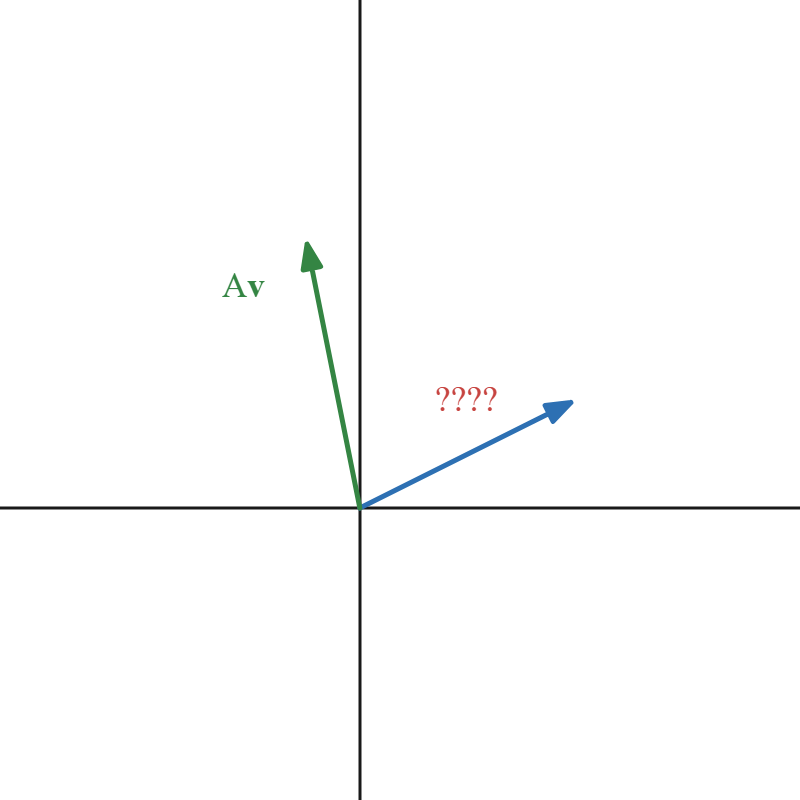
\includegraphics[width=0.5\linewidth]{chapters/chapter 3/inv.png}
\end{figure}

Այլ կերպ ասած՝ ունենալով $A$ մատրիցը, ինչո՞վ բազմապատկել $A\vv$ վեկտորը, որպեսզի ստացվի $\vv$։ Կամ՝
\[
\textbf{ի՞նչ} \; \times  \; A \; =\; I 
\]
Այդ \marginnote{$I$ ասելով նկատի ունենք համա\-պա\-տաս\-խան չափի միավոր մատրիցը} անհայտ ձևափոխությունը անվանում ենք $A$ գծային ձևափոխու\-թյան (կամ մատրիցի) \textit{հակադարձ} և նշանակում $A^{-1}$-ով։

\begin{definition}
Տրված $A$ մատրիցի \textbf{հակադարձ} կանվանենք այն $A^{-1}$ մատրիցը, որի համար
\[
AA^{-1} = A^{-1}A = I
\]
\end{definition}

Եթե գտնենք $A^{-1}$-ը, ապա կկիրառենք այն մեր ունեցած $A\vv$-ի վրա և կստանանք՝ $A^{-1}(A\vv) = (A^{-1}A)\vv=I\vv =\vv$:


\question{$A \in \R^{2 \times 2}$ գծային ձևափոխությունը վերցնում է վեկտորը և
\begin{enumerate}
    \item հորիզոնական ուղղությամբ ձգում $2$ անգամ,
    \item ապա $30^\circ$-ով պտտում,
    \item ապա ուղղաձիգ ուղղությամբ սեղմում $3$ անգամ,
    \item ապա ստացվածը շրջում $x$-երի առանցքի նկատմամբ։
\end{enumerate}
Հնարավո՞ր է ունենալով $\mathbf{v}=A\mathbf{u}$-ն՝ գտնել $\mathbf{u}$-ն։}

Պատասխանն է՝ այո, այսինքն՝ $A$ մատրիցն ունի հակադարձ (\textit{հակա\-դար\-ձելի} է)։ Ինչպես կտեսնենք, միայն որոշ քառակուսային մատրիցներ ունեն հակադարձ։

\question{Հակոբն իր հասակին գումարեց $6$, բազմապատկեց $0$-ով, հանեց $18$ և ստացավ $-18$ սմ։ Կարո՞ղ եք գտնել Հակոբի հասակը։}


\section{Որոշիչ}

Բնականաբար, հարց է առաջանում․ իսկ ինչպե՞ս գտնել տրված ձևա\-փոխու\-թյան հակադարձը, կամ առհասարակ ինչպե՞ս պարզել՝ այն ունի հակադարձ, թե ոչ։ 

Այդ նպատակով հետազոտենք մի այսպիսի տարօրինակ օբյեկտ։

\begin{definition}
\(2 \times 2\) չափանի
\[
  A = \begin{bmatrix}
    a & b \\
    c & d \\
  \end{bmatrix}
\]
մատրիցի \textbf{որոշիչ} կանվանենք\marginnote{անգլերեն՝ {\it determinant}} հետևյալ թիվը՝
\[
  \det(A) = ad - bc
\]
\end{definition}

\begin{example}
\[
  A = \begin{bmatrix}
    2 & 5 \\
    -3 & 4 \\
  \end{bmatrix}
\]
մատրիցի որոշիչն է՝ 
\[\det(A) = 2 \cdot 4 - 5 \cdot (-3) = 8+15=23\]
\end{example}

Փոքր-ինչ ավելի բարդ բանաձևով նաև $3 \times 3$ մատրիցի համար՝

\begin{definition}
\(3 \times 3\) չափանի
\begin{marginfigure}    \begin{center}

\includegraphics[width=\textwidth, height=\textheight, keepaspectratio]{chapters/chapter 3/det.png}
\end{center}
\end{marginfigure}\[
  A = \begin{bmatrix}
    a & b & c \\
    d & e & f \\
    g & h & i \\
  \end{bmatrix}
\]
մատրիցի որոշիչ կանվանենք հետևյալ թիվը՝
\[
  \det(A) = aei + bfg + cdh - ceg - bdi - afh
\]
\end{definition}

\begin{figure}[t]
\caption*{ձեռքով հաշվելիս հարմար է աջից արտագրել մատրիցի առաջին երկու սյուները, ապա հաշվել այսպես \bigskip }
\centering    {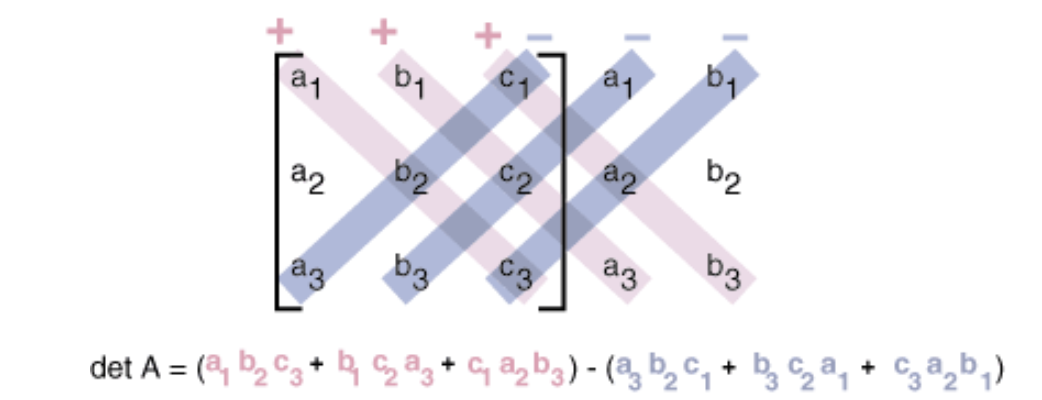
\includegraphics[width=0.8\linewidth]{chapters/chapter 3/det trick.png} }
\end{figure}

\begin{example}
\[
  A = \begin{bmatrix}
    1 & 2 & 3 \\
    4 & 5 & 6 \\
    7 & 8 & 9 \\
  \end{bmatrix}
\]
մատրիցի որոշիչն է՝ 
\[
  \det(A) = 1\cdot5 \cdot 9 + 2\cdot6\cdot7 + 3\cdot4\cdot8-3\cdot5\cdot7-2\cdot4\cdot9-1\cdot6\cdot8= 0
\]
\end{example}

Այսքանի վրա կանգ առնենք։ Ի՞նչ են ցույց տալիս այս բանաձևերը, ի՞նչ է նշանակում մատրիցի/ձևափոխության որոշիչը։

Դիտարկենք մեր $\R^2$ հարթությունը։ $x$-երի առանցքի վրա վերցնենք  \marginnote{միավոր $=$ $1$ երկարությամբ} $\ve_1=\begin{bmatrix}
    1 & 0
\end{bmatrix}$ միավոր վեկտորը, իսկ $y$-ների առանցքի վրա՝ $\ve_2=\begin{bmatrix}
    0 & 1
\end{bmatrix}$ միավոր վեկտորը։ Դրանցով կազմված փոքրիկ քառակուսին կանվանենք \textit{միավոր քառակուսի։}

\begin{figure}[h]
    \centering
    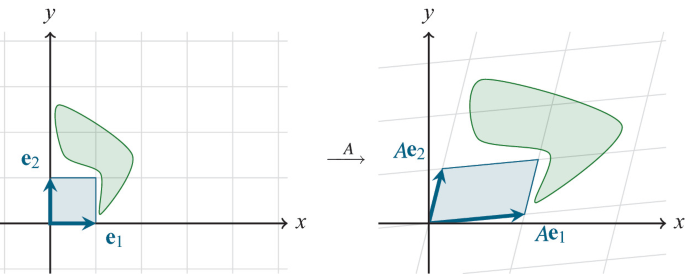
\includegraphics[width=0.75\linewidth]{chapters/chapter 3/viz area.png}
\end{figure}

$A$ ձևափոխությունը կիրառելուց հետո $\ve_1$-ն ու $\ve_2$-ը պտտվելով-ձգվելով վերածվում են $A\ve_1$ և $A\ve_2$ վեկտորների։ Քանի որ միավոր քառակուսին կազմված էր այդ երկու վեկտորներով, ապա այն նույնպես ձևափոխվում է (պտտվում-ձգվում և այլն) ու դառնում արդեն $A\e_1$ և $A\e_2$ վեկտորներով ստացվող \textit{զուգահեռագիծ։}

Եթե ձևափոխությունից առաջ միավոր քառակուսու մակերեսը $1$ էր, ապա ձևափոխությունից հետո ստացված զուգահեռագծի մակերեսը $|\det(A)|$ է։ Ավելին, ոչ միայն միավոր քառակուսու, այլ \textit{ցանկացած} պատկերի դեպքում՝ երբ կիրառում ենք $A$ ձևափոխությունը\marginnote{մտքում պատկերացրեք կետերի շարժը}, այն փոփոխվում է, իսկ նրա մակերեսը մեծանում/փոքրանում է $|\det(A)|$ անգամ։

Այսինքն՝ յուրաքանչյուր գծային ձևափոխություն կիրառելիս պատկերների մակերեսները որոշ չափով ձգվում կամ սեղմվում են, և նրա որոշիչը ցույց է տալիս, \marginnote{փաստորեն օրինակ՝ \hyperref[mona]{\color{OliveGreen} $M$ ձևափոխության արդյունքում} Մոնա Լիզան մեծանում է $\det(M)=1.89$ անգամ}\textit{թե քանի անգամ են մակերեսները ձգվում․} որոշիչը հենց այդ ձգման գործակիցն է (անգլերեն՝ {\it scaling factor})։ 

\question{Որքա՞ն է $I_n$ նույնական ձևափոխության որոշիչը։}

Արդեն իմանալով որոշիչի իմաստը՝ ձևակերպենք դրա հատկությունները։

\begin{theorem}
Ցանկացած $n \times n$ չափանի  $A$, $B$ մատրիցների համար

\begin{enumerate}
\item $\det(cA) = c^n \cdot \det(A)$ ցանկացած $c\in\R$ թվի համար\marginnote{$n$-ը մատրիցի չափն է} 

\item $\det(AB) = \det(A) \cdot \det(B)$ 

\item եթե $A$-ն ունի հակադարձ, ապա $\det(A^{-1}) = \dfrac{1}{\det(A)}$

\item $\det(I)=1$

\item $\det(A^T) = \det(A)$

\item եթե $A$-ի տողերից/սյուներից որևէ մեկը բաղկացած է միայն $0$-ներից, ապա $\det(A)=0$

\item եթե $\det (A) <0$, ապա $A$-ն նաև շրջում է տարածությունը։
\end{enumerate}
\end{theorem}

\question{Ինչո՞ւ են ճիշտ 1-4 հատկությունները։}

Նշենք, որ $4 \times 4$, $5 \times 5$ և ավելի մեծ չափանի քառակուսային մատրիցների որոշիչները հաշվելու համար նույնպես կան տարբեր բանաձևեր (իսկ ոչ քառակուսային մատրիցները \textbf{որոշիչ չունեն}), բայց դրանց հաշվողական մասը մեզ հետաքրքիր չէ։ Օգտակար կլինի նաև իմանալ, որ
\begin{theorem}
Եթե մատրիցի տողերից կամ սյուներից որևէ մեկը
\begin{itemize}
\item բազմապատկենք ինչ-որ $c$ թվով, ապա որոշիչը կմեծանա $c$ անգամ,

\item գումարենք որևէ այլ տողի/սյան, ապա որոշիչը չի փոխվի։
\end{itemize}
\end{theorem}

\section{Հակադարձելիություն}

Իսկ ի՞նչ, եթե գծային ձևափոխության որոշիչը $0$ է։

\begin{figure}[h]
    \centering
    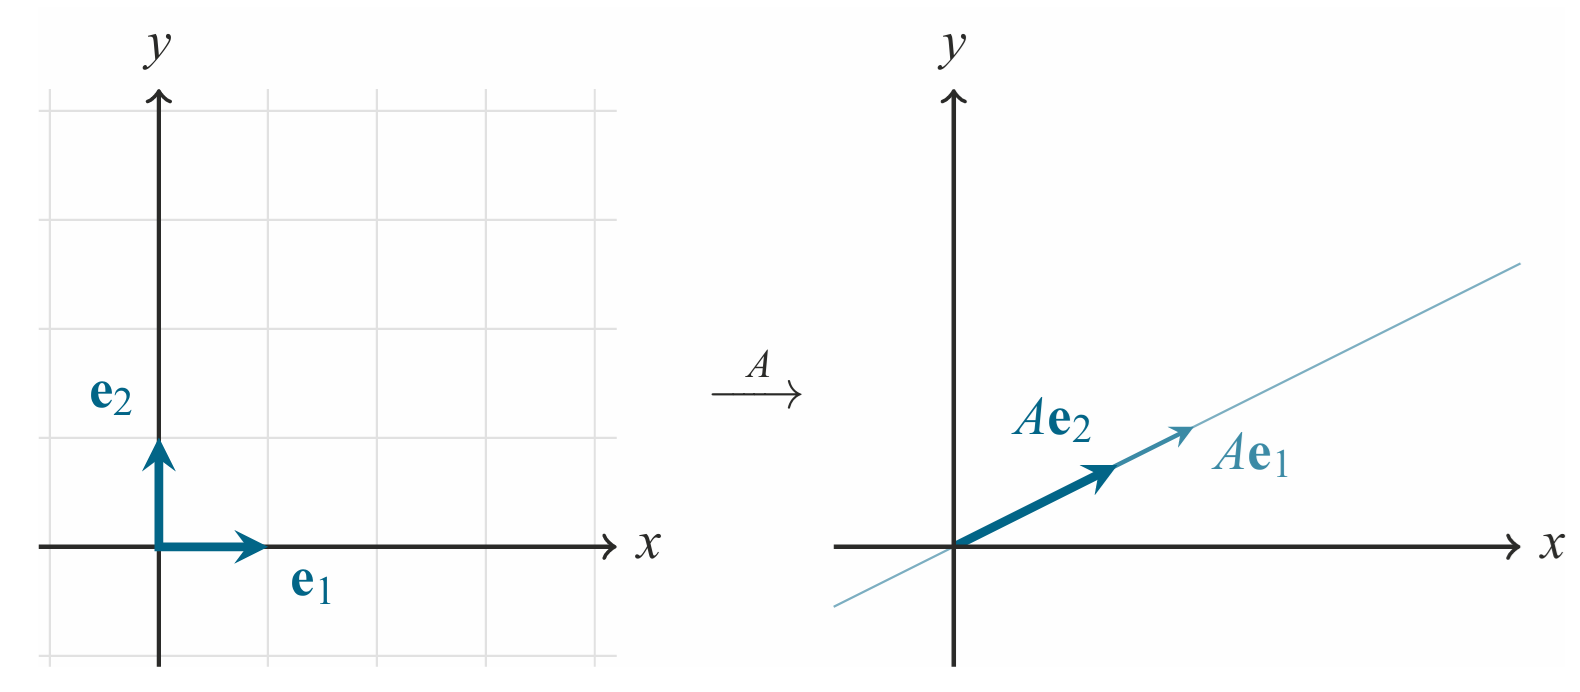
\includegraphics[width=0.75\linewidth]{chapters/chapter 3/0 det.png}
\end{figure}

Նշանակում է՝ ցանկացած պատկերի մակերեսը ձևափոխությունից հետո դառնում է $0$։ Այսինքն ձևափոխությունը տարածության մեջ եղած ամեն ինչ սեղմում-ճզմում է՝ դարձնելով զրո մակերեսով ինչ-որ բան\marginnote{$\R^3$-ի դեպքում՝ նաև հարթություն} ($\R^2$-ի դեպքում՝ ուղիղ կամ պարզապես կետ)։

\question{$A$ մատրիցը յուրաքանչյուր $[x \quad y]$ վեկտորի տանում է դեպի $[x \quad 0]$։ Ո՞ր վեկտորները $A$-ն կիրառելիս կդառնան $[7 \quad 0]$:}  
Այս դեպքում եթե վերցնենք որևէ $\vv$ վեկտոր, կիրառենք $A$-ն (ճզմելով տարածությունը) և փորձենք $A\vv$-ից հետ գնալ դեպի սկզբնական $\vv$ վեկտորը, ապա որքան էլ ուզենք՝ չենք կարող պարզել, թե որն էր $\vv$-ն, քանի որ $\vv$-ի հետ նույն գծի վրա գտնվող բազմաթիվ այլ վեկտորներ ևս ճզմվելով դարձել են $A\vv$։

\begin{theorem}
$A$ քառակուսային\marginnote{ոչ քառակուսային մատրիցները ևս հակադարձ չունեն} մատրիցն ունի հակադարձ այն և միայն այն դեպքում, եթե $\det(A) \ne 0$:
\end{theorem}

Ինչպես կարող ենք ստուգել, $2 \times 2$ չափանի 
\[
\begin{bmatrix}
    a & b \\ c & d
\end{bmatrix}
\]
մատրիցի հակադարձը (եթե $\det(A)\ne 0$) կարելի է գտնել հետևյալ բանաձևով՝\marginnote{ստուգեք, որ $AA^{-1}=I_2$}
\[
A^{-1} = \frac{1}{\det(A)} \begin{bmatrix} d & -b \\ -c & a \end{bmatrix}
\]

\begin{example}
$A = \begin{bmatrix} 2 & 3 \\ 1 & 4 \end{bmatrix}$ մատրիցը հակադարձելի է և
\[
A^{-1} = \frac{1}{\det A} \begin{bmatrix} 4 & -3 \\ -1 & 2 \end{bmatrix} = \frac{1}{5} \begin{bmatrix} 4 & -3 \\ -1 & 2 \end{bmatrix}=\begin{bmatrix}
    0.8 & -0.6 \\ -0.2 & 0.4
\end{bmatrix}
\]
\end{example}

\question{Սկզբից կիրառել ենք $A$ ձևափոխությունը, այնուհետև $B$-ն, և ստացել ենք $\vu$։ Ինչպե՞ս գտնենք սկզբնական վեկտորը։}

Ավելի մեծ չափանի հակադարձները հաշվելու համար նույնպես կան բավական հետաքրքիր բանաձևեր և ալգորիթմներ, բայց մենք դրանց նույնպես ուշադրություն չենք դարձնի։ Նկատենք միայն, որ
\[
\left(AB\right)^{-1} = B^{-1}A^{-1}
\]

\section{Հետք}

Որոշիչից բացի սահմանենք նաև մատրիցի հետքը։

\begin{definition}
$A$ քառակուսային մատրիցի \textbf{հետք} կանվանենք նրա անկյունագծի վրա գրված տարրերի գումարը՝\marginnote{անգլերեն՝ {\it trace}}
\[
\operatorname{tr}(A) = a_{11} + a_{22} + \ldots + a_{nn}
\]
\end{definition}

\begin{example}
\[
  A = \begin{bmatrix}
    2 & 5 & 1 \\
    0 & -3 & 4 \\
    7 & 2 & 6 \\
  \end{bmatrix}
\]
մատրիցի հետքն է՝
\[
  \operatorname{tr}(A) = 2 + (-3) + 6 = 5
\]
\end{example}

Ի՞նչ է ցույց տալիս հետքը։ Այս մասին կխոսենք ավելի ուշ։ Առայժմ ֆիքսենք դրա հատկությունները։

\begin{theorem}
Ցանկացած $n \times n$ չափանի  $A$, $B$ մատրիցների համար

\begin{enumerate}
\item \(\operatorname{tr}(cA) = c \cdot \operatorname{tr}(A)\) ցանկացած $c\in \R$ թվի համար

\item \(\operatorname{tr}(A + B) = \operatorname{tr}(A) + \operatorname{tr}(B)\)

\item \(\operatorname{tr}(AB) = \operatorname{tr}(BA)\) 

\item \(\operatorname{tr}(A^T) = \operatorname{tr}(A)\)
\end{enumerate}
\end{theorem}

Ինչպես տեսնում ենք, մատրիցի հետքը հարուստ է շատ օգտակար հատկություններով։ Ինչ-որ իմաստով՝ նրա սահմանումը միակն է, որ կարող է բավարարել բոլոր վերոնշյալ $4$ հատկություններին։



\bigskip 

\begin{theory}
.
\begin{itemize}
\item կարդալ [{\rm Poole}], 221-223 էջերը (ձևափոխության հակադարձ)
\item կարդալ [{\rm Johnston}], 254-256 (հետք), 258-263 (որոշիչ) էջերը  
\item դիտել  {\rm 3b1b}-ի \href{https://www.3blue1brown.com/lessons/matrix-multiplication}{4-րդ} և \href{https://www.3blue1brown.com/lessons/determinant}{6-րդ} տեսադասերը գծային հանրահաշվից 
\item ըստ ցանկության՝ նաև \href{https://www.3blue1brown.com/lessons/inverse-matrices}{7-րդը}
\item տեսնել որոշ մատրիցներ \href{https://intuitive-math.club/linear-algebra/matrices}{սեփական աչքով}
\end{itemize}
\end{theory}

\newpage

\section{Խնդիրներ}

\begin{problem}
Ձևափոխության նկարագրությունը համապատասխանեցրեք իր մատրիցին․ 

\textit{Նկարագրություն՝} 

\begin{enumerate}[label={\alph*}․]
\item պտտում է $70^\circ$-ով
\item ոչինչ չի անում
\item շրջում է $x$-երի առանցքի շուրջ
\item $y$-ների ուղղությամբ ձգում է $5$ անգամ
\item ամեն բան տանում է $y=6x$ ուղղի վրա
\item ամեն բան տանում է $y=6x+1$ ուղղի վրա
\end{enumerate}

\setlength{\columnseprule}{0pt}

\textit{Մատրից՝} 
\begin{multicols}{2}
\begin{enumerate}
\item $\begin{bmatrix}
    1&0\\0&5
\end{bmatrix}$\vfill
\item այդպիսի մատրից չկա\vfill
\item $\begin{bmatrix}
    1&0\\0&1
\end{bmatrix}$
\item $\begin{bmatrix}
    0.342 & -0.939\\
     0.939& 0.342
\end{bmatrix}$
\item $\begin{bmatrix}
    1&0\\0&-1
\end{bmatrix}$
\item $\begin{bmatrix}
    3&-1\\18&-6
\end{bmatrix}$
\end{enumerate}
\end{multicols}


\hint{Հաշվեք որոշիչները։ Հետևեք նաև, թե ո՞ւր է գնում $\mathbf{0}$-ն։}
\end{problem}

\begin{problem}
Ինչի՞ է հավասար մատրիցի որոշիչը, եթե այն
    
\begin{enumerate}[label={\alph*}․]
\item ամեն ինչ պտտում է $14^\circ$-ով և $1.5$ անգամ ձգում $x$-երի ուղղությամբ

\item \textit{ա․} մատրիցի հակադարձն է

\item $\begin{bmatrix}
    1 & 0
\end{bmatrix}$ վեկտորը տանում է $\begin{bmatrix}
    2 & 4
\end{bmatrix}$, իսկ $\begin{bmatrix}
    0 & 1
\end{bmatrix}$-ը՝ $\begin{bmatrix}
    -1 & 0
\end{bmatrix}$

\item ունի հետևյալ տեսքը՝ $\begin{bmatrix}
2 & 3 \\ 2 &1
\end{bmatrix}$

\item ունի հետևյալ տեսքը՝ $\begin{bmatrix}
8&3&5\\1&4&2\\-4&0&4   \end{bmatrix}$

\item \textit{ե․} մատրիցն է՝ բարձրացրած խորանարդ
\end{enumerate}
\end{problem}


\begin{problem}
Եթե վերցնենք $x^2+y^2=1$ միավոր շրջանագիծը և $2$ անգամ ձգենք $x$-երի առանցքի ուղղությամբ,\marginnote{$(0,0)$ կենտրոնով և $1$ շառավղով} արդյունքում կստանանք \textit{էլիպս։} Որքա՞ն կլինի դրա մակերեսը։

\begin{figure}[!h]
    \centering
    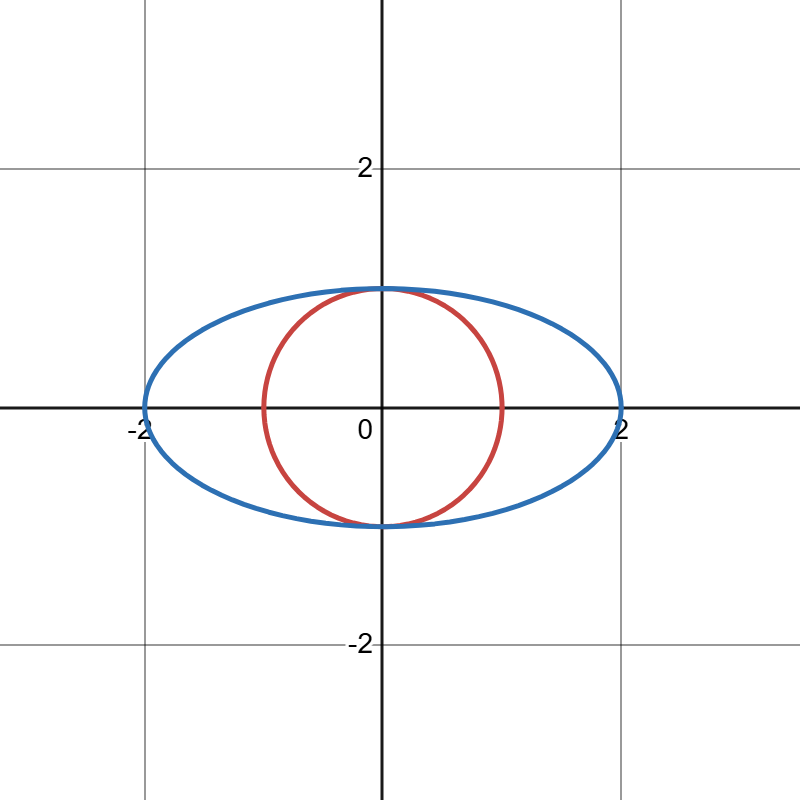
\includegraphics[width=0.45\linewidth]{chapters/chapter 3/ellipse.png}
\end{figure}

Կարո՞ղ եք ընդհանրացնելով արդյունքը՝ ստանալ բանաձև էլիպսի մակերեսի համար։
\end{problem}


\begin{problem}
Հայտնի է, որ
\[
A=\begin{bmatrix}
    4 & -8 \\ 1 & 2
\end{bmatrix}
\]
մատրիցը ինչ-որ $\mathbf{v}$ վեկտորի տանում է դեպի
\begin{enumerate}[label={\alph*}․]
\item $\begin{bmatrix}
    1 \\2
\end{bmatrix}$
\item $\begin{bmatrix}
    3 \\ 4
\end{bmatrix}$
\end{enumerate}
Կարո՞ղ եք գտնել $\mathbf{v}$ վեկտորը։
\end{problem}

\begin{problem}
Ենթադրենք տրված է 
\[
A=\begin{bmatrix}
    a & b \\ c & d
\end{bmatrix}
\]
\begin{marginfigure}
    \caption*{այս գծագիրը կարող է օգնել}
    \centering
    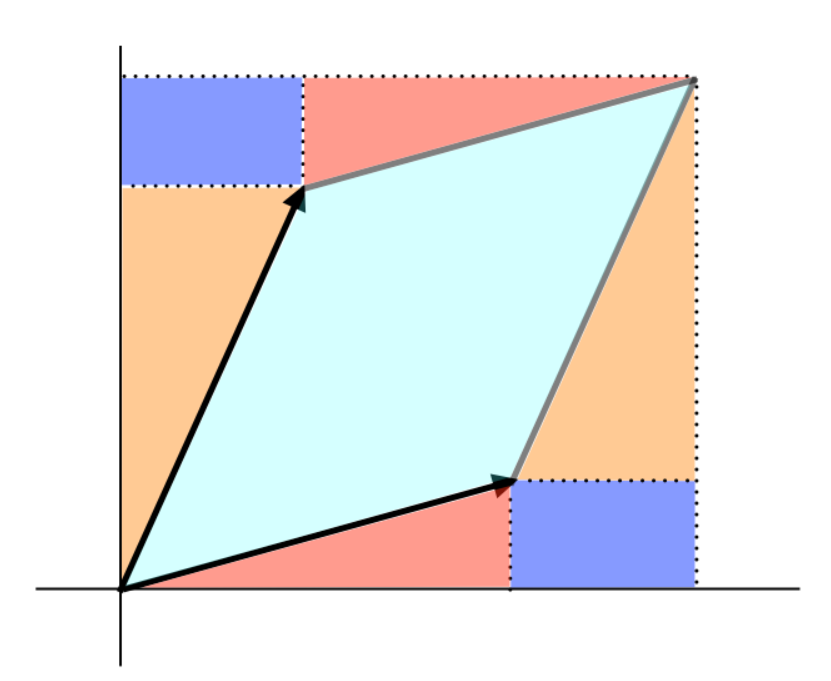
\includegraphics[width=\linewidth]{chapters/chapter 3/det explained.png}
\end{marginfigure}
մատրիցը։ $A$-ն կիրառելիս 
\begin{enumerate}[label={\alph*}․]
\item որտե՞ղ է գնում $\begin{bmatrix}
    1 & 0
\end{bmatrix}$ վեկտորը

\item որտե՞ղ է գնում $\begin{bmatrix}
    0 & 1
\end{bmatrix}$ վեկտորը

\item ինչո՞ւ է դրանցով ստացված զուգահեռագծի մակերեսը հավասար $|\det(A)|$-ին
\end{enumerate}
\end{problem}


\begin{problem}
Ինչպես գիտենք, ցանկացած մատրից միավոր մատրիցով բազմապատկելիս մնում է նույնը։ Տեղերով փոխենք $I_4$ մատրիցի երկրորդ և երրորդ տողերը՝
\[
B = \begin{bmatrix}
    1 & 0 & 0 & 0 \\
    0 & 0 & 1 & 0 \\
    0 & 1 & 0 & 0 \\
    0 & 0 & 0 & 1
\end{bmatrix}
\]
\begin{enumerate}[label={\alph*}․]
\item ի՞նչ է լինում $4 \times 4$ չափի մատրիցի հետ, երբ այն բազմապատկում ենք $B$-ով (ենթադրենք՝ ձախից)

\item որքա՞ն է $B$-ի որոշիչը

\item ինչպե՞ս է փոխվում մատրիցի որոշիչը, երբ նրա երկրորդ ու երրորդ տողերը տեղերով փոխում ենք

\item ինչպե՞ս կընդհանրացնեք ստացված արդյունքը
\end{enumerate}
\end{problem}

\setchapterpreamble[u]{\margintoc}
\chapter{Գծային տարածությունների կառուցվածքը}
\labch{structure}

\emergencystretch 2em

\section{Գծային թաղանթ}

Ինչո՞ւ ենք գծային տարածությունների և ձևափոխությունների մասին խոսելիս առանձնահատուկ ուշադրություն դարձնում ձախում պատկեր\-ված երկու վեկտորներին, այլ ոչ թե ասենք՝ աջ կողմի երկու վեկտորներին։

\begin{figure}[h]
    \centering
    \subfloat{{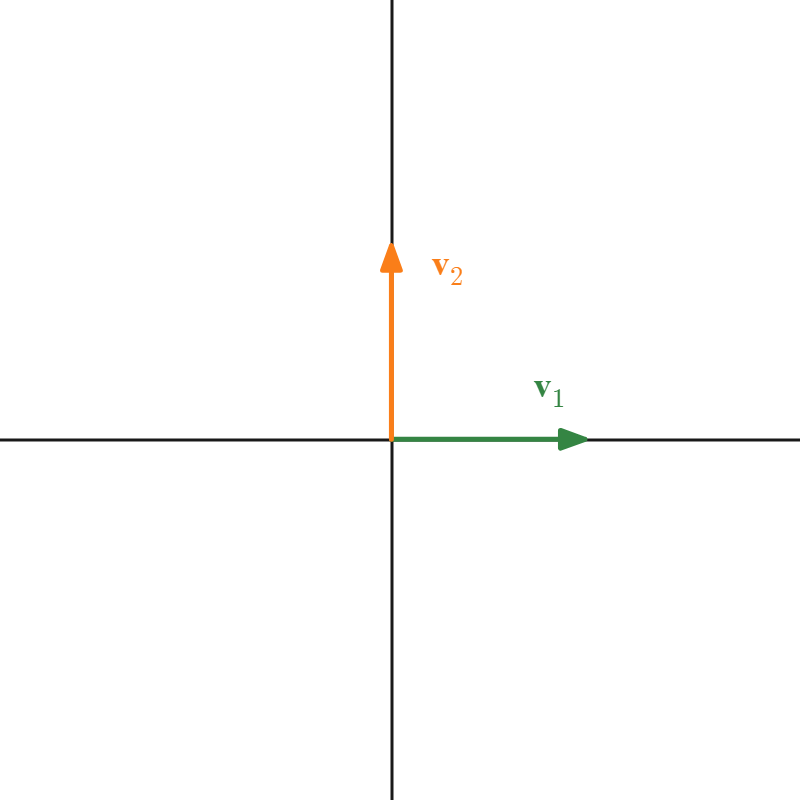
\includegraphics[width=0.4\linewidth]{chapters/chapter 4/two good vectors.png} }}%
    \qquad
    \subfloat{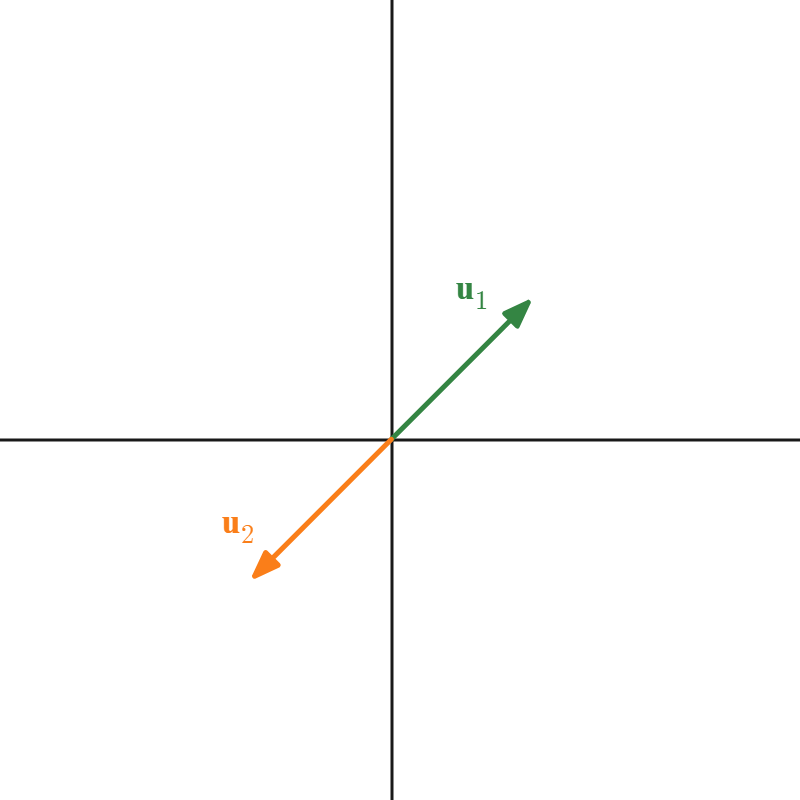
\includegraphics[width=0.4\linewidth]{chapters/chapter 4/two bad vectors.png}} %
\end{figure}

\textit{— Որովհետև ձախ կողմի երկու վեկտորներով կարելի է ստա\-նալ հարթության ցանկացած այլ վեկտոր,— }կասեք Դուք։

Իսկ ինչո՞ւ սահմանափակվել $\vv_1$, $\vv_2$-ով, ինչո՞ւ չնայել այս վեկտորներին՝

\begin{figure}[h]
    \centering
    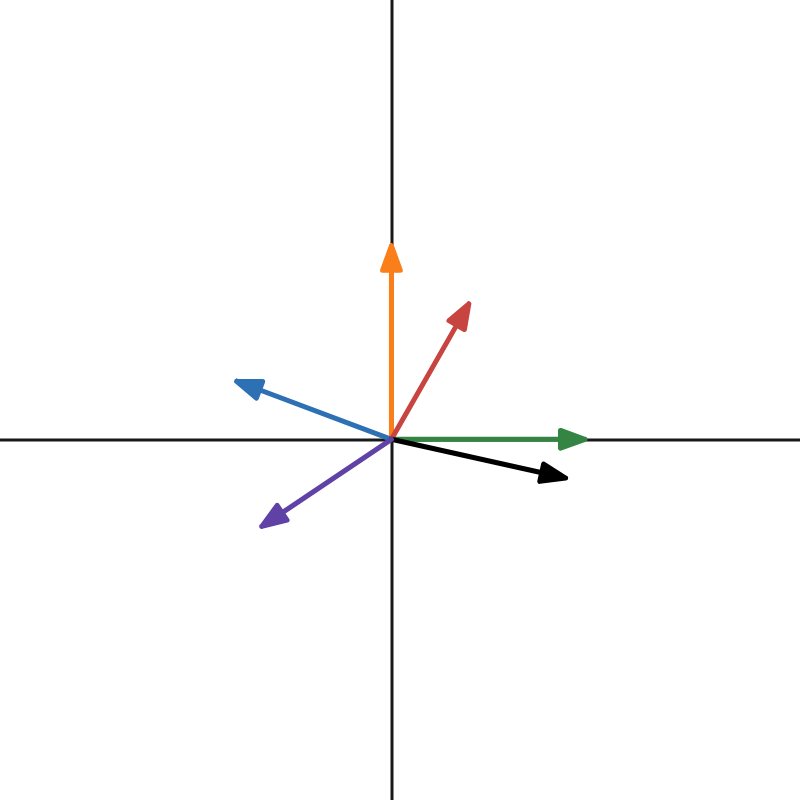
\includegraphics[width=0.4\linewidth]{chapters/chapter 4/too many vectors.png}
\end{figure}

Որովհետև սրանք արդեն չափից շատ են․ $\R^2$-ում բավարար է ունենալ երկու վեկտոր (առաջին նկարի նման), և դրանցով կարելի է ստանալ ցանկացած այլ վեկտոր։

Հստակ ձևակերպենք, թե ինչ նկատի ունենք «ցանկացած վեկտոր ստանալ» ասելով։ Եթե 
\[\vv_1=\begin{bmatrix}
    1 \\ 0
\end{bmatrix}, \qquad \vv_2=\begin{bmatrix}
    0 \\ 1
\end{bmatrix}
\]
ապա $\R^2$ տարածության յուրաքանչյուր $\vu$ վեկտոր կարող ենք գրել 
\[
\vu = (\text{ինչ-որ բան}) \cdot \vv_1 + 
(\text{ինչ-որ բան}) \cdot \vv_2
\]
տեսքով։ Օրինակ՝ $\begin{bmatrix}
    4 & -7
\end{bmatrix}$ վեկտորը կգրենք որպես՝
\[
\begin{bmatrix}
    4 \\ -7
\end{bmatrix}
= 4 \cdot \begin{bmatrix}
    1 \\ 0
\end{bmatrix}+ (-7) \cdot 
\begin{bmatrix}
    0 \\ 1
\end{bmatrix}
=  
4 \vv_1 - 7 \vv_2
\]

Այս դեպքում ասում ենք, որ $\begin{bmatrix}
    4 & -7
\end{bmatrix}$ վեկտորը $\vv_1$ և $\vv_2$ վեկտորների \textit{գծային զուգակցություն} է կամ պատկանում է $\vv_1$-ի և $\vv_2$-ի \textit{գծային թաղանթին։}

\begin{definition}
\[ 
c_1\mathbf{v}_1 + c_2\mathbf{v}_2 + \ldots + c_k\mathbf{v}_k 
\]
տեսքի ցանկացած արտահայտություն\marginnote{որտեղ $c_1$, $\ldots$, $c_k$ ցանկացած թվեր են} կանվանենք \(\mathbf{v}_1, \mathbf{v}_2, \ldots, \mathbf{v}_k\) վեկտորների \textbf{գծային զուգակցություն} (կոմբինացիա)։ 

$\vv_1$, $\vv_2$, $\dots$, $\vv_k$ վեկտորների բոլոր հնարավոր գծային զուգակցու\-թյուն\-ների բազմությունը կանվանենք այդ վեկտորների \textbf{գծային թաղանթ․}
\[
\operatorname{span}\{\vv_1, \vv_2, \ldots, \vv_k\} =    \{c_1\vv_1 + c_2\vv_2 + \ldots + c_k\vv_k \,\mid\, c_1, c_2, \ldots, c_k \in \mathbb{R}\}
\]
\end{definition}

\begin{figure}[h]
    \centering
    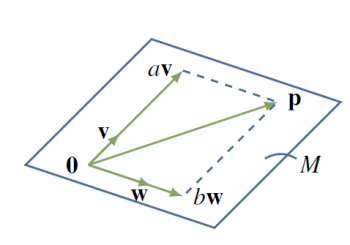
\includegraphics[width=0.5\linewidth]{chapters/chapter 4/span.png}
    \caption*{այստեղ $\mathbf{p}=a\vv+b\vw$}
\end{figure}

Երկրաչափորեն՝ $\vv_1$, $\dots$, $\vv_k$ վեկտորների գծային թաղանթը բոլոր այն վեկտորներն են, որոնք կարելի է ստանալ այդ վեկտորները ձգելով, սեղմելով և իրար գումարելով։ 

\begin{marginfigure}
% \centering
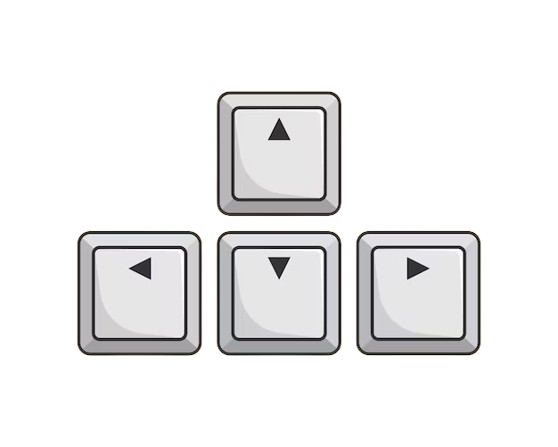
\includegraphics[width=0.8\linewidth]{chapters/chapter 4/arrow keys.png}
\end{marginfigure}

\question{Ո՞րն է $\leftarrow$, $\rightarrow$, $\uparrow$, $\downarrow$ կոճակների գծային թաղանթը։ Իսկ $\leftarrow$, $\rightarrow$ կոճակների՞նը։ Իսկ $\leftarrow$-ի՞նը։}

\begin{figure}[!h]
    \centering
    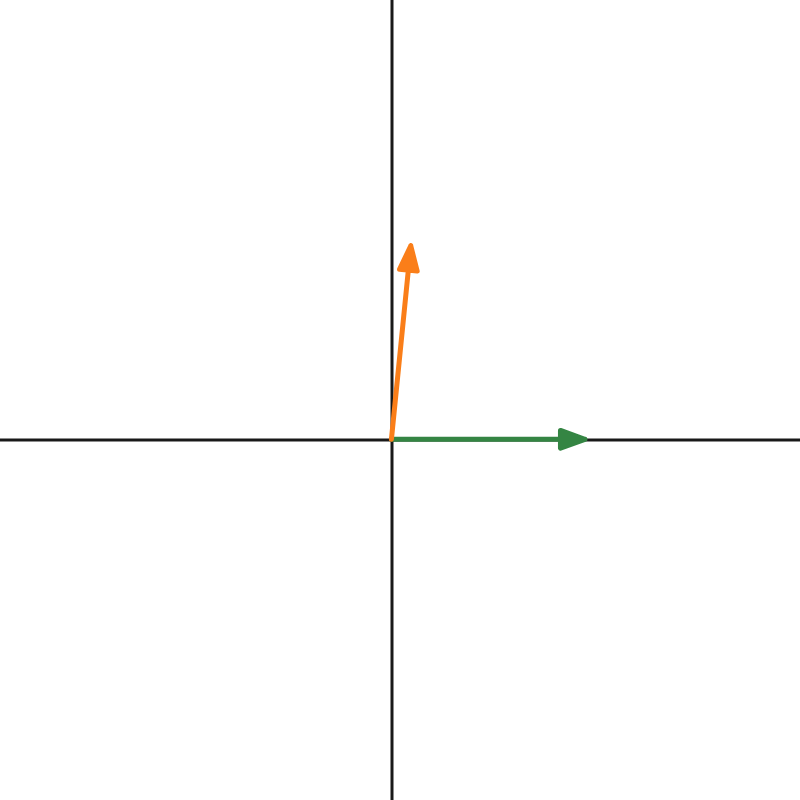
\includegraphics[width=0.4\linewidth]{chapters/chapter 4/span_1.png}
\end{figure}

\question{Հնարավո՞ր է $[4 \quad 3]$ վեկտորը արտահայտել $[1 \quad 0]$-ի և $[0.1 \quad 1]$-ի գծային զուգակցությունով։}

\begin{example}\label{2d_span}
\[
\begin{bmatrix}
    1 \\ 0
\end{bmatrix}
\qquad \text{և} \qquad 
\begin{bmatrix}
    0.1 \\ 1
\end{bmatrix}
\]
վեկտորների գծային թաղանթը կրկին $\R^2$-ն է։
\end{example}

\begin{figure}[!h]
    \centering
    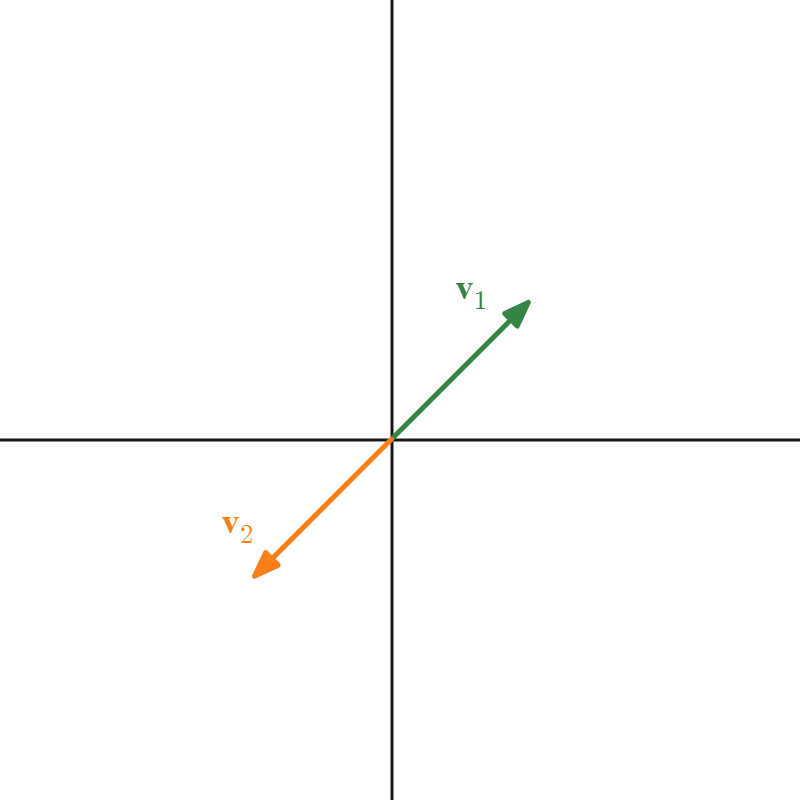
\includegraphics[width=0.4\linewidth]{chapters/chapter 4/span_2.png}
\end{figure}

\begin{example}\label{1d_span}
\[
\begin{bmatrix}
    1 \\ 1
\end{bmatrix}
\qquad \text{և} \qquad 
\begin{bmatrix}
    -1 \\ -1
\end{bmatrix}
\]
վեկտորների գծային թաղանթը $y=x$ ուղիղն է, քանի որ երկուսն էլ ընկած են այդ ուղղի վրա. հնարավոր չէ դրանք ձգելով-գումարելով ստանալ այդ ուղղից դուրս վեկտոր։
\end{example}

Ընդ որում, բավարար է վերցնել դրանցից միայն մեկը․ 


\begin{figure}[!h]
    \centering
    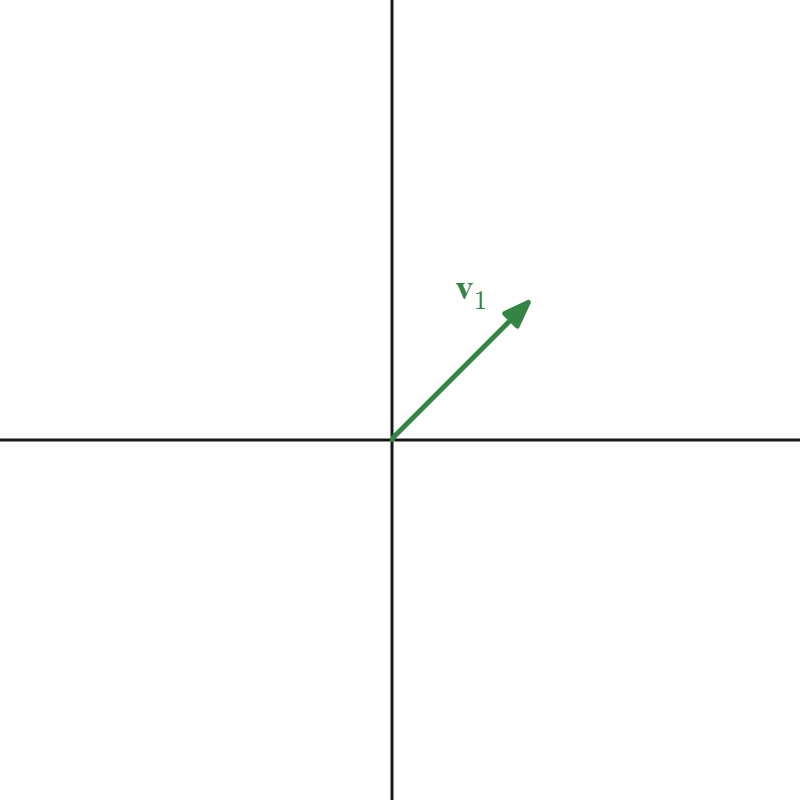
\includegraphics[width=0.4\linewidth]{chapters/chapter 4/span_3.png}
\end{figure}

\begin{example}
\[
\begin{bmatrix}
    1 \\ 1
\end{bmatrix}
\]
\marginnote{բազմապատկելով $-1$-ով՝ կստանանք $\vv_2$}վեկտորի գծային թաղանթը նույնպես $y=x$ ուղիղն է։
\end{example}

\question{Ո՞րն է $y=kx$ ուղղի վրա ընկած երկու վեկտորների  գծային թաղանթը։ Իսկ երեք վեկտորների՞։}

Նախորդ օրինակներում վեկտորների թաղանթը մի դեպքում ստացվեց հարթություն, մյուս դեպքում՝ ուղիղ։ Կարելի է ապացուցել, որ
\begin{theorem}
\marginnote{եթե վեկտորները $\R^n$-ում են, դրանց թաղանթը $\R^n$-ի ենթատարածություն է}Վեկտորների գծային թաղանթը գծային տարածու\-թյուն է։
\end{theorem}

\section{Գծորեն անկախություն}

Բայց ո՞րն է պատճառը, որ \hyperref[2d_span]{\color{OliveGreen} մի դեպքում} երկու վեկտորների գծային թաղանթը ամբողջ տարածությունն է, \hyperref[1d_span]{\color{OliveGreen} մեկ այլ դեպքում՝} ինչ-որ մի ուղիղ։ 

Տարբերությունն այն էր, որ երկրորդ դեպքում վեկտորները ընկած էին նույն ուղղի վրա, այսինքն հնարավոր էր դրանցից \textit{մեկը արտահայտել մյուսով։} Նման դեպքերում կասենք, որ վեկտորները \textit{գծորեն կախված} (կախյալ) են։

\begin{definition}
$\vv_1$, $\vv_2$, $\ldots$, $\vv_n$ վեկտորները կոչվում են \textbf{գծորեն անկախ,} եթե դրանցից ոչ մեկը հնարավոր չէ արտահայտել մյուսների գծային զուգակցության միջոցով։
\end{definition}

Եվ իհարկե, կասենք, որ վեկտորները \textbf{գծորեն կախված} են, եթե դրանցից որևէ մեկը (ասենք՝ $\vv_n$-ը) հնարավոր է արտահայտել մյուսներով՝
\[
\vv_n = c_1 \vv_1 + c_2 \vv_2 + \dots + c_{n-1}\vv_{n-1}
\]

\begin{figure}[h]
    \centering
    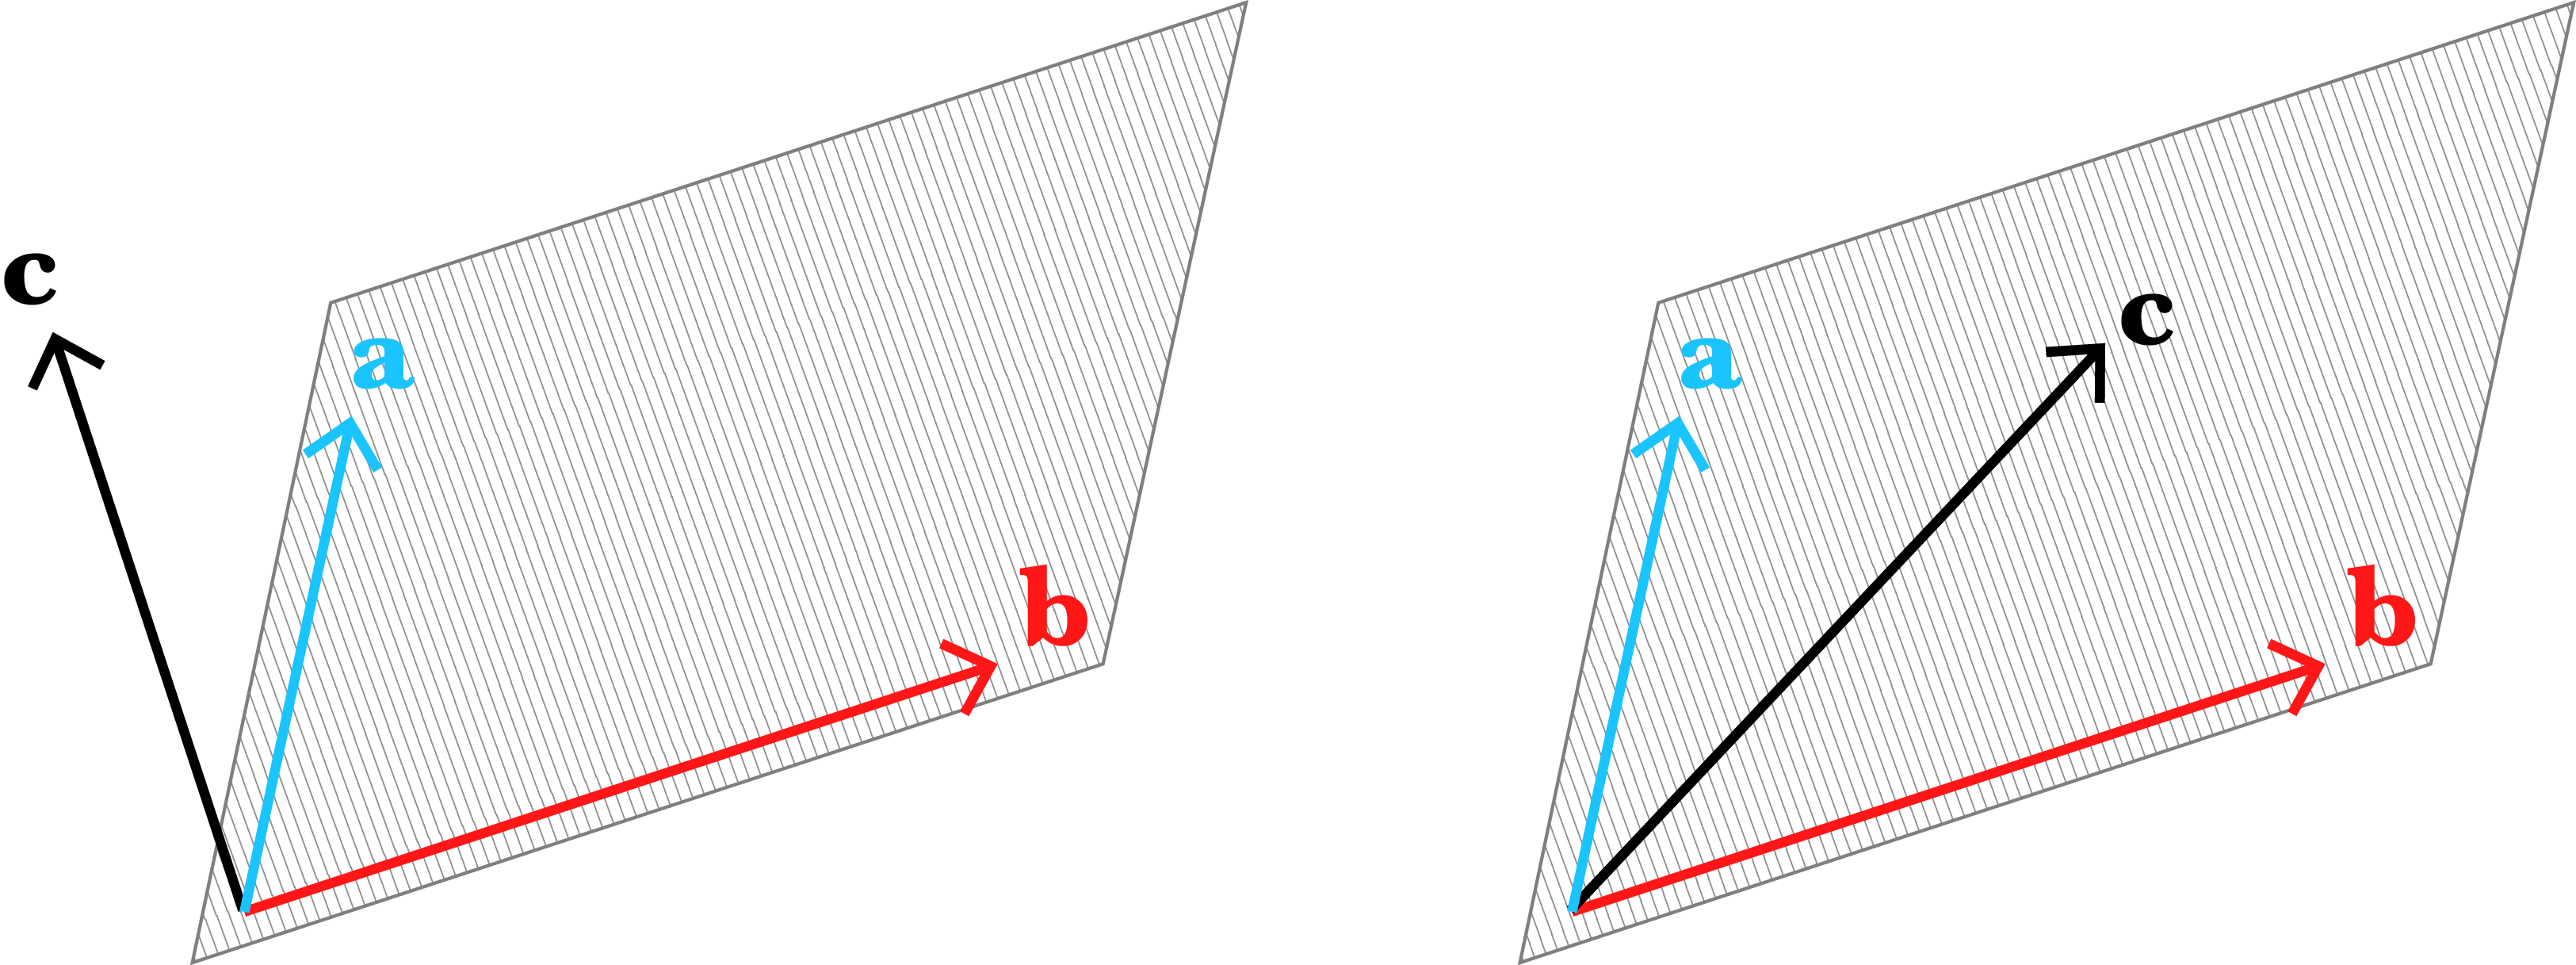
\includegraphics[width=0.85\linewidth]{chapters/chapter 4/linear-dependence-3d.png}
    \caption*{առաջին նկարում $\va$, $\vb$, $\vc$-ն գծորեն անկախ են, երկրորդում՝ ոչ}
\end{figure}


\question{Անցեք \href{https://www.desmos.com/calculator/gglf9fj10w}{հղումով} և խաղացեք $a$-ի ու $b$-ի հետ։ Ի՞նչ վեկտորներ եք ստանում։ Իսկ \href{https://www.desmos.com/calculator/1g2zq4exup}{այստե՞ղ}։}


Երկրաչափորեն,
\begin{itemize}
    \item երկու վեկտորներ գծորեն կախված են, եթե դրանք ընկած են միևնույն ուղղի վրա

    \item երեք վեկտորներ գծորեն կախված են, եթե դրանք ընկած են միևնույն հարթության մեջ
\end{itemize}
և այլն։

\question{$\vv_1$, $\vv_2$, $\vv_3$ վեկտորներից մեկը $\mathbf{0}$ է։ Կարո՞ղ են դրանք լինել գծորեն անկախ։}


Վեկտորների գծորեն անկախությունը ստուգելիս երբեմն հարմար է օգտվել հետևյալ թեորեմից (որը կարող եք ապացուցել):

\begin{theorem}
$\vv_1$, $\dots$, $\vv_n$ վեկտորները գծորեն անկախ այն և միայն այն դեպքում, եթե 
\[
\text{« } c_1\vv_1 + c_2\vv_2 + \ldots + c_n\vv_n = \mathbf{0} \text{ »}
\]
\marginnote{այսինքն՝ $0$-ից բացի ինչ թվեր էլ դնենք, գումարը $\mathbf{0}$ չի լինի}հավասարությունը տեղի ունի \textit{միմիայն} այն դեպքում, երբ $c_1 = c_2 = \ldots = c_n = 0$։
\end{theorem}


\section{Հենք}

Փաստորեն մեր
\[\vv_1=\begin{bmatrix}
    1\\0
\end{bmatrix}\qquad \text{ և }\qquad \vv_2=\begin{bmatrix}
    0\\1
\end{bmatrix}\] 
վեկտորները գծորեն անկախ են, և նրանց գծային թաղանթը ամբողջ $\R^2$-ն է։ 
Նման դեպքերում ասում ենք, որ $\vv_1$-ն ու $\vv_2$-ը կազմում են $\R^2$ տարածության \textit{հենք} կամ \textit{բազիս։}



\begin{definition}
$\vv_1$, $\vv_2$, $\dots$, $\vv_n$ վեկտորները կոչվում են $V$ գծային տարածության \textbf{հենք} (կամ \textbf{բազիս}), եթե
\begin{enumerate}
    \item $\vv_1$, $\vv_2$, $\dots$, $\vv_n$ գծորեն անկախ են, և
    
    \item $\vv_1$, $\vv_2$, $\dots$, $\vv_n$-ի գծային թաղանթը ամբողջ $V$-ն է։
\end{enumerate}
\end{definition}

Այսինքն՝ $V$-ի ցանկացած վեկտոր կարելի է արտահայտել $\vv_1$, $\dots$, $\vv_n$-ով, և դրանցից ոչ մեկն ավելորդ չէ․ եթե $\vv_i$-երից որևէ մեկը հեռացնենք, այն այլևս չի լինի հենք։

Ավելին, ցանկացած վեկտոր տվյալ հենքով կարելի է արտահայտել ուղիղ \textit{մեկ ձևով․} այսինքն օրինակ՝ $\begin{bmatrix}
    3 & 4
\end{bmatrix}$-ը $\vv_1=\begin{bmatrix}
    1 & 0
\end{bmatrix}$-ով ու $\vv_2=\begin{bmatrix}
    0 & 1
\end{bmatrix}$-ով արտահայտելու միակ ձևն է՝ $3\cdot \vv_1+4\cdot\vv_2$։

\begin{example}
\begin{marginfigure}
\centering
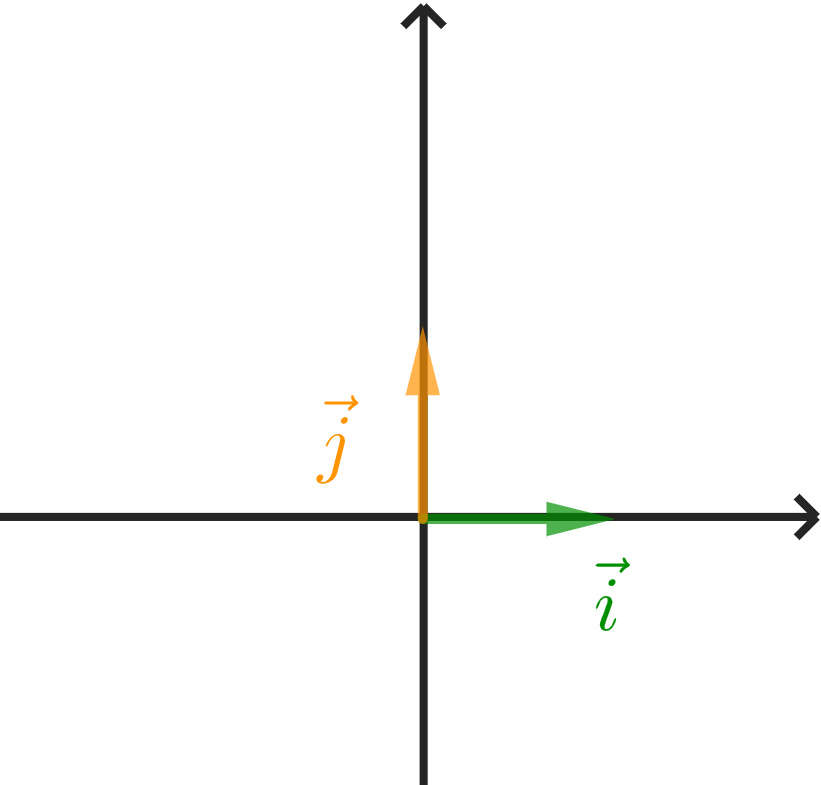
\includegraphics[width=0.6\textwidth, keepaspectratio]{chapters/chapter 4/ij basis.png}
\end{marginfigure}
\[
\mathbf{e}_1 = \begin{bmatrix} 1 \\ 0 \end{bmatrix}, \qquad \mathbf{e}_2 = \begin{bmatrix} 0 \\ 1 \end{bmatrix}
\]
վեկտորները $\mathbb{R}^2$-ի համար կազմում են հենք (կոչվում է $\R^2$-ի \textit{ստանդարտ հենք})։ Այս երկու վեկտորները հաճախ նշանակում են նաև $\hat{i}$, $\hat{j}$-ով։
\end{example}

\begin{example}
\begin{marginfigure}
\centering
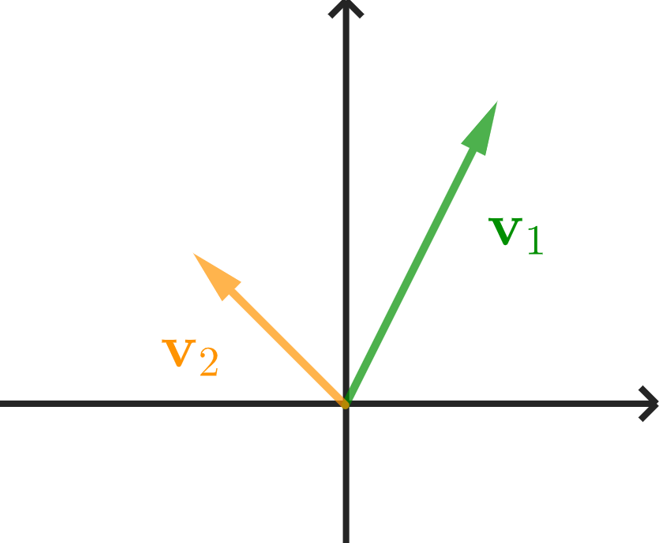
\includegraphics[width=0.6\textwidth, keepaspectratio]{chapters/chapter 4/v1v2 basis.png}
\end{marginfigure}
\[
\vv_1 = \begin{bmatrix} 1 \\ 2 \end{bmatrix}, \qquad \vv_2 = \begin{bmatrix} -1 \\ 1 \end{bmatrix}
\]
վեկտորները նույնպես $\mathbb{R}^2$-ի համար կազմում են հենք, քանի որ դրանք գծորեն անկախ են (ընկած չեն նույն ուղղի վրա), և դրանց թաղանթը $\R^2$-ն է։
\end{example}
  
\begin{example}
\begin{marginfigure}
\centering
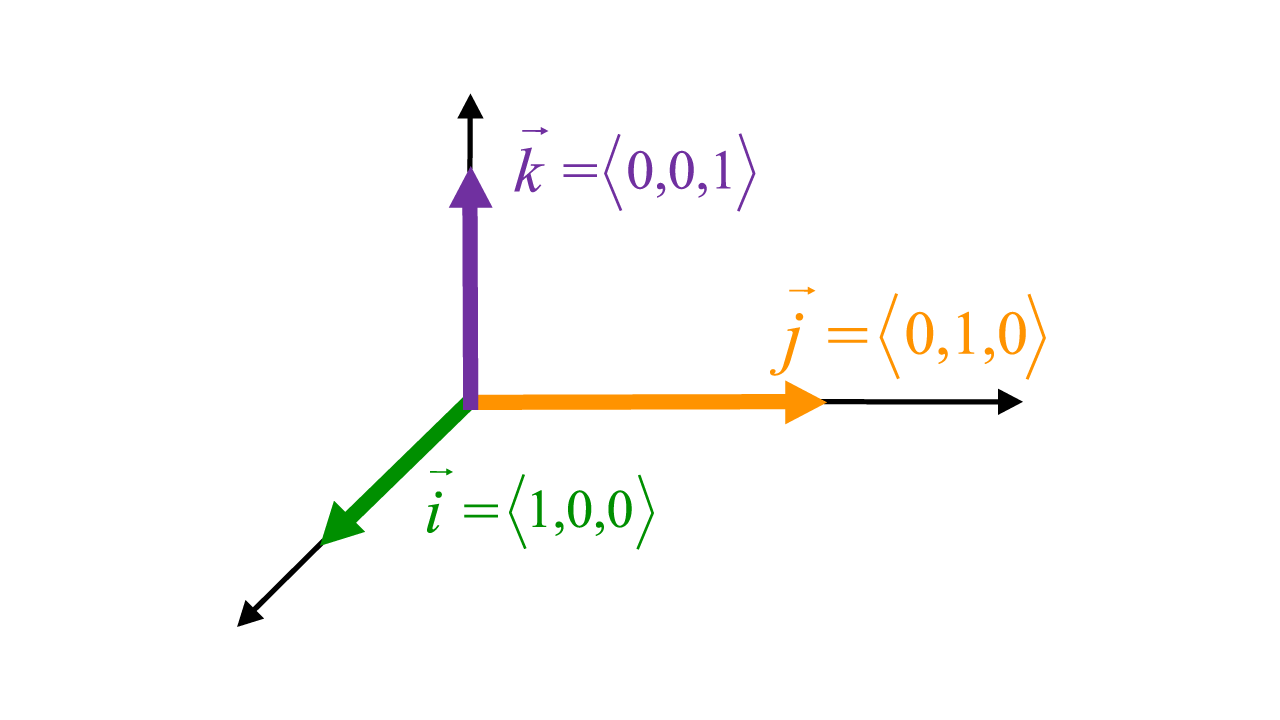
\includegraphics[width=\textwidth, keepaspectratio]{chapters/chapter 4/ijk basis.png}
\end{marginfigure}
\[
\mathbf{e}_1 = \begin{bmatrix} 1 \\ 0 \\ 0 \end{bmatrix}, \qquad \mathbf{e}_2 = \begin{bmatrix} 0 \\ 1 \\ 0 \end{bmatrix}, \qquad \mathbf{e}_3 = \begin{bmatrix} 0 \\ 0 \\ 1 \end{bmatrix}
\]
վեկտորները $\R^3$-ի համար կազմում են հենք ($\R^3$-ի \textit{ստանդարտ հենք}), նշանակվում են նաև՝ $\hat{i}$, $\hat{j}$, $\hat{k}$։
\end{example}

\question{Քանի՞ հենք ունի $\R^2$ տարածությունը։ Իսկ $\R^3$-ը՞։}


\begin{example}
\marginnote[*+2]{չափից դուրս շատ}\[
\vv_1 = \begin{bmatrix} 0 \\ 1 \end{bmatrix}, \qquad 
\vv_2 = \begin{bmatrix} 1 \\ 1 \end{bmatrix}, \qquad 
\vv_3 = \begin{bmatrix} 1 \\ 0 \end{bmatrix}
\]
վեկտորները $\R^2$-ի հենք չեն, քանի որ դրանք գծորեն կախված են։

\marginnote[*+2]{չափից դուրս քիչ}\[
\vv_1 = \begin{bmatrix} 1 \\ 0 \\ 0 \end{bmatrix}, \qquad 
\vv_2 = \begin{bmatrix} 0 \\ 1 \\ 0 \end{bmatrix} 
\]
վեկտորները $\R^3$-ի հենք չեն, քանի որ դրանց թաղանթն ամբողջ $\R^3$-ը չէ (այլ ինչ-որ մի հարթություն)։

\marginnote[*+2]{չափից դուրս անկապ}\[
\vv_1 = \begin{bmatrix} 1 \\ 0 \end{bmatrix}, \qquad 
\vv_2 = \begin{bmatrix} 4 \\ 0 \end{bmatrix} 
\]
վեկտորները $\R^2$-ի հենք չեն, քանի որ դրանք ոչ գծորեն անկախ են, ոչ էլ դրանց թաղանթն է $\R^2$-ը։
\end{example}

\begin{marginfigure}
    \centering
    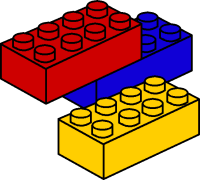
\includegraphics[width=0.6\linewidth]{chapters/chapter 4/lego.png}
    \caption*{հենքի վեկտորները մեր լեգոներն են, որոն\-ցով կառուցում ենք տարածությունը}
\end{marginfigure}

Ինչպես նկատում ենք, ամեն գծային տարածություն ունի բազմաթիվ տարբեր հենքեր (այլ ոչ թե միայն մեկը), բայց այդ բոլոր հենքերը բաղկացած են \textit{միևնույն թվով վեկտորներից։} Այդ թիվը կոչվում է տարածության \textit{չափողականություն։}


\begin{definition}
$V$ գծային տարածության հենքերից յուրաքան\-չյու\-րում եղած վեկտորների թիվը կանվանենք $V$-ի \textbf{չափողա\-կա\-նու\-թյուն} և կնշանակենք $\dim V$-ով։
\end{definition}

Եթե օրինակ $\R^2$-ում վերցնեք նույն ուղղի վրա չընկած երկու վեկտոր (կամ $\R^3$-ում նույն հարթության մեջ չընկած երեք վեկտոր), ապա ինչ վեկտորներ էլ վերցնեք, դրանք կկազմեն հենք։ Ավելի ընդհանուր՝ $\R^n$-ում ցանկացած $n$ հատ գծորեն անկախ վեկտոր կազմում են $\R^n$-ի հենք, հետևաբար՝
\begin{itemize}
    \item $\R^1$-ի չափողականությունը $1$ է
    \item $\R^2$-ի չափողականությունը $2$ է
    \item $\R^3$-ի չափողականությունը $3$ է
    \item $\dots$
    \item $\R^n$-ի չափողականությունը $n$ է
    \item ցանկացած ուղղի չափողականություն $1$ է
    \item ցանկացած հարթության չափողականություն $2$ է
    \item և այլն
\end{itemize}

Երկրաչափորեն չափողականությունը ցույց է տալիս, թե որքան մեծ է տարածությունը, թե ամենաշատը քանի գծորեն անկախ վեկտորներ է կարելի վերցնել այդ տարածության մեջ։

\question{Կարո՞ղ եք գտնել մատրիցներ, որոնք $2\times 2$ չափանի մատ\-րից\-ների տարածության մեջ կազմում են հենք։ Որքա՞ն է $\dim \R^{2 \times 2}$-ը։}


\section{Հենքի փոփոխություն}

Վերադառնանք գծային ձևափոխություններին։ Ընդհանուր առմամբ՝ յուրաքանչյուր մատրից տարածությունը որոշ չափով ձգում, սեղմում ու պտտում է տարբեր ուղղություններով։ Բայց ինչպե՞ս մատրիցի տեսքից հասկանալ, թե այն կոնկրետ ինչ կերպով է ձևափոխում վեկտորները։ Հարցի պատասխանը գտնելու համար դիմենք տարածության հենքի գաղափարին։

\label{matrix_A} Ենթադրենք ունենք հետևյալ ձևափոխությունը՝
\[A = \begin{bmatrix}
    2&1\\1&2
\end{bmatrix}\]


\begin{figure}[h]
    \centering
    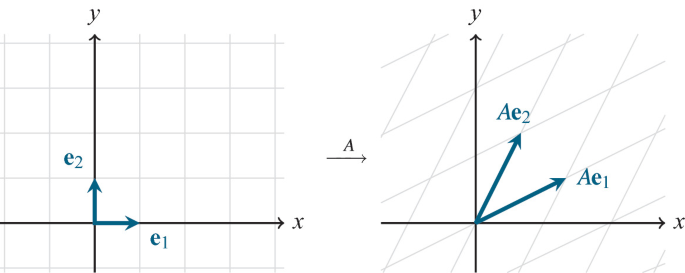
\includegraphics[width=0.75\linewidth]{chapters/chapter 4/viz Av.png}
\end{figure}


Տեսնենք, թե այն ո՞ւր է տանում ստանդարտ հենքի $\ve_1=\begin{bmatrix}
    1 \\ 0
\end{bmatrix}$, $\ve_2=\begin{bmatrix}
    0 \\ 1
\end{bmatrix}$ վեկտորները։

\[
A\ve_1 = \begin{bmatrix}
    2&1\\1&2
\end{bmatrix}\begin{bmatrix}
    1 \\ 0
\end{bmatrix}
=\begin{bmatrix}
    2 \\ 1
\end{bmatrix}
\]
\[
A\ve_2 = \begin{bmatrix}
    2&1\\1&2
\end{bmatrix}\begin{bmatrix}
    0 \\ 1
\end{bmatrix}
=\begin{bmatrix}
    1 \\ 2
\end{bmatrix}
\]

Նկատեցի՞ք․ մատրիցը հենքի $\ve_1$, $\ve_2$ վեկտորները ձևափոխելով տարավ դեպի \textit{իր իսկ սյուները՝}
\[
\begin{bmatrix}
    1 \\ 0
\end{bmatrix} \; \mapsto \; A\text{-ի } 1\text{-ին սյունը}
\]
\[
\begin{bmatrix}
    0 \\ 1
\end{bmatrix} \; \mapsto \; A\text{-ի } 2\text{-րդ սյունը}
\]

Հետևաբար եթե վերցնենք որևէ կամայական $\begin{bmatrix}
    a\\b
\end{bmatrix}$ վեկտոր՝
\begin{align*}
&\begin{bmatrix}a \\ b\end{bmatrix} = a\cdot 
\begin{bmatrix}1 \\ 0\end{bmatrix} + 
b\cdot \begin{bmatrix}0 \\ 1\end{bmatrix} \\
& \qquad \downarrow \qquad \downarrow \qquad  \downarrow \qquad \\
A&\begin{bmatrix}a \\ b\end{bmatrix} = a\cdot 
\begin{bmatrix}2 \\ 1\end{bmatrix} + 
b\cdot \begin{bmatrix}1 \\ 2\end{bmatrix} 
\end{align*}
այն կգնա դեպի նույն գործակիցներով, բայց արդեն $\ve_1$, $\ve_2$-ի փոխարեն՝ $A$-ի առաջին ու երկրորդ սյուներով վեկտորին։ 

Ավելի պատկերավոր ասած՝ բոլոր վեկտորները կառուցված են հենքի վեկտորներից․ 
\begin{itemize}
    \item երկու անգամ ձգենք $\ve_1$-ը՝ ամեն վեկտոր հորիզոնական ուղղու\-թյամբ երկու անգամ կձգվի
    \item վեց անգամ սեղմենք $\ve_2$-ը՝ ամեն վեկտոր ուղղաձիգ ուղղությամբ կսեղմվի
    \item շեղենք $\ve_2$-ը փոքր-ինչ աջ՝ բոլոր վեկտորները համապատասխան չափով կշեղվեն դեպի աջ
\end{itemize}
և այդպես շարունակ։ Ամեն ինչ կարծես կապված է հենքի վեկտորներին․ մատրիցը հենքի վեկտորները պտտելով-ձգելով տանում է իր սյուներին, արդյունքում՝ մյուս բոլոր վեկտորները նույն ձևով պտտվում-ձգվում են։

\question{$A$ մատրիցը $\ve_1$-ը սեղմում է $2$ անգամ, իսկ $\ve_2$-ը տանում է $[0 \quad -3]$ վեկտորին։ Ի՞նչ է լինում $[10 \quad 15]$ վեկտորի հետ։}

Մատրիցների վերաբերյալ խնդիրներ լուծելիս (կամ երբ ուզում եք պարզել, թե ուր է գնում այս կամ այն վեկտորը)\marginnote[*+1]{$2$-չափ կամ $3$-չափ դեպքերում} օգտակար է նայել մատրիցի սյուներին, մտքում պատկերել, թե ինչպես են $\ve_1$ և $\ve_2$ վեկտորները շարժվում դեպի մատրիցի $1$-ին ու $2$-րդ սյուները, և այդպիսով մոտավոր (ոչ շատ ճշգրիտ) պատկերացում կազմել, թե ուր է գնում Ձեր ուզած վեկտորը։

Ամփոփելով՝ արձանագրենք, որ եթե $n\times n$ չափանի $A$ մատրիցի սյուները/տողերը գծորեն անկախ են\marginnote{ասել է թե՝ $A$-ի սյուները $\R^n$-ի հենք են}, ապա այն կիրառելիս կարծես հին՝ $\ve_1$, $\dots$, $\ve_n$ հենքը փոխարինվում է նոր հենքով՝ մատրիցի սյուներով։


\begin{definition}
\marginnote{գծորեն անկախ սյուների և տողերի թիվը համընկնում է}$A$ մատրիցի գծորեն անկախ սյուների/տողերի թիվը կոչվում է $A$ մատրիցի \textbf{ռանգ։}
\end{definition}


\section{Սեփական արժեք և վեկտոր}

Երբեմն դժվար է առանց հաշվարկների ու գործիքների պատկերացնել, թե ինչպես է տրված գծային ձևափոխությունը փոխում այս կամ այն վեկտորը, հատկապես եթե ձևափոխությունը և՛ պտտում, և՛ սեղմում, և՛ ձգում է տարածությունը տարբեր ուղղություններով։ 

Օրինակ՝ \hyperref[matrix_A]{\color{OliveGreen} նախորդ բաժնից} 
\[
A = \begin{bmatrix}
    2 & 1 \\ 1 & 2
\end{bmatrix}
\]
գծային ձևափոխությունը հենքի վեկտորները մի փոքր ձգում է և պտտում՝ $\ve_1$-ը ժամսլաքի ուղղությամբ, $\ve_2$-ը՝ ժամսլաքին հակառակ։ Արդյունքում $x$-երի և $y$-երի առանցքները \marginnote{պատկերացրեք՝ ասես $x$-երի ու $y$-ների առանցքները մկրատի պոչեր են} որոշ չափով ձգվում են և մոտենում իրար․ դրանց կազմած անկյունը փոքրանում է։ 

Արդյունքում ո՞ւր է գնում, ասենք, $\begin{bmatrix}
    -3 \\ 4
\end{bmatrix}$ վեկտորը՝
\[
A\begin{bmatrix}
    -3 \\ 4
\end{bmatrix} = \begin{bmatrix}
    2 & 1 \\ 1 & 2
\end{bmatrix}\begin{bmatrix}
    -3 \\ 4
\end{bmatrix} = \begin{bmatrix}
    -2 \\ 5
\end{bmatrix}
\]

$A$-ն այն և պտտում է, և ձգում տարբեր ուղղություններով, արդյունքում՝ դժվար է առանց հաշվելու միանգամից կռահել, թե $A$-ն կիրառելիս որտեղ է այն գնում։ 

\begin{figure}[h]
    \centering
    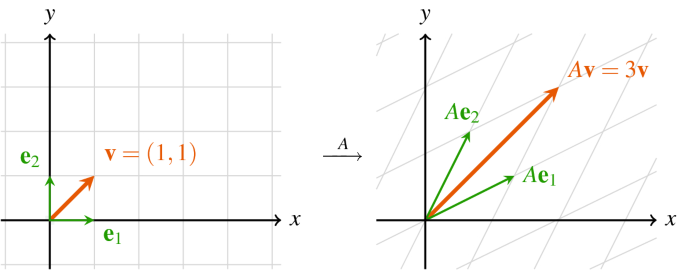
\includegraphics[width=0.75\linewidth]{chapters/chapter 4/viz eig.png}
    \caption*{$\vv$-ն մկրատի «կիսորդն» է}
\end{figure}

Մինչդեռ փոխարենը, եթե $A$-ն ընդամենը որևէ ֆիքսված չափով ձգեր կամ սեղմեր վեկտորը (ասենք՝ $3$ անգամ ձգեր), դա պատկերացնելը շատ ավելի հեշտ կլիներ։ Վերցնենք օրինակ $\vv = \begin{bmatrix}
        1 \\ 1
    \end{bmatrix}$ վեկտորը՝

\[
A \vv = \begin{bmatrix}
    2 & 1 \\ 1 & 2
\end{bmatrix}\begin{bmatrix}
    1 \\ 1
\end{bmatrix} = \begin{bmatrix}
    3 \\ 3
\end{bmatrix} = 3\cdot \begin{bmatrix}
    1 \\ 1
\end{bmatrix} = 3\vv
\]

Օ՜, հրաշք․ ստացանք նույն $\vv$ վեկտորը՝ $3$ անգամ ձգած, ու ոչ մի պտույտ կամ շրջում։

\question{Ինչպե՞ս կփոխվի $\vv$-ի կրկնապատիկը։ Իսկ $-5\vv$՞-ն։}

Առաջին վեկտորի դեպքում դժվար էր պատկերացնել, թե այն ուր է գնում, իսկ այ $\vv$-ի դեպքում ամեն բան ավելի հեշտ է, քանի որ ձևափոխության արդյունքում այն չի պտտվում, այլ մնալով նույն ուղղի վրա՝ պարզապես մի քանի անգամ ձգվում է կամ սեղմվում։ 

Այդպիսի վեկտորների հետ աշխատելը, իհարկե, շատ ավելի հեշտ է ու նախընտրելի։ Դրանք ունեն հատուկ անուն և կոչվում են գծային ձևափոխության/մատրիցի \textit{սեփական} \marginnote{$3$-ը $A$-ի սեփական արժեք է}վեկտորներ, իսկ դրանց ձգման/\linebreak սեղմման գործակիցները՝ \textit{սեփական} արժեքներ։

\begin{definition}
Եթե որևէ $\lambda$ թվի և $\vv$ ոչ զրոյական վեկտորի համար
\[
A\vv=\lambda\vv
\]
ապա կասենք, որ \marginnote{անգլերեն՝ {\it eigenvalue} և {\it eigenvector}}
\begin{itemize}
    \item $\lambda$-ն $A$-ի \textbf{սեփական արժեք} է
    \item $\vv$-ն $\lambda$-ին համապատասխան \textbf{սեփական վեկտոր} է
\end{itemize}
\end{definition}


\begin{example}
\[
A = \begin{bmatrix}
 3 & 5 \\ 1 & -1   
\end{bmatrix}
\]
գծային ձևափոխությունը  $\vv = \begin{bmatrix}
5 \\ 1
\end{bmatrix}$ վեկտորը ձգում է $4$ անգամ՝
\[A\vv =  
\begin{bmatrix}
3 & 5 \\ 1 & -1 
\end{bmatrix}
\begin{bmatrix}
5 \\ 1
\end{bmatrix}
=
\begin{bmatrix}
20 \\ 4
\end{bmatrix}
=4\vv
\]
հետևաբար $\lambda = 4$-ը $A$-ի սեփական արժեք է, իսկ $\vv$-ն՝ սեփական վեկտոր։ 
\end{example}

Եթե $A\vv=\lambda \vv$, ապա $\vv$-ի փոխարեն տեղադրելով $3\vv$, $-3\vv$, և այլն՝ ստանում ենք, որ $\vv$-ի հետ նույն ուղղի վրա ընկած ցանկացած վեկտոր նույնպես $A$-ի սեփական վեկտոր է ($\lambda$ սեփական արժեքին համապատասխան)։ 
\begin{theorem}
Եթե $\vv$-ն $A$-ի սեփական վեկտոր է, ապա $c\vv$-ն ևս $A$-ի սեփական վեկտոր\marginnote{նույն արժեքին համապատասխան} է (ցանկացած $c\ne 0$ թվի համար)։
\end{theorem}

Ուրեմն եթե $\lambda$ թիվը $A$-ի սեփական արժեք է, ապա $A$-ն ոչ թե ունի մեկ-երկու վեկտոր, այլ ամբողջական \textit{ուղղություններ,} որոնց վրա կիրառելիս դրանք պարզապես $\lambda$ անգամ ձգում է։ 

\question{Կարո՞ղ է $\vv$ վեկտորը համապատասխանել երկու տարբեր $\lambda_1$ և $\lambda_2$ սեփական արժեքների։}

$A$-ի բոլոր սեփական արժեքների բազմությունը անվանում են $A$-ի \textit{սպեկտր,} իսկ յուրաքանչյուր $\lambda$ սեփական արժեքին համապատասխանող սեփական վեկտորների բազմությունը՝ $\lambda$-ին համապատասխան \textit{սեփա\-կան տարածություն}\marginnote{անգլերեն՝ {\it eigenspace}} (նշանակում են՝ $E_\lambda$):

\warning{$n\times n$ չափանի մատրիցը ամենաշատը կարող է ունենալ $n$ սեփական արժեքներ, կարող է նաև ընդհանրապես չունենալ։}

\question{Կարո՞ղ եք նկարագրել $\R^2$-ի այնպիսի ձևափոխություն, որը սեփական արժեք չունի։ Իսկ այնպիսին, որն ունի ուղիղ մեկը՞։}

Ինչպե՞ս մատրիցի հետ թվաբանական գործողություններ անելով գտնենք նրա սեփական արժեքները։ Եկեք պարզենք դա՝ առանց հաշվողական մասի վրա խորանալու։ Ուզում ենք գտնել այնպիսի $\lambda$ և $\vv$, որ $A\vv= \lambda \vv$։ Նշանակենք $\lambda$-ն $x$-ով և գրենք՝
\[
A\vv= x \vv = x(I\vv) = (xI)\vv
\]
կամ որ նույնն\marginnote{ի՞նչ տեսք ունի $xI$ մատրիցը} է՝ $A\vv-(xI)\vv = (A-xI)\vv= \mathbf{0}$:

Եթե $(A-xI)$ մատրիցը ունենար հակադարձ, կգրեինք՝
\[
\vv = (A-xI)^{-1}\mathbf{0}
\]
բայց ցանկացած մատրիցի և $\mathbf{0}$-ի արտադրյալը հենց $\mathbf{0}$ է, ուրեմն կստացվեր $\vv = \mathbf{0}$, բայց չէ՞ որ պահանջել էինք, որ սեփական վեկտորը զրոյական չլինի։ Հետևաբար $(A-xI)$-ն հակադարձ չունի՝
\[
\det(A-xI)=0
\]

Ահա այս հավասարման ձախ մասում գրվածը որոշիչի բանաձևով կբացենք, կստանանք $x$-ից կախված մի բազմանդամ (կոչվում է՝ $A$-ի \textit{բնութագրիչ բազմանդամ}), և եթե գտնենք դրա արմատները՝ ստացված թվերը կլինեն $A$-ի սեփական արժեքները։ Խնդրի լուծման կոնկրետ օրինակ կարող եք տեսնել օրինակ՝ \href{https://www.youtu.be/UVZ4kStUo1s}{այստեղ}, սակայն ինչպես մեծ չափանի մատրիցների որոշիչի, այնպես էլ սեփական արժեքների դեպքում՝ ձեռքով դրանց հաշվելը երկար գործ է, ուստի մենք դրա վրա չենք կենտրոնանա։

Փոխարենը, հետևյալ գեղեցիկ հատկությունները կապ են հաստատում գծային ձևափոխության երեք տարբեր բնութագրիչների՝ սեփական արժեքների, որոշիչի և հետքի միջև․
\begin{theorem}
Քառակուսային մատրիցի որոշիչը հավասար է նրա սեփական արժեքների արտադրյալին․
\[
\det(A) = \lambda_1 \cdot \lambda_2 \cdot \ldots \cdot \lambda_n
\]
իսկ \marginnote{սիրուն է, չէ՞} հետքը՝ սեփական արժեքների գումարին․
\[
\operatorname{tr}(A) = \lambda_1 + \lambda_2 + \ldots + \lambda_n
\]
\end{theorem}



\bigskip 

\begin{theory}
.
\begin{itemize}
\item կարդալ [{\rm Johnston}], 126-129 (գծային թաղանթ), 131-135 (գծորեն անկախություն), 140-141 (հենք) էջերը  
\item դիտել  {\rm 3b1b}-ի \href{https://www.3blue1brown.com/lessons/span}{2-րդ} տեսադասը գծային հանրահաշվից 
\item կարդալ [{\rm Poole}], 202-203 էջերը (չափողականություն)
\item վերադառնալ [{\rm Johnston}], 38-41 և 235-237 (մատրիցի սյունե\-րի և հենքի կապը), 285-286 (սեփական արժեքներ) էջերին
\item ըստ ցանկության՝ [{\rm Poole}], 255-259 էջերի օրինակներին
\item դիտել {\rm 3b1b}-ի \href{https://www.3blue1brown.com/lessons/eigenvalues}{14-րդ} տեսադասը գծային հանրահաշվից 
\item տեսնել սեփական վեկտորները \href{https://setosa.io/ev/eigenvectors-and-eigenvalues}{սեփական աչքով}
\item ըստ ցանկության՝ հետազոտել \href{https://www.youtu.be/mhy-ZKSARxI}{սեփական արժեքներով} և \href{https://www.ams.org/publicoutreach/feature-column/fcarc-svd}{եզակի արժեքներով} մատրիցի վերլուծության մասին
\end{itemize}
\end{theory}

\newpage

\section{Խնդիրներ}


\begin{problem}\marginnote[*+0.5]{\href{https://youtu.be/5VEnDdm8RZo}{լուծում}}
Լրացրեք բացակայող թվերը՝
\[
\begin{bmatrix}
    2 & * \\ -1 & *
\end{bmatrix}
\]
եթե հայտնի է, որ
\begin{enumerate}[label={\alph*}․]
\item ձևափոխությունը ձգում է $\begin{bmatrix}
    1 & 0
\end{bmatrix}$ վեկտորը $2$ անգամ

\item ձևափոխությունը հետքը $2$ է, իսկ որոշիչը՝ $3$

\item $1$-ն ու $5$-ը ձևափոխության սեփական արժեքներ են
\end{enumerate}

\end{problem}

\begin{problem}
Ամենաշատը ի՞նչ չափողականության ենթատարածություն է կարելի կառուցել այս վեկտորներով․
\begin{enumerate}[label={\alph*}․]
\item $\vv_1=\begin{bmatrix}6\\1\\5\end{bmatrix}$,  $\vv_2=\begin{bmatrix}
    2\\3\\2
\end{bmatrix}$

\item $\vv_1=\begin{bmatrix}6\\2\end{bmatrix}$,  $\vv_2=\begin{bmatrix}
    1\\3
\end{bmatrix}$,  $\vv_3=\begin{bmatrix}
    5\\2
\end{bmatrix}$

\item $\vv_1=\begin{bmatrix}4\\1\\2\end{bmatrix}$,  $\vv_2=\begin{bmatrix}
    -4\\2\\-1
\end{bmatrix}$,  $\vv_3=\begin{bmatrix}
    8\\-1\\7
\end{bmatrix}$

\item $\vv_1=\begin{bmatrix}3\\-2\\1\end{bmatrix}$, $ \vv_2=\begin{bmatrix}
    6\\-4\\4
\end{bmatrix}$
\end{enumerate}
\end{problem}


\begin{problem}
Գտեք հետևյալ ձևափոխությունների սեփական արժեքներն ու վեկտորները․

\begin{enumerate}[label={\alph*}․]
\item $A=\begin{bmatrix}
    1&2\\0&1\end{bmatrix}$

\item $B=\begin{bmatrix}
    2&1\\1&2
\end{bmatrix}$

\item $C=\begin{bmatrix}
    8 & 1 \\ 8 & 1
\end{bmatrix}$

\item $D=\begin{bmatrix}
-1&0&0\\0&1&0\\0&0&3        \end{bmatrix}$
\end{enumerate}

Կարող եք օգտվել մեր իմացած ցանկացած մեթոդից (բնութագրիչ բազմանդամ, հետք և որոշիչ, սյուների ու հենքի կապը), բայց փորձեք նաև տեսողաբար պատկերացնել խնդիրը։
\end{problem}



\begin{problem}
Ենթադրենք ունենք
\[
A=\begin{bmatrix}
    a_1 & 0 & 0 & 0 & 0 \\
    0 & a_2 & 0 & 0 & 0 \\
    0 & 0 & a_3 & 0 & 0 \\
    0 & 0 & 0 & a_4 & 0 \\
    0 & 0 & 0 & 0 & a_5 
\end{bmatrix}
\]
գծային ձևափոխությունը, որտեղ $a_1, \dots, a_5$-ը որևէ ֆիքսված դրական թվեր են։
\begin{enumerate}[label={\alph*}․]
\item ո՞րն է $\mathbb{R}^5$ տարածության ստանդարտ հենքը

\item ո՞ւր է տանում $A$-ն $\mathbb{R}^5$-ի ստանդարտ հենքի վեկտորներին

\item ի՞նչ եք կարծում, որքա՞ն է $A$-ի որոշիչը

\item կարո՞ղ եք գտնել $A$-ի սեփական արժեքներն ու վեկտորները
\end{enumerate}


\end{problem}


\begin{problem}
Ֆեյսբուքում հանդիպելով հետևյալ խնդրին՝
\begin{quote}
\textit{$2$ խնձորն ու $3$ տանձը միասին արժեն $1100$ դրամ, իսկ $1$ խնձորն ու $4$ տանձը՝ $700$ դրամ։ Միայն $140$-ից բարձր {\it IQ} ունեցող մարդիկ կարող են գտնել խնձորի ու տանձի գինը։}
\end{quote}
հասկանում եք, որ եկել է պահը՝ վերջապես կիրառելու Ձեր սովորածը։
\begin{enumerate}[label={\alph*}․]
\item անհայտները նշանակելով $x_1$, $x_2$-ով՝ գրեք խնդիրը համակարգի տեսքով

\item կարո՞ղ եք պայմանները արտահայտել
\[
\begin{bmatrix}
    * & * \\ * & *
\end{bmatrix}\begin{bmatrix}
    x_1 \\ x_2
\end{bmatrix}
= \begin{bmatrix}
    * \\ *
\end{bmatrix}
\]
տեսքով, կարճ՝ $A\vx = \vb$

\item օգտվելով հակադարձի բանաձևից՝ փորձեք գտնել $\vx$-ը
\end{enumerate}

Այն, ինչ ստացաք, կոչվում է \textit{գծային հավասարումների համակարգ։}

\end{problem}

\setchapterpreamble[u]{\margintoc}
\chapter{Մեկ փոփոխականի ֆունկցիա}
\labch{single_var}

\emergencystretch 2em

\section{Էքստրեմումի խնդիր}\label{apricot}

Պատկերացրեք՝ վեկտորների փոխարեն ունեք խանութ, և որոշակի հաշվարկների արդյունքում ստացել եք, որ խանութի եկամուտը ծիրանի գնից կախված է հետևյալ բանաձևով՝
\[
f(x) = 20\sqrt{x}-3x^3
\]
որտեղ $x$-ը $1$ կգ ծիրանի գինն է։

Ինչպես ցանկացած գործարար, Դուք ուզում եք հնարավորինս մեծացնել Ձեր եկամուտը, ուստի Ձեզ հետաքրքրում է հետևյալ հարցը․

\textit{— Որքա՞ն պետք է լինի $x$-ը, որպեսզի $f(x)$-ը լինի մաքսիմալ՝ հնարավորինս մեծ}

\question{\href{https://www.desmos.com}{\it Desmos} կամ \href{https://www.geogebra.org}{\it GeoGebra} ծրագրով գծեք $f(x)$-ի գրաֆիկը։ Ո՞րն է ծիրանի օպտիմալ գինը։}

Իրական կյանքում, իհարկե, իրավիճակն ավելի բարդ է, քանի որ ամեն խանութ ծիրանից բացի ուրիշ ապրանքներ էլ է վաճառում։ Եկամուտը կարող է կախված լինել մի քանի տարբեր գործոններից, օրինակ՝
\[
f(x,y,z,t) = 3xy^2-y\log t - (1-y) \log(1-t) + \frac{z^3}{t}
\]
որտեղ $x$, $y$, $z$, $t$-ի տվյալ պահին ունեցած արժեքներն են 
\[
x=4, \qquad y=0.4, \qquad z=0.8, \qquad t=55
\] 
և անհրաժեշտ է որոշել՝ մեծացնե՞լ, թե՞ փոքրացնել այդ արժեքները (և որքանո՞վ)։

Մեքենայական ուսուցման մեջ հաճախ նման անհայտները \marginnote{հաճախ այս խնդիրը անհնար է լու\-ծել․ փոխարենը որոնում են ոչ թե \textit{ամենա\-մեծ,} այլ \textit{համեմատաբար մեծ} արժեք} (պարա\-մետ\-րերը) ոչ թե մեկն են, այլ միլիոնից ավել, սակայն խնդիրը մնում է նույնը․ ինչպե՞ս գտնել տվյալ մեծության ամենամեծ կամ ամենափոքր արժեքը։ 

Նմանատիպ խնդիրները կոչվում են \textit{էքստրեմումի խնդիրներ,} և մենք կսկսենք մեր քննարկումը այն դեպքից, երբ ունենք միայն մի փոփոխական պարամետր։


\section{Հաջորդականություններ}

Սկսենք հաջորդականություններից։ \textit{Հաջորդականություն} ասելով՝ նկա\-տի կունենանք \textbf{անվերջ քանակով} թվերի՝ ֆիքսված հերթականու\-թյամբ գրված «շարք», «շարան»։

\begin{example}
Սրանք հաջորդականություններ են՝
\begin{itemize}
    \item $1,\; 2,\; 3,\; 4,\; 5,\; \dots$
    \item $1,\; -1,\; 1,\; -1,\; 1,\; \dots$
    \item $0,\; 0.2,\; 0.4,\; 0.6,\; 0.8,\; \dots$
    \item $6,\; 6,\; 6,\; 6,\; 6,\;  \dots$
\end{itemize}
իսկ սա՝ ոչ․
\begin{itemize}
    \item $1,\; 2,\; 3,\; 4$
\end{itemize}
\end{example}


Ինչ-որ իմաստով՝ հաջորդականությունը մեր իմացած վեկտորն է, բայց անվերջ երկարությամբ։ Ինչպես վեկտորները նշանակում ենք տառով՝
\[
\vv = \begin{bmatrix}
    v_1 \\ v_2 \\ \vdots \\ v_n
\end{bmatrix}
\]
իսկ նրա բաղադրիչները՝ նույն տառ + համարակալումով, այնպես էլ ամեն հաջորդականության կարող ենք տալ ինչ-որ անուն, ասենք՝ $a$, իսկ դրա \textit{անդամները} համարակալել՝
\[
a = (a_1,\, a_2,\, a_3,\, a_4,\, \dots )
\]

Քանի որ հաջորդականության բոլոր անդամները հերթով թվարկելն անհնար է (անվերջ հատ են), սովորաբար հարմարության համար պարզապես կգրենք, թե ի՞նչ բանաձևով է որոշվում դրա $n$-րդ ընդհանուր անդամը՝ $a_n$-ը։ 

Օրինակ՝ եթե ուզում ենք խոսել բնական թվերի քառակուսիներից բաղկացած հաջորդականության ($=$անվերջ չափանի վեկտորի) մասին, կգրենք՝
\[
a_n = n^2 \qquad \text{կամ} \qquad \{a_n\}=\{n^2\}
\]
և նկատի կունենանք, որ
\[
a_1 = 1, \qquad a_2 = 4, \qquad a_3 = 9, \qquad \dots 
\]
այսինքն՝ $a = (1,\, 4,\, 9,\, \dots)$:

\warning{Բազմություններում տարրերի հերթականությունը կարևոր չէ, մինչդեռ հաջորդականությունների դեպքում շատ կարևոր է․ $(1,\, 2,\, 3,\, 4,\, \dots) \ne (2,\, 1,\, 3,\, 4,\, \dots)$:}

Վեկտորների նմանությամբ կսահմանենք նաև հաջորդականությունների գումարը, տարբերությունը և թվով բազմապատկումը՝
\begin{align*}
(a_1,\, a_2,\, a_3,\, \dots) 
\pm
(b_1,\, b_2,\, b_3,\, \dots) 
&=
(a_1\pm b_1,\, a_2\pm b_2,\, a_3\pm b_3,\, \dots)% = a\pm b
\\
c \cdot 
(a_1,\, a_2,\, a_3,\, \dots) 
&=
(ca_1,\, ca_2,\, ca_3,\, \dots)% =c\cdot a
\end{align*}

Եթե բոլոր հաջորդականությունների բազմությունը նշանակենք $c$-ով, ապա $c$-ն կլինի գծային տարածություն (ինչպես վեկտորների բազմու\-թյունները)։ Ի տարբերություն վեկտորների՝ կսահմանենք նաև հաջոր\-դա\-կանությունների անդամ առ անդամ բազմապատկում և բաժանում՝
\begin{align*}
ab &= (a_1b_1,\, a_2b_2,\, a_3b_3,\, \dots) \\
\frac{a}{b}&=
\left(\frac{a_1}{b_1},\, \frac{a_2}{b_2},\, \frac{a_3}{b_3},\, \dots\right) \qquad \text{եթե $b_1, b_2, \dots \ne 0$}
\end{align*}

\question{Ի՞նչ հաջորդականությամբ բազմապատկենք $(1,\, 2,\, 3,\, 4,\, \dots)$ հաջորդականությունը, որպեսզի այն դառնա $(0,\, 0,\, 3,\, 0,\, 0,\, \dots)$:}

\section{Հաջորդականության սահման}

Կան հաջորդականությունների շատ հետաքրքիր օրինակներ։ Վերցնենք, օրինակ, հետևյալ հաջորդականությունը՝ $a_n = \dfrac{1}{n}$, այսինքն՝
\[
\left(1,\quad  \frac{1}{2},\quad \frac{1}{3},\quad \frac{1}{4},\quad \frac{1}{5},\quad \dots\right)
\]

Նկատենք, որ որքան $n$-ը մեծանում է, այնքան հաջորդականությունը փոքրանում ու փոքրանում է։ 

\begin{description}
    \item[Կա՞ այնպիսի թիվ, որին $\{a_n\}$-ը գնալով մոտենում է․] այո՛, որքան $n$-ը մեծանում է՝ $n\to\infty$, այնքան $a_n$-ը մոտենում է զրոյի՝ $a_n\to 0$։ Այս դեպքում $0$-ն կանվանենք $\{a_n\}$-ի \textit{սահման։}

    \item[Ինչ-որ պահի $a_n$-ը դառնո՞ւմ է $0$․] ո՛չ, հետաքրքիր է, սակայն որքան էլ հաջորդականության անդամները ձգտում են $0$-ին, մինևույն է՝ չեն հասնում, միշտ մնում են զրոյից մեծ։
\end{description}

\begin{definition}
Կասենք, որ  $\{a_n\}$ հաջորդականությունը \textbf{ձգտում} կամ \textbf{զուգամիտում} է $L$ թվին (կամ՝ $L$-ը $\{a_n\}$-ի \textbf{սահմանն} է), եթե $n$-ի բավարար մեծ արժեքների դեպքում բոլոր $a_n$ անդամները որքան ասես մոտ են լինում $L$-ին։

Դա կգրառենք այսպես՝
\marginnote{անգլերեն՝ {\it limit}, լատիներեն՝ {\it limes}}\[
\lim_{n\to\infty} a_n = L
\]
կամ այսպես՝
\[
a_n \to L \qquad (\text{երբ } n\to\infty)
\]
\end{definition}

Ի՞նչ նկատի ունենք, երբ ասում ենք՝ բնական թվերը անվերջ են։ Նկատի ունենք, որ ինչ թիվ էլ վերցնենք, գոյություն ունի այնպիսի բնական թիվ, որը դրանից ավելի մեծ է։ Նույն ձևով, երբ ասում ենք՝ $a_n \to L$, նկատի ունենք՝ ինչքան փոքր թիվ էլ վերցնենք (ասենք՝ $0.0001$) և հարցնենք՝ արդյո՞ք ինչ-որ պահի հաջորդականության բոլոր անդամները գտնվելու են $L$-ից ամենաշատը $0.0001$ հեռավորության վրա (այսինքն՝ շատ մոտիկ), պատասխանը լինելու է՝ \marginnote{այսինքն՝ կա ինչ-որ $N$ համար (ասենք՝ $N=2000$), որ դրանից հետո եկող բոլոր $n$-երի դեպքում՝ $|a_n-L|<0.0001$} այո, \textit{այսինչ պահից սկսած՝ բոլոր $a_n$-երը լինելու են $L$-ին $0.0001$ չափով մոտ։} 

\phantomsection \label{eps-delta}Ուստի կարող ենք $\lim\limits_{n\to\infty} a_n=L$ երևույթը ձևակերպել նաև այսպես՝
\begin{itemize}
 \item ինչ $\varepsilon>0$ թիվ էլ վերցնես
 \item գոյություն ունի բավարար մեծ $N$ թիվ այնպես, որ 
 \item $|a_n - L|<\varepsilon$ բոլոր $n=N,\ N+1,\ N+2,\ \dots$ անդամների համար
\end{itemize}

Նման ձևով կսահմանենք, որ $\lim\limits_{n\to\infty} a_n=+\infty$, եթե $a_n$-ը ցանկացած թվից մեծ է դառնում որոշ թվով քայլերից հետո։

\begin{definition}
Եթե $\{a_n\}$-ն ունի սահման, և այդ սահմանը վերջավոր է, ապա կասենք, որ այն \textbf{զուգամետ} է, հակառակ դեպքում՝ \textbf{տարամետ} է։
\end{definition}
    

\begin{example}
\\~
\begin{itemize}
    \item $1,\, 2,\, 3,\, 4,\, 5,\, \dots  \to +\infty$ 
    \item $1,\, -1,\, 1,\, -1,\, 1,\, \dots$ սահման չունի
    \item $0,\, 0.2,\, 0.4,\, 0.6,\, 0.8,\, \dots \to +\infty$
    \item $6,\, 6,\, 6,\, 6,\, 6,\,  \dots  \to 6$
\end{itemize}
\end{example}

\warning{Հաջորդականությունը կարող է ինչ-որ պահից սկսած հավասար լինել կամ չլինել իր սահմանին։}

Հաճախ կարելի է հաջորդականության բանաձևից որոշել նրա սահմանը․
\begin{itemize}
    \item $n^k \to \infty$ ցանկացած $k>0$ թվի համար
    \item $\dfrac{1}{n^k} \to 0$ ցանկացած $k>0$ թվի համար
    \item \marginnote{ի՞նչ կլինի, եթե $|c|=1$}$c^n\to +\infty$, եթե $c>1$, բայց $c^n \to 0$, եթե $|c|<1$
    \item եթե ինչ-որ պահից սկսած հաջորդականության բոլոր անդամները հավասար են նույն թվին, սահմանը այդ թիվն է 
\end{itemize}

\question{Ամեն ուրբաթ Ձեր տնօրենը կանչում է և ուրախությամբ հայտնում, որ Ձեր աշխատավարձը բարձրացվում է $0.99$ անգամ։ Քանի՞ շաբաթից կսկսեք զգալ, որ մի բան այն չէ։}

\begin{example}
\\~
\begin{itemize}
    \item $\lim\limits_{n \to \infty} \dfrac{1}{n} = 0$
    
    \item $\lim\limits_{n \to \infty} \left(\dfrac{2}{3}\right)^n  = 0$

    \item $\lim\limits_{n \to \infty} 0.3n  = \infty$ \; (տարամետ է)
\end{itemize}
\end{example}

Նկատենք նաև, որ երկու զուգամետ հաջորդականություններ գումարելիս, բազմապատկելիս, և այլ գործողություններ անելիս դրանց սահմանները պահպանվում են, այսինքն՝

\newpage
\begin{theorem}\label{limit_properties}
\\~
\begin{enumerate}
\item \marginnote{այստեղ $L$-ն ու $M$-ը \textbf{վերջավոր} թվեր են}Եթե $\lim\limits_{n \to \infty} a_n = L$ և $\lim\limits_{n \to \infty} b_n = M$, ապա
    \begin{align*}
        &\lim\limits_{n \to \infty} (a_n + b_n) = L + M\\
        &\lim\limits_{n \to \infty} (a_n - b_n) = L - M\\
        &\lim\limits_{n \to \infty} (a_n \cdot b_n) = L \cdot M\\
        &\lim\limits_{n \to \infty} \frac{a_n}{b_n} = \frac{L}{M} \qquad  \text{(եթե $M\ne0$)}
    \end{align*}
        
\item Եթե $\lim\limits_{n \to \infty} a_n = L$, ապա ցանկացած $c$ թվի համար
    \[
    \lim\limits_{n \to \infty} (c \cdot a_n) = c \cdot L
    \]
\begin{marginfigure}
    \caption*{$b$-ն սեղմված է $a$-ի ու $c$-ի արանքում, որոնք ձգտում են նույն $L$-ին}
    \centering
    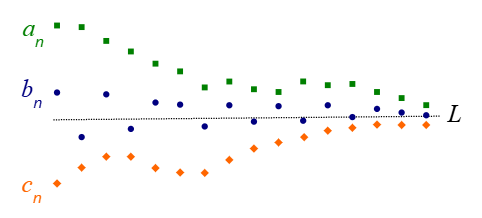
\includegraphics[width=\linewidth]{chapters/chapter 5/squeeze.png}
\end{marginfigure}
\item Եթե ցանկացած $n$-ի համար 
\[
a_n \leq b_n \leq c_n
\]
և $\lim\limits_{n \to \infty} a_n = \lim\limits_{n \to \infty} c_n = L$, ապա $\lim\limits_{n \to \infty} b_n = L$։
\end{enumerate} 
\end{theorem}

\question{Ենթադրենք $a_n \to 4$։ Ո՞ւր կձգտի հաջորդականությունը, եթե հեռացնեք նրա առաջին $3$ անդամները։}

Քանի որ ինչ-որ սահմանի ձգտելու համար անհրաժեշտ է, որ հաջորդա\-կանության անդամները \textit{սկսած ինչ-որ պահից} մոտ լինեն այդ սահմանին, նշանակում է՝ այդ սահմանը կախված չէ հաջորդականության առաջին $3$, $100$ կամ $1000$ անդամներից։ Եթե ի վերջո հաջորդականու\-թյու\-նը մոտենում է ինչ-որ թվի, ապա սկզբի մի քանի անդամներ\marginnote{թեև, իհարկե, ամեն բան կարող է փոխվել, եթե ջնջեք կամ ավելացնեք \textit{անվերջ թվով} անդամներ} փոխելիս, ջնջելիս կամ ավելացնելիս այդ զուգամիտությունը չի փոխ\-վում։

\section{Ֆունկցիայի սահման}

\question{Ի՞նչ եք կարծում, ի՞նչ է նշանակում $\lim\limits_{x\to 0} \left(2+x\right)^3$ արտա\-հայտու\-թյունը։}

Ինչպես հաջորդականությունների համար $n$-ը ձգտեցնելով անվերջի և մոտենալով ինչ-որ թվի՝ այն անվանեցինք սահման, այդպես էլ ներմուծենք սահմանի գաղափարը ֆունկցիաների համար։ 

Վերցնենք օրինակ՝
\[
f(x) = \left(2+x\right)^3
\]
ֆունկցիան։ Ո՞ր մեծությունը կուզեինք անվանել $f(x)$-ի սահման $x=0$ կետում։ Ինտուիտիցիան մեզ հուշում է, որ եթե գծեինք $f(x)$-ի գրաֆիկը և նայեինք, թե $x$-ը $0$-ին մոտենալիս ի՞նչ թվի է մոտենում $f(x)$-ի արժեքը, հենց այդ թիվն էլ պետք է որ համարել \textit{$f$-ի սահմանը $0$ կետում։}

Այլ կերպ ասած՝ եթե $0$-ի ձգտող ինչ $\{x_n\}$ հաջորդականություն էլ վերցնենք ու տեղադրենք $f$-ի մեջ, և արդյունքում ստացվող $\left(f(x_1),\, f(x_2),\, f(x_3),\, \dots\right)$ հաջորդականությունը ձգտի ինչ-որ թվի, սահմանը կլինի այդ թիվը։ Ուրեմն սահմանենք $a \in \R$ կետում $f$-ի սահմանը․

\begin{definition}
Եթե \textbf{ցանկացած} $x_n\to a$ հաջորդականության համար
\[
f(x_1), \;\; f(x_2), \;\; f(x_3), \;\; \dots,\;\;f(x_n),\;\;\dots
\]
հաջորդականությունը ձգտում է միևնույն $L$ թվին, ապա $L$-ը կոչվում է $f$ ֆունկցիայի \textbf{սահման $a$ կետում՝}
\[
\lim\limits_{x\to a} f(x) = L
\]
\end{definition}

\begin{figure}[t]
    \centering
    \subfloat{{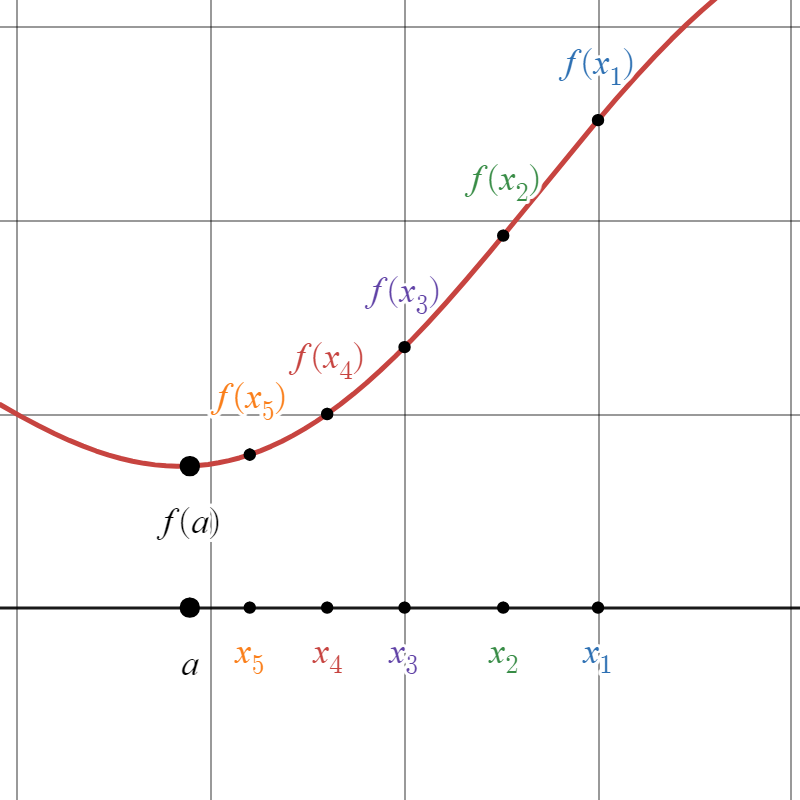
\includegraphics[width=0.4\linewidth]{chapters/chapter 5/cont limit.png} }}%
    \qquad
    \subfloat{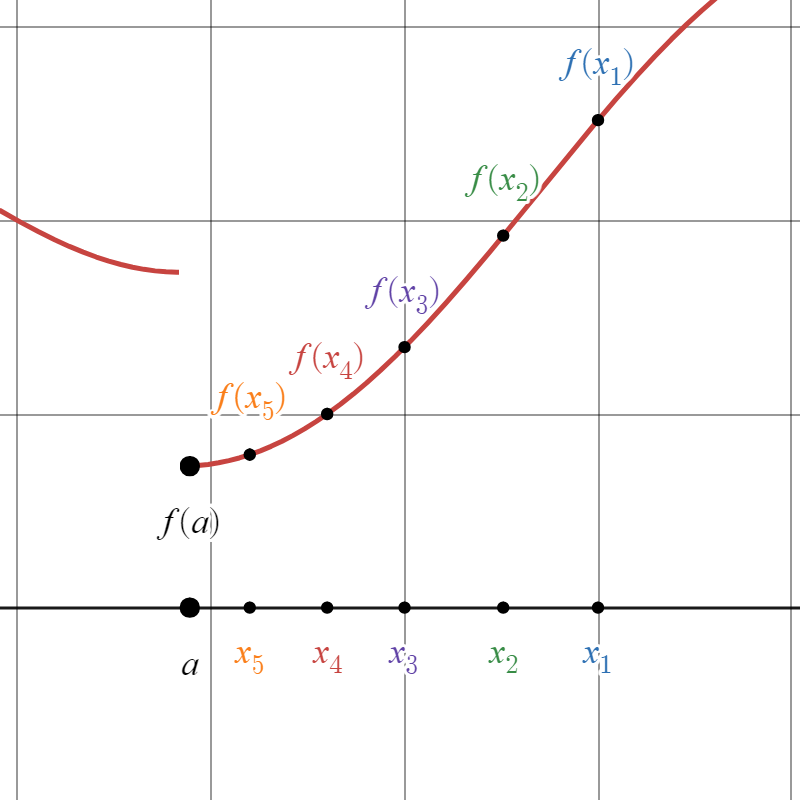
\includegraphics[width=0.4\linewidth]{chapters/chapter 5/disc limit.png}} %
    \caption*{ձախ նկարի ֆունկցիան $a$ կետում ունի սահման, իսկ աջինը՝ չունի, քանի որ եթե $x_n$-երը վերցնեինք $a$-ից ձախ, $f(x_n)$-ը կմոտենար մի ուրիշ թվի}
\end{figure}

Ինչո՞ւ ենք նշում «\textit{ցանկացած} $x_n \to a$-ի համար»։ Բանն այն է, որ երբեմն որոշ ֆունկցիաներ իրենց այնքան էլ լավ չեն պահում․ երբ $a$-ին մոտենում ենք աջից, ստանում ենք ինչ-որ սահման, բայց երբ մոտենում ենք ձախից՝ ստանում ենք մեկ այլ սահման։ Նման դեպքերում կասենք, որ ֆունկցիան $a$ կետում սահման չունի։

\warning{Ֆունկցիան կարող է մի կետում ունենալ սահման, մի ուրիշ կետում՝ ոչ։}

Կրկին ինչպես \hyperref[eps-delta]{\color{OliveGreen}հաջորդականությունների դեպքում}, սահմանը կարող ենք սահմանել նաև այսպես․ կասենք, որ $\lim\limits_{x\to a}f(x)=L$, եթե \marginnote{ինչքան էլ փոքր $\varepsilon$ ասես՝ եթե $x$-ը $a$-ին բավարար մոտ լինի, ապա $f(x)$-ը մոտ կլինի $L$-ին (ոչ հեռու, քան $\varepsilon$ չափով)} ցանկացած $\varepsilon>0$ թվի համար գոյություն ունի այնպիսի $\delta>0$ թիվ, որ եթե $0<|x-a|<\delta$, ապա $|f(x)-L| < \varepsilon$:

\begin{example}
\\~
\begin{itemize}
    \item $\lim\limits_{x \to 0}(2+x)^3 = 2^3 = 8$
    \item $\lim\limits_{x \to 4}(2+x)^3 = 6^3 = 216$
    \item $\lim\limits_{x \to -3}(2+x)^3 = (-1)^3 = -1$
    \item $\lim\limits_{x \to 2.5}4x-3 = 4\cdot 2.5-3 = 7$
    \item $\lim\limits_{x \to 9}\sqrt{x} = \sqrt{9} = 3$
    \item $\lim\limits_{x \to 0}e^x = e^0 = 1$
\end{itemize}
\end{example}

Ինչպես տեսնում ենք, հաճախ տրված կետում սահմանը հաշվելու համար պետք է ընդամենը այդ կետը տեղադրել ֆունկցիայի մեջ և վերջ։

\begin{figure}[h]
    \centering
    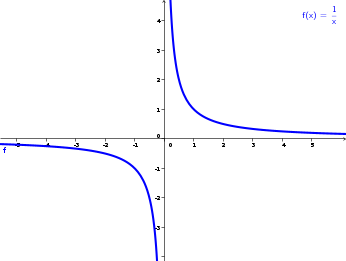
\includegraphics[width=0.65\linewidth]{chapters/chapter 5/1 over x.png}
\end{figure}

Օրինակ՝ $f(x) = \dfrac{1}{x}$ ֆունկցիայի գրաֆիկից երևում է, որ երբ $x$-ը մոտեցնում ենք $3$ կետին, ֆունկցիայի ընդունած արժեքները մոտենում են $\dfrac{1}{3}$-ին, հետևաբար՝ $\lim\limits_{x \to 3} \dfrac{1}{x}=\dfrac{1}{3}$:

Իսկ ի՞նչ կարող ենք ասել $0$ կետում սահմանի մասին։ Եթե $x$-ը $0$ կետին մոտեցնենք աջից, $f(x)$-ի արժեքները աճելով կձգտեն $+\infty$-ի, մինչդեռ եթե ձախից մոտենանք՝ կձգտեն $-\infty$-ի։ Սա նշանակում է, որ ֆունկցիան $0$ կետում սահման չունի։ Ավելին, եթե $x=3$-ում ֆունկցիան որոշված է՝ \marginnote{$f$-ը կարծես երկու իրար հետ կապ չունեցող ֆունկցիա լինի}ունի արժեք, ապա $x=0$-ում ֆունկցիան արժեք էլ չունի՝ որոշված չէ։ Նման դեպքում կասենք, որ $f$-ը $0$ կետում \textit{խզվող} է, իսկ մնացած կետերում՝ \textit{անընդհատ։}

\begin{definition}
Կասենք, որ $f$ ֆունկցիան \textbf{անընդհատ} է $a$ կետում, եթե
\begin{enumerate}
    \item $f$-ը $a$-ում որոշված է\marginnote{ունի արժեք}
    \item $\lim\limits_{x \to a} f(x)$ սահմանը գոյություն ունի\marginnote{ունի սահման}
    \item $\lim\limits_{x \to a} f(x) = f(a)$\marginnote{արժեք $=$ սահման}
\end{enumerate}
\end{definition}

Պատկերավոր ասած՝ տվյալ կետում ֆունկցիան անընդհատ է, եթե դրա գրաֆիկը հնարավոր է գծել՝ առանց գրիչը թղթից կտրելու։

\warning{Ֆունկցիան կարող է մի կետում անընդհատ լինել, մի ուրիշ կետում՝ խզվել։}

Անընդհատությունը շատ օգտակար հատկություն է, և գործնականում հանդիպող ֆունկցիաները, բարեբախտաբար, մեծ մասամբ անընդհատ են $(-\infty, \infty)$ ընկած բոլոր կետերում (ողջ $\R$-ում), կամ մեկ-երկու կետից բացի մնացած բոլոր կետերում,\marginnote{օրինակ՝ $\sqrt{x}$-ը կամ $\dfrac{1}{x}$-ը, որոնք ոչ բոլոր կետերում են որոշված} կամ էլ՝ բոլոր այն կետերում, որտեղ որոշված են։ 

Նշենք, որ եթե որևէ $a$ կետում $f$-ն ու $g$-ն անընդհատ են, ապա դրանք գումարելիս, հանելիս, բազմապատկելիս, բաժանելիս կամ թվով բազմապատկելիս ստացվող ֆունկցիաները՝
\begin{itemize}
    \item $f+g$
    \item $f-g$
    \item $f\cdot g$
    \item $\dfrac{f}{g}$ (եթե $g(a) \ne 0$)
    \item $cf$ ($c$-ն ցանկացած թիվ է)
\end{itemize}
նույնպես անընդհատ են այդ կետում։

\question{Կռահո՞ւմ եք, թե ինչպիսի տարածություն է կազմում $a$ կետում անընդհատ բոլոր ֆունկցիաների բազմությունը։}


\begin{figure}[t]
\centering %
\floatsetup{floatrowsep=qquad}
\begin{floatrow}[3]%
\ffigbox[\FBwidth]{\caption*{\centering անընդհատ\linebreak (բոլոր կետերում որոշված)}}{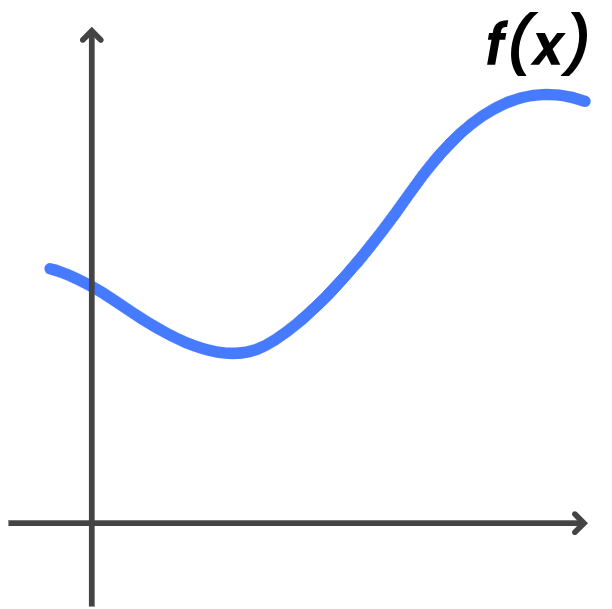
\includegraphics[width=0.4\textwidth]{chapters/chapter 5/continuity 1.png}}
\ffigbox[\FBwidth]{\caption*{\centering խզվող\linebreak (բոլոր կետերում որոշված)}}{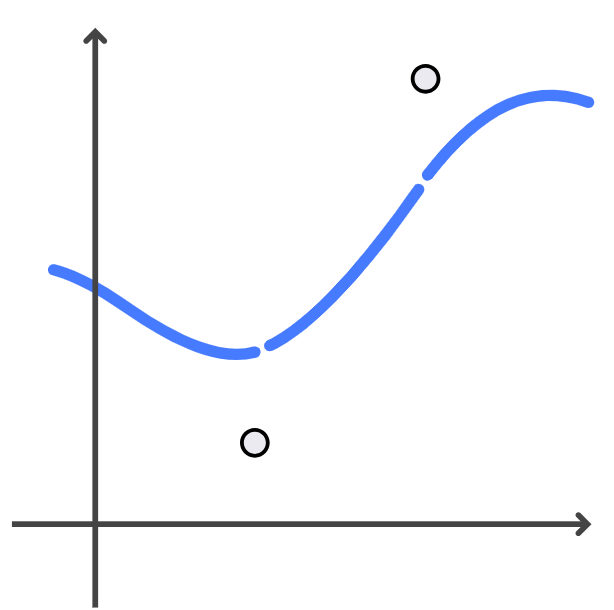
\includegraphics[width=0.4\textwidth]{chapters/chapter 5/continuity 2.png}}
\ffigbox[\FBwidth]{\caption*{\centering խզվող\linebreak (ոչ բոլոր կետերում որոշված)}}{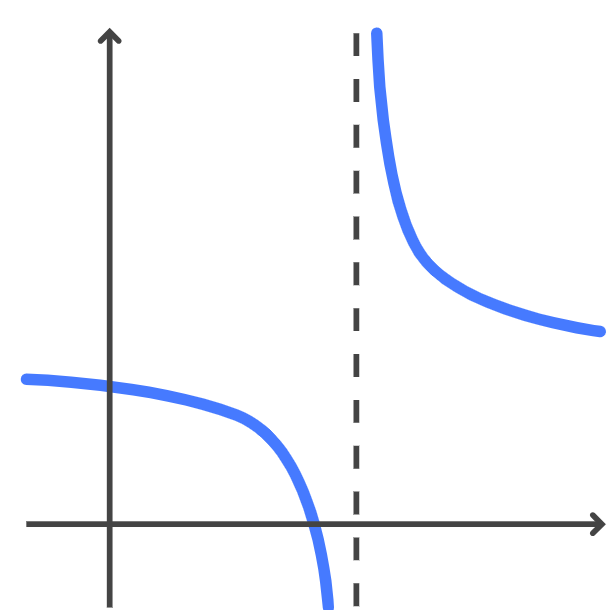
\includegraphics[width=0.4\textwidth]{chapters/chapter 5/continuity 3.png}}
\end{floatrow}
\end{figure}

Եթե ֆունկցիան բոլոր կետերում անընդհատ է (կամ գոնե՝ բոլոր այն կետերում, որոնցում որոշված է), ապա այն կարճ կասենք ուղղակի \textit{անընդհատ ֆունկցիա։} Անընդհատ ֆունկցիաներ են, օրինակ՝
\begin{itemize}
    \item հաստատուն ֆունկցիաները՝ $3$, $-8$
    \item գծային ֆունկցիաները՝ $3x+4$, $5x$, $y-x$
    \item առհասարակ բոլոր բազմանդամները՝ $x^2+7x-1$, $xy-y^4+z$
    \item արմատ պարունակող ֆունկցիաները՝ $\sqrt{x}$, $\sqrt[5]{x}$
    \item ցուցչային ու լոգարիթմական ֆունկցիաները՝\marginnote{որոշները ոչ բոլոր կետերում են որոշված} $2^x$, $e^{3x}$, $\ln{x}$
    \item եռանկյունաչափական ֆունկցիաներն ու դրանց հակադարձները՝ $\cos(3x)$, $\arcsin{x}$
\end{itemize}
և այլն։ Խզվող ֆունկցիաները հեշտ է պարզել՝ նայելով դրանց գրաֆիկին։ Եթե ինչ-որ կետի մոտենալիս ֆունկցիայի արժեքը տարբեր կողմերից տարբեր թվերի է ձգտում, կամ ասենք՝ գրաֆիկը մի որևէ կետում կտրվում է, ապա ֆունկցիան խզվող է։


\section{Ածանցյալ}

Պատկերացրեք՝ փոքրացել-դարձել եք կետ և ֆունկցիայի գրաֆիկի վրայով կարուսելի նման սահում եք վերև ու ներքև։ Ձեր ճանապարհը ֆունկցիայի գրաֆիկն է․ ինչ-որ ժամանակ դրանով կբարձրանաք դեպի վեր, հետո կսկսեք իջնել, հետո նորից բարձրանալ, երբեմն՝ ավելի մեծ արագությամբ կընթանաք, երբեմն՝ շարժումը կդանդաղի։

\begin{figure}[h]\label{local_extr}
    \centering
    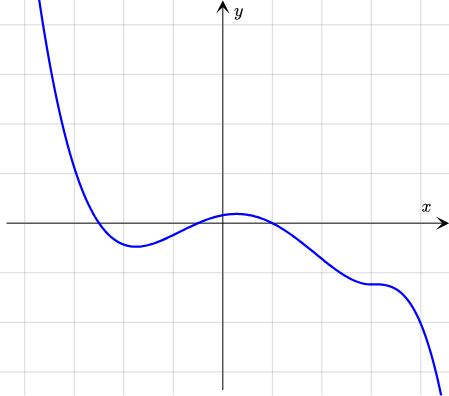
\includegraphics[width=0.6\linewidth]{chapters/chapter 5/just function.png}
\end{figure}

Բայց փաստացի՝ հիմա Դուք կետ չեք։ Գրաֆիկով մեկ սահել չեք կարող, փոխարենը պետք է բավարարվեք ֆունկցիայի բանաձևով։ Ինչպե՞ս կարող ենք բանաձևից ելնելով՝ պարզել, թե երբ ու ինչպես են տեղի ունենում ֆունկցիայի այս վայրիվերումները։

Նախ ֆիքսենք, թե գրաֆիկի ո՞ր կետում եք գտնվում, և փորձենք հաշվել այդ կետում Ձեր ունեցած արագությունը։ Ենթադրենք՝ գտնվում ենք ${x=a}$ \marginnote{ֆունկցիայի ընդունած արժեքը՝ $f(a)$} կետում։

\question{Ինչպե՞ս կհաշվեք, թե տնից խանութ գնալու ճանապարհին որքա՞ն է Ձեր մոտավոր արագությունը։}

Եթե այժմ $a$ կետից մի փոքր շարժվենք դեպի աջ կամ ձախ, ասենք՝ շատ չնչին $h$ չափով\marginnote{եթե ձախ ենք շարժվում, $h$-ը կվերցնենք բացասական}, ապա կհայտնվենք $f(a+h)$-ում, այսինքն՝ $h$ չափով քայլ կատարելու դեպքում կբարձրանանք/կիջնենք 
\[
f(a+h) - f(a)
\]
չափով։ Եթե հիմա այս փոփոխության չափը բաժանենք մեր կատարած քայլի վրա՝
\[
\frac{f(a+h) - f(a)}{h}
\]
կստանանք «միջին» կամ «միավոր» փոփոխության չափը ($a$ կետի շուրջն այս ու այն կողմ գնալիս)։

Վերջապես, քանի որ ուզում ենք չափել հենց $a$ կետում մեր շարժման արագությունը,\marginnote{$a$-ից հեռու $f$-ի արագությունը կարող է ավելի մեծ/փոքր լինել, բայց դա $a$-ում արագության վրա չպետք է ազդի} ապա պետք է կենտրոնանանք միայն $a$ կետին շատ մոտիկ շրջակայքի վրա։ Այլ կերպ ասած՝ ստիպենք, որ $h$-ը լինի շա՜տ փոքր՝
\[
\lim_{h\to 0} \frac{f(a+h) - f(a)}{h}
\]

Ինչ թիվ որ արդյունքում ստանանք, հենց դա էլ ցույց կտա $a$-ում մեր (այսինքն՝ $f$-ի գրաֆիկի աճել/նվազելու) արագությունը։ Այդ թիվը կոչվում է $a$ կետում $f$-ի \textit{ածանցյալ։}

\begin{definition}
Եթե հետևյալ սահմանը գոյություն ունի և անվերջ չէ՝\marginnote{կամ որ նույնն է՝ $\displaystyle \lim_{{x\to a}} \frac{f(x) - f(a)}{x-a}$}
\[
\lim_{h \to 0} \frac{f(a + h) - f(a)}{h}
\]
ապա այն կնշանակենք $f'(a)$-ով կամ $\dfrac{df}{dx}(a)$-ով և կանվանենք $f$ ֆունկցիայի \textbf{ածանցյալ} $a$ կետում։
\end{definition}

Եթե $f$-ն $a$-ում ունի ածանցյալ, ապա կասենք, որ այն \textit{ածանցելի} կամ \textit{դիֆերենցելի} է $a$ կետում։

\begin{example}
Դիտարկենք $f(x) = x^2$ ֆունկցիան։ Որևէ $x$ կետում դրա ածանցյալը հաշվելու համար գրենք՝
\[
f'(x) = \lim\limits_{{h \to 0}} \frac{(x + h)^2 - x^2}{h} =  \lim\limits_{{h \to 0}} \frac{x^2+2xh+h^2 - x^2}{h} = 2x
\]
Ուրեմն՝ ցանկացած $x$ կետում $f$-ի ածանցյալն է՝ $f'(x) = 2x$։
\end{example}

Եվս մեկ անգամ արձանագրենք, որ ֆունկցիայի ածանցյալը տվյալ կետում ցույց է տալիս այդ ֆունկցիայի \textit{փոփոխման արագությունը՝} որքան է փոխվում ֆունկցիայի արժեքը,\marginnote{որքան զգայուն է ֆունկցիան իր արգու\-մեն\-տի փոփոխության նկատմամբ} երբ նրա արգումենտը մի փոքր փոփոխում ենք։ Իհարկե, ֆունկցիան կարող է երբեմն արագանալ, երբեմն՝ դանդաղել, հետևաբար՝

\warning{Ածանցյալը տարբեր կետերում ընդունում է տարբեր ար\-ժեքներ․ $f'(x)$-ը ոչ թե ֆիքսված թիվ է, այլ $x$-ից կախված ֆունկցիա։}
\question{Որքան $x$-ը գնում է աջ, այնքան $f(x)=x^2$-ու ածանցյալը մեծանում է։ $f$-ի գրաֆիկին նայելով՝ ինչպե՞ս կմեկնաբանեք դա։}
Նշենք, որ եթե անընդհատությունը լավ հատկություն է, ապա դիֆերեն\-ցելիությունը էլ ավելի լավ հատկություն է։ Մասնավորապես,

\begin{theorem}
Եթե ֆունկցիան որևէ կետում դիֆերենցելի է, ապա նաև անընդհատ է այդ կետում։
\end{theorem}

Բայց հակառակը ճիշտ չէ․ կան ֆունկցիաներ, որոնք անընդհատ են, բայց դիֆերենցելի չեն։

\begin{example}
\begin{marginfigure}
    \centering
    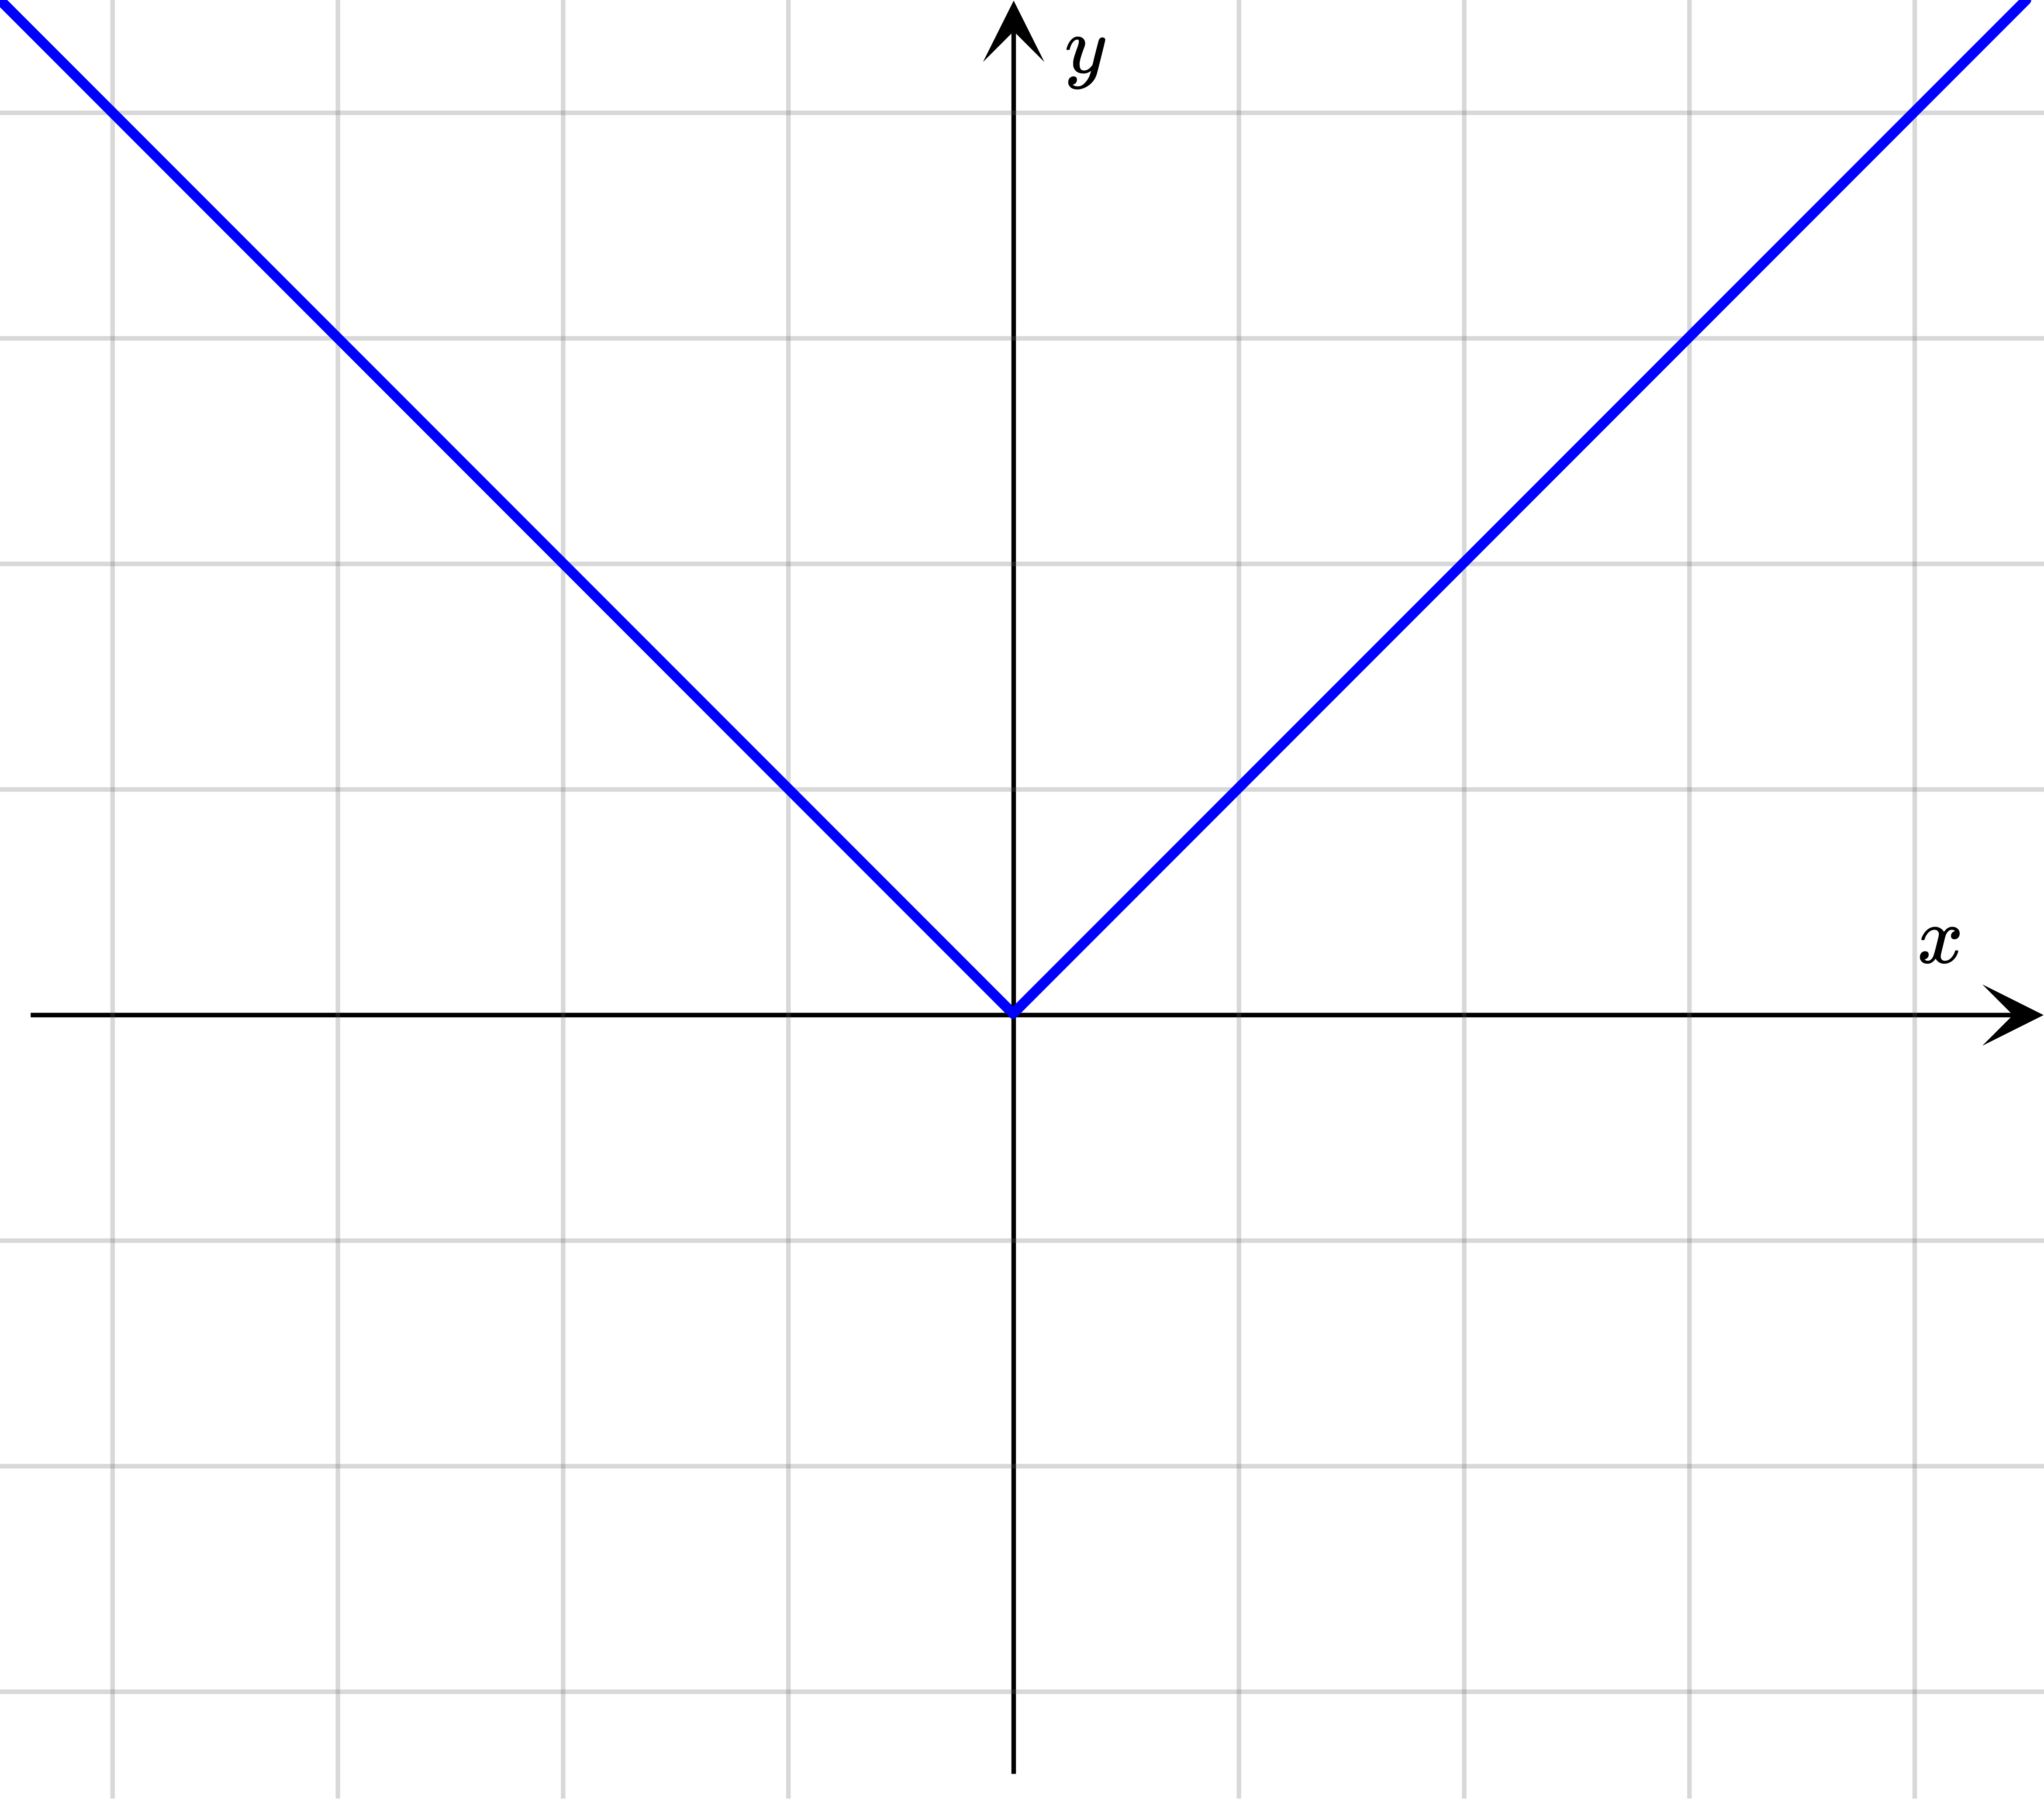
\includegraphics[width=1\linewidth]{chapters/chapter 5/abs(x).png}
    \caption*{կարծես երկու ֆունկցիաներ $0$ կետում կպցրած լինեն միմյանց, բայց ոչ այնքան սահուն ձևով}
\end{marginfigure}
$f(x)=|x|$ ֆունկցիան անընդհատ է, նրա ածանցյալը դրական $x$-երում $1$ է՝
\[
\lim_{h\to 0} \frac{|x+h|-|x|}{h}
=
\lim_{h\to 0} \frac{x+h-x}{h}
=
1
\]
բացասական կետերում՝ $-1$՝
\[
\lim_{h\to 0} \frac{|x+h|-|x|}{h}
=
\lim_{h\to 0} \frac{-(x+h)-x}{h}
=
-1
\]
Իսկ այ $x=0$ կետում ֆունկցիան ածանցյալ չունի, քանի որ եթե $0$-ին մոտենանք 

\begin{itemize}
    \item \item աջից՝ $h>0$, կունենանք՝ $\dfrac{|0+h|-|0|}{h}=\dfrac{h}{h}=1$
    \item ձախից՝ $h<0$, կունենանք՝ $\dfrac{|0+h|-|0|}{h}=\dfrac{-h}{h}=-1$
\end{itemize}

Ընդհանուր դեպքում $h$-ը $0$-ի ձգտելիս սահման չկա, հետևաբար $f$-ը $0$-ում դիֆերենցելի չէ։
\end{example}

Ինչպես կարող եք ենթադրել՝ նայելով գրաֆիկին, ածանցյալ չունենալու պատճառը $0$ կետում ուղղության շատ կտրուկ փոփոխությունն է։

\question{Որքա՞ն կլինի $f(x)=14$ հաստատուն ֆունկցիայի ածանցյալը։}

Նման եղանակով կարող ենք հաշվել մի քանի հաճախ հանդիպող ֆունկցիաների ածանցյալները․ \phantomsection \label{derivatives_list}
\begin{itemize}
    \item $(c)' = 0$ \marginnote[*+1]{հաստատունի ածանցյալը $ = 0$}
    \item $(x)' = 1$
    \item $(x^2)' = 2x$
    \item $(x^n)' = nx^{n-1}$ 
    % \marginnote{մասնավորապես՝\\$\left(\dfrac{1}{x}\right)'=\left(x^{-1}\right)'=-x^{-2}=-\dfrac{1}{x^2}$\\$\left(\sqrt{x}\right)'=\left(x^{1/2}\right)'=\dfrac{1}{2}x^{-1/2}=\dfrac{1}{2\sqrt{x}}$}
    \item $(e^x)' = e^x$
    \item $(a^x)' = a^x\ln a$
    \item $(\ln x)' = \dfrac{1}{x}$
    \item $(\sin x)'=\cos x$
    \item $(\cos x)'=-\sin x$
\end{itemize}
իսկ չորրորդ կանոնից մասնավորապես հետևում է, որ
\begin{itemize}
    \item $\left(\dfrac{1}{x}\right)'=\left(x^{-1}\right)'=-x^{-2}=-\dfrac{1}{x^2}$
    \item $\left(\sqrt{x}\right)'=\left(x^{1/2}\right)'=\dfrac{1}{2}x^{-1/2}=\dfrac{1}{2\sqrt{x}}$
\end{itemize}

\question{Ի՞նչ եք կարծում, որքա՞ն է $e^x + \cos x$-ի ածանցյալը։}

Արդեն հայտնի ֆունկցիաներից բաղկացած այլ ֆունկցիաների ածանց\-յալը հաշվելիս օգտակար են հետևյալ բանաձևերը․
\begin{itemize}
    \item $(cf)'=c\cdot f'$
    \item $(f + g)'=f' + g'$
    \item $(f - g)'=f' - g'$
    \item $(fg)'=f'g+fg'$
    \item $\left(\dfrac{1}{f}\right)'=-\dfrac{f'}{f^2}$ (եթե $f\ne 0$)
    \item $\left(\dfrac{f}{g}\right)'=\dfrac{f'g-fg'}{g^2}$ (եթե $g\ne 0$)\marginnote{այո, տարօրինակ են, բայց ի՞նչ արած}
\end{itemize}

Այժմ արդեն կարող ենք հաշվել այնպիսի ֆունկցիաների արագություն\-ներ, ինչպիսիք են՝ $x^2e^x$, $4x^3-3x+1$ կամ $\operatorname{tg}x=\dfrac{\sin x}{\cos x}$։ 

Իսկ ինչպե՞ս հաշվել $\sin(x^2)$ ֆունկցիայի ածանցյալը։ Այլ կերպ ասած՝ այն ֆունկցիայի, որը ստացվում է, երբ $\sin x$ ֆունկցիայի մեջ տեղադրում ենք $x^2$ ֆունկցիան ($x$-ի փոխարեն)՝ \marginnote[*+1]{այսպիսի ֆունկցիաները կոչվում են \textit{բարդ ֆունկցիաներ}}
\[
h(x) = \overbrace{\sin}^{{\color{myblue}\text{սրա մեջ}}}(\underbrace{x^2}_{{\color{myred}\text{տեղադրած սա}}}) = {\color{myblue} f}({\color{myred} g}(x))
\]
որտեղ $f$-ով ու $g$-ով նշանակել ենք համապատասխանաբար $\sin x$ և $x^2$ ֆունկցիաները։ Դե, այս դեպքում
\begin{enumerate}
    \item առանձին-առանձին հաշվում ենք $f(x)=\sin x$-ի և $g(x)=x^2$-ի ածանցյալները
    \item $f'(x)$-ի մեջ $x$-ի փոխարեն տեղադրում ենք $g(x)$-ը՝ $f'(g(x))$
    \item և ստացված թվերը բազմապատկում՝ $f'(g(x)) \cdot g'(x)$
\end{enumerate}

Ստացված բանաձևով որոշվում է բարդ ֆունկցիայի ածանցյալը՝
\[
h'(x) = (f(g(x)))' = f'(g(x)) \cdot g'(x)
\]
մասնավորապես՝ $(\sin(x^2))' = \cos(x^2) \cdot 2x$:

\question{Իսկ ինչի՞ է հավասար $(\sin x)^2$-ու ածանցյալը։}

Վերջապես, ոչինչ մեզ չի արգելում ածանցել $f'$ ֆունկցիան։ Իրոք, եթե ածանցում ենք $f$-ը, ստանում ենք դրա փոփոխման արագությունը ցույց տվող $f'$-ը, բայց այս $f'$-ն ինքը ֆունկցիա է, ուրեմն ինչո՞ւ չածանցել։ Եթե $f'$-ը ցույց է տալիս $f$-ի արագությունը, $f'$-ի ածանցյալը ցույց կտա 
\[
\hspace{-1em}f'\text{-ի արագությունը} = f\text{-ի արագության արագությունը} = f\text{-ի արագացումը}
\]

$f'$-ի ածանցյալը նշանակում ենք $f''$-ով, $f''$-ինը՝ $f'''$-ով, և այդպես շարունակ։ $15$-րդ կարգի ածանցյալը նշանակում ենք \st{$f'''''''''''''''$-ով} $f^{(15)}$-ով, և այլն։


\section{Ածանցյալի նշանը}

Երբ ինչ-որ կետում ֆունկցիայի ածանցյալը, ասենք, $100$ է, նշանակում է՝ այդ կետի հարևանությամբ ֆունկցիայի աճելու արագությունը բա\-վա\-կանին մեծ է․ մի փոքր չափով աջ \marginnote{նորից պատկերացրեք՝ կետ եք, գրա\-ֆի\-կի վրա նստած սլանում եք վերև-ներքև} գնալիս ֆունկցիան մոտավորապես $100$ այդքանով մեծանում է։ Եթե ինչ-որ պահի ածանցյալը դառնա $10$, նշանակում է՝ ֆունկցիայի աճելու արագությունը փոքրացավ․ արդեն ավելի դանդաղ է աճում։ Եթե ավելի ուշ դարձավ $5$, ուրեմն աճելու արագությունը էլ ավելի նվազեց։ Իսկ այ եթե հաջորդ պահին ածանցյալը դառնա $-5$, ապա...

\question{Ի՞նչ եք կարծում, ի՞նչ կնշանակի դա։}

․․․ֆունկցիան այլևս ոչ թե աճում է, այլ՝ \textit{նվազում։} 

\begin{definition}
Կասենք, որ $f(x)$ ֆունկցիան $a$ կետում \textbf{աճող} է, եթե $a$-ին շատ մոտիկ\marginnote{կարող ենք ասել՝ եթե 
\[a-\delta < c < a < b < a+\delta\]
ինչ-որ մի փոքր $\delta$-ի համար} ցանկացած $b$, $c$ կետերում
\[
f(c) < f(a) < f(b) \qquad \text{եթե } c<a<b
\]
և որ այն \textbf{նվազող} է, եթե
\[
% f(c)\le f(a) \le f(b) \qquad \text{եթե } c<a<b
f(c) > f(a) > f(b) \qquad \text{եթե } c<a<b
\]
\end{definition}

\begin{figure}[h]
    \centering
    \subfloat{{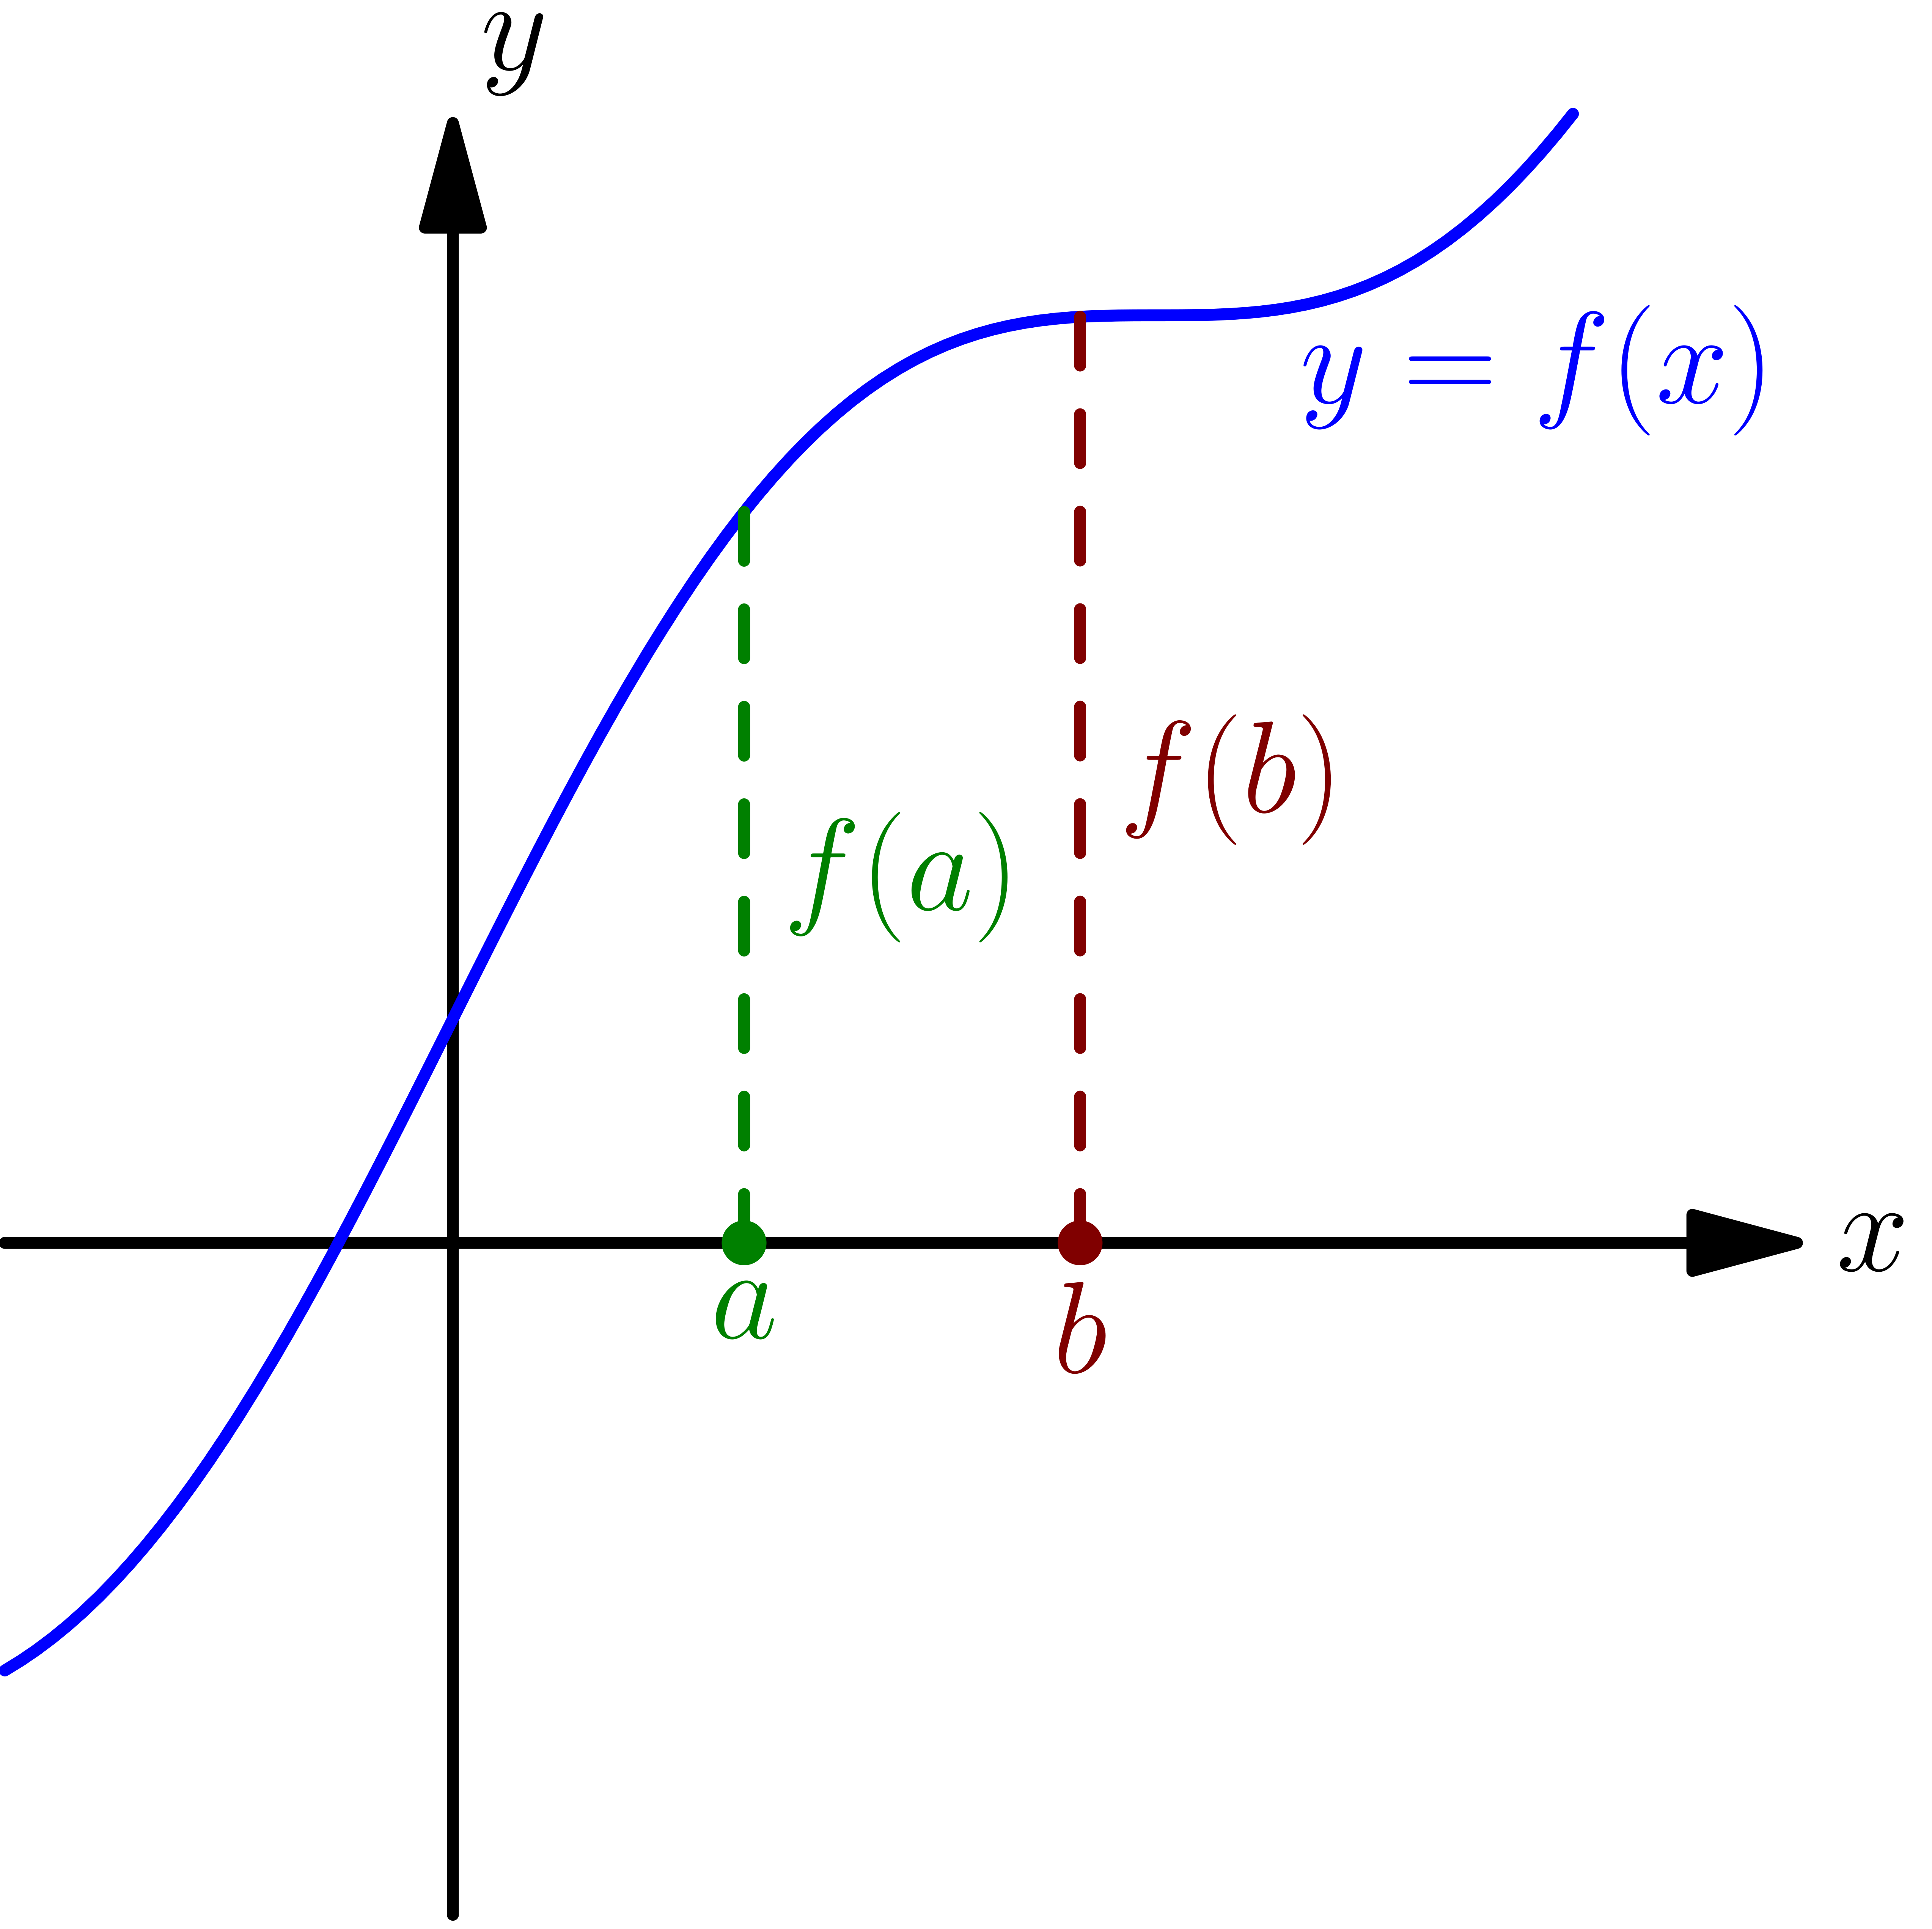
\includegraphics[width=0.4\linewidth]{chapters/chapter 5/increasing.png} }}%
    \qquad
    \subfloat{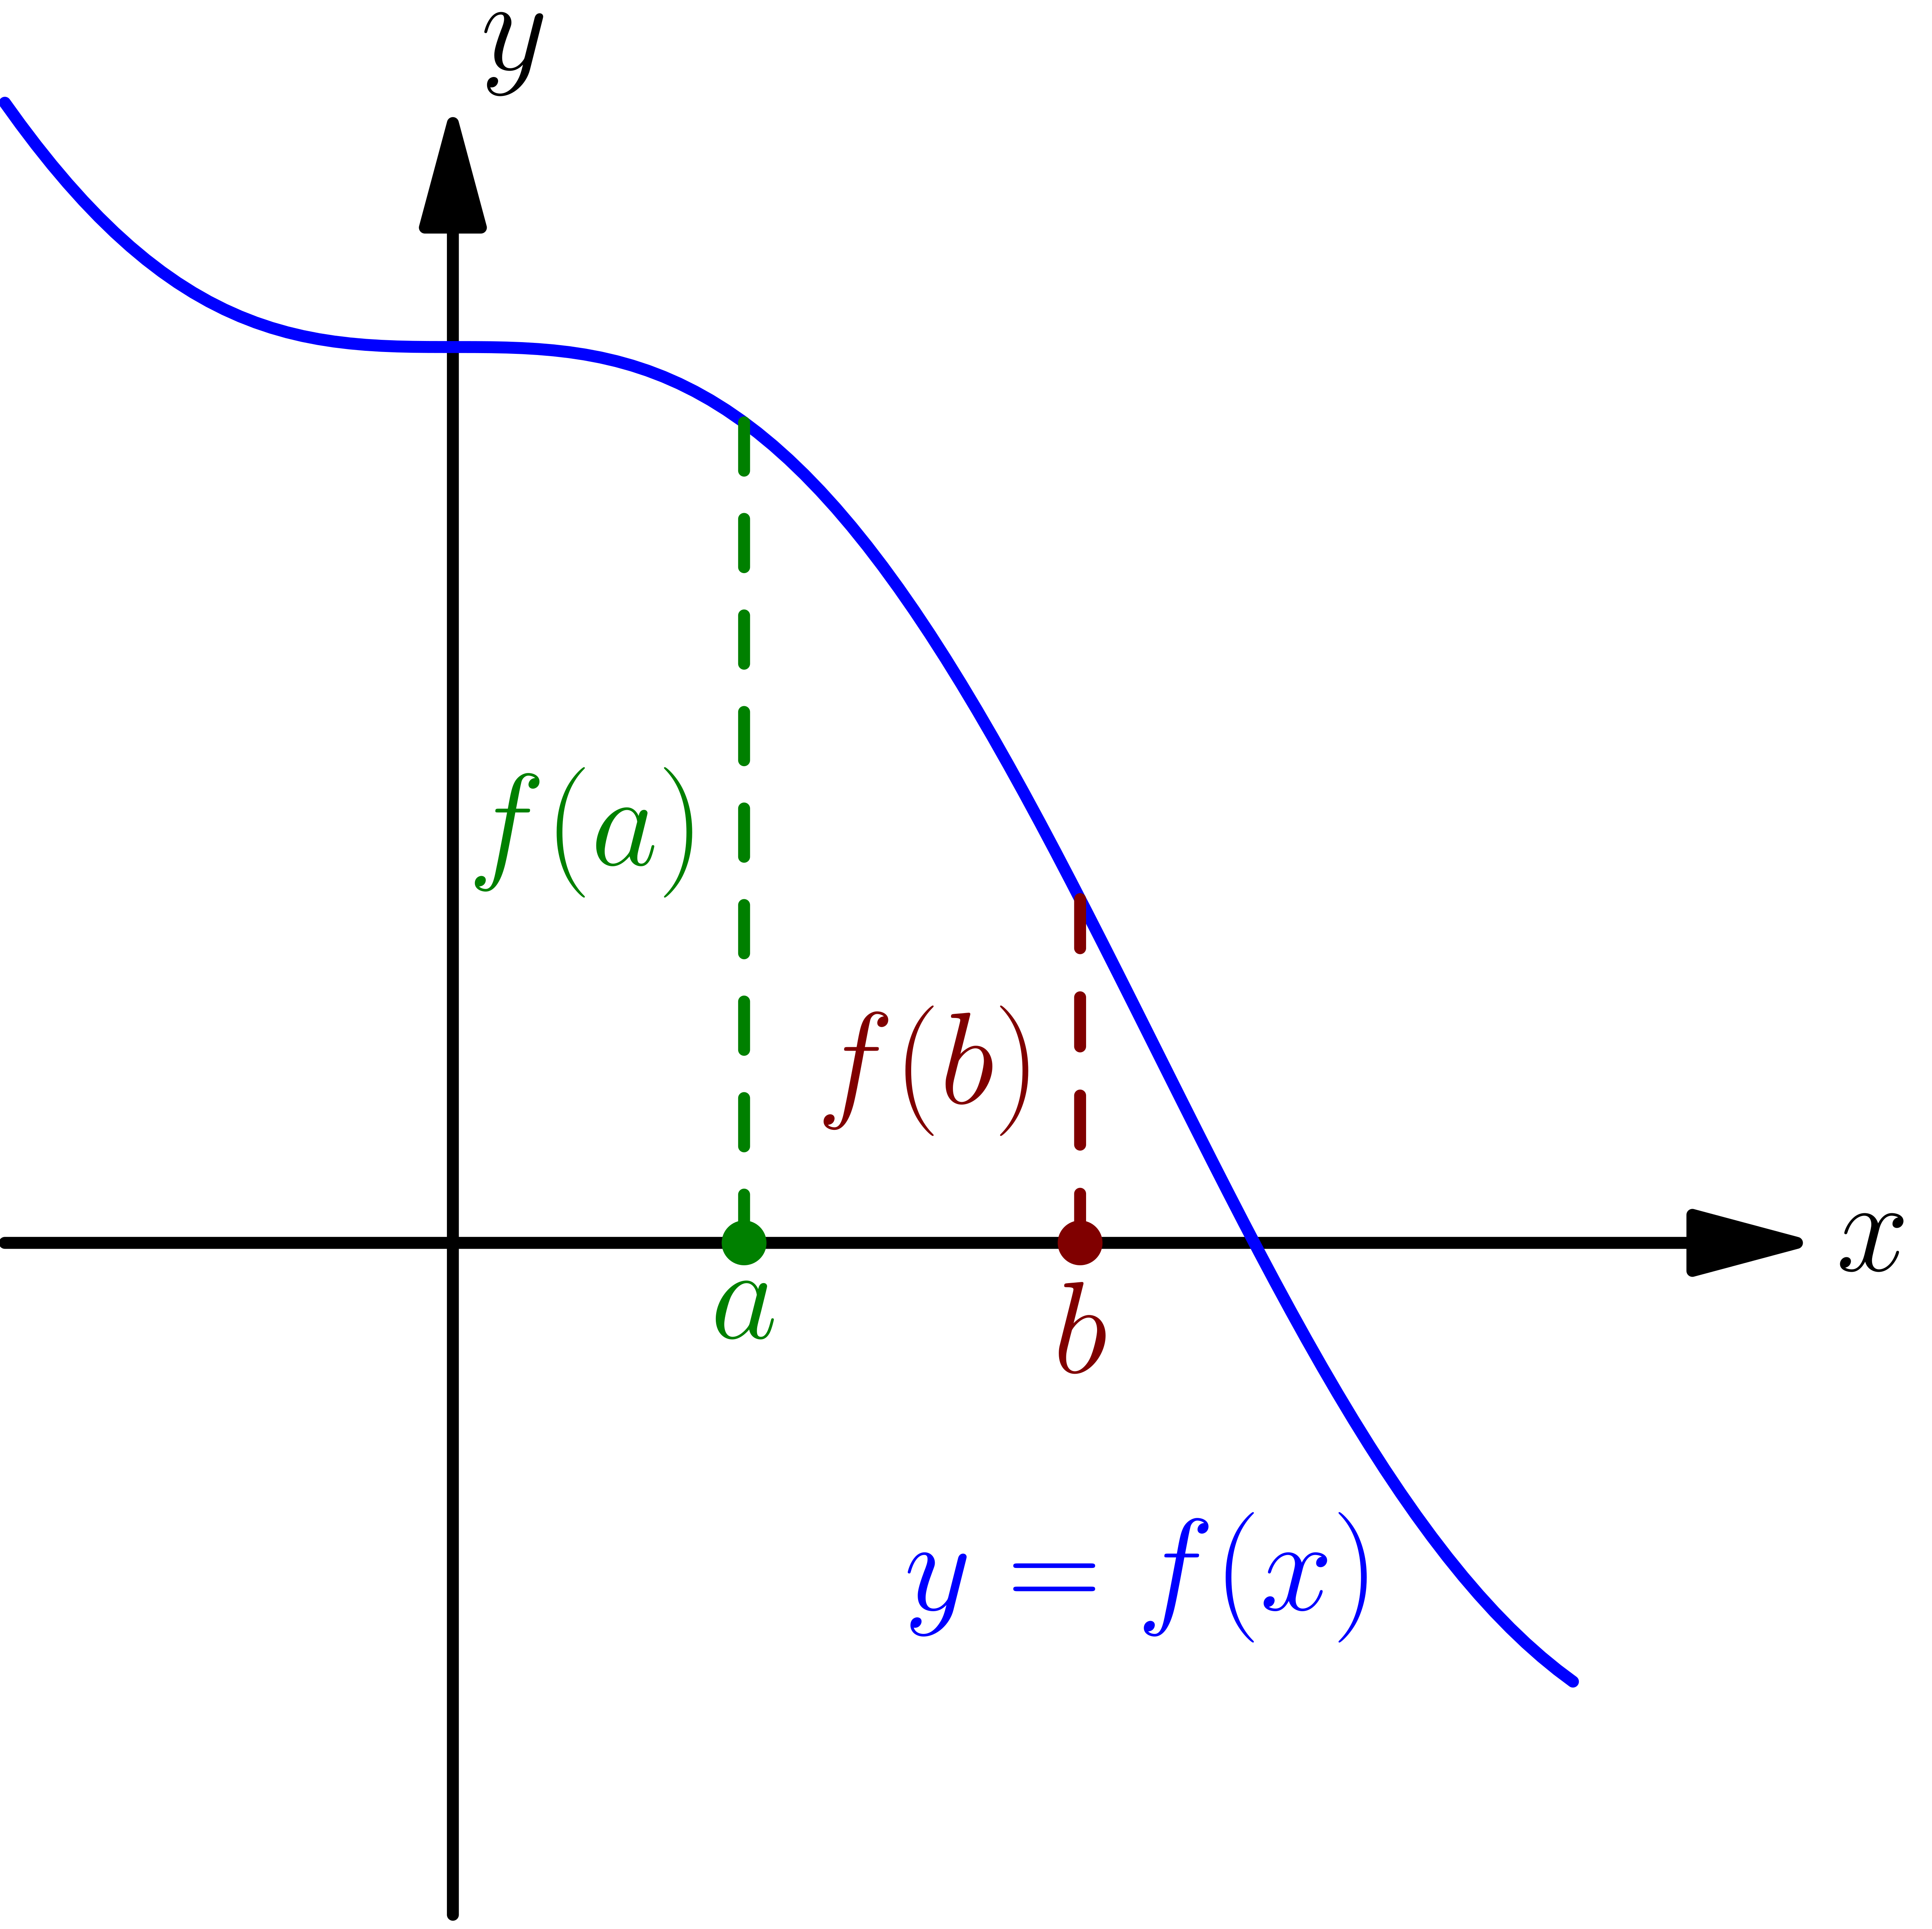
\includegraphics[width=0.4\linewidth]{chapters/chapter 5/decreasing.png}} %
    % \caption*{աճողը և նվազողը}
\end{figure}

Նման ձևով կարող ենք սահմանել նաև \textit{չնվազող՝}
\[f(c) \le f(a) \le f(b) \qquad \text{եթե } c<a<b\]
և \textit{չաճող՝}
\[f(c) \ge f(a) \ge f(b) \qquad \text{եթե } c<a<b\]
ֆունկցիայի գաղափարները, որոնք ներառում են նաև հավասարության դեպքերը։

\question{Կարո՞ղ եք գծել/գրել այնպիսի ֆունկցիա, որը $0$-ում աճող է, $1$-ում՝ նվազող: Ո՞ր ֆունկցիան է և՛ չաճող, և՛ չնվազող։}

Յուրաքանչյուր կետում կարող ենք պարզել՝ ֆունկցիան աճում է, թե նվազում, նայելով միայն նրա ածանցյալի նշանին։\marginnote[*+3]{դրական արագություն $=$ աճող\\բացասական արագություն $=$ նվազող}

\begin{theorem}
Ենթադրենք $f$ ֆունկցիան դիֆերենցելի է $a$ կետում։ Ուրեմն
\begin{itemize}
    \item եթե $f'(a) > 0$, ապա $f$-ն $a$-ում աճող է
    \item եթե $f'(a) < 0$, ապա $f$-ն $a$-ում նվազող է
    \item եթե $f'(a) \ge 0$, ապա $f$-ն $a$-ում չնվազող է
    \item եթե $f'(a) \le 0$, ապա $f$-ն $a$-ում չաճող է
\end{itemize}
\end{theorem}

\question{Ներքևում բերված ֆունկցիայի ածանցյալը ո՞ր կետերում է դրական։ Իսկ որոնցո՞ւմ է բացասական։}

\begin{figure}[h]
    \centering
    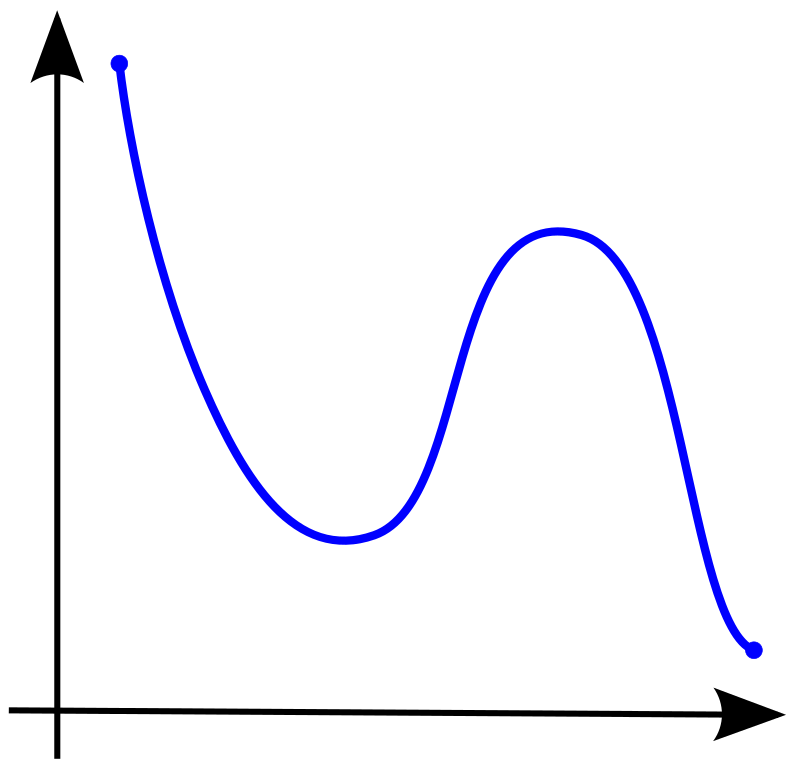
\includegraphics[width=0.4\linewidth]{chapters/chapter 5/just another function.png}
\end{figure}

\question{Պատկերացրեք՝ \hyperref[apricot]{\color{OliveGreen}ծիրանի գինը} դրել եք $x=4$։ Կմեծանա՞, թե՞ կփոքրանա խանութի եկամուտը, եթե գինը մի փոքր բարձրացնեք։}

\section{Էքստրեմումի խնդրի լուծումը}\label{single_var_extrema}

Փաստորեն արդեն գիտենք, թե ինչպես ածանցյալի նշանից հասկանալ՝ գինը բարձրացնե՞լ, թե՞ իջեցնել՝ եկամուտը մեծացնելու համար։ Իսկ ինչպե՞ս պարզել, թե որ գնի դեպքում է եկամուտն ամենամեծը, այլ կերպ ասած՝ ո՞ր $x$ կետում է ֆունկցիան ընդունում իր ամենամեծ արժեքը։ 

\question{Ենթադրենք $f$ ֆունկցիան իր ամենամեծ արժեքը ընդունում է $a$ կետում։ Ի՞նչ կարող եք ասել այդ կետում $f$-ի ածանցյալի մասին։}

\marginnote[*+1]{իսկ այն կետը, որում ֆունկցիան ընդու\-նում է այդ արժեքը, կանվանենք գլո\-բալ մաքսիմումի/մինիմումի \textit{կետ}}Պայմանավորվենք ֆունկցիայի ընդունած ամենամեծ արժեքն անվանել ֆունկցիայի \textit{գլոբալ մաքսիմում,} ամենափոքրը՝ \textit{գլոբալ մինիմում,} իսկ այս երկուսը միասին՝ \textit{գլոբալ էքստրեմումներ։} 

\warning{Որոշ ֆունկցիաներ ունեն գլոբալ մաքսիմում, որոշ ֆունկցիաներ՝ ոչ։}

\begin{example}\label{extrema_example}
Գծելով հետևյալ ֆունկցիաների գրաֆիկները՝ կնկատեք, որ
\begin{itemize}
    \item $f(x)=x^2$ ֆունկցիան ունի 
    \begin{itemize}
        \item[-] գլոբալ մինիմում $x=0$ կետում
        \item[-] գլոբալ մաքսիմում չունի
    \end{itemize}
    
    \item $f(x)=-x^2$ ֆունկցիան ունի
    \begin{itemize}
        \item[-] գլոբալ մաքսիմում $x=0$ կետում
        \item[-] գլոբալ մինիմում չունի    \marginnote{այստեղ կարող էին լինել գրաֆիկներ, բայց փոխարենը կա \href{https://www.desmos.com}{հղում}}
    \end{itemize}
    
    \item $f(x)=25x^4 - 50x^2 + 16$ ֆունկցիան ունի
    \begin{itemize}
        \item[-] գլոբալ մինիմում $x=-1$ և $x=1$ կետերում
        \item[-] գլոբալ մաքսիմում չունի
    \end{itemize}
        
    \item $f(x)=\dfrac{\sin{x}}{x}$ ֆունկցիան ունի
    \begin{itemize}
        \item[-] գլոբալ մինիմում $x \approx -4.49$ և $x \approx 4.49$ կետերում
        \item[-] գլոբալ մաքսիմում $x=0$ կետում
    \end{itemize}
    
    % \item $f(x)=\cos{x}$ ֆունկցիան ունի 
    % \begin{itemize}
    %     \item[] գլոբալ մինիմում $x \approx -4.49$ և $x \approx 4.49$ կետերում
    %     \item[] գլոբալ մաքսիմում $x=0$ կետում
    % \end{itemize}
    
    % գլոբալ մինիմում $x = \pm\pi, \pm3\pi, \pm5\pi, \dots$ կետերում, իսկ գլոբալ մաքսիմում՝ $x=0, \pm2\pi, \pm4\pi, \dots$ կետերում
    \item $f(x)=5$ ֆունկցիան միշտ ընդունում է նույն արժեքը, որը և՛ գլոբալ մաքսիմումն է, և՛ գլոբալ մինիմումը
    
    \item $f(x)=3x+1$ ֆունկցիան չունի ոչ գլոբալ մաքսիմում, ոչ գլոբալ մինիմում
\end{itemize}

Ի՞նչ կարող եք ասել $f(x)=\cos x$-ի գլոբալ էքստրեմումների մասին։
\end{example}

Իսկ ինչո՞ւ ենք շեշտում «գլոբալ», մի՞թե կան այլ մինիմումներ։ Հիշենք նախորդ բաժնում պատկերված \hyperref[local_extr]{\color{OliveGreen}այս} ֆունկցիան։ Քանի որ այն աջ գնալիս շարունակ փոքրանում է՝ ընդունելով ավելի ու ավելի փոքր արժեքներ, ապա այն գլոբալ մինիմում չունի։ Սակայն նկատենք, որ $x\approx -2$ կետի մոտակայքում ֆունկցիան մի պահ նվազելով իջնում է ներքև, ապա սկսում դանդաղ բարձրանալ վերև, ինչի արդյունքում առաջանում է մի փոքր փոսիկ։ 

\begin{marginfigure}
    \centering
    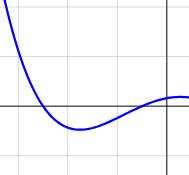
\includegraphics[width=0.6\linewidth]{chapters/chapter 5/zoomed function.png}
    \caption*{կամ այնքան մոտեցնենք ({\rm zoom} անենք), որ միայն այդքան մասը երևա}
\end{marginfigure} Հենց այդ փոսիկը կոչվում է ֆունկցիայի \textit{լոկալ մինիմում՝} այն իմաստով, որ եթե ֆունկցիան կտրենք, ասենք, $-3$ և $-1$ կետերի միջև ու նայենք ստացված փոքր տեղամասին, ապա կունենանք լոկալ մասշտաբով ամենափոքր արժեք։ Նույն ձևով՝ $x \approx 0.5$ կետի մոտակայքում ունենք «փոքրիկ» լոկալ մաքսիմում։ 

Ավելի պատկերավոր՝ Ջոմոլունգման գլոբալ մաքսիմում է, Մասիս սարը՝ լոկալ մաքսիմում։ Գլոբալ մաքսիմումն, իհարկե, կարևոր է, բայց ինչպես կտեսնենք, լոկալ մաքսիմումները նույնպես չարժի աչքաթող անել։

\begin{definition}
Կասենք, որ $f$-ը $a$ կետում ընդունում է \textbf{լոկալ մաքսիմում} (մինիմում), եթե բավականաչափ փոքր $(a-\delta, a+\delta)$ միջակայքի կետերում $f$-ի ամենամեծ (ամենափոքր) արժեքը $f(a)$-ն է։
\end{definition}

Կամ այլ կերպ ասած՝ եթե գոյություն ունի այնպիսի $\delta > 0$ թիվ, որ եթե $a - \delta < x < a + \delta$, ապա $f(x) \le f(a)$ (լոկալ մինիմումի դեպքում՝ $\ge$):

\begin{figure}[t]
    \centering
    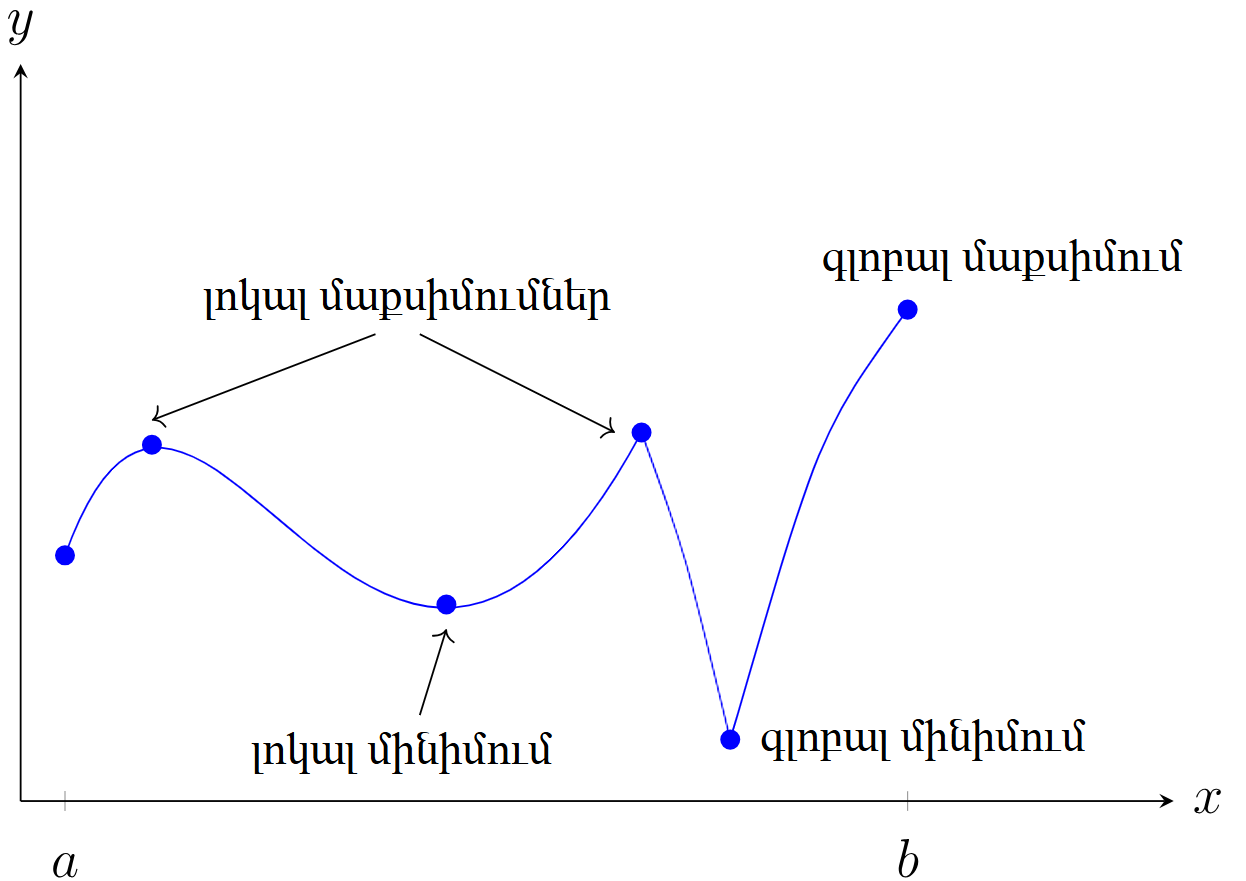
\includegraphics[width=0.65\linewidth]{chapters/chapter 5/extrema.png}
\end{figure}

\question{Որո՞նք են \hyperref[extrema_example]{\color{OliveGreen}նախորդ օրինակի} ֆունկցիաների լոկալ էքստրե\-մում\-ները (եթե իհարկե կան)։}

Բնականաբար, ամեն մի գլոբալ էքստրեմում նաև լոկալ էքստրեմում է, իսկ այ հակառակը՝ ոչ միշտ է ճիշտ։ Վերևում տեսել ենք, որ հնարա\-վոր է՝ ֆունկցիան ընդհանրապես չունենա գլոբալ կամ նույնիսկ լոկալ մաքսիմում/մինիմում (քանի որ, օրինակ, միշտ ավելի ու ավելի մեծ/փոքր արժեքներ է ընդունում)։ Նշենք միայն, որ եթե $x$-երը սահմանա\-փակենք ինչ-որ մի փակ (այսինքն՝ $[a, b]$ տեսքի)\marginnote{փակ $=$ ծայրակետերը ներառյալ} միջակայքում, ապա երաշխավորված է, որ այդքան տեղում կունենանք և՛ գլոբալ մինիմում, և՛ գլոբալ մաքսիմում․

\begin{theorem}
Եթե $f$-ն անընդհատ ֆունկցիա է, ապա այն ցանկա\-ցած $[a, b]$ միջակայքում ունի գլոբալ մաքսիմում և մինիմում։
\end{theorem}

Վերջապես ինչպե՞ս գտնենք ֆունկցիայի լոկալ կամ գլոբալ էքստրեմում\-ները։ Պատասխանը կրկին թաքնված է ֆունկցիայի ածանցյալի նշանի մեջ։ Ենթադրենք՝ ինչ-որ $a$ կետում $f$ ֆունկցիան ընդունում է լոկալ մինիմումի արժեք, այսինքն՝ լոկալ իմաստով $a$-ի շրջակայքում $f(a)$-ից փոքր արժեք չկա։ Լավ, ուրեմն կարո՞ղ է $a$ կետում $f$-ի ածանցյալը լինել բացասական։ 

\newpage

Եթե այն բացասական լինի, ապա $f$-ը $a$-ում պետք է լինի նվազող, այսինքն՝ մի փոքր առաջ գնալով ($a$-ից աջ՝ ինչ-որ մի $a+\delta$ կետում) ֆունկցիայի արժեքը կլինի ավելի փոքր, քան $a$-ում։ Ինչը, սակայն, բացառված է, քանի որ $a$-ն լոկալ մինիմումի կետ է․ նշանակում է $f'(a)$-ն բացասական չէ՝ $f'(a) \ge 0$: 

\question{Կարո՞ղ է $f'(a)$-ն լինել դրական։}

Ենթադրելով, որ հարցին պատասխանեցիք «ոչ» և նմանատիպ ձևով ապացուցեցիք դա, ֆիքսենք՝ $f'(a) \le 0$: Ուրեմն միակ հնարավոր տարբերակը մնաց՝ կա՛մ $f$-ը $a$ կետում ընդհանրապես ածանցյալ չունի, կա՛մ էլ եթե ունի, ապա $f'(a) = 0$։ Այդպիսի կետերին անվանում ենք \textit{կրիտիկական կետեր։}

\begin{theorem}
\marginnote{այսինքն՝ եթե կա $f'(a)$, ապա $f'(a)=0$}Եթե $a$-ն $f$-ի լոկալ կամ գլոբալ էքստրեմումի կետ է, ապա այն կրիտիկական կետ է։
\end{theorem}

\warning{Կրիտիկական կետ լինելը դեռ չի նշանակում, որ կետը էքստրեմումի կետ է։}

\begin{example}
Գծենք հետևյալ երեք ֆունկցիաների գրաֆիկները․
\begin{itemize}
\item $f_1(x)=x^2$, որի համար $x=0$-ն մինիմումի կետ է։ Իրոք՝
\[ f_1'(x)=2x,\qquad f_1'(0)=0 \]

\item $f_2(x)=-x^2$, որի համար $x=0$-ն մաքսիմումի կետ է՝
\[ f_2'(x)=-2x,\qquad f_2'(0)=0 \]

\item $f_3(x)=x^3$, որի համար $x=0$-ն ոչ մինիմումի, ոչ մաքսիմումի կետ է, մինչդեռ՝
\[ f_3'(x)=3x^2,\qquad f_3'(0)=0 \]
\end{itemize}
\end{example}

Փաստորեն $f'(x)=0$ պայմանը անհրաժեշտ է, բայց \textit{բավարար չէ․} ամեն կրիտիկական կետ չէ, որ լոկալ էքստրեմումի կետ է։ Երրորդ ֆունկցիայի դեպքում, օրինակ, ածանցյալի զրո լինելը նշանակում էր՝ ֆունկցիան աճելով եկավ, արագությունը նվազեցրեց, դարձրեց $0$, բայց հետո նորից սկսեց մեծացնել ու շարունակեց աճել (այլ ոչ թե սկսեց նվազել)։

Լավ, բա ի՞նչ անենք։ Պատկերացրեք՝ կրկին գրաֆիկը նստած իջնում եք դեպի ֆունկցիայի լոկալ մինիմումի կետը։ Քանի դեռ չեք հասել այդ կետին, արագությունը բացասական է (կամ առնվազն՝ ոչ դրական), որովհետև իջնում եք։ Հասնելով այդ կետին՝ արագությունը դառնում է $0$ (կրիտիկական կետ է)։ Ի՞նչ է լինում, երբ այդ կետը անցնում ու գնում եք առաջ։ Քանի որ լոկալ մինիմումի կետն անցել եք, ապա ֆունկցիայի գրաֆիկը պետք է բարձրանա․ արագությունը ոչ բացասական է։ Ուրեմն՝

\newpage


\begin{theorem}
\begin{marginfigure}
    \centering
    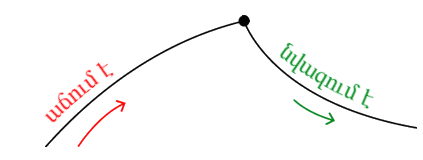
\includegraphics[width=0.8\linewidth]{chapters/chapter 5/derivative test.png}
\end{marginfigure}Եթե $f$-ը դիֆերենցելի է $a$ կետի մի որևէ $(a-\delta, a+\delta)$ շրջակայքում,
\begin{itemize}
    \item \item եթե $a$ կետից ձախ $f'(x) > 0$, իսկ $a$-ից աջ՝ $f'(x) < 0$, ապա $a$-ն լոկալ մաքսիմումի կետ է
    \item եթե $a$ կետից ձախ $f'(x) < 0$, իսկ $a$-ից աջ՝ $f'(x) > 0$, ապա $a$-ն լոկալ մինիմումի կետ է
    \item եթե $a$ կետից աջ և ձախ $f'(x)$-ի նշանը նույնն է, ապա $a$-ն լոկալ էքստրեմումի կետ չէ
\end{itemize}
\end{theorem}

\question{Ինչպե՞ս կարտահայտեք $f'$-ի նշանի՝ դրականից բացասական դառնալը՝ օգտվելով $f''$-ից։}

Այն դեպքում, երբ հարմար չէ հաշվել $f'$-ը/հետազոտել դրա նշանը, բայց փոխարենը հեշտ է գտնել $f$-ի երկրորդ կարգի ածանցյալը, կարող ենք օգտվել հետևյալ թեորեմից․

\begin{theorem}
Եթե $f'(a)=0$ և
\begin{itemize}
    \item $f''(a) > 0$, ապա $a$-ն լոկալ մինիմումի կետ է
    \item $f''(a) < 0$, ապա $a$-ն լոկալ մաքսիմումի կետ է
\end{itemize}
\end{theorem}

Ուշադրություն դարձնենք, որ թեորեմը չի պատասխանում այն հարցին, թե ինչ է տեղի ունենում, երբ $f''(a)=0$: Այդ դեպքում այս թեորեմն անօգուտ է, բայց կարելի է օգտվել նախորդ թեորեմից։


\bigskip 

\begin{theory}
.
\begin{itemize}
\item կարդալ [{\rm Stewart}], 87-91 (սահման), 118-121 (անընդհատու\-թյուն), 146-148, 154-161 և 199-201 (ածանցյալ), 274-279 (էքստրեմումներ) էջերը  
\item ըստ ցանկության՝ [{\rm Stewart}], 99-101, 174-180, 184-189, 290-292 էջերը
\item դիտել  {\rm 3b1b}-ի \href{https://www.3blue1brown.com/lessons/essence-of-calculus}{1-ին}, \href{https://www.3blue1brown.com/lessons/derivatives}{2-րդ} և \href{https://www.3blue1brown.com/lessons/limits}{8-րդ} տեսադասերը մաթանալիզից 
\item ըստ ցանկության՝ նաև \href{https://www.3blue1brown.com/lessons/epsilon-delta}{9-րդը}
\item կարելի է նաև գտնել լուծված վարժություններ \href{https://tutorial.math.lamar.edu/Classes/CalcI/CalcI.aspx}{այստեղ}
\end{itemize}
\end{theory}

\newpage

\section{Խնդիրներ}

\begin{problem}
Ունի՞ արդյոք հաջորդականությունը սահման (երբ $n\to\infty$)։ Եթե այո, ապա գտեք այն․

\begin{enumerate}[label={\alph*}․]
\item $\dfrac{3-n}{2}$

\item $\dfrac{4\sqrt{n}}{n^3}$

\item $\dfrac{n-1}{n^2-1}$

\item $1^n$

\item $0.4^n$

\item $(-4)^n$

\item որպես առաջին անդամ՝ վերցրեք ցանկացած թիվ, \\որպես երկրորդ անդամ՝ վերցրեք առաջինը բաժանած $1.5$-ի, \\ապա՝ երկրորդը բաժանած $1.5$-ի, և այդպես շարունակ

\item $a_1=1$, \\$a_2 = \dfrac{a_1}{7}$-ում ստորակետից հետո գրված առաջին թվանշանը, \\$a_3= \dfrac{a_2}{7}$-ում ստորակետից հետո գրված առաջին թվանշանը,
\\$\dots$

\end{enumerate}

\hint{Որպեսզի զգաք, թե ինչպես է փոխվում հաջորդականու\-թյու\-նը, գրեք դրա առաջին մի քանի անդամները։ Վերջին կետում օգտվեք հաշվիչից։}
\end{problem}


\begin{problem}
Սահմանների մասին \hyperref[limit_properties]{\color{OliveGreen}թեորեմում} ոչինչ չէինք կարող ասել $\dfrac{a_n}{b_n}$-ի սահմանի մասին, երբ $\lim\limits_{n\to\infty} b_n = 0$։ Կարո՞ղ եք բերել այնպիսի $a$ և $b$ հաջորդականությունների օրինակներ, որոնց համար $\lim\limits_{n\to\infty} a_n = 0$, $\lim\limits_{n\to\infty} b_n = 0$, բայց
\begin{enumerate}[label={\alph*}․]
\item $\lim\limits_{n\to\infty} \dfrac{a_n}{b_n} = 1$

\item $\lim\limits_{n\to\infty} \dfrac{a_n}{b_n} = -5$

\item $\lim\limits_{n\to\infty} \dfrac{a_n}{b_n} = 0$

\item $\lim\limits_{n\to\infty} \dfrac{a_n}{b_n} = +\infty$

\item $\lim\limits_{n\to\infty} \dfrac{a_n}{b_n}$ գոյություն չունի
\end{enumerate}
\end{problem}


\begin{problem}
Հետևյալ ֆունկցիաները բաղկացած են $x=2$ կետում իրար «սոսնձած» երկու առանձին ֆունկցիաներից։ Կարո՞ղ եք գտնել $c$-ի այնպիսի արժեք, որի դեպքում ֆունկցիան անընդհատ լինի $2$-ում։\marginnote[*+2.5]{\href{https://www.desmos.com/calculator/c3047befa7}{սկզբից փորձեք աչքաչափով}}

\begin{enumerate}[label={\alph*}․]
\item \marginnote[*+2]{\href{https://www.desmos.com/calculator/8eb756f334}{սա նույնպես}} $f(x)=\begin{cases} 3x-5& \text{եթե }x<2 \\  x^2+c& \text{եթե }x \ge 2 \end{cases}$

\item $
f(x)=\begin{cases} x^3+1& \text{եթե } x<2 \\  cx^2& \text{եթե } x \ge 2 \end{cases} $ 

\item $
f(x)=\begin{cases} -7& \text{եթե } x<2 \\ c& \text{եթե } x=2 \\  4+3\sin(\pi x)& \text{եթե } x>2 \end{cases} $
\bigskip

\item $
f(x)=\begin{cases} {\dfrac{x^2-x-2}{x-2}}& \text{եթե }x \ge 2 \\  c& \text{եթե }x<2 \end{cases} $

\end{enumerate}
\end{problem}


\begin{problem}
Զևսը, Պրոմեթևսն ու Արամազդը $1000$-ական ոսկի են ավանդ դնում համապատասխանաբար
\begin{enumerate}
    \item ՕլիմպոսԲանկում, որտեղ գումարը $x$ տարի հետո կազմելու է $f(x)=100x+x^3$ ոսկի
    \item ՏավրոսԲանկում, որտեղ գումարը $x$ տարի հետո կազմելու է $f(x)=0.18x^3\cdot \sqrt{x}$ ոսկի
    \item ԱրարատԲանկում, որտեղ գումարը $x$ տարի հետո կազմելու է $f(x)=30x^2$ ոսկի
\end{enumerate}

Հաշվի առնելով, որ երեքն էլ անմահ են, նրանցից ո՞վ ի վերջո ավելի հարուստ կլինի $\infty$ շատ ժամանակ անց։
\end{problem}

\begin{problem}
Գտեք հետևյալ ֆունկցիաների ածանցյալները․
\begin{enumerate}[label={\alph*}․]
\item $f(x)=10000$
\item $f(x)=2x^2-7x+1$
\item $f(x)=2\sin x \cdot e^x$
\item $f(x)=e^{x^2}$
\item $f(x)=x^2\ln x$
\item $f(x)=\dfrac{x^2}{x^3}$\marginnote[*+1.5]{\href{https://youtu.be/ejtfAp_7PD8}{լուծում}}
\item $f(x)=\sin(\cos x)$
\item $f(x)=x^x$
\end{enumerate}
\end{problem}

\begin{problem}
Մեքենայական ուսուցման մեջ հաճախ օգտագործվում են հետևյալ երկու ֆունկցիաները.
\begin{enumerate}[label={\alph*}․]
\item {\rm ReLU (rectified linear unit)}՝
\\ $f(x) = \begin{cases}
    x & \text{եթե } x>0\\
    0 & \text{եթե } x\le 0
\end{cases}$

\begin{center}
\begin{tikzpicture}[scale=0.5]
\begin{axis}[
    axis lines = middle,
    xlabel = {$x$},
    ylabel = {$f(x)$},
    domain = -2:2,
    samples = 100,
    ymin = -1,
    ymax = 2,
    width=0.8\textwidth
]
\addplot[color=blue, thick] {max(0,x)};
\end{axis}
\end{tikzpicture}
\end{center}

\item Սիգմոիդ՝
\\ $f(x) = \dfrac{1}{1+e^{-x}}$

\begin{center}
\begin{tikzpicture}[scale=0.5]
\begin{axis}[
    axis lines = middle,
    xlabel = {$x$},
    ylabel = {$f(x)$},
    domain = -6:6,
    samples = 100,
    ymin = -1,
    ymax = 2,
    width=0.8\textwidth
]
\addplot[color=blue, thick] {1 / (1 + exp(-x))};
\end{axis}
\end{tikzpicture}
\end{center}

\end{enumerate}

Հաշվեք դրանց ածանցյալները։ Կարո՞ղ եք սիգմոիդի ածանցյալն արտահայտել սիգմոիդով։
    
\end{problem}


\begin{problem}\marginnote[*+0.5]{\href{https://youtu.be/BnhCUCzmWeM}{լուծում}}
Դիցուք ունենք որևէ $\R^2 \to \R^2$ գծային ձևափոխություն՝
\[
A = \begin{bmatrix}
    a & b \\ c & d
\end{bmatrix}
\]
և ցանկանում ենք պարզել՝ ինչ տեղի կունենա, եթե այն մի փոքր փոփոխենք (օրինակ՝ $A + 0.001 \cdot I$)։ Մասնավորապես՝ որքա՞ն կփոխվի ձևափոխության որոշիչը, եթե նրան գումարենք (փոքր թիվ) $\times$ (միավոր մատրից)։

Դա պարզելու համար համար նշանակենք՝
\[
f(x) = \det(A+x \cdot I)
\]

\begin{enumerate}[label={\alph*}․]
\item ինչի՞ է հավասար $f(0)$-ն
\item օգտվելով ածանցյալի բանաձևից՝ գտեք $f'(0)$-ն
\item ճանաչեցի՞ք
\end{enumerate}
\end{problem}


\begin{problem}
Գտեք հետևյալ ֆունկցիաների լոկալ մինիմումի և մաքսի\-մու\-մի կետերը (եթե կան)․
\begin{enumerate}[label={\alph*}․]
\item $f(x)=5x-x^2$
\item $f(x)=3x+1$
\item $f(x)=\dfrac{x^3}{e^x}$
\end{enumerate}
\end{problem}

\begin{problem}\marginnote[*+0.5]{\href{https://youtu.be/f2Bp77tiESg}{լուծում}}
Ունենք  $24$ մ$^2$ մակերեսով ստվարաթուղթ (ինչպես նաև մկրատ ու սոսինձ), որով ցանկանում ենք պատրաստել այսպիսի տուփ՝
\begin{figure}[h]
    \centering
    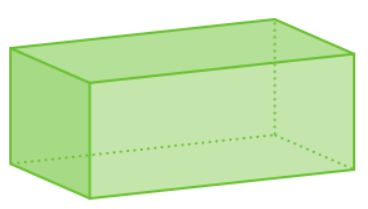
\includegraphics[width=0.4\linewidth]{chapters/chapter 5/top-ov-box.png}
\end{figure}

որի ձախ և աջ նիստերը քառակուսիներ են։ 

Ամենաշատը որքա՞ն կարող է լինել այդ տուփի ծավալը։ 

\hint{Նախ՝ մի քիչ երկրաչափություն։ Վերցրեք ոչ քառակուսի նիստերից մեկը, նշանակեք դրա երկարությունն ու լայնությունը $x$ և $y$։ Կարո՞ղ եք $y$-ն արտահայտել $x$-ով։ Իսկ ծավալը՝ $x$-ո՞վ։}
\end{problem}
\setchapterpreamble[u]{\margintoc}
\chapter{Մոտարկում և ինտեգրում}
\labch{approx_integration}

\emergencystretch 2em

\section{Թեյլորի բազմանդամ}

Սովորաբար երբ փորձում են, ասենք, վերականգնել մեքենայի կամ ինքնաթիռի շարժման հետագիծը, վերցնում են ժամանակի ինչ-որ պահի (ասենք՝ շարժումը սկսելուց $t=2$ վ անց) նրա ունեցած դիրքը, արագությունը, արագացումը, արագացման արագությունը, և այլն, ու փորձում այդ թվերի միջոցով %\marginnote{ընդ որում՝ ինչքան շատ տվյալ ունե\-նանք, այնքան ճշգրիտ կվերականգնենք}
հաշվել, թե որ կետում կգտնվի մարմինը ենթադրենք՝ $t=3$ պահին։

Նույն ձևով՝ եթե ունենք որևէ $a$ կետում ինչ-որ մի անհայտ $f$ ֆունկցիայի արժեքը, ածանցյալը, երկրորդ կարգի ածանցյալը, և այլն, ապա կարող ենք մոտավորապես վերականգնել այդ $a$ կետի մոտակայքում $f$-ի ունեցած արժեքներն ու նրա գրաֆիկը։ Ինչպե՞ս դա անենք։

\question{Որքա՞ն են $f(x) = 10 + 5(x-3)$ ֆունկցիայի արժեքն ու ածանցյալը $x=3$ կետում։}

\begin{marginfigure}
    \centering
    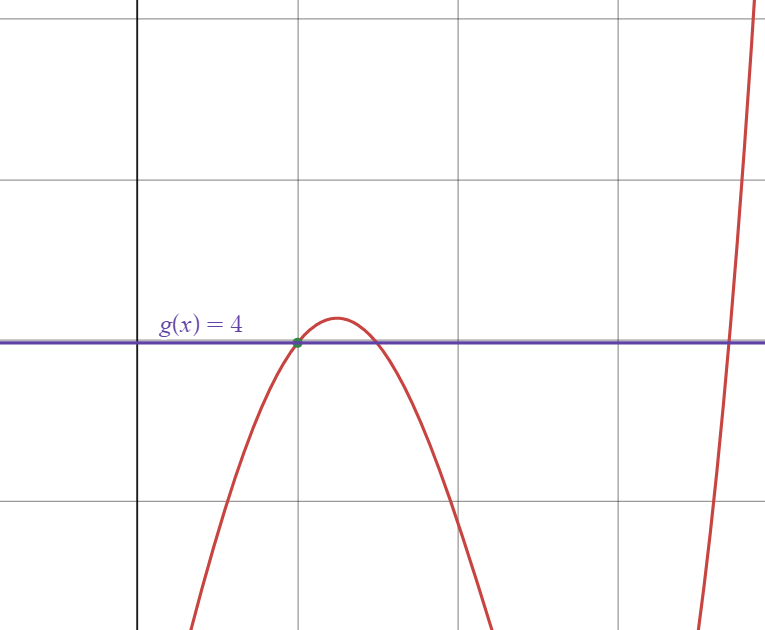
\includegraphics[width=\linewidth]{chapters/chapter 6/Taylor_1.1.png}
\end{marginfigure}

Ենթադրենք՝ ունենք, որ $f(a)=4$ և $f'(a)=3$։ Սկզբի համար կարող ենք վերցնել, ասենք, 
\[
g(x)=4  
\] 
ֆունկցիան, և այն $a$ կետում իր արժեքով հավասար կլինի $f$-ին՝ $g(a)=f(a)$։ Որպեսզի հավասարացնենք նաև $a$ կետում $f$-ի և $g$-ի ունեցած արագությունները, $g$-ին գումարենք այնպիսի բան, որի ածանցյալը $3$ է (օրինակ՝ $3x$), բայց որը գումարելով $g$-ի արժեքը չենք փչացնի (այսինքն՝ կշարունակենք ունենալ $f(a)=g(a)$)։ Գումարելով $3(x-a)$՝ կստանանք
\[
g(x)=4+3(x-a)
\]

Իրոք, եթե ստացված ֆունկցիան ածանցենք, կունենանք՝ $g'(a)=3$, ուրեմն՝ $g(a)=f(a)$ և $g'(a)=f'(a)$․ մեր սարքած $g$ ֆունկցիայի և՛ արժեքը, և՛ ածանցյալը համընկնում են $f$-ինի հետ։ Իհարկե, սա դեռ չի նշանակում, որ $f$-ն ու $g$-ն նույն ֆունկցիաներն են․ միգուցե ասենք՝ երկրորդ կարգի ածանցյալով դրանք իրարից տարբերվեն ($f''(a)\ne g''(a)$) և նույնը չլինեն։ Բայց երկրորդ կարգի ածանցյալի արժեքը (արագացումը) սովորաբար զգացվում է, երբ $a$ կետից փոքր-ինչ հեռանում ես, մինչդեռ եթե մենք շատ-շատ մոտ մնանք $a$ կետին, ապա $g$-ի արժեքները ու գրաֆիկը մոտավորապես նույնը կլինեն, ինչ $f$-ինը՝ 
\[
g(x) \approx f(x) \qquad \text{երբ $x$-ը շատ մոտ է $a$-ին}
\]

\begin{marginfigure}
    \centering
    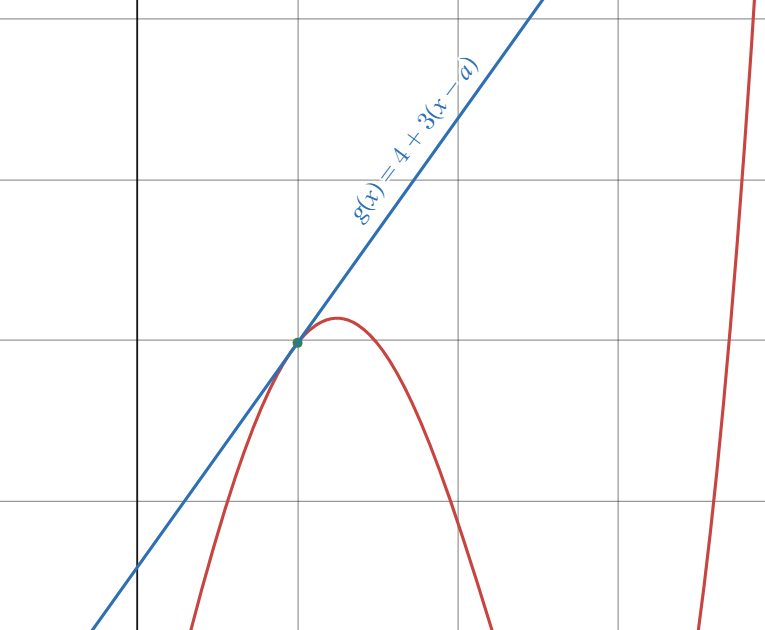
\includegraphics[width=\linewidth]{chapters/chapter 6/Taylor_1.2.png}
\end{marginfigure}

այլ կերպ ասած՝ մեր ստացած $g$ ֆունկցիան \textit{մոտարկում է} $f$-ին (թեև ոչ այնքան ճշգրիտ կերպով)։

Եթե ուզում ենք, որ այն ավելի ճշգրիտ մոտարկի, գնանք մեկ այլ առաջ․ փորձենք կառուցել այնպիսի $g$, որի արագացումը նույնպես համընկնի $f$-ինի հետ։ Ենթադրենք՝ $f''(a)=5$։

\question{Ի՞նչ գումարենք $g(x)$-ին, որպեսզի դրա երկրորդ կարգի ածանցյալը նույնպես $a$ կետում լինի $5$՝ $g''(a)=5$:}

Երկրորդ կարգի ածանցյալը ստանալու համար ավելացնենք ևս մեկ գումարելի՝
\[
g(x)=4+3(x-a)+\frac{5}{2}(x-a)^2
\]

\begin{marginfigure}
    \centering
    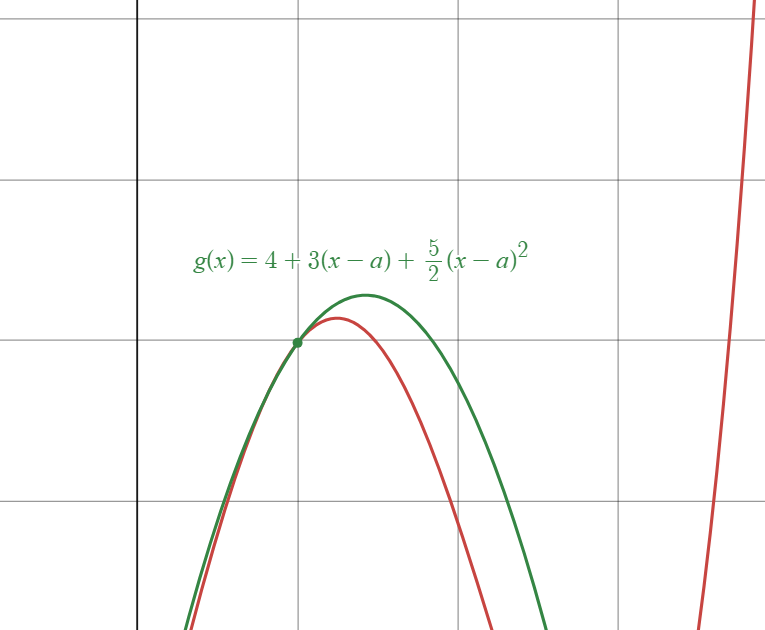
\includegraphics[width=\linewidth]{chapters/chapter 6/Taylor_1.3.png}
\end{marginfigure}

Կրկին, դժվար չէ ստուգել, որ այս ֆունկցիայի համար $g''(a)=f''(a)=5$ և $g(a)=f(a)$, $g'(a)=f'(a)$: Ինչո՞ւ ենք բազմապատկում $\dfrac{1}{2}$-ով․ որպեսզի ածանցելիս $(x-a)^2$-ու ցուցիչը իջնելով բազմապատկվի և կրճատվի դրա հետ (հակառակ դեպքում $g''(a)$-ն $2$ անգամ մեծ կլիներ)։

Այս սխեմայով եթե շարունակենք, կստանանք հետևյալ ֆունկցիան՝
\[
g(x) = f(a) + f'(a)\cdot (x-a) + \frac{f''(a)}{2}\cdot (x-a)^2 + \frac{f'''(a)}{3 \cdot 2}\cdot (x-a)^3 + \dots
\]
որը $a$ կետում կունենա
\begin{itemize}
    \item նույն արժեքը, ինչ $f$-ը
    \item նույն արագությունը, ինչ $f$-ը
    \item նույն արագացումը, ինչ $f$-ը
    \item նույն արագացման արագությունը, ինչ $f$-ը
    \item \dots 
\end{itemize}
հետևաբար բավական մոտ կլինի իսկական $f$ ֆունկցիայի արժեքներին $a$ կետի շրջակայքում։ Քանի որ գործնականում ոչ հնարավոր է, ոչ էլ կարիք կա հաշվելու բոլոր (անվերջ քանակով) ածանցյալները, սովորաբար բավարարվում են գրելով միայն առաջին մի քանի գումարելիները՝
\begin{align*}
P_k(x) &= f(a) + f'(a)\cdot (x-a) + \frac{f''(a)}{2}\cdot (x-a)^2 \\&+ \dots +
 \frac{f^{(k)}(a)}{k \cdot (k-1) \cdot \dots \cdot 2}\cdot (x-a)^k 
 = \sum_{j=1}^k \frac{f^{(j)}(a)}{j!}(x-a)^j
\end{align*}
և ստացված ֆունկցիան անվանում \textit{$k$-րդ կարգի \href{https://en.wikipedia.org/wiki/Taylor_Swift}{Թեյլորի} բազմանդամ։}

\begin{theorem}
Եթե $f(x)$ ֆունկցիան $k$ անգամ դիֆերենցելի\marginnote{$k$ անգամ դիֆերենցելի $=$ ունի $1$-ին, $2$-րդ, $\dots$, $k$-րդ կարգի ածանցյալներ} է $a$ կետում, ապա
\[
P_k(x) \approx f(x)
\]
$a$ կետի ինչ-որ (միգուցե՝ փոքր) շրջակայքում։ Ավելի \marginnote[*+2]{ի՞նչ կլինի, եթե օրինակ $x-a=0.1$, $k=5$}ճշգրիտ՝
\[
P_k(x) - f(x) = c \cdot (x-a)^{k+1}
\]
որտեղ $c$-ն ինչ-որ ֆիքսված թիվ է (արժեքը կարևոր չէ)։
\end{theorem}

\question{Կարո՞ղ եք գտնել $f(x)=x^2+7x-6$ ֆունկցիայի $10$-րդ կարգի Թեյլորի բազմանդամը։ Իսկ ո՞րն է դրա $2$-րդ կարգինը։ Իսկ $1$-ի՞ն։}

Այսինքն՝ որքան $k$-ն՝ գումարելիների թիվը, մեծացնենք, այնքան ավելի ճշգրիտ մոտարկում կստանանք $a$ կետին մոտիկ կետերում։ Համոզվելու համար \href{https://math.libretexts.org/Learning_Objects/Interactive_Calculus_Activities/Power_Series_1_Over_1-x}{տեսեք}, օրինակ, $\dfrac{1}{1-x}$ ֆունկցիայի Թեյլորի բազմանդամները։ Գործնականում հաճախ վերցնում են ընդամենը առաջին $k=1$ (գծա\-յին), $2$ (քառակուսային) կամ $3$ (խորանարդային մոտարկումներ) գումա\-րե\-լի\-ները․ մի կողմից դրանք բավարար ճշգրիտ են, մյուս կողմից՝ ավելի մեծ $k$-երի դեպքում ունենում ենք բարձր աստիճանի բազմանդամ, որը $a$-ից հեռու կետերում իրեն \marginnote{լավ չի պահում $=$ շատ է տատանվում}լավ չի պահում։

\warning{Նույն ֆունկցիայի համար, սակայն տարբեր $a$ կե\-տե\-րում գրված Թեյլորի բազմանդամները տարբերվում են։ Յուրաքանչյուրը լավ է մոտարկում միայն իր $a$ կետին մոտիկ տեղամասում, $a$-ից հեռանալիս՝ ճշգրտությունն ընկնում է։}

\begin{example}
$a=0$ կետի համար հետևյալ ֆունկցիաները կարելի է գրել՝
\begin{itemize}
\item $\displaystyle e^x = \sum_{n=0}^{\infty} \dfrac{x^n}{n!} = 1 + x + \dfrac{x^2}{2!} + \dfrac{x^3}{3!} + \cdots$

\item $\displaystyle \dfrac{1}{1-x}= \sum_{n=0}^\infty x^n = 1+x+x^2+x^3+x^4+\cdots $

\item $\displaystyle\ln(1+x)=\sum_{n=0}^\infty(-1)^n\dfrac{x^{n+1}}{n+1}=x -
\dfrac{x^2}{2} + \dfrac{x^3}{3} - \dfrac{x^4}{4}+ \cdots$

\item եթե $f$-ն ինքը բազմանդամ է, ապա $P_k$-ն նրա առաջին $k$ անդամներն են
\end{itemize} 
\end{example}

\question{Օգտվելով $\dfrac{1}{1+x}$-ի Թեյլորի բազմանդամից՝ ինչպե՞ս ստա\-նանք  $\dfrac{1}{1-x}$-ի Թեյլորի բազմանդամը։ }


\section{Անորոշ ինտեգրալ}

Ֆունկցիայի Թեյլորի բազմանդամը կառուցելիս առնչվեցինք նման հարցի․ ո՞ր ֆունկցիայի ածանցյալն է հավասար $3$-ի։ Քանի որ գիտեինք, թե ինչի են հավասար մի քանի տարբեր ֆունկցիաների ածանցյալները, հետ գնալով կռահեցինք, որ այդպիսի ֆունկցիա է $3x$-ը։

\question{Ո՞ր ֆունկցիայի ածանցյալն է $4x^3$։}

Ընդ որում $3x$-ից բացի նույն ածանցյալն ունեն նաև $3x+1$, $3x+4$, $3x-1000$ ֆունկցիաները։ Պատճառն այն է, որ երբ $3x$-ին գումարում ենք որևէ հաստատուն թիվ՝ $c$, վերջինիս ածանցյալը զրո է։ Ուրեմն $3x+c$ տեսքի բոլոր ֆունկցիաների ածանցյալները հավասար են $3$ ֆունկցիային։

Կարճ կասենք, որ եթե
\[
f\text{-ը }F\text{-ի ածանցյալն է}
\]
ապա
\[
F\text{-ը }f\text{-ի \textbf{նախնականն} է}
\]
իսկ $F$ ֆունկցիայի բոլոր նախնականները իրար հետ (բոլոր նախնա\-կան\-ների բազմությունը) կանվանենք $F$-ի \textit{անորոշ ինտեգրալ։} 

Փաստորեն ֆունկցիայի նախնականը այն ֆունկցիան է, որը պատաս\-խա\-նում է «ո՞ր ֆունկցիան ածանցեմ, որպեսզի ստանամ այս ֆունկցիան» հարցին, և բավարար է գտնել նմանատիպ որևէ ֆունկցիա ու դրան հաստատուն թվեր գումարելով՝ կստանանք մնացած բոլոր նախնական\-ները։

\begin{theorem}
$f$ ֆունկցիայի բոլոր նախնականներն իրարից տար\-բեր\-վում են հաստատուններով։
\end{theorem}

\begin{example}
$f(x)=4x^3$ ֆունկցիայի համար նախնական են
\begin{itemize}
    \item $x^4$
    \item $x^4+5$
    \item $x^4+100000000$
    \item $\dots$
\end{itemize}
ֆունկցիաները, այսինքն $f(x)$-ի բոլոր նախնականներն ունեն հետևյալ տեսքը՝ \marginnote{որտեղ $c$-ն ցանկացած հաստատուն է}
\[
x^4 + c
\]
\end{example}

$f(x)$-ի բոլոր նախնականները, նույն ինքը՝ անորոշ ինտեգրալը, կնշանակենք այսպես՝
\[
\int f(x) \, dx
\]
տվյալ օրինակում՝
\[
\int 4x^3 \, dx = x^4 + c
\]

Այս $\int$-ն ու $dx$-ը ընդամենը ինչ-որ սիմվոլներ են (ոչ մի բազմապատկում կամ այլ իմաստ չկա), որոնց արանքում գրում ենք մեր ինտեգրվող ֆունկցիան։ 

\question{Ո՞ր ֆունկցիան է և՛ ինքը իր նախնականը, և՛ ածանցյալը։}

Ինտեգրալը նույնպես օժտված է գծային հատկություններով․\marginnote[*+2]{$a$-ն ցանկացած թիվ է}
\begin{align*}
\int a \cdot f(x) \,dx &= a \cdot \int  f(x) \,dx
\\\int f(x) \pm g(x) \,dx &= \int f(x) \,dx \pm \int g(x) \,dx
\end{align*}

Եթե երկու ֆունկցիաների գումարը ինտեգրելիս դրանց որոշում ենք առանձին-առանձին ինտեգրել, յուրաքանչյուրի ինտեգրալը հաշվելիս ունենում ենք $+c$: Արդյունքում գումարի մեջ ունենում ենք $+2c$, որը սակայն կարող ենք գրել պարզապես $+c$․ այս $c$-երը կարող են լինել ցանկացած թվեր, և տարբերություն չկա՝ \marginnote{այսինքն՝ կարող ենք գրել \[\int 3x^2 + 4x \, dx = x^3 + 2x^2 + c\]} վերցնել ցանկացած թվին գումարել մեկ ուրիշ ցանկացած թիվ, թե՞ պարզապես վերցնել ինչ-որ մի երրորդ ցանկացած թիվ։

\question{Կարո՞ղ եք գտնել $\int \cos x \, dx$-ը։ Իսկ $\int 2x \cos (x^2)\, dx$-ը՞:}

Հիշենք երկու ֆունկցիաների արտադրյալի ածանցման կանոնը՝ 
\[
(fg)'=f'g+fg'
\]

Եթե մեզ պետք լիներ ստանալ ասենք՝ աջ մասի երկրորդ գումարելիի ինտեգրալը, կարող էինք նախ այն գրել այս տեսքով՝
\[
f(x)g'(x) = \underbrace{(f(x)g(x))'}_{\text{ո՞րն է նախնականը}} - f'(x)g(x)
\]
ապա երկու կողմերն ինտեգրել՝
\[
\int f(x)g'(x) \, dx = f(x)g(x) - \int f'(x)g(x) \, dx
\]

Այս բանաձևը հաճախ է օգտագործվում ինտեգրալներ հաշվելիս և կոչվում է \textit{մասերով ինտեգրում։} Հաճախ $g'(x)\,dx$-ի փոխարեն կարճ գրում են՝ $dg(x)$․
\[
\int f(x)g'(x) \, dx = \int f(x)\, dg(x)
\]
Նույն ձևով գրելով $f'(x)\, dx = df(x)$՝ կունենանք
\[
\int f\, dg = fg - \int g\, df
\]

\begin{marginfigure}
    {\centering \@setfontsize\Huge{30}{60}\[\int \]}
    \caption*{ինտեգրալը կիրառվում է նաև \href{https://youtu.be/o4-3_JoXiVU?feature=shared&t=481}{կյանքում}}
\end{marginfigure}

\begin{example}
Ո՞ր ֆունկցիայի ածանցյալն է $x\cos x$-ը։ Գրենք՝
\[
\int x \cos x\, dx 
\]
ներկայացնենք $\cos x$-ը որպես մեկ ուրիշ ֆունկցիայի ածանցյալ՝ 
\[
=
\int x (\sin x)'\, dx 
=
\int x \,d (\sin x)
=
x \sin x-\int \sin x\, dx
\]
իսկ այստեղ արդեն գիտենք, թե ով է $\sin x$-ի ինտեգրալը․
\[
=
x \sin x-\int \sin x\, dx
= 
x \sin x + \cos x + c
\]
Համոզվելու համար կարող ենք ստացվածը ածանցել և տեսնել, որ իրոք լինում է $x \cos x$: 
\end{example}

\question{Ո՞ր ֆունկցիաներն են $x^{100}$-ի նախնականները։}

Առայժմ ինտեգրելը խաղի նման ինչ-որ բան է՝ վերցնում ես ֆունկցիան, կռահում, թե ում ածանցյալն է։ Շուտով կպարզենք, թե ո՞րն է դրա կիրառական նշանակությունը։ Մինչ այդ ֆիքսենք մի քանի հայտնի ֆունկցիաների անորոշ ինտեգրալները՝
\begin{itemize}
\item $\displaystyle \int a \, dx= ax+c$
\item $\displaystyle \int x \, dx= \dfrac{x^2}{2}+c$
\item $\displaystyle \int x^n \, dx= \dfrac{x^{n+1}}{n+1}+c$ (բացառությամբ երբ $n=-1$)
\item $\displaystyle \int \dfrac{1}{x} \, dx= \int x^{-1} \, dx= \ln|x| + c$
\item $\displaystyle \int e^x \, dx= e^x+c$
\item $\displaystyle \int \cos x \, dx= \sin x+c$
\item $\displaystyle \int \sin x \, dx= $ լրացրու ինքդ
\end{itemize}

\question{Եթե ածանցյալը ֆունկցիայի արագությունն է, ապա ի՞նչ եք կարծում, ինտեգրա՞լն ինչը պիտի լինի։}

\section{Որոշյալ ինտեգրալ}

Նկարում պատկերված է մեքենայի արագության գրաֆիկը՝ կախված ժամանակից: Ինչպես հայտնի է, երբ մեքենան շարժվում է հավասարաչափ արագությամբ, նրա անցած ճանապարհը հավասար է ժամանակ $\times$ արագություն, այսինքն՝ $t \in [0, 10]$ միջակայքում մեքենայի անցած\marginnote{կարող ենք համարել՝ $v(t)=s'(t)$} ճանապարհը $= 100$ մ $=$ քառակուսի մասի մակերեսին։

\begin{figure}[h]
    \centering
    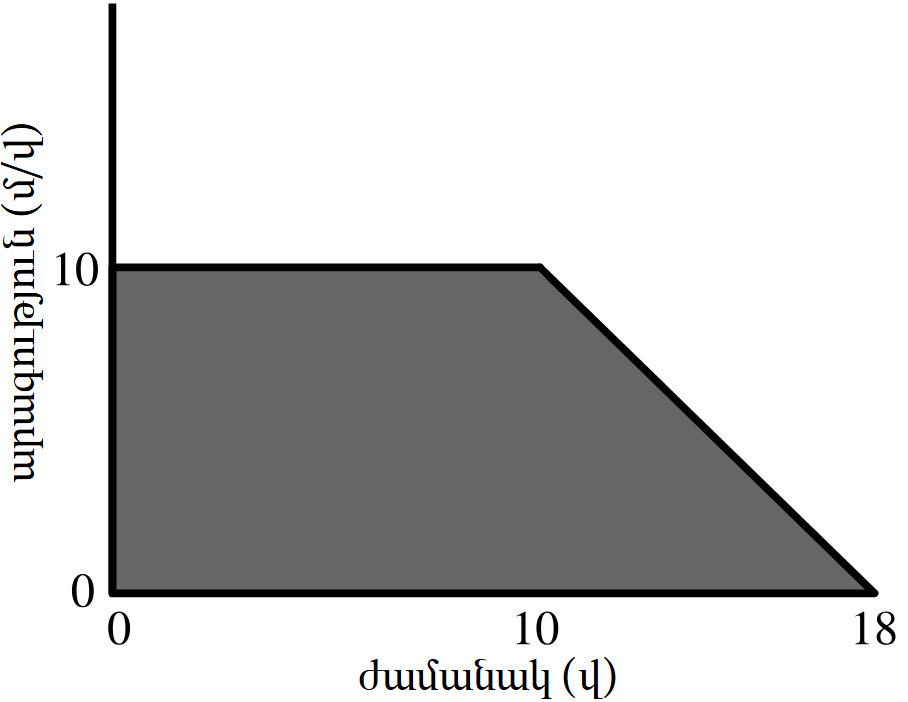
\includegraphics[width=0.6\linewidth]{chapters/chapter 6/velocity.png}
\end{figure}

$t=10$ պահից սկսած մեքենայի արագությունը սկսում է հաստատուն արագացմամբ նվազել և ի վերջո դառնում է $0$։ Ուրեմն $t \in [10, 18]$ միջակայքում մեքենայի միջին արագությունն է $5$, հետևաբար նրա անցած ճանապարհը $= 40$ մ $=$ եռանկյուն մասի մակերեսին։

Ինչպես նկատում եք, կա օրինաչափություն․ մարմնի անցած ճանապարհը յուրաքանչյուր $t\in [a, b]$ ժամանակահատվածում հավասար է $t=a$ և $t=b$ կետերի միջև նրա արագության գրաֆիկի տակ եղած մակերեսին։ Այս սկզբունքը ճիշտ է ոչ միայն հաստատուն կամ հավասարաչափ դանդաղող շարժման, այլ առհասարակ ցանկացած շարժման դեպքում։

\question{$s(t)$ ֆունկցիայի ի՞նչն է $v(t)$-ն։ Իսկ $v(t)$-ի ի՞նչն է $s(t)$-ն։}

Իսկ ի՞նչ, եթե արագության գրաֆիկը բաղկացած լիներ ոչ թե քառակու\-սուց և եռանկյունից, այլ լիներ ավելի բարդ տեսքի։ Ինչպե՞ս հաշվել այս կամ այն ֆունկցիայի գրաֆիկի տակ եղած մակերեսը։

\begin{figure}[t]
\centering %
\floatsetup{floatrowsep=qquad}
\begin{floatrow}[3]%
\ffigbox[\FBwidth]{}{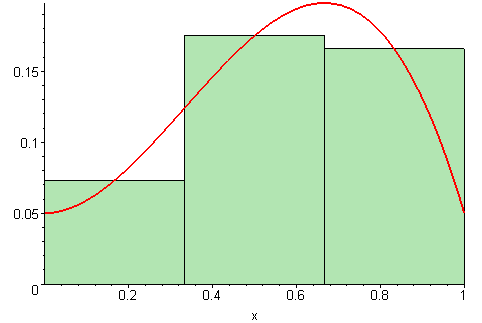
\includegraphics[width=0.4\textwidth]{chapters/chapter 6/Riemann 1.png}}
\ffigbox[\FBwidth]{}{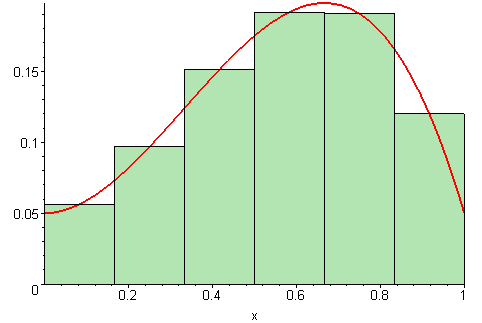
\includegraphics[width=0.4\textwidth]{chapters/chapter 6/Riemann 2.png}}
\ffigbox[\FBwidth]{}{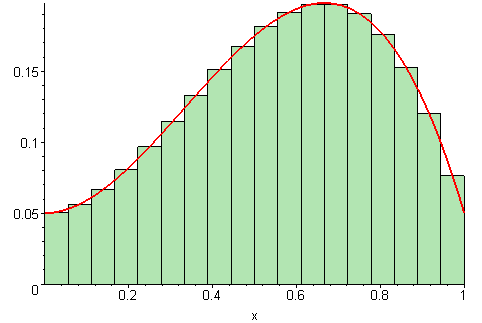
\includegraphics[width=0.4\textwidth]{chapters/chapter 6/Riemann 3.png}}
\end{floatrow}
\end{figure}

% \begin{figure}[h]
%     \centering
%     \subfloat{{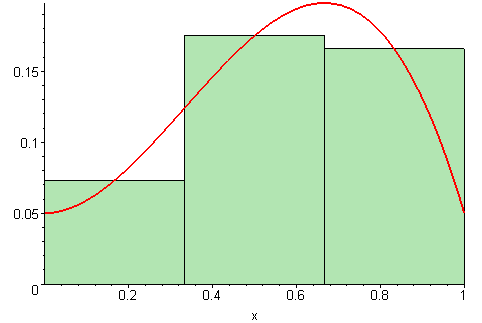
\includegraphics[width=0.3\linewidth]{chapters/chapter 6/Riemann 1.png} }}%
%     \quad
%     \subfloat{{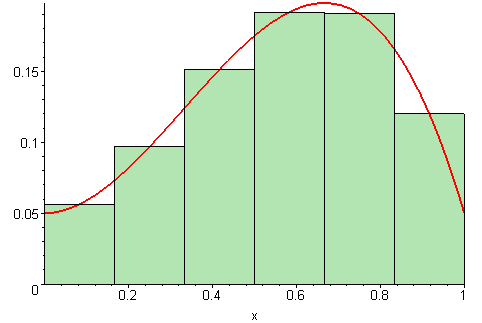
\includegraphics[width=0.3\linewidth]{chapters/chapter 6/Riemann 2.png} }}%
%     \quad
%     \subfloat{{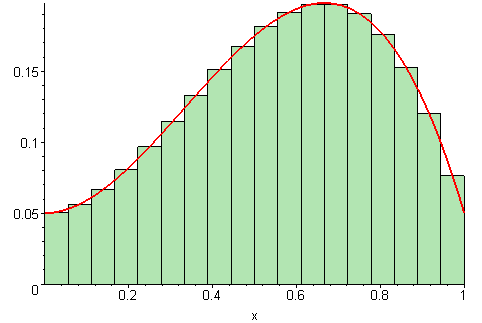
\includegraphics[width=0.3\linewidth]{chapters/chapter 6/Riemann 3.png} }}%
% \end{figure}

Ինչպես և հավանաբար կանեիք առօրյա կյանքում, մոտարկենք այդ մակերեսը \textit{ուղղանկյուններով․} բաժանենք մեր $[a, b]$ միջակայքը (տրոհենք) բազ\-մա\-թիվ փոքր հատվածիկների՝\marginnote[*+1.9]{որտեղ $x_0=a$, իսկ $x_n=b$}
\[
[x_0, x_1],\quad [x_1, x_2],\quad \dots, \quad [x_{n-1}, x_n]
\]
յուրաքանչյուր $k$-րդ հատվածի չափը նշանակելով $\Delta x_k$-ով՝ $\Delta x_k = x_{k}-x_{k-1}$, այնուհետև յուրաքանչյուր հատվածի վրա կառուցենք այնպիսի ուղղանկյուն, որը մոտիկ լինի այդ հատվածի վրա $f$-ի գրաֆիկին։ Քանի որ $f$-ի գրաֆիկի «բարձրությունը» պարզապես ամեն կետում $f$-ի ընդունած արժեքն է, ամեն $[x_{k-1}, x_k]$ հատվածում վերցնենք որևէ $c_k$ կետ և դիտարկենք այն ուղղանկյունը, որի
\begin{itemize}
    \item բարձրությունը $f(c_k)$ է
    \item հիմքը՝ $[x_{k-1}, x_k]$ հատվածը
\end{itemize}

Ստացված ուղղանկյան մակերեսը կլինի $f(c_k) \cdot \Delta x_k$, հետևաբար բոլոր ուղղանկյունների մակերեսը միասին՝
\[
\sum_{k=1}^{n} f(c_k)\, \Delta x_k
\]
Որքան $n$-ը մեծ լինի, իսկ հատվածիկների երկարությունները՝ փոքր, այնքան այս գումարը մոտ կլինի $f$-ի գրաֆիկի տակ եղածին։ Այն թիվը, \marginnote{$c_k$-երի ընտրությունը այստեղ կարևոր չէ, քանի որ վերջում \href{https://www.sfu.ca/math-coursenotes/Math\%20158\%20Course\%20Notes/sec_defint.html##:~:text=1.4.2}{նույն թիվն} ենք ստանալու (երբ $n \to \infty$)} որը կստանանք՝ վերևի գումարում հատվածների երկարությունները ձգտեցնելով $0$-ի, ցույց կտա $[a,b]$ միջակայքում $f$-ի գրաֆիկով սահ\-մա\-նա\-փակված մակերեսը և կկոչվի $f$ ֆունկցիայի \textit{որոշյալ ինտեգ\-րալ} այդ միջակայքում։

\begin{definition}
Հետևյալ թիվը՝ \marginnote{ավելի ճշգրիտ՝ ոչ թե  
$\lim\limits_{n \to \infty}$, այլ $\lim\limits_{\lambda \to 0}$, որտեղ $\lambda$-ն ամենաերկար հատվածի եր\-կա\-րու\-թյունն է
}
\[
\lim_{n \to \infty} \sum_{i=1}^n f(c_i) \,\Delta x_i
\]
կոչվում է $f(x)$ ֆունկցիայի \textbf{որոշյալ ինտեգրալ} $[a,b]$ միջակայքում և նշանակվում՝
\[
\int_a^b f(x)\, dx
\]
\end{definition}

\newpage
\begin{marginfigure}
\centering
\caption*{ասում են, որ $\int_a^b f(x)\,dx$-ը \textit{նշանափոխ} մակերես է ({\it signed} {\rm area})}
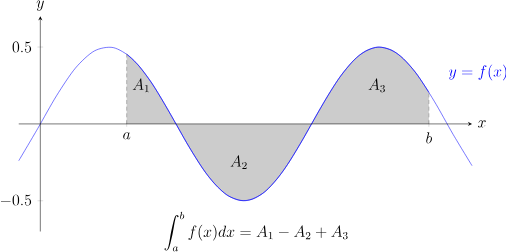
\includegraphics[width=\linewidth]{chapters/chapter 6/net area.png}
\end{marginfigure}Այստեղ անենք մի կարևոր նշում։ Եթե $f(x)$-ի արժեքները $[a,b]$ միջակայքում դրական են, այսինքն՝ նրա գրաֆիկը ընկած է $x$-երի առանցքից վերև, ապա $\int_a^b f(x)\,dx$-ը իրոք կտա դրանից ներքև եղած մակերեսը, բայց եթե այն բացասական է՝ $f(x) < 0$ ($x$-երի առանցքից ներքև), ապա $\int_a^b f(x)\,dx$-ի արժեքը կլինի \textit{բացասական՝} $f$-ի գրաֆիկի և $x$-երի առանցքի արանքում ընկած մակերեսը, սակայն մինուս նշանով։ Այսինքն կախված $[a,b]$-ում $f$-ի նշանից՝ դրա որոշյալ ինտեգրալը մոդուլով հավասար է նրա գրաֆիկով սահմանափակված մակերեսին, իսկ նշանով համընկնում է $f$-ի հետ։

\question{Որքա՞ն է $\int_a^b f(x)\,dx$-ը, եթե $f$-ը $[a,b]$ միջակայքում հավասար է $0$-ի։ Հնարավո՞ր է, որ $\int_a^b f(x)\,dx=0$, բայց $f$-ը $0$ չլինի։}

\section{Նյուտոն-Լայբնիցի բանաձևը}

Ինչպե՞ս հաշվել $\int_a^b f(x)\,dx$-ը, եթե ունենք $f(x)$-ի բանաձևը (կամ առհասարակ ինչո՞ւ է այն կոչվում «ինտեգրալ»)։ Օրինակ՝ երբ $f$-ը մարմնի արագությունն է, որը իր հերթին անցած ճանապարհի ածանցյալն է՝ ${f(t) = v(t) = s'(t)}$, ապա ${t=a}$ և ${t=b}$ կետերի միջև նրա գրաֆիկի տակ եղած մակերեսը այդ ընթացքում մարմնի անցած ճանապարհն է՝ $\int_a^b v(t)\, dt=s(b)-s(a)$։ Պարզվում է, որ այս կանոնը ճիշտ է ցանկացած դեպքում․

\begin{theorem}
Եթե $F(x)$ ֆունկցիան $f(x)$-ի որևէ նախնական է, ապա
\[
\int_a^b f(x)\,dx = F(b)-F(a)
\]
\end{theorem}

Այսինքն՝ ֆունկցիայի տակ եղած մակերեսը երկու կետերի միջև հավասար է այդ կետերի միջև իր նախնականի \textit{փոփոխությանը։} Ճիշտ է՝ $f$-ը ունի ոչ թե մեկ նախնական, այլ անվերջ հատ, \marginnote{եթե $G$-ն նույնպես $f$-ի նախնական է, ապա $G(x) = F(x) + c$, հետևաբար $$G(b)-G(a)=F(b)-F(a)$$} բայց դրանց բոլորի տարբերությունները երկու կետերի միջև նույնն են։ Ուրեմն՝ $\int_a^b f(x)\,dx$-ը հաշվելու համար հաշվում ենք (անորոշ) $\int f(x)\,dx$-ը, այսինքն՝ գտնում $f$-ի որևէ $F$ նախնական (տարբերություն չկա, թե որը), և հաշվում դրա արժեքների տարբերությունը $a$ և $b$ կետերում։

\begin{example}
\marginnote[*+1.5]{$F(b)-F(a)$ կարճ գրում ենք՝ $F(x)\big\vert_{x=a}^b$}$y=x^2$ պարաբոլի տակ եղած մակերեսը $x\in[0,2]$ միջա\-կայքում՝
\[
\left.\int_{0}^{2} x^2 \,dx = \frac{1}{3} \cdot  x^3\right|_{x=0}^{2} = \frac{1}{3} (2^3 - 0^3) = \frac{8}{3}
\]

Նույն կերպ $y=\sin x$-ինը $x\in [0, \pi]$-ում՝
\[
\left.\int_{0}^{\pi} \sin x \,dx =  -\cos x\right|_{x=0}^{\pi} = -\cos \pi - (-\cos0) = 2
\]

Նկատենք, որ $[0, \pi]$ միջակայքում սինուսը դրական է, այսինքն այն, ինչ ստացել ենք, հենց գրաֆիկի ներքևում եղած մակերեսն է։ Իսկ այ օրինակ՝ 
\[
\left.\int_{0}^{\pi} \cos x \,dx =  \sin x\right|_{x=0}^{\pi} = \sin \pi - \sin 0 = 0
\]
ոչ թե որովհետև կոսինուսի գրաֆիկի տակ մակերես չկա, այլ որով\-հետև $[0, \pi]$ միջակայքի առաջին կեսում ֆունկցիան դրական է, երկ\-րոր\-դում՝ բացասական, դրա հաշվին գումարը զրոյանում է։
\end{example}

\question{Ինչպե՞ս կհաշվեք $|\cos x|$-ի տակ եղած մակերեսը $[0, \pi]$-ում։}

Բնականաբար, որոշյալ ինտեգրալը նույնպես ունի այն գծային հատկություններն, ինչ անորոշը․
\begin{align*}
\int_{a}^{b} c \cdot f(x) \,dx &= c \cdot \int_{a}^{b} f(x) \,dx    
\\
\int_{a}^{b} f(x) \pm g(x) \,dx &= \int_{a}^{b} f(x) \,dx \pm \int_{a}^{b} g(x) \,dx
\end{align*}

Մյուս կողմից՝ ցանկացած $[a,b]$ միջակայքում եղած մակերեսը կարող ենք գրել որպես երկու մակերեսների գումար՝ $a$-ից $c$ և $c$-ից $b$․
\[
\int_{a}^{b} f(x) \,dx = \int_{a}^{c} f(x) \,dx + \int_{c}^{b} f(x) \,dx
\]

Կարող ենք նաև ավելի հեռուն գնալ և սահմանել ասենք՝ $\int_5^2 f(x)\,dx$, որպես $[2, 5]$ միջակայքում $f$-ի գրաֆիկով սահմանափակված մակերեսը՝ հակառակ նշանով․
\[
\int_{a}^{b} f(x) \,dx = -\int_{b}^{a} f(x) \,dx 
\]
և գրել նաև՝ $\int_{a}^{a} f(x) \,dx = 0$:

Վերջապես նկատենք մի այսպիսի նրբություն․ երբ գրում ենք $\int_a^b f(x)\, dx$, նկատի ունենք $f$ ֆունկցիայի գրաֆիկի տակի մակերեսը (համապատաս\-խան նշանով)։ Այդ մակերեսի արժեքի մեջ $x$ փոփոխականը որևէ դեր չի խաղում․ կարող էինք $x$-ի փոխարեն գրել, ասենք, $y$ կամ $z$՝
\[
    \int_4^{25} \sin x \, dx
    =
    \int_4^{25} \sin y \, dy
\] 
\begin{marginfigure}
\centering
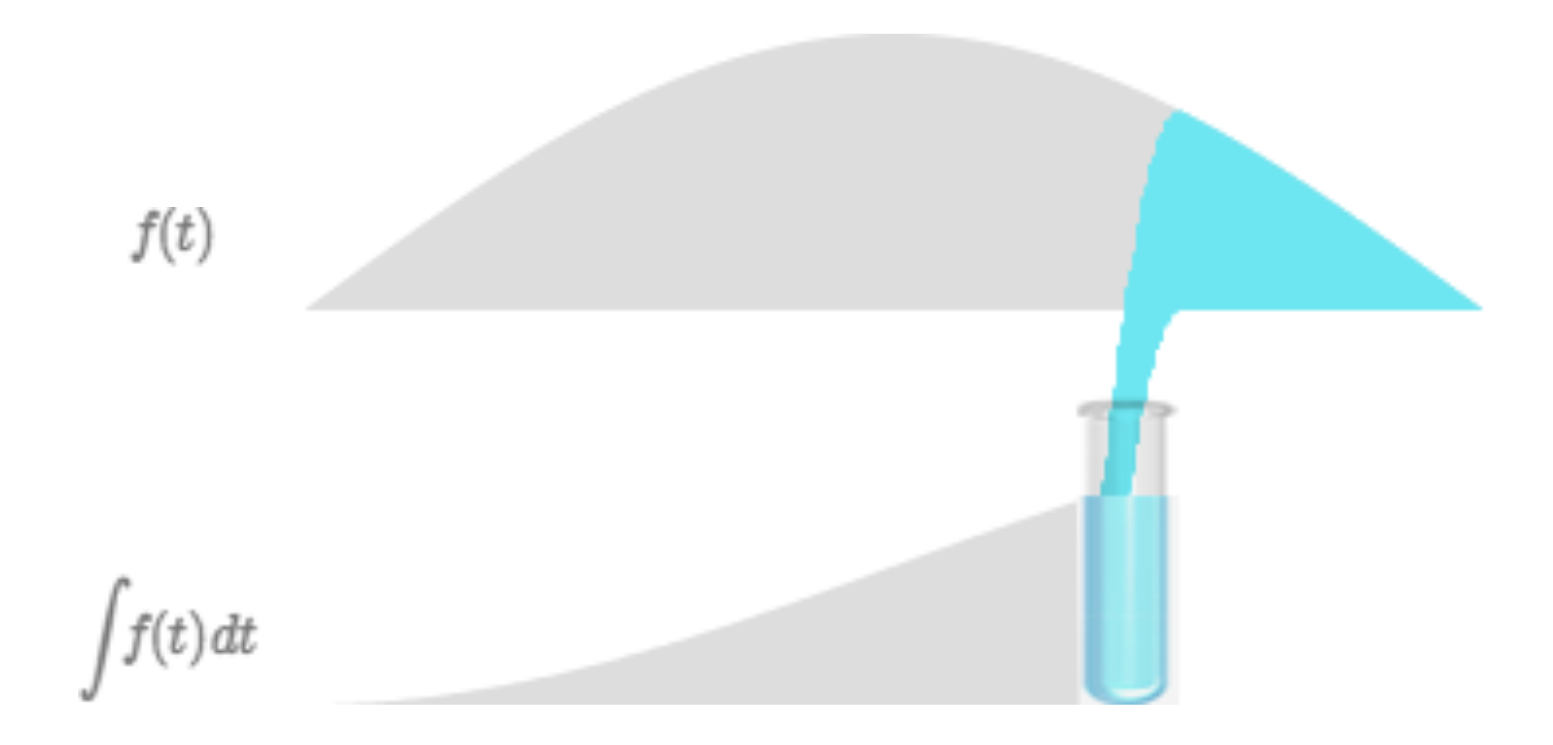
\includegraphics[width=\linewidth]{chapters/chapter 6/water filling.png}
\caption*{կամ՝ $t$-ն/$x$-ը/$y$-ը մեր բաժակն է, որը $a$-ից $b$ տանելով \href{https://worrydream.com/KillMath/#:~:text=little\%20tank\%20filling\%20up}{լցնում ենք} ջրով}
\end{marginfigure}
Պատկերավոր ասած՝ գծում ենք ֆունկցիայի գրաֆիկն ու ${y=4}$ կետից շարժվում դեպի ${y=25}$ կետը։ Ամեն կետում չափում ենք գրաֆիկի բարձրությունը, և որքան մեծ է ֆունկցիայի արժեքը, այնքան ավելի շատ մակերես ենք ստանում, որքան փոքր է՝ այնքան քիչ, իսկ բացա\-սա\-կան արժեքների դեպքում ստանում ենք բացասական մակերես։ Այս գործողության ընթացքում $y$-ը մեր պուլտն է, որով կառավարում ենք $4$-ից դեպի $25$ շարժը․ անկախ նրանից, թե ինչպես կանվանենք այդ պուլտը, ստացվող մակերեսը նույնն է։ Հետևաբար՝ ինտեգրելիս փոփոխականի անունը \textit{կարևոր չէ։}

Ավելին, կարող էինք նույնիսկ $y$-ի քառակուսի արմատը նշանակել $\sqrt{y}=t$-ով և $y$-ի փոխարեն գրել $t^2$՝ $\sin(t^2)\,d(t^2)$։ Միակ բանը, որին պետք է ուշադրություն դարձնենք, այն է, որ եթե $y$-ը փոխվում է $4$-ից $25$, ապա նրա արմատը՝ $t$-ն, պետք է փոխվի $\sqrt{4}$-ից $\sqrt{25}$, այսինքն՝
\[
\int_4^{25} \sin y \, dy = \int_2^5 \sin (t^2) \, d(t^2)
\]

\begin{example}
Հաշվենք $\dfrac{1}{x-4}$-ի գրաֆիկի տակ եղած մակերեսը $[5, 10]$ միջակայքում․
\[
\int_5^{10} \frac{1}{x-4}\, dx
\]

Ինչքան լավ կլիներ, եթե $x-4$-ի փոխարեն ունենայինք $x$։\marginnote{\hyperref[derivatives_list]{\color{OliveGreen}հիշենք}, որ $\dfrac{1}{x}$-ի նախնականը $\ln x$ է} Բայց այ եթե $x-4$-ը նշանակենք $y$-ով, կունենանք հենց $\dfrac{1}{y}$։ 

Եթե $x\in [5, 10]$, ապա $y\in [5-4, 10-4]$, այսինքն՝ $y\in [1, 6]$, և կունենանք՝
\[
\int_5^{10} \frac{1}{x-4}\, dx
=
\int_1^6 \frac{1}{y}\, d(y+4)
\]
Այստեղ \marginnote{ինչպես հիշում ենք, $dg(x) = g'(x)\,dx$} $d(y+4) = (y+4)' \, dy = 1 \cdot dy$, հետևաբար՝
\[
\int_1^6 \frac{1}{y}\, d(y+4)
=
\left.\int_1^6 \frac{1}{y}\, dy
= 
\ln y
\right|_{y=1}^6 
= 
\ln 6 - \ln 1 = \ln 6 \approx 1.79
\]
\end{example}

Այս մեթոդը կոչվում է \textit{փոփոխականի փոխարինում։}

\question{Ենթադրենք $f(x)$-ի գրաֆիկը համաչափ է սկզբնակետի նկատ\-մամբ, այսինքն՝ $f(-x)=-f(x)$։ Փորձեք պատկերել այդպիսի որևէ ֆունկցիայի գրաֆիկ։ Որքա՞ն է $\int_{-10}^{10} f(x)\, dx$-ը։}


\section{Ուռուցիկություն}

Եթե $1$-ին կարգի ածանցյալը ցույց է տալիս ֆունկցիայի արագությունը, ապա $2$-րդ կարգինը ցույց է տալիս նրա արագացումը։ Փորձենք երկրա\-չափորեն մեկնաբանել դա։

Նախ՝ ենթադրենք $f'(a)>0$, ուրեմն՝ $f$-ը $a$ կետում աճում է։ \marginnote[*+4]{ի՞նչ եք կարծում, ո՞ր գրաֆիկում է ֆունկ\-ցիայի արագացումը դրական}Բայց ֆունկցիան կարող է աճել տարբեր ձևերով, ասենք այսպես՝\newline
\begin{figure}[h]
    \centering
    $\vcenter{\hbox{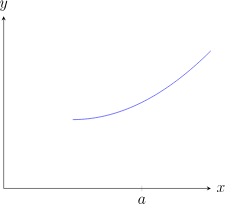
\includegraphics[width=0.3\linewidth]{chapters/chapter 6/convex.png}}}$%
    \hfill 
    կամ էլ այսպես՝
    \hfill
    $\vcenter{\hbox{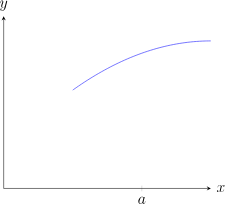
\includegraphics[width=0.3\linewidth]{chapters/chapter 6/concave.png}}}$
\end{figure}

պատկերավոր ասած՝ տակով կամ վրայով։ 

\begin{definition}
Եթե $(a,b)$ միջակայքի ցանկացած երկու կետերում ֆունկցիայի գրաֆիկն ընկած է այդ կետերը միացնող \marginnote{անգլերեն՝ ուռուցիկ — {\rm convex},\\ գոգավոր — {\rm concave}} հատվածից
\begin{itemize}
    \item ներքև, ապա կասենք, որ ֆունկցիան \textbf{ուռուցիկ} է $(a,b)$-ում
    \item վերև, ապա կասենք, որ ֆունկցիան \textbf{գոգավոր} է $(a,b)$-ում
\end{itemize}
\end{definition}

\begin{figure}[h]
    \centering
    
\includegraphics[width=0.8\linewidth]{chapters/chapter 6/convexity.png}
\end{figure}

Կետերը միացնող հատվածից վերև կամ ներքև գտնվելը կարող ենք ձևակերպել նաև այսպես․ ֆունկցիան\marginnote[*+3]{ի՞նչ է սա նշանակում $\alpha=0.5$ դեպքում}
\begin{itemize}
\item ուռուցիկ է, եթե
\[
f(\textcolor{myred}{\alpha } p + (\textcolor{myblue}{1-\alpha })q) \leq \textcolor{myred}{\alpha } f(p) + (\textcolor{myblue}{1-\alpha }) f(q)
\] 
\item գոգավոր է, եթե
\[
f(\textcolor{myred}{\alpha } p + (\textcolor{myblue}{1-\alpha })q) \ge \textcolor{myred}{\alpha } f(p) + (\textcolor{myblue}{1-\alpha }) f(q)
\]
\end{itemize}
ցանկացած $p, q \in [a,b]$ կետերի և $0 \le \alpha \le 1$ թվի դեպքում։

\warning{Ֆունկցիան կարող է մի կետում ուռուցիկ լինել, մյուսում՝ գոգավոր։}

Վերևում գրվածը չենք ապացուցի, բայց կզգանք, թե այն ինչ է նշա\-նա\-կում՝ \href{https://www.desmos.com/calculator/hx6weawigr}{բզբզալով} $\alpha$-ի արժեքները։ Ինչպես կռահում եք, ֆունկցիայի ուռուցիկ/գոգավոր լինելը կարելի է պարզել նրա երկրորդ կարգի ածանցյալի միջոցով․

\begin{theorem}
Եթե $f(x)$ ֆունկցիան երկու անգամ դիֆերենցելի է, ապա
\begin{itemize}
    \item $f$-ը ուռուցիկ է այն կետերում, որտեղ $f''(x) \ge 0$
    \item $f$-ը գոգավոր է այն կետերում, որտեղ $f''(x) \le 0$
\end{itemize}
\end{theorem}

\begin{example}
\\~
\begin{itemize}
\item $f(x) = x^2$-ն ուռուցիկ է բոլոր կետերում, քանի որ
\[
f''(x) = 2 > 0
\]
\item $f(x) = -x^2$-ն գոգավոր է բոլոր կետերում, քանի որ
\[
f''(x) = -2< 0
\]
\newpage
\item $f(x) = \sin x$-ը $(0, \pi)$ միջակայքում գոգավոր է, իսկ $(\pi, 2\pi)$-ում՝ ուռուցիկ․
\[
f''(x) = (\cos x)' = -\sin x
\]
\end{itemize}
\end{example}


\question{Ո՞ր ֆունկցիան է, որ ցանկացած կետում և՛ ուռուցիկ է, և՛ գոգավոր։}



\bigskip 

\begin{theory}
.
\begin{itemize}
\item կարդալ [{\rm Stewart}], 290-295 էջերը (ուռուցիկություն)
\item ըստ ցանկության՝ նաև [{\rm Stewart}], 325-328 էջերը
\item կարդալ [{\rm Banner}], 519-523 էջերը (Թեյլորի բազմանդամ)
\item վերադառնալ [{\rm Stewart}], 365-366, 372-373, 379-381, 391-394, 397-398 էջերին (ինտեգրալ)
\item ծանոթանալ [{\rm Stewart}]-ի 7-րդ գլխին (ինտեգրման մեթոդներ)
\item դիտել  {\rm 3b1b}-ի \href{https://www.3blue1brown.com/lessons/integration}{11-րդ} և \href{https://www.3blue1brown.com/lessons/taylor-series}{14-րդ} տեսադասերը մաթանալիզից 
\item ըստ ցանկության՝ նաև \href{https://www.3blue1brown.com/lessons/taylor-series-geometric-view}{15-րդը}
\item կարելի է նաև գտնել լուծված վարժություններ \href{https://tutorial.math.lamar.edu/Classes/CalcI/CalcI.aspx}{այստեղ}
\end{itemize}
\end{theory}

\newpage

\section{Խնդիրներ}


\begin{problem}
Գտեք $\displaystyle \int f(x)\, dx$-ը․
\begin{enumerate}[label={\alph*}․]
\item $f(x)=3x^2$
\item $f(x)=x+6\cos x$
\item $f(x)=\dfrac{3}{x}-1$
\item $f(x)=\dfrac{4x}{1-2x^2}$
\item $f(x)=\operatorname{tg}x$
\end{enumerate}
\end{problem}


\begin{problem}\marginnote[*+0.5]{\href{https://youtu.be/avDg6SmyMoY}{լուծում}}
Տիեզերանավը թռչում է Երկրից Լուսին։ Թռիչքի մեկնարկից $x$ ժամ անց նրա արագությունը
 \[f(x) = x^5+x^2\] 
հզր կմ/ժ է։
\begin{enumerate}[label={\alph*}․]
\item որքա՞ն ճանապարհ է այն անցնում առաջին $3$ ժամում
\item հետևաբար, որքա՞ն է տիեզերանավի միջին արագությունը
\end{enumerate}
\end{problem}


\begin{problem}\marginnote[*+0.5]{\href{https://youtu.be/EWhCu2C-d0M}{լուծում}}
Նկարում պատկերված է 
\[
f(x) = -x \cdot \ln (x^2)
\]
ֆունկցիայի գրաֆիկը $[0,1]$ հատվածի վրա։
\begin{figure}[h]
\centering
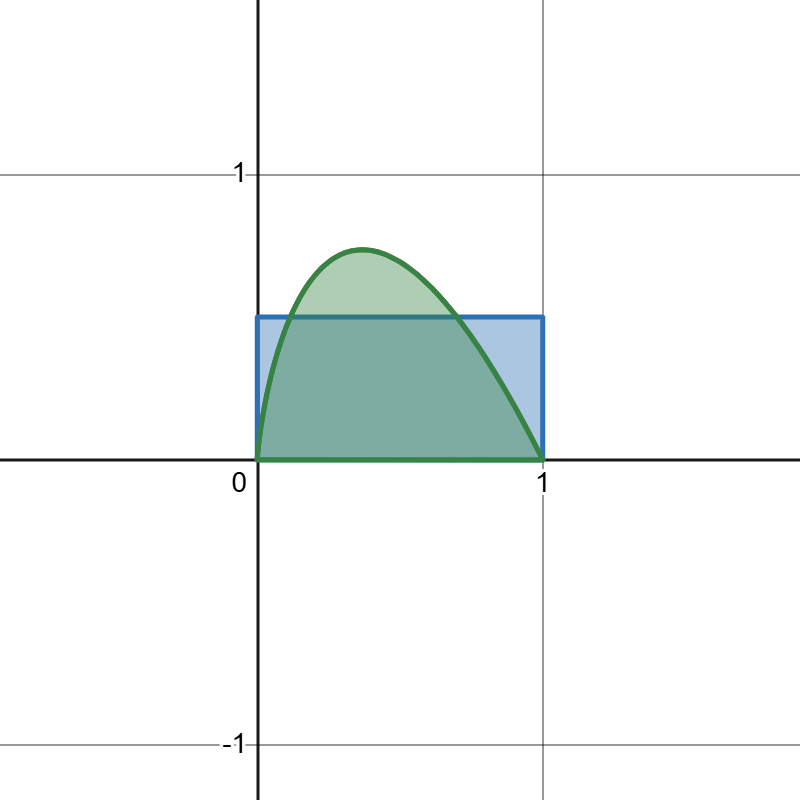
\includegraphics[trim={3cm 6cm 0 1cm},clip, width=0.5\linewidth]{chapters/chapter 6/equal_areas.png}
\end{figure}
Հայտնի է, որ կանաչ և կապույտ տիրույթներն ունեն նույն մակերեսը։
Որքա՞ն է կապույտ ուղղանկյան բարձ\-րությունը։
\end{problem}


\begin{problem}
Կան երկու ֆունկցիայից նոր ֆունկցիա ստանալու մի քանի տարբեր ձևեր։ Դրանցից մեկը, որ կարևոր դեր է խաղում մեքենայական ուսուցման մեջ, կոչվում է \textit{փաթույթ։}\marginnote[*+0.2]{անգլերեն՝ {\it convolution}}

Երկու $f$ և $g$ ֆունկցիաների փաթույթ է կոչվում (և $f*g$-ով նշանակվում) այն ֆունկցիան, որը որոշվում է հետևյալ բանաձևով՝\marginnote[*+2.4]{$x$-ը ֆիքսված է, $y$-ը փոփոխվում է}
\[
(f*g)(x) = \int_{-1}^1 f(y)g(x-y) \, dy
\]

Որքա՞ն է $f*g$-ի արժեքը $x=0$ կետում, եթե $f(x)=x^2$ և 
\[
g(x) = \begin{cases}
    1 & \text{եթե } x > 0 \\
    0 & \text{եթե } x \le 0
\end{cases}
\]

\hint{$f*g$-ում տեղադրեք $g$-ի բանաձևը, ապա բաժանեք $[-1, 1]$ միջակայքը երկու մասի՝ որտեղ որ $g=0$, և որտեղ $g=1$։}
\end{problem}


\begin{problem}
Պարզենք, թե որքան է $r$ շառավղով շրջանի մակերեսի բանաձևը։ Սկսենք $1$ շառավղով շրջանից՝ $x^2+y^2=1$։
\begin{enumerate}[label={\alph*}․]
\item արտահայտեք $y$-ն $x$-ով, ո՞ր միջակայքում է փոխվում $x$-ը
\item ո՞ր $f(x)$ ֆունկցիայի ինտեգրալն է պետք հաշվել
\item կատարեք փոփոխականի փոխարինում՝ $x$-ը նշանակելով $\sin t$-ով, ո՞ր միջակայքում պետք է փոփոխենք $t$-ն
\item ի՞նչ արտահայտություն է ստացվում ինտեգրալի նշանի տակ
\item օգտվելով $(\cos t)^2=\dfrac{1+\cos(2t)}{2}$ բանաձևից՝ հաշվեք ինտեգրալը
\item որքա՞ն է $1$ շառավղով շրջանի մակերեսը
\item ի՞նչ գծային ձևափոխություն կիրառենք՝ $r$ շառավղով շրջան ստանալու համար
\item քանի՞ անգամ կմեծանա մակերեսը
\end{enumerate}
\end{problem}

\setchapterpreamble[u]{\margintoc}
\chapter{Շատ փոփոխականի ֆունկցիա}
\labch{multi_var}

\emergencystretch 2em

\section{$f(x, y)$-ի գրաֆիկը}\label{3d_graph}

Համարենք, որ ծիրանի գործն ավարտեցինք, և վերադառնանք մեկից ավելի ապրանքների դեպքին, երբ ունենք ֆունկցիա՝ կախված մի քանի փոփոխականներից՝
\[
f(x,y) = x^{2}+y^{2}+e^{y-x}
\]

Ինչպե՞ս այս դեպքի համար ևս մշակենք գործիքներ, որոնցով կկարողա\-նանք գտնել $x$-ի ու $y$-ի այն արժեքները, որոնցում ֆունկցիայի արժեքն ամենամեծը/ամենափոքրն է։ 

Սկսենք ֆունկցիան պատկերելուց։ Նախ՝ փոփոխականը ոչ թե մեկն է, այլ երկուսը․ յուրաքանչյուր $(x, y)$ զույգի համապատասխանում է մեկ արժեք։ Հետևաբար ֆունկցիան պատկերելու համար անհրաժեշտ է
\begin{itemize}
    \item $xy$-հարթությունը՝ արգումենտների համար\marginnote[*+1]{կանվանենք՝ $z$-երի առանցք}
    \item ավելացրած մի նոր առանցք՝ արժեքները նշելու համար
\end{itemize}

\begin{figure}[h]
    \centering
    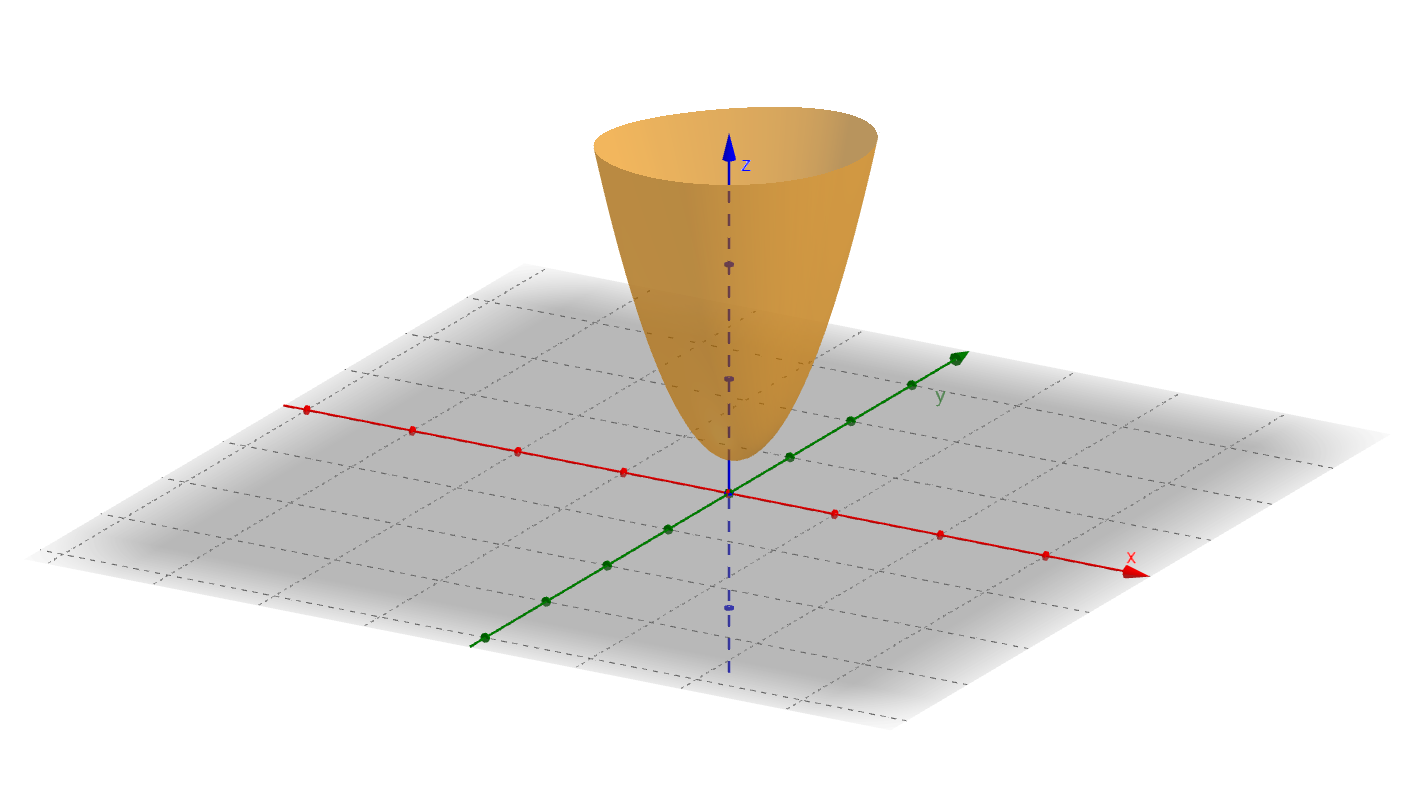
\includegraphics[width=0.75\linewidth]{chapters/chapter 7/graphing step3.png}
\end{figure}

Այժմ $xy$-հարթության ամեն մի $(x,y)$ կետի վրա բարձրանալով/իջնելով այնքան, որքան այդ կետում $f$-ի արժեքն է, կստանանք մի մակերևույթ, որը կլինի $f(x,y)$-ի գրաֆիկը։ Որպես կանոն այն նման է օդում փռված սփռոցի կամ թաշկինակի։ 

Նկատենք, որ ի տարբերություն մեկ փոփոխականի դեպքի՝ այստեղ ունենք
\begin{itemize}
   \item մեկի փոխարեն երկու առանցք
   \item երկու ուղղության փոխարեն\marginnote{հարթության մեջ ձախ/աջ չկա} անվերջ թվով ուղղություններ 
   \item հետևաբար նաև \textit{չկա աճել/նվազելու գաղափար} 
\end{itemize}
Մնացածը, կարելի է ասել, նույնն է, ինչ միաչափ դեպքում։

Լավ է մեկ անգամ տեսնել, քան հարյուր անգամ լսել․ լավ հասկանալու համար պետք է նայել \href{https://www.khanacademy.org/math/multivariable-calculus/thinking-about-multivariable-function/ways-to-represent-multivariable-functions/a/multidimensional-graphs}{տարբեր ֆունկցիաների} գրաֆիկներ։\marginnote{էլ ո՞ւր առանց \href{https://www.desmos.com/3d}{\rm Desmos}-ի ու \href{https://www.geogebra.org/3d}{\rm GeoGebra}-ի} Դե իսկ \href{https://www.intmath.com/vectors/3d-grapher.php}{երկու անգամը՝} պարզապես սքանչելի է։

Նշենք, որ երկուսից ավել փոփոխականների դեպքում գրաֆիկը դժվար է պատկերացնել, դրա համար օգտագործում են տարբեր մեթոդ\-ներ (ասենք՝ երրորդ փոփոխականի արժեքից կախված փոփոխում կետի չափսը կամ գույնը, ավելացնում անիմացիա կամ \href{https://en.wikipedia.org/wiki/Chernoff_face}{ժպիտ}): Մենք կբավարարվենք գծելով $f(x,y)$ տեսքի ֆունկցիայի գրաֆիկներ։


\section{Մասնակի ածանցյալ}

Վերադառնանք նախորդ էջում սահմանած $f(x, y)$
\hyperref[3d_graph]{\color{OliveGreen}ֆունկցիային}, որում $x$-ն ու $y$-ը խնձորի և դեղձի գներն են, իսկ ֆունկցիայի արժեքը՝ մեր եկամուտը։ 

\question{Ինչպե՞ս կչափեք, թե խնձորի արժեքը մի փոքր բարձրացնե\-լիս որքան է փոխվում եկամուտը։}

Կամ որ նույնն է՝ ինչպե՞ս հաշվենք $f(x,y)$-ի փոփոխությունը $x$-ը փոխելիս։ Դեղձի գինը՝ $y$-ը պահենք ֆիքսված, և $x$-ին փոքրիկ աճ տալով՝ շարունակենք ինչպես սովորական ֆունկցիայի ածանցյալի դեպքում․
\[
\lim_{h \to 0} \frac{f(x + h, y) - f(x, y)}{h}
\]
\marginnote{եթե $f$-ը մեկ փոփոխականի է՝ $\dfrac{df}{dx}$\\ եթե մի քանի փոփոխականի է՝ $\dfrac{\partial f}{\partial x}$}Ահա այս թիվը կանվանենք $f$-ի \textit{մասնակի ածանցյալ} ըստ $x$-ի և կնշանակենք $f_x$ կամ $\partial_x f$ կամ էլ՝ $\dfrac{\partial f}{\partial x}$։

\begin{definition}
Եթե հետևյալ սահմանը գոյություն ունի և անվերջ չէ՝
\[
f_x = \lim_{{h \to 0}} \frac{f(x + h, y) - f(x, y)}{h}
\]
ապա այն կանվանենք $f$ ֆունկցիայի \textbf{մասնակի ածանցյալ} ըստ $x$-ի։ Նույն կերպ սահմանում ենք նաև $f$-ի մասնակի ածանցյալն ըստ $y$-ի՝
\[
f_y = \lim_{{h \to 0}} \frac{f(x,y + h) - f(x, y)}{h}
\]
\end{definition}

$f_x$-ը ցույց է տալիս $f$-ի փոփոխման արագությունը միմիայն $x$-ը փոխելիս, այսինքն՝ երբ շարժվում ենք միայն $x$-երի ուղղությամբ, իսկ $y$-ին ձեռք չենք տալիս՝ պահում ենք հաստատուն։ Նույն ձևով, բնականաբար, $f_y$ = $f$-ի արագությունը $y$-ը փոխելիս՝ $x$-ը թողնելով անշարժ։

\begin{example}
Եթե $f(x, y) = x^2 + y^2$, ապա $f_x$-ը հաշվելիս համարում ենք, որ $y$-ը հաստատուն թիվ է՝
\[
f_x= (x^2)' + (y^2)' = 2x + 0 = 2x
\]
իսկ $f_y$-ը հաշվելիս՝ համարում ենք, որ $x$-ն է հաստատուն․
\[
f_y = (x^2)' + (y^2)' = 0 + 2y = 2y
\]
\end{example}

Նկատենք, որ ինչպես սովորական ֆունկցիայի ածանցյալի դեպքում, $f_x(x,y)$-ն ու $f_y(x,y)$-ը $x$-ից և $y$-ից կախված ֆունկցիաներ են և տարբեր կետերում ընդունում են տարբեր արժեքներ։

\begin{example}
Եթե $g(x, y) = 4x^{100}y$, ապա կրկին, նախ կհամարենք $y$-ը հաստատուն.\marginnote{$(\text{հաստատուն} \cdot f)' = \text{հաստատուն} \cdot f'$}
\[
f_x = 400x^{99}y
\]
հետո՝ $x$-ը․
\[
f_y = 4x^{100}
\]
\end{example}

Փաստորեն երկու փոփոխականի դեպքում ունենք ոչ թե մեկ, այլ երկու արագություն։ Եկեք այդ երկու մասնակի արագությունները խմբավորենք և գրենք մեկ վեկտորով՝
\[
\begin{bmatrix}
f_x \\ f_y
\end{bmatrix}
\]

Ստացված վեկտորը կոչվում է $f$ ֆունկցիայի \textbf{գրադիենտ} և նշանակվում է՝ $\nabla f(x,y)$։ Այն երկու ($x$-երի և $y$-ների ուղղությամբ) արագություններից կազմված վեկտորն է, և մասնավորապես վերևի օրինակում՝
\[
\nabla f(x, y) = \begin{bmatrix}
    400x^{99}y \\ 4x^{100}
\end{bmatrix}
\]

\warning{Գրադիենտը տարբեր կետերում ընդունում է տարբեր ար\-ժեքներ․ $\nabla f(\vx)$-ը ոչ թե ֆիքսված վեկտոր է, այլ $\vx=(x,y)$-ից կախված վեկտոր-ֆունկցիա։}

Նկատենք, որ չնայած $f(x,y)$-ի գրաֆիկը գծում ենք $3$ առանցք ունեցող եռաչափ տարածության մեջ, նրա գրադիենտը $2$-չափանի վեկտոր է։ Սովորաբար այն գծում ենք $xy$-հարթության մեջ, և որքան մեծ լինեն մասնակի ածանցյալները, այնքան ավելի երկար վեկտոր կլինի գրադիենտը տվյալ կետում։ 

Նման \marginnote[*+1]{նշանակենք $\vx = \begin{bmatrix}
    x_1 & \dots & x_n
\end{bmatrix}$} ձևով սահմանում ենք նաև ցանկացած $n$ թվով փոփոխականնե\-րից կախված $f(x_1,\dots,x_n)=f(\vx)$ ֆունկցիայի մասնակի ածանցյալները՝
\begin{align*}
f_{x_1}(\vx) &= \frac{\partial f}{\partial x_1}(\vx) = \lim_{{h \to 0}} \frac{f(x_1 + h, x_2, \ldots, x_n) - f(x_1, x_2, \ldots, x_n)}{h}\\
f_{x_2}(\vx) &= \frac{\partial f}{\partial x_2}(\vx) = \lim_{{h \to 0}} \frac{f(x_1, x_2+h, \ldots, x_n) - f(x_1, x_2, \ldots, x_n)}{h} 
\\
&\qquad \qquad \qquad \qquad \qquad  \vdots  \\
f_{x_n}(\vx) &= \frac{\partial f}{\partial x_n}(\vx) = \lim_{{h \to 0}} \frac{f(x_1, x_2, \ldots, x_n + h) - f(x_1, x_2, \ldots, x_n)}{h}
\end{align*}
և նրա գրադիենտը՝
\[
\nabla f(\vx) =
\begin{bmatrix}
f_{x_1}(\vx) &
f_{x_2}(\vx) &
\dots &
f_{x_n}(\vx)
\end{bmatrix}
\]
որը այս դեպքում լինում է $n$-չափանի վեկտոր։

\question{Ենթադրենք $f(\vx)=\va \cdot \vx$, որտեղ $\va$-ն ինչ-որ մի ֆիքսված վեկտոր է։ Ի՞նչ կարծում, ո՞րն է $\nabla f$-ը։}

\section{Շղթայի կանոն}

Մի քանի փոփոխականի ֆունկցիայի մասնակի ածանցյալներն ունեն գրեթե նույն հատկություններն ու կանոնները, ինչ իրենց մեկ փոփոխա\-կա\-նանոց ազգականները։ Մասնավորապես, երբ ածանցում ենք ըստ, ասենք, $i$-րդ փոփոխականի՝ $x_i$-ի,
\begin{align*}
(f \pm g)_{x_i}(\vx) &= f_{x_i}(\vx) \pm g_{x_i}(\vx)\\
(c \cdot f)_{x_i}(\vx) &= c \cdot f_{x_i}(\vx)
\end{align*}
և արտադրյալի դեպքում՝
\[
(f \cdot g)_{x_i}(\vx) = f_{x_i}(\vx)  \cdot  g(\vx) + f(\vx) \cdot g_{x_i}(\vx)
\]

% \item \[\frac{\partial}{\partial x_i} (f(\vx) \pm g(\vx)) = \frac{\partial f(\vx)}{\partial x_i} \pm \frac{\partial g(\vx)}{\partial x_i}\]
        
% \item \[\frac{\partial}{\partial x_i} (c \cdot f(\vx)) = c\cdot\frac{\partial f(\vx)}{\partial x_i} \]

% \item \[\frac{\partial}{\partial x_i} (f(\vx) \cdot g(\vx)) = \frac{\partial f(\vx)}{\partial x_i} \cdot g(\vx) + f(\vx) \cdot \frac{\partial g(\vx)}{\partial x_i}
% \]

\begin{example}
% \marginnote{խոստանում ենք այլևս չգունավորել}
Հաշվենք $f\cdot g$-ի մասնակի ածանցյալները, որտեղ $f(x,y) = {\color{myblue}{2x^2}}$ և $g(x,y) ={\color{myred}{4x + 6y}}$․
\begin{align*}
(f\cdot g)_{x} &= {\color{myblue}{4x}}  \cdot {\color{myred}{(4x + 6y)}} + {\color{myblue}{2x^{2}}} \cdot {\color{myred}{4}} = 24x^{2} + 24xy\\
(f\cdot g)_{y} &= {\color{myblue} 0}\cdot {\color{myred}{(4x + 6y)}} + {\color{myblue}{2x^{2}}} \cdot {\color{myred} 6} = 12x^{2}
\end{align*}
Իհարկե կարող էինք նաև $f\cdot g$-ի մեջ տեղադրել $f$-ի ու $g$-ի բանա\-ձևերը, բազմապատկել, բացել փակագծերը, հետո նոր ածանցել, բայց այսպես ավելի կարճ է և հարմար։
\end{example}

Այնուամենայնիվ, այստեղ կա մի բան, որ չկար մեկ փոփոխականի դեպքում։ Երբ ունենք մեկից ավելի փոփոխականներ, հնարավոր է, որ մի փոփոխականը կախված լինի մյուսից, և դրանցից մեկի փոփոխությունը ազդի նաև մյուսի փոփոխության վրա։

Պատկերացրեք՝ ունեք սուպերմարկետ, որի եկամտի ֆունկցիան է՝
\[
f(x,y) = 20x^{1.3} + 30y^{2.1}
\]
որտեղ $x$-ը ցույց է տալիս, թե քանի «Դուետ» է վաճառվել, իսկ $y$-ը՝ քանի «Գրանդ Քենդի» սառը թեյ։

Բնականաբար, $x$-ն ու $y$-ը օդի $t$ ջերմաստիճանից կախված փոխվում են․ որքան շոգ է, այնքան ավելի շատ են սառը սուրճ կամ թեյ գնում։ Ասենք՝
\[
x(t) = 400+3t, \qquad y(t) = 500+2t
\]

\question{$t$-ն մի քիչ փոփոխելիս որքա՞ն կփոխվի $f(x,y)$-ը։}
Կամ այլ կերպ ասած՝
\begin{itemize}
    \item եթե $f$-ը կախված է $x$-ից ու $y$-ից
    \item իսկ $x$-ը (կամ $y$-ը, կամ երկուսն էլ) կախված են $t$-ից
    \item ապա որքա՞ն կփոխվի $f$-ը $t$-ն փոխելիս
\end{itemize}

Հարցին պատասխանելու տարբերակներից մեկն է $f(x,y)$-ի մեջ $x$-ի ու $y$-ի փոխարեն տեղադրել դրանց արժեքներն՝ արտահայտած $t$-ով, ապա ստացվածը պարզապես ածանցել ըստ $t$-ի․
\[
f(x, y) = 20x^{1.3} + 30y^{2.1}
= 20(400+3t)^{1.3} + 30(500+2t)^{2.1} = f(t)
\]

Այս տարբերակը ձանձրալի է, և մյուս կողմից՝ ցանկալի կլիներ օգտա\-գոր\-ծել $x$-ի ու $y$-ի փոփոխման արագությունները ($t$-ից կախված)։ Փոխարենը կա մի այսպիսի պարզ ու հասարակ կանոն՝\marginnote[*+1]{կամ որ նույնն է՝ \[f_s = f_xx_s + f_yy_s\]}
\[
\frac{\partial f}{\partial t} = \frac{\partial f}{\partial x}\cdot \frac{\partial x}{\partial t} + \frac{\partial f}{\partial y} \cdot \frac{\partial y}{\partial t}
\]
այսինքն՝ որպեսզի պարզենք, թե $t$-ից կախված ի՞նչ արագությամբ է փոփոխվում $f(x,y)$-ը, նայում ենք, թե որքան է նրա արագությունն իր երկու բաղադրիչների՝ $x$-ի և $y$-ի նկատմամբ, ապա ստացված թվերը բազմապատկում դրանցից յուրաքանչյուրի ունեցած արագությամբ ($t$-ի նկատմամբ)։ Նույն կերպ՝ եթե $x$-ն ու $y$-ը կախված լինեին նաև մեկ ուրիշ փոփոխականից, ասենք՝ $s$-ից, կունենայինք՝\marginnote[*+2]{կարծես $\partial x$-երն ու $\partial y$-ները կրճատվեն}
\[
\frac{\partial f}{\partial s} = \frac{\partial f}{\partial x}\cdot \frac{\partial x}{\partial s} + \frac{\partial f}{\partial y} \cdot \frac{\partial y}{\partial s}
\]
Եթե օրինակ $f$-ը կախված լիներ $g$-ից ու $h$-ից, դրանցից յուրաքանչյուրը՝ $x$, $y$, $z$-ից, իսկ վերջիններս էլ՝ $t$-ից ու $s$-ից, ապա $t$-ից կախված $g$-ի փոփոխությունը հաշվելու դեպքում կունենայինք մասնակի ածանցյալների մի այսպիսի շղթա՝
\begin{align*}
f_t &= \text{ (նայում ենք, թե ումի՞ց է կախված $f$-ը) } 
\\
&= f_g g_t + f_h h_t \\
&= \text{ (նույնը $g$-ի և $h$-ի համար) } 
\\ 
&= f_g(g_xx_t + g_yy_t + g_zz_t) + f_h(h_xx_t + h_yy_t + h_zz_t)
\end{align*}
ինչի համար էլ այս բանաձևը հաճախ անվանում են
\textit{շղթայի կանոն։}


\begin{marginfigure}
    \centering
    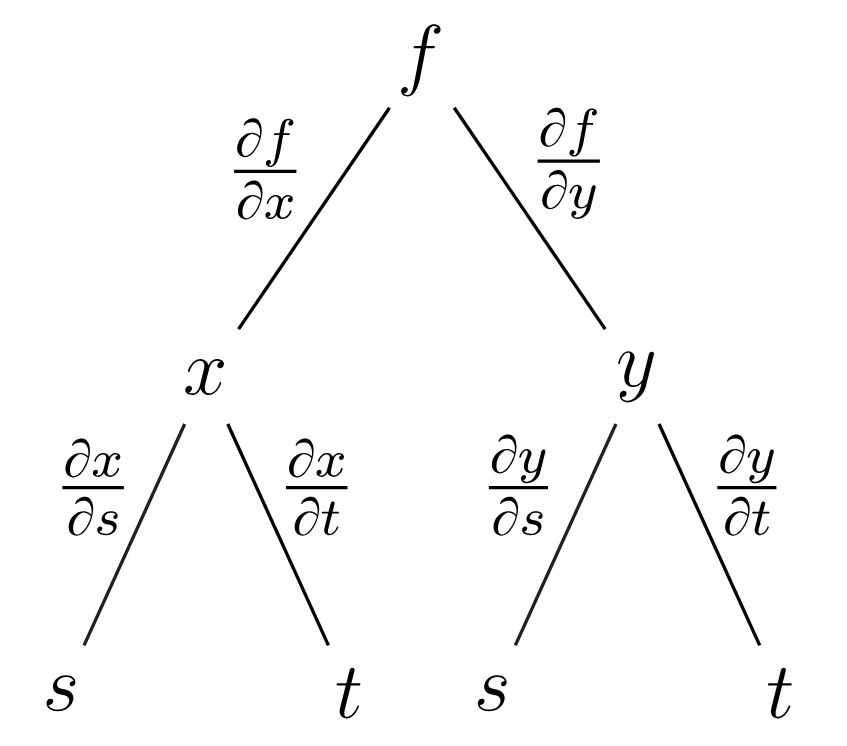
\includegraphics[width=0.75\linewidth]{chapters/chapter 7/chain rule.png}
\end{marginfigure}


\begin{example}
Ենթադրենք $f(x,y)=\sin(x^2+y^2)$, $x=t^2+3$ և
$y=t^3$: Այդ դեպքում՝
\begin{align*}
{f_t}&=f_xx_t+f_yy_t=(2x \cos(x^2+y^2))\cdot (2t)+(2y \cos(x^2+y^2))\cdot(3t^2)\\&=4xt\cos(x^2+y^2)+6yt^2\cos(x^2+y^2)
\end{align*}
Մնում է միայն տեղադրել $x$-ի ու $y$-ի արժեքները։
\end{example}

\begin{example}
Եթե ունենք միայն մեկ փոփոխական՝
\[z(x) = x^2 + 4x\]  
որը կախված է մի ուրիշից՝ \[x(t) = 5t^3 + 2t\]
շղթայի կանոնը դառնում է նույնը, ինչ բարդ ֆունկցիայի ածանցման կանոնը՝ $z(x(t))'=z'(x(t)) \cdot x'(t)$։ Ունենում ենք՝
\begin{align*}
z_t &= z_xx_t= (2x+4)\cdot (15t^2+2)\\&=(2\cdot (5t^3 + 2t)+4)\cdot (15t^2+2)=150 t^5 + 80 t^3 + 60 t^2 + 8 t + 8
\end{align*}
\end{example}

\question{Կարո՞ղ եք ասել այնպիսի ֆունկցիա, որի գրադիենտն է $[2xy \quad x^2+4]$:}


\section{Ուղղությամբ ածանցյալ}

Մի քանի փոփոխական (հետևաբար նաև՝ մի քանի կոորդինատային առանցքներ) ունենալու լավն այն է, որ կարող ենք քայլել լիքը տարբեր ուղղություններով, ոչ թե միայն աջ կամ ձախ։ Մինչդեռ մասնակի ածանցյալները ցույց են տալիս միայն, թե որքան է ֆունկցիայի արա\-գությունը տվյալ կոորդինատային առանցքի երկայնքով շարժվելիս՝ \marginnote{ասենք՝ $f_x$-ը $f$-ի արագությունն է՝ $x$-երի առանցքով աջ ու ձախ շարժվելիս} մնացած բոլոր կոորդինատները թողնելով ֆիքսած։ Իսկ ի՞նչ, եթե ուզում ենք շարժվել ինչ-որ միջանկյալ ուղղությամբ, այսինքն՝ միաժամանակ փոփոխելով մի քանի փոփոխականներ։

Այլ կերպ ասած՝ ի՞նչ կլինի, եթե որոշեք միաժամանակ փոխել և սուրճի, և թեյի գինը, ասենք՝ սուրճը թանկացնեք $h$ դրամով, իսկ թեյը՝ դրանից երկու անգամ ավել, $2h$ դրամով։ Եկամտի ֆունկցիայի արգումենտը այդ դեպքում կդառնա՝
\[
\begin{bmatrix}
    x \\ y
\end{bmatrix}
\mapsto 
\begin{bmatrix}
    x + h \\ y + 2h
\end{bmatrix}
\]
այսինքն՝ կշարժվի $\vv = \begin{bmatrix}
    1 & 2
\end{bmatrix}$ վեկտորի ուղղությամբ ($h$ չափով)։ Ուրեմն ֆունկցիայի/եկամտի փոփոխությունը կկազմի՝
\[
f(\vx+h\vv)-f(\vx)
\]
որը, ինչպես կռահում եք, կբաժանենք փոփոխության չափի՝ $h\|\vv\|$-ի վրա, որպեսզի գտնենք միավոր փոփոխությունը՝
\[
\frac{f(\vx+h\vv)-f(\vx)}{h\|\vv\|}
\]
և վերջապես ի՞նչ եք կարծում, ի՞նչ կանենք, որպեսզի ստանանք $\vv$ ուղղությամբ ֆունկցիայի փոփոխության արագությունը։

\begin{definition}
Ենթադրենք $f(\vx)=f(x_1, \dots, x_n)$ որևէ ֆունկցիա է, իսկ $\vv$-ն՝ որևէ $n$-չափանի վեկտոր։
Եթե հետևյալ սահմանը գոյություն ունի և անվերջ չէ՝\marginnote[*+2]{նշանակում են նաև $D_\vv f$ կամ $\partial_\vv f$}
\[
\nabla_{\vv}{f}(\vx) = \lim_{h \to 0} \frac{f(\vx + h\vv) - f(\vx)}{h\|\vv\|}
\]
ապա այն կանվանենք \textbf{$\vv$-ի ուղղությամբ ածանցյալ} $\vx$ կետում։
\end{definition}

Հարմարության համար սովորաբար կպահանջենք, որ $\vv$ վեկտորի երկարությունը լինի $1$։ Օրինակ $\begin{bmatrix}
    1 & 2
\end{bmatrix}$ վեկտորի փոխարեն կվերցնենք իրեն՝ բաժանած իր երկարության վրա՝ $\begin{bmatrix}
    \dfrac{1}{\sqrt{5}} & \dfrac{2}{\sqrt{5}}
\end{bmatrix}$, և այդ դեպքում $\nabla_\vv f(\vx)$-ի արժեքը չի փոխվի, իսկ հայտարարի $\|\vv\|$-ն կվերանա՝
\[
\nabla_{\vv}{f}(\vx) = \lim_{h \to 0} \frac{f(\vx + h\vv) - f(\vx)}{h} 
\qquad 
\text{(երբ $\|\vv\|=1$)}
\]

\warning{Ի տարբերություն $\nabla f$-ի՝ $\nabla_\vv f$-ը թիվ է, այլ ոչ վեկտոր։ Այն նույնպես տարբեր $\vx$-երում ընդունում է տարբեր արժեքներ։}
\question{Որո՞նք են $[1 \quad 0]$-ի և $[0 \quad 1]$-ի ուղղությամբ ածանցյալները։}


\begin{marginfigure}
    \centering
    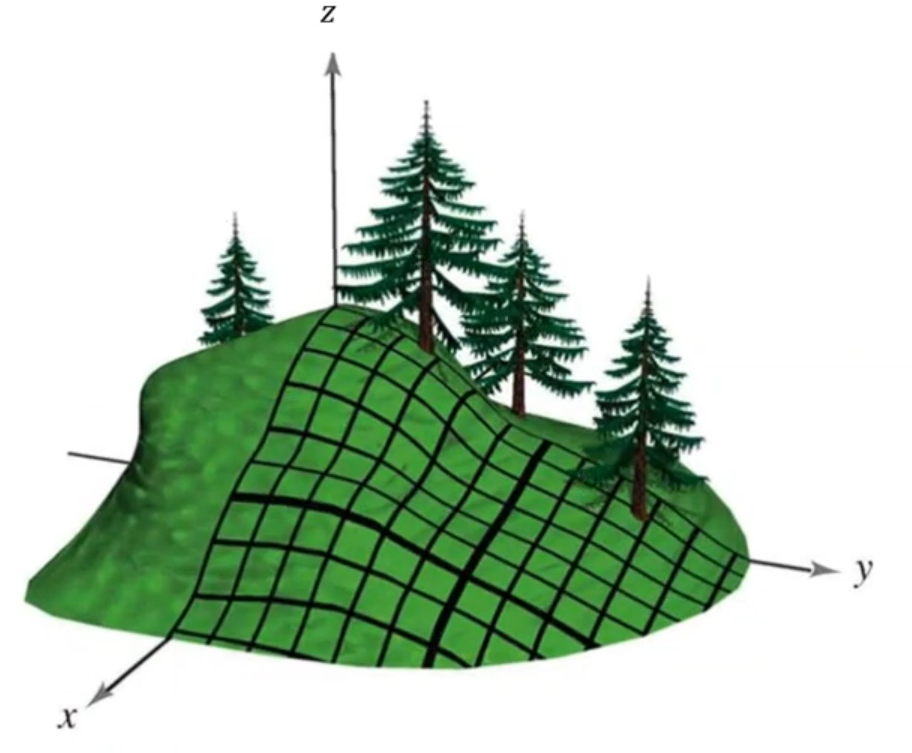
\includegraphics[width=\linewidth]{chapters/chapter 7/forest and peace.png}
\end{marginfigure}

Եթե պատկերացնենք, որ $f(x,y)$-ի գրաֆիկն, ասենք, սարի մակերևույթն է (լանջերը), ապա $xy$-հարթության մեջ գտնվող ցանկացած $\vv$ ուղղու\-թյամբ շարժվելիս սարի լանջով կամ կբարձրանանք, կամ կիջնենք։ $\nabla_\vv f$-ը ցույց է տալիս, թե որքան կկազմի բարձրանալ/իջնելու չափը, եթե մի փոքր քայլ անենք $\vv$ վեկտորի ուղղությամբ։ 

\question{Կարո՞ղ եք գուշակել, թե ինչպես է $\vv=[1 \quad 2]$-ի ուղղությամբ ածանցյալն արտահայտվում ըստ սուրճի ու թեյի գների մասնակի ածանցյալներով։}

Վերոնշյալ $\vv$ վեկտորի ուղղությամբ ածանցելիս, օրինակ, երկրորդ փոփոխականի արժեքը փոփոխում ենք $2$ անգամ ավելի չափով, քան առաջինը, հետևաբար ինչ-որ իմաստով՝ երկրորդի փոփոխման արագությունը պետք է երկու անգամ ավելի մեծ կարևորություն զբաղեցնի, քան առաջինինը։ Պարզվում է, որ իրոք, $\vv$ վեկտորի ուղղությամբ ածանցյալը կարող ենք արտահայտել $\vv$-ի բաղադրիչներով և $f$-ի մասնակի ածանցյալներով հետևյալ կերպ․

\begin{theorem}
Եթե $f$-ը դիֆերենցելի է $\vx$ կետում և $\|\vv\|=1$, ապա
\[
\nabla_\vv f(\vx) = f_{x_1}v_1 + f_{x_2}v_2 + \dots + f_{x_n}v_n
\]
այսինքն՝
\[
\nabla_\vv f(\vx) = \nabla f(\vx_0) \cdot \vv
\]
\end{theorem}

\question{\href{https://www.geogebra.org/m/Bx8nFMNc}{Խաղալով} $P$-ի դիրքի և $\vu$-ի ուղղության հետ՝ կարո՞ղ եք պարզել, թե որ ուղղությամբ է ածանցյալն ամենամեծը։}


\section{Գրադիենտը երկրաչափորեն}

Եթե պատկերացնեք, որ գտնվում եք սարի վրա, որը Ձեր եկամտի ֆունկցիայի գրաֆիկն է (կամ եթե պարզապես ուզում եք բարձրանալ սարի գագաթը), առաջին բանը, որ կուզեք անել՝ Ձեր կանգնած դիրքից շարժվել հնարավորինս վեր։ Այսինքն՝ գրաֆիկասարի յուրաքանչյուր կետում բոլոր հնարավոր ուղղություններից կընտրեք այն ուղղությունը, որով քայլելիս ամենաշատը կբարձրանաք, և կքայլեք այդ ուղղությամբ։ 

Իսկ ինչպե՞ս հասկանանք, թե տվյալ $\vx$ կետում ո՞ր $\vv$ ուղղությամբ գնալիս ենք ամենաշատը բարձրանում, կամ որ նույնն է՝ ո՞ր ուղղությամբ է ֆունկցիայի ածանցյալն ամենամեծը։

\begin{figure}[t]
    \centering
    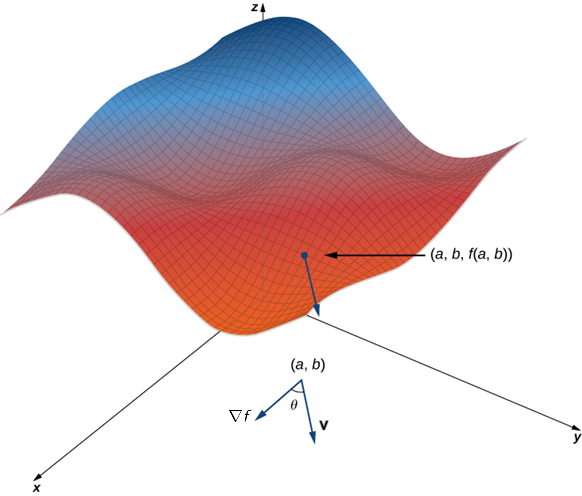
\includegraphics[width=0.75\linewidth]{chapters/chapter 7/grad angle.png}
    \caption*{գտնվում ենք $(a,b)$ կետում}
\end{figure}

Ենթադրենք շարժվում ենք $\vv$ ուղղությամբ և $\|\vv\|=1$: Այդ ուղղությամբ ածանցյալը կլինի՝
\[
\nabla_{\vv}f=\nabla f\cdot \vv
\]
որը, եթե $\nabla f$-ի ու $\vv$-ի կազմած անկյունը նշանակենք $\theta$-ով, կդառնա՝
\[
\|\nabla f\|\cdot \|\vv\| \cdot \cos\theta=  \|\nabla f\|\cos\theta
\]

Բայց $-1 \le \cos\theta \le 1$, հետևաբար $\nabla_\vv f$-ը ամենաշատը կարող է լինել $\|\nabla f\|$, դա էլ միայն այն դեպքում, երբ $\cos\theta$-ն հավասար լինի $1$-ի։ Իսկ 
\[
\cos\theta=1
\quad \text{ նշանակում է } \quad
\theta = 0
\]
և $\vv$-ի ու $\nabla f$-ի ուղղությունները \textit{համընկնում են։} Ստացվեց, որ

\begin{theorem}
\marginnote{ամենադիք վերև ուղղված ուղղությունը} Գրադիենտը ցույց է տալիս ֆունկցիայի \textbf{ամենաարագ աճման ուղղությունը։}
\end{theorem}

Այսինքն եթե գտնվում ենք $(a,b)$ կետում, ապա հաշվելով $\nabla f(a,b)$-ն ու քայլելով ստացված վեկտորի ուղղությամբ՝ կունենանք հնարավոր ամենամեծ աճը։

\question{Իսկ ո՞րն է ֆունկցիայի ամենաարագ \textbf{նվազման} ուղ\-ղու\-թյունը։}

\warning{Հիշենք, որ ածանցյալները ցույց են տալիս ֆունկցիայի աճել/նվազելը միայն տրված կետի մոտիկ շրջակայքում․ $\nabla f$-ի ուղ\-ղությամբ շատ մեծ քայլ անելիս ֆունկցիան կարող է չմեծանալ։}

Սա երկրաչափորեն մեկնաբանում է, թե ինչ վեկտոր է գրադիենտը՝
\begin{itemize}
    \item ուղղությունը $=$ ամենակտրուկ բարձրանալու ուղղությունը
    \item երկարությունը $=$ այդ ուղղությամբ ֆունկցիայի արագությունը
\end{itemize}
և առանցքային դեր է խաղում օպտիմիզացիայի տեսության ու մեքե\-նայական ուսուցման մեջ։


\section{Էքստրեմումի խնդիրը բազմաչափ դեպքում}

Ճիշտ ինչպես \hyperref[single_var_extrema]{\color{OliveGreen}միաչափ դեպքում} ածանցյալի միջոցով որոնում ու գտնում էինք, թե որ կետերում է ֆունկցիան ընդունում իր լոկալ իմաստով ամենամեծ/ամենափոքր արժեքները, նույնը կարող ենք անել նաև այս դեպքում՝ ածանցյալի փոխարեն օգտագործելով դրա բազմաչափ տարբերակը՝ ֆունկցիայի գրադիենտը։

Ենթադրենք ունենք որևէ $f(\vx)=f(x_1,\dots,x_n)$ ֆունկցիա։

\begin{definition}
Կասենք, որ $f(\vx)$-ը $\va$ կետում ընդունում է \textbf{լոկալ մաքսիմում} (մինիմում), եթե $\va$ կետին բավականաչափ մոտ՝\marginnote[*+1.5]{այսինքն՝ $\va$-ից ամենաշատը $\delta$ հեռա\-վորության վրա գտնվող կետերում}
\[
\|\vx-\va\| < \delta
\]
կետերում $f$-ի ամենամեծ (ամենափոքր) արժեքը $f(\va)$-ն է։
\end{definition}

$\va$ կետը համապատասխանաբար կանվանենք ֆունկցիայի \textit{լոկալ մաք\-սի\-մումի (մինիմումի) կետ,} իսկ այդ երկուսը միասին՝ \textit{էքստրե\-մու\-մի կետեր։} Նման ձևով կսահմանենք նաև գլոբալ էքստրեմումի ու կրիտի\-կական կետի գաղափարները։ 


\begin{figure}[b]
\centering %
\floatsetup{floatrowsep=qquad}
\begin{floatrow}[3]%
\ffigbox[\FBwidth]{\caption*{\centering լոկալ մաքսիմում}}{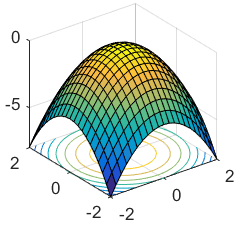
\includegraphics[width=0.4\textwidth]{chapters/chapter 7/local max.png}}
\ffigbox[\FBwidth]{\caption*{\centering լոկալ մինիմում}}{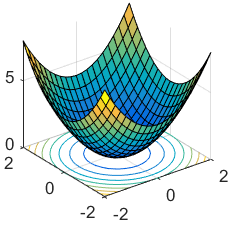
\includegraphics[width=0.4\textwidth]{chapters/chapter 7/local min.png}}
\ffigbox[\FBwidth]{\caption*{\centering թամբի կետ}}{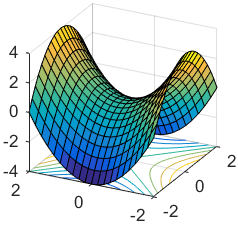
\includegraphics[width=0.4\textwidth]{chapters/chapter 7/saddle point.png}}
\end{floatrow}
\end{figure}


Ինչպես մեկ փոփոխականի ֆունկցիայի դեպքում, այնպես էլ այստեղ․
\begin{theorem}
Եթե $\va$-ն $f$-ի լոկալ կամ գլոբալ էքստրեմումի կետ է և $f$-ը $\va$-ում դիֆերենցելի է, ապա
\[
\nabla f(\va) = \mathbf{0}
\]
\end{theorem}

Եվ նորից, այս պայմանը անհրաժեշտ է, բայց ոչ՝ բավարար․ կրիտի\-կա\-կան կետ լինելը դեռ չի նշանակում, որ կետը էքստրեմումի կետ է։ Այլ կերպ ասած՝ հնարավոր է, որ որևիցե կետում ֆունկցիայի գրադիենտը լինի $\mathbf{0}$, բայց ֆունկցիան չընդունի ոչ լոկալ մաքսիմում, ոչ լոկալ մինիմում։ Այդպիսի կետերը կանվանենք \textit{թամբի կետեր։}

\newpage

\begin{definition}
Կասենք, որ $\va$-ն $f$ ֆունկցիայի\marginnote{անգլերեն՝ {\it saddle point}} \textbf{թամբի կետ} է, եթե այն էքստրեմումի կետ չէ, բայց $\nabla f(\va) = \mathbf{0}$։
\end{definition}

Ինչո՞ւ է կոչվում թամբի կետ։ Որովհետև \href{https://math.libretexts.org/Courses/University_of_California_Davis/UCD_Mat_21C\%3A_Multivariate_Calculus/13\%3A_Partial_Derivatives/13.7\%3A_Extreme_Values_and_Saddle_Points#Second_Derivative_Test_2:~:text=appears\%20in\%20the\%20following\%20figure.}{նման է} թամբի։ Կարող էր կոչվել նաև չիփսի կետ։

\begin{marginfigure}
    \centering
    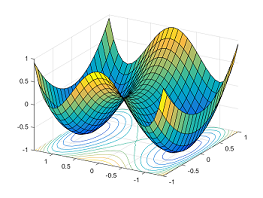
\includegraphics[width=\linewidth]{chapters/chapter 7/many critical points.png}
    \caption*{տիպիկ ֆունկցիա՝ լիքը կրիտիկական կետերով}
\end{marginfigure}

Նման կետերում ֆունկցիայի գրադիենտը զրո է (այսինքն՝ բոլոր մասնակի ածանցյալները $= 0$), սակայն մի փոփոխականը ֆիքսած մյուսը փոփոխելիս՝ ֆունկցիան աճում է, իսկ սա ֆիքսելով՝ առաջինը փոփոխելիս՝ նվազում։ Արդյունքում ստացվում է, որ ֆունկցիան այդ կետում ոչ մեծագույն արժեք է ընդունում, ոչ փոքրագույն։

Որպեսզի պարզենք, թե $f(x,y)$-ի կրիտիկական կետերից որոնք են լոկալ էքստրեմումներ, կօգտվենք նմանատիպ մի արդյունքից, ինչ մեկ փոփոխականի ժամանակ։ Վերցնենք $f$-ի մասնակի ածանցյալները՝ $f_x(x,y)$ և $f_y(x,y)$, ու ածանցենք դրանք ևս մեկ անգամ՝ ըստ յուրաքան\-չյուր փոփոխականի։ Ածանցելով
\begin{itemize}
    \item $f_x$-ը՝ կստանանք $f_{xx} = (f_x)_x$ և $f_{xy} = (f_x)_y$
    \item $f_y$-ը՝ կստանանք $f_{yx} = (f_y)_x$ և $f_{yy} = (f_y)_y$
\end{itemize}
ընդ որում եթե ստացված ածանցյալներն անընդհատ են, ապա ածանց\-ման հերթականությունը կարևոր չէ՝ $f_{xy} = f_{yx}$։

Այժմ հետևյալ մատրիցի՝ \marginnote[*+0.5]{որը կոչվում է $f$-ի \textit{հեսիան}}
\[
    \begin{bmatrix}
        f_{xx} & f_{xy} \\
        f_{yx} & f_{yy}
    \end{bmatrix}
\]
որոշիչը նշանակենք $D$-ով․
\[
D = f_{xx}f_{yy}-f_{xy}^2
\]

Եթե մեկ փոփոխականի դեպքում $f''$-ի նշանը ցույց էր տալիս՝ տրված կրիտիկական կետը էքստրեմումի կետ է, թե ոչ, ապա երկու փոփոխականի դեպքում նույն բանը անում է $D$-ի նշանը։

\begin{theorem}
Եթե $\nabla f(\va) = \mathbf{0}$ ու
\begin{itemize}
    \item $D>0$ և $f_{xx}>0$, ապա $\va$-ն լոկալ մինիմումի կետ է
    \item $D>0$ և $f_{xx}<0$, ապա $\va$-ն լոկալ մաքսիմումի կետ է
    \item $D<0$, ապա $\va$-ն թամբի կետ է
\end{itemize}
\end{theorem}

Նկատենք, որ այս դեպքում ևս $D=0$ կամ $f_{xx}=0$ դեպքերի մասին թեորեմը ոչինչ չի կարող ասել։





\bigskip 

\begin{theory}
.
\begin{itemize}
\item կարդալ [{\rm Stewart}], 880-883 (գրաֆիկ), 900-905 (մասնակի ածանցյալ), 924-925 (շղթայի կանոն), 933-937 (ուղղությամբ ածանցյալ), 946-949 (էքստրեմումներ) էջերը
\item տեսնել մասնակի ածանցյալներն ու գրադիենտը \href{https://youtu.be/GkB4vW16QHI}{սե\-փա\-կան աչքով}
\item ըստ ցանկության՝ դիտել Բ․ Մալթսբիի ներածական \href{https://www.youtube.com/playlist?list=PLBEl4BT8wUgP9lAPqVzuytn09oV_xqTIJ}{տեսա\-դա\-սերը} շատ փոփոխականի ֆունկցիաների մասին 
\item ինչպես նաև Կ․ Քեռյանի խորացված \href{https://www.youtube.com/playlist?list=PLz3NrXxHz_CBamqkX-nPy-hN2iaHmouyo}{դասախոսություններից} 8-րդ և 11-րդ դասերը
\end{itemize}
\end{theory}

\newpage

\section{Խնդիրներ}


\begin{problem}
Հետևյալ ֆունկցիաները համապատասխանեցրեք իրենց գրաֆիկներին․
\begin{enumerate}[label={\alph*}․]
\item $f(x,y) = |x| + |y|$
\item $f(x,y) = |xy|$
\item $f(x,y) = \dfrac{1}{1+x^2+y^2}$
\item $f(x,y) = (x^2-y^2)^2$
\item $f(x,y) = (x-y)^2$
\item $f(x,y) = \sin\left(|x|+|y|\right)$
\end{enumerate}

\begin{figure}[h]
\centering
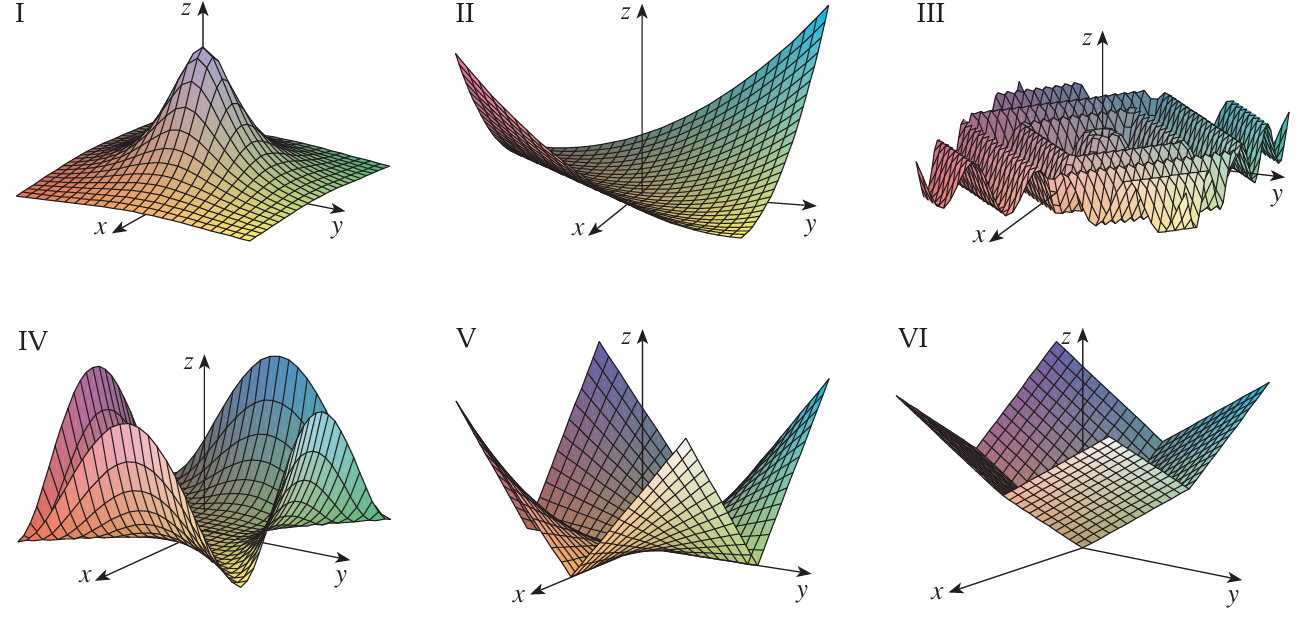
\includegraphics[width=0.75\linewidth]{chapters/chapter 7/match graph.png}
\end{figure}
\end{problem}


\begin{problem}
Գտեք ֆունկցիայի մասնակի ածանցյալները․
\begin{enumerate}[label={\alph*}․]
\item $f(x,y)=3x-2y^2$
\item $f(x,y)=y^7-2x^3+x^2$
\item $f(x,y)=\sin{(xy)}$
\item $f(x,y)=x \cdot \ln y+\dfrac{x}{y}$
\end{enumerate}
\end{problem}


\begin{problem}
Որքա՞ն է $\vv=\begin{bmatrix}
    0.6 & 0.8
\end{bmatrix}$ վեկտորի ուղղությամբ ածանցյալը $(-1,-1)$ կետում․
\begin{enumerate}[label={\alph*}․]
\item $f(x,y) = 3xy$
\item $f(x,y) = 1-x^2$
\item $f(x,y) = e^{x-y}$
\end{enumerate}
\end{problem}


\begin{problem}
Սևանա լճի $(x, y)$ կոորդինատներով կետում ջրի խորությունը 
\[xy^{2}-6x^{2}-3y^{2}\]
մետր է։ $(5, 3)$ կետում գտնվող «Նորատուս» առագաստանավի նավա\-պետը ցանկանում է շարժվել դեպի մի այնպիսի կետ, որում ջուրն ավելի խոր է։ Նրա առաջին օգնականն առաջարկում է նավարկել դեպի հյուսիս, իսկ երկրորդը՝ դեպի հարավ։ Օգնականներից որի՞ խորհուրդը պետք է լսի նավապետը։
\end{problem}


\begin{problem}
Որո՞նք են ֆունկցիայի լոկալ մինիմումի և մաքսիմումի կետերը (եթե կան)․
\begin{enumerate}[label={\alph*}․]
\item $f(x, y) = 3xy$
\item $f(x, y) = x^2-xy$
\item $f(x, y) = 2x^2 - x^3 - y^2$
\item $f(x, y) = x^3 - 3x - y^3 + 3y$
\end{enumerate}
\end{problem}


\begin{problem}
Անհրաժեշտ է $(-5, 0)$, $(1, 7)$, $(9, 0)$ և $(0, -8)$ կոորդինատնե\-րով կետերում գտնվող չորս գյուղերի համար կառուցել հեռուստաաշտարակ։ Ո՞ր $(x, y)$ կետում կառուցենք աշտարակը, որպեսզի գյուղերից դրա ունեցած հեռավորությունների քառակուսիների գումարը լինի հնարա\-վորինս փոքր։
\end{problem}

\hint{Կոորդինատային հարթության մեջ պատկերեք կետերը և գրեք դրանց հեռավորությունը $(x,y)$ կետից։ Ինչի՞ է հավասար դրանց քառակուսիների գումարը։}


\begin{problem}
Ունենք $12$ մ$^2$ մակերեսով ստվարաթուղթ (ինչպես նաև մկրատ ու սոսինձ), որով այս անգամ ցանկանում ենք պատրաստել այսպիսի բաց տուփ (այսինքն առանց վերևի նիստի)՝
\begin{figure}[h]
    \centering
    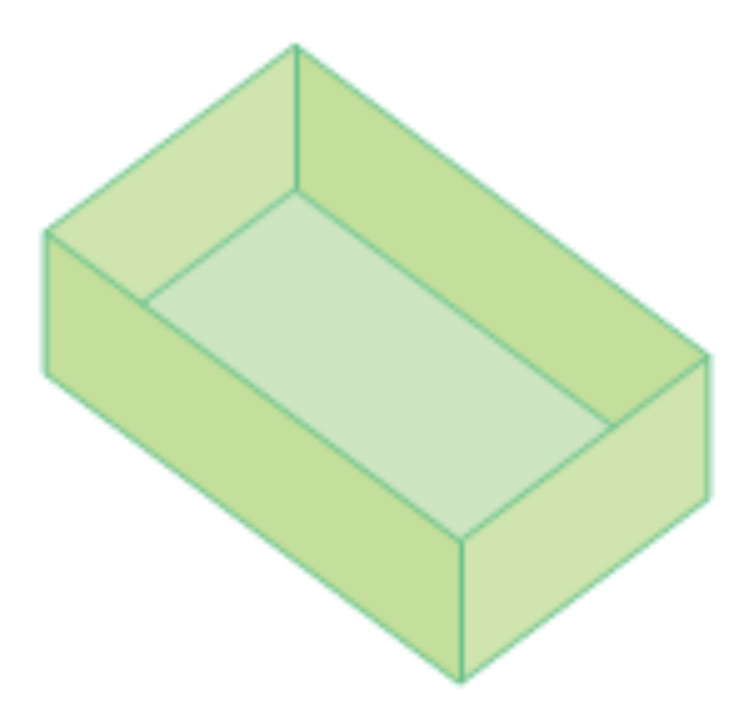
\includegraphics[width=0.4\linewidth]{chapters/chapter 7/topless-box.png}
\end{figure}

Ամենաշատը որքա՞ն կարող է լինել այդ տուփի ծավալը։

\hint{Այս անգամ քառակուսիներ չկան, հետևաբար նշանակենք խորանարդի կողմերը $x$, $y$ և $z$: Կարո՞ղ եք $z$-ն արտահայտել $x$-ով ու $y$-ով։ Իսկ ծավալը՞։}
\end{problem}

\setchapterpreamble[u]{\margintoc}
\chapter{Հավանականություն}
\labch{probability}

\emergencystretch 2em

\section{Պատահական փորձ}

Հաճախ կյանքում հանդիպում ենք այնպիսի իրավիճակների, երբ այս կամ այն գործողության/երևույթի արդյունքը հնարավոր չէ գուշակել, ասենք՝
\begin{itemize}
    \item ի՞նչ թիվ կընկնի, եթե նետենք զառը
    \item ո՞ր կողմի վրա կընկնի նետված մետաղադրամը
    \item ո՞վ կհաղթի, եթե շախմատ խաղաք Լևոն Արոնյանի հետ
    \item եթե դուրս գանք փողոց ու կանգնեցնենք պատահական անցորդի, ի՞նչ կլինի նրա անունը
    \item եթե դուրս գանք փողոց ու կանգնեցնենք պատահական անցորդի, որքա՞ն կլինի նրա հասակը
    \item քանի՞ րոպեից կժամանի $62$ համարի ավտոբուսը
\end{itemize}
և այլն։ Իրոք, մինչև զառը չնետենք, կանգառում չսպասենք, խաղը չխաղանք՝ չենք կարող ասել հստակ արդյունքը։ 
Չնայած դրան՝ կարող ենք այնուամենայնիվ ինչ-որ ենթադրություններ անել հնարավոր արդյունքի մասին, այսինքն՝ համեմատել, թե հնարավոր ելքերից որը ավելի մեծ շանս ունի  տեղի ունենալու, որը՝ ավելի փոքր։ 

Այլ կերպ ասած՝ թեև հնարավոր չէ հստակ գուշակել արդյունքը, բայց կարելի է խոսել հնարավոր ելքերի \textit{հավանականությունների} մասին։ Օրինակ՝
\begin{itemize}
    \item \textit{զառ նետելիս}  

    \begin{itemize}
        \item[-] հնարավոր է վեց տարբերակ՝\marginnote{տարբերակներից յուրաքանչյուրը կան\-վա\-նենք \textit{տարրական ելք} կամ պար\-զա\-պես՝ \textit{ելք}} $1$, $2$, $3$, $4$, $5$ կամ $6$
        
        \item[-] քանի որ դրանցից ոչ մեկը մյուսի նկատմամբ առավելություն չունի, ապա բոլոր ելքերն ունեն նույն հավանականությունը
    \end{itemize}

    \item \textit{մետաղադրամ նետելիս} 

    \begin{itemize}
        \item[-] կա երկու ելք՝ գիր կամ ղուշ
        
        \item[-] եթե մետաղադրամը իսկական է, երկու ելքերի դուրս գալու հավանականությունը նույնն է՝ $50\%$-ով գիր, $50\%$-ով՝ ղուշ

        \item[-] հնարավոր է, որ մետաղադրամը կեղծված լինի այնպես, որ այն ավելի հակված լինի ասենք՝ ընկնելու գիր․ այդ դեպքում գիր ընկնելու հավանականությունն ավելի մեծ կլինի, քան ղուշ ընկնելունը
    \end{itemize}

    \item \textit{շախմատ խաղալիս}

    \begin{itemize}
        \item[-] կա երկու ելք՝ հաղթում եք կամ Դուք, կամ Լևոն Արոնյանը
        \item[-] գրեթե $100\%$-անոց հավանականությամբ հաղթողը կլինի Արոնյանը
    \end{itemize}
    
    \item \textit{պատահական մարդու անունը հարցնելիս}

    \begin{itemize}
        \item[-] կան հարյուր հազարավոր հնարավոր ելքեր
        \item[-] դրանցից որոշները (ասենք՝ Անի կամ Դավիթ) ավելի հավանական են, քան մյուսները
        \item[-] միջինում $1000$ անցորդից մոտ $20$-ի անունը կլինի Անահիտ, ևս $17$-ինը՝ Արմեն, և այլն
    \end{itemize}
        
    \item \textit{պատահական մարդու հասակը հարցնելիս}

    \begin{itemize}
        \item[-] կան անվերջ թվով ելքեր․ մարդու հասակը կարող է լինել, ասենք, \marginnote{նկատի ունենք ճշգրիտ հասակը (նանո\-մետ\-րերի ճշտությամբ), ոչ կլորացված} $(60, 240)$ սմ միջակայքից ցանկացած թիվ 
        \item[-] ավելի հավանական է, որ հասակները լինեն $(160, 180)$ միջակայքում, քան ասենք՝ $(210, 230)$
    \end{itemize}

    \item \textit{$62$ համարի ավտոբուսին սպասելիս}

    \begin{itemize}
        \item[-] այս հարցին հավանականությունների տեսությունն անզոր է պատասխանել
    \end{itemize}
\end{itemize}
\question{Ի՞նչ եք կարծում, որքա՞ն է հավանականությունը, որ պատա\-հական վերցված մարդու հասակը լինի $174.12345678912345...$ սմ։} 
Յուրաքանչյուր այսպիսի երևույթ կանվանենք \textit{պատահական փորձ} ($=$ բան, որի ելքը/արդյունքը չգիտենք)։ Ամեն մի պատահական փորձի համար նրա բոլոր հնարավոր ելքերը կհավաքենք մեկ բազմության մեջ և կանվանենք այն \textit{բոլոր ելքերի բազմություն} կամ \marginnote{անգլերեն՝ {\it sample space}} \textit{նմուշային տարածություն} (կնշանակենք $\Omega$ տառով)․
\[
\Omega = \{ \text{տվյալ պատահական փորձի բոլոր հնարավոր ելքերը} \}
\]

\begin{example}
Մետաղադրամ նետելը պատահական փորձ է, որի ելքերն են՝\marginnote{անգլերեն՝ {\it heads} և {\it tails}}
\[
\Omega = \{\text{գիր}, \text{ղուշ}\} = \{\text{Գ}, \text{Ղ}\} = \{{\rm H}, {\rm T}\}  
\]
\end{example}

\begin{example}
Ցանկացած ֆուտբոլային խաղ պատահական փորձ է, որի ելքը խաղի հաշիվն է․ քանի դեռ խաղը տեղի չի ունեցել, հաշիվը չգիտենք։ Եթե պայմանավորվենք օրինակ՝
\[
\text{Փյունիկ } 2 - 1 \text{ Ալաշկերտ}
\]
ելքը նշանակել $(2, 1)$-ով, բոլոր ելքերը կլինեն՝
\[
\Omega = \{(0,0),\ (0,1),\ (1,0),\ (1,1),\ (2,0),\ \dots \}
\]
\end{example}

\begin{example}
Եթե պատահական ինչ-որ պահի դուրս գաք կանգառ և սպասեք, թե քանի րոպեից կգա ավտոբուսը, դա նույնպես կլինի պատահական փորձ։ 

Եթե համարենք, որ ավտոբուսներն անցնում են ժամը մեկ, հնարավոր է, որ հաջորդ ավտոբուսը գա $45$ րոպե անց, հնարավոր է՝ կես ժամ կամ $29.5$ րոպե անց, կամ միգուցե՝ $\pi$ րոպե անց․
\[
\Omega = (0, 60)
\]
Նորից, պայմանավորվենք ավտոբուսի գալու ժամանակը չկլորացնել րոպեի ճշտությամբ\marginnote{այսինքն՝ $\pi$ րոպե $\ne 3$ կամ $3.14$ րոպե}։ Բայց այդ դեպքում $(0, 60)$ միջակայքում կան անվերջ քանակով թվեր, որոնցից ոչ մեկը մյուսների նկատմամբ առավելություն չունի։ Իրոք, ինչո՞ւ պիտի ավտոբուսի $35.1908470$ րոպե հետո գալու հավանականությունը ավելի փոքր կամ ավելի մեծ լինի, քան ասենք $35.1908480$ կամ $35.1908471$ րոպե հետո գալունը։ 

Ստացվում է, որ $(0, 60)$ միջակայքում կան անվերջ քանակով թվեր, և յուրաքանչյուրի տեղի ունենալու հավանականությունը նույնն է, ինչ մյուսներինը։ Ուրեմն (որքան էլ ոչ ինտուիտիվ թվա) ելքերից ցանկացածի հավանականությունը․․․ $0$ է։ 

Սա \textbf{չի նշանակում,} որ ոչ մի ելք հնարավոր չէ, և ավտոբուսը երբեք էլ չի գալու․ \marginnote{\href{https://www.youtu.be/ZA4JkHKZM50}{այս մասին ավելի համոզիչ}}\textit{հավանականությունը $0$ լինել} $\ne$ \textit{հնարավոր չլինել։} Պարզապես նստել ու սպասել, որ ավտոբուսը կգա հենց ուղիղ $35.1908480$ րոպե անց, և ոչ մի վայրկյան, միլիվայրկյան ու նանովայրկյան ուշ կամ շուտ, նման բանի տեղի ունենալու շանսերը զրոյական են։
\end{example}

Նկատենք, որ կախված փորձից՝ ելքերի բազմությունը կարող է տարբեր քանակությամբ տարրեր ունենալ․ առաջին օրինակում $\Omega$-ն երկու ելքից էր բաղկացած, երկրորդում (ըստ էության) ու երրորդում՝ անվերջ թվով ելքերից։ Ընդ որում եթե երրորդ օրինակում $\Omega$-ն միջակայք էր, ապա երկրորդում $\Omega$-ն բնական թվերի զույգերից բաղկացած բազմություն էր։ 

Նշենք, որ եթե բազմության տարրերը կարելի է բնական թվերով համարակալել (այսինքն՝ $1$-ին տարր, $2$-րդ տարր, $\dots$), ապա այն անվանում ենք \textit{հաշվելի,} իսկ եթե բազմությունը միջակայք է, ապա այն \href{https://www.youtu.be/nU3fzO94lBw}{չենք կարող} համարակալել և անվանում ենք \textit{անհաշվելի։} Սա է պատճառը, որ նման միջակայքերի դեպքում ունենք շատ-շատ մեծ քանակությամբ անվերջ հատ ելքեր, որոնցից յուրաքանչյուրի հավա\-նականությունը $0$ է, թեև դրանք բոլորն էլ հնարավոր ելքեր են։

% \question{}


\section{Պատահույթներ}

Եկեք այժմ ներմուծենք հավանականությունը հաշվելու համար ան\-հրա\-ժեշտ որոշակի գործիքներ։ 

Ենթադրենք նետում ենք զառ․
\[
\Omega=\{1,\, 2,\, 3,\, 4,\, 5,\, 6\}
\]
Կարող ենք, օրինակ, հարցնել՝ արդյո՞ք զառը կընկնի
\begin{itemize}
    \item $3$
    \item $1$ կամ $6$
    \item $4$-ից փոքր թիվ
    \item զույգ թիվ
    \item պարզ թիվ\marginnote{$2$, $3$, $5$ պարզ են, $4$ ու $6$-ը՝ բաղադրյալ, $1$-ը՝ ոչ պարզ, ոչ բաղադրյալ}
    \item բնական թիվ
    \item մի որևէ թիվ
    \item ոչ մի թիվ էլ չի ընկնի
\end{itemize}

\question{Ինչպե՞ս կպատասխանեիք վերջին երեք հարցերին։}

Յուրաքանչյուր դեպքում որոնվող հավանականությունը կնշանակենք $\PP$ տառով, ասենք՝
\[
\PP[\text{$1$ կամ $6$}] =\ ?
\]
կամ
\[
\PP[\text{պարզ թիվ}] =\ ?
\]

Որպեսզի էլ ավելի պարզեցնենք գրելաձևը, պայմանավորվենք բառերով «$1$ կամ $6$», «պարզ թիվ», և այլն գրելու փոխարեն ներկայացնել նշված պայմանին բավարարող թվերը \textit{բազմության} միջոցով, այսինքն՝
\[
\PP[\text{$1$ կամ $6$}]\text{-ի փոխարեն՝} \qquad 
\PP[\{1,\ 6\}]
\]
և
\[
\PP[\text{պարզ թիվ}]\text{-ի փոխարեն՝} \qquad 
\PP[\{2,\ 3,\ 5\}]
\]
քանի որ այսպես ավելի հարմար է։ Ցանկության դեպքում կարող ենք նաև այս բազմությունները նշանակել տառերով՝ $A=\{1, 6\}$ և $B=\{2, 3, 5\}$, ու պարզապես գրել՝ $\PP[A]$ և $\PP[B]$։

\question{Ո՞ր բազմությունով կներկայացնեք զույգ լինելու հարցը։ \linebreak Իսկ $3$ լինելո՞ւնը։}

Բոլոր այսպիսի հարց-բազմությունները կանվանենք \textit{պատահույթներ}\marginnote{անգլերեն՝ {\it event}}։ Փաստորեն դրանք տարրական ելքերից բաղկացած բազմություններ են, որոնց հավանականությունը փորձում ենք չափել․ եթե մեր դեպքում՝ $B=\{2, 3, 5\}$, ապա 
\[
\PP[\{2,\ 3,\ 5\}] \quad = \quad \text{հավանականությունը, որ ելքը $2$ կամ $3$ կամ $5$ է}
\]
այսինքն՝ որ ելքը $B$ բազմության տարրերից որևէ մեկն է։ Ելքի՝ զույգ թիվ լինելու պատահույթն էլ, օրինակ, կլինի $C=\{2, 4, 6\}$ բազմությունը։

\question{Ի՞նչ ցույց կտա $B \cap C$ պատահույթը։ Իսկ $A \cap B$՞-ն։}

Իրոք, ի՞նչ կլինի, եթե հատենք $B$ և $C$ բազմությունները․ կունենանք $B \cap C = \{2\}$, այսինքն՝ այն միակ ելքը, որը և՛ պարզ է ($B$ բազմությունից է), և՛ զույգ ($C$ բազմությունից է)․
\[
\PP[B \cap C] = \PP[\text{ելքը և՛ $B$-ից է, և՛ $C$-ից}]
\]
կամ այլ ձևով ասած՝ $B$-ի ու $C$-ի հատումը այդ երկուսի \textit{միաժամանակ} տեղի ունենալու պատահույթն է։

% \question{Ո՞րն է $A$ և $B$ պատահույթների հատումը։}

Նկատենք, որ երբեմն երկու պատահույթներ կարող են հատում չունենալ, օրինակ՝ $A$-ն ու $B$-ն, քանի որ չկա այնպիսի ելք, որը լինի և՛ պարզ, և՛ $\{1, 6\}$ բազմությունից։ Այդ դեպքում նրանց հատումը կլինի դատարկ բազմություն (որը նշանակում ենք $\varnothing$-ով), \marginnote{և իհարկե, եթե $A\cap B=\varnothing$, ապա դրանք միաժամանակ չեն կարող տեղի ունենալ՝ \[\PP[A \cap B] = 0\]} և կասենք, որ $A$ ու $B$ պատահույթներն \textit{անհամատեղելի} են կամ \textit{չհատվող}։

Նույն կերպ $B$-ի ու $C$-ի միավորումը՝ $B \cup C = \{2,\, 3,\, 4,\, 5,\, 6\}$ այն պատահույթն է, որ զառի թիվը կլինի պարզ կամ զույգ (կամ էլ երկուսը միաժամանակ)․
\[
\PP[B \cup C] = \PP[\text{ելքը կա՛մ $B$-ից է, կա՛մ $C$-ից}]
\]
կամ այլ ձևով ասած՝ $B$-ի ու $C$-ի հատումը այդ երկուսից \textit{գոնե մեկի} տեղի ունենալու պատահույթն է։

\begin{marginfigure}
    \centering
    \caption*{հարմար է պատահույթները ներ\-կա\-յաց\-նել այսպիսի շրջաններով}
    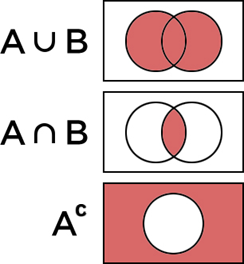
\includegraphics[width=0.75\linewidth]{chapters/chapter 8/set operations.png}
\end{marginfigure}

\warning{$B \cup C$-ում ներառված են նաև այն ելքերը, որոնք միաժամանակ երկուսին էլ պատկանում են։}

Վերջապես, եթե օրինակ՝ $B$-ն այն պատահույթն է, որ զառի ելքը պարզ է, ապա $B^c$-ով կնշանակենք դրա հակառակ պատահույթը, այսինքն՝ որ զառի ելքը պարզ \textit{չէ․}
\[
\PP[B^c] = \PP[\text{ելքը $B$-ից չէ}]
\]
Այս $B^c$ պատահույթը կանվանենք $B$ պատահույթի \textit{լրացում։} 

Նկատենք, որ ցանկացած $A$ պատահույթն ու իր $A^c$ լրացումը անհամա\-տե\-ղելի են՝ $A \cap A^c = \varnothing$, այսինքն՝ չի կարող ելքը և՛ պատկանել $A$-ին, և՛ չպատկանել $A$-ին (ասենք՝ և՛ զույգ լինել, և՛ զույգ չլինել)։

\question{Ի՞նչ կասեք $A \cup A^c$ պատահույթի մասին։ Ո՞ր բազմությունն է այն, և որքա՞ն պիտի լինի նրա հավանականությունը։}

Յուրաքանչյուր պատահական փորձի ժամանակ մեզ հետաքրքրող բոլոր պատահույթները կհավաքենք մեկ բազմության մեջ (որը կնշանակենք $\F$-ով) և այն \marginnote{անգլերեն՝ {\it event space}} կանվանենք \textit{պատահույթների տարածություն:} 

Նկատենք, որ այս $\F$-ի տարրերը բազմություններ են, այսինքն $\F$-ն ինքը բազմություններից բաղկացած բազմություն է:\marginnote{բոլորիս տանը կա տոպրակներով լցված տոպրակ․ $\F$-ը հենց այդ մեծ տոպրակն է} Քանի որ բոլոր հնարավոր ելքերի $\Omega$ բազմությունը նույնպես պատահույթ է, ապա $\Omega \in \F$։ 

Ընդհանուր առմամբ ինչպիսին էլ լինի մեր $\F$-ը, այն պետք է պարունակի ցանկացած պատահույթների հատումը, միավորումը և լրացումը․
\begin{enumerate}
    \item $\Omega$-ն և $\varnothing$-ը պատահույթներ են՝ $\Omega \in \F$, $\varnothing \in \F$

    \item ցանկացած $A$ պատահույթի լրացումը ևս պատահույթ է՝ $A^c \in \F$

    \item ցանկացած թվով պատահույթների հատումն ու միավորումը ևս պատահույթ է՝ 
    \begin{itemize}
        \item $A_1 \cap A_2 \in \F$
        \item $A_1 \cap A_2 \cap \dots \cap A_n \in \F$
        \item նույնիսկ անվերջ թվով՝ $\bigcap\limits_{n=1}^\infty A_n \in \F$
    \end{itemize}
    և
    \begin{itemize}
        \item $A_1 \cup A_2 \in \F$
        \item $A_1 \cup A_2 \cup \dots \cup A_n \in \F$
        \item նույնիսկ անվերջ թվով՝ $\bigcup\limits_{n=1}^\infty A_n \in \F$
    \end{itemize}
\end{enumerate}
կարճ ասած՝ հանգիստ կարող ենք ցանկացած գործողություն կատարել պատահույթների հետ, և արդյունքում ստացվածը կրկին անվանել «պատահույթ»։

\newpage

\question{Ենթադրենք $B$-ն զառի թվի պարզ, իսկ $C$-ն՝ զույգ լինելու պատահույթն է։ Կարո՞ղ եք $B$-ով ու $C$-ով արտահայտել պարզ, սակայն ոչ զույգ լինելու պատահույթը։}

Մինչև առաջ անցնելը նշենք, որ թեև միշտ կարող ենք հնարավոր ելքերից կազմված բոլոր բազմությունները համարել պատահույթներ ու անցնել առաջ,\marginnote{այդ դեպքում $\F$-ը կլինի $\Omega$-ի բոլոր ենթաբազմություններից բաղկացած գեր\-բազ\-մու\-թյունը} բայց երբեմն հարմար է լինում պաշտոնապես պատա\-հույթներ համարել միայն այն ելքերից բաղկացած բազմությունները, որոնք հետաքրքիր են տվյալ խնդրի տեսանկյունից։

\begin{example}
Պատկերացրեք՝ զառ ենք նետում, և եթե ընկնում է զույգ, ապա հաղթում ենք, եթե կենտ՝ պարտվում։ Այս դեպքում մեզ հետա\-քրքիր են հետևյալ երկու պատահույթների տեղի ունենալ-չունե\-նալը՝
\[
W = \{2, 4, 6\}, \qquad L = \{1, 3, 5\}
\]
և բացարձակապես հետաքրքիր չէ իմանալ՝ զառի վրայի թիվը պա՞րզ է, բաղադրյա՞լ է, $4$-ից մե՞ծ է, թե՞ $3$-ից փոքր։

Ուրեմն կարող ենք «անպետք տոպրակներն» աղբը նետել ու որպես պատահույթներ վերցնել միայն՝
\[ 
\F = \{ \varnothing,\ \{1,3,5\},\ \{2,4,6\},\ \Omega\} 
\]
\end{example}

\begin{example}
Իսկ եթե ասենք՝ նարդի խաղանք, և ինչ-որ պահի միակ հնարավոր թույլատրելի քայլը լինի $2$-ը, ապա նորից տարբերություն չկա՝ զառը կընկնի պարզ թիվ, թե բաղադրյալ․ կարևոր է միայն՝ $2$ կընկնի՞, թե՞ չի ընկնի։ 

Այսինքն՝ կարող ենք բավարարվել միայն $\{2\}$ պատահույթով և վերցնել՝
\[ 
\F = \{ \varnothing,\ \{2\},\ \{1,3,4,5,6\},\ \Omega\}
\]
\end{example}

Բարեբախտաբար, խնդիրներ լուծելիս պարտադիր չէ ամեն անգամ նշել, թե որն է $\F$-ը․ ավելորդ ֆորմալիզմից խուսափելու համար կարող ենք համարել, որ ելքերից կազմված ցանկացած բազմություն պատահույթ է, և լուծել խնդիրը։ Ավելի նուրբ դեպքերում, սակայն, սա կարող է հանգեցնել \href{https://www.youtu.be/wQQdpYhPTYM}{պարադոքսների}:


\section{Հավանականային չափ}

Բավական երկար ներածությունից հետո անցնենք մեր գլխավոր հերոսին՝ $\PP$-ին, որի միջոցով չափելու ենք բոլոր այն պատահույթների տեղի ունենալու հավանականությունները, որոնց մասին խոսեցինք վերևում։ Անվանենք այն \textit{հավանականային չափ։}\marginnote{անգլերեն՝ {\it probability measure}}

Ենթադրենք՝ կրկին նետում ենք զառը։ Կհամարենք, որ ամենամեծ («$100\%$-անոց») հավանականությունը $1$ է՝\marginnote[*+2]{նույն ինքը՝ $\PP[\Omega]=1$}
\[
\PP[\{1,\, 2,\, 3,\, 4,\, 5,\, 6\}] = 1
\]
և քանի որ բոլոր $6$ ելքերն ունեն միևնույն տեղի ունենալու հավանակա\-նությունը, դրանցից յուրաքանչյուրի հավանականությունը կլինի $\dfrac{1}{6}$՝
\newpage
\[
\PP[1]=\PP[2]=\dots=\PP[6]=\frac{1}{6}
\]
իսկ օրինակ զույգ թիվ ընկնելունը՝
\[
\PP[\{2,\, 4,\, 6\}] = \frac{3}{6} = \frac{1}{2}
\]

Նման դեպքերում, երբ ելքերից ոչ մեկի հավանականությունը մյուսից չի տարբերվում, ասում ենք, \marginnote{անգլերեն՝ {\it equiprobable}} որ բոլոր ելքերը \textit{հավասարահավանական} են։ Ինչպես վերևում տեսանք, հավասարահավանական դեպքում ցան\-կացած $A$ պատահույթի հավանականությունը հավասար է
\[
\PP[A] = \frac{\text{$A$-ի տարրերի թիվը}}{\text{բոլոր ելքերի թիվը}} = \frac{|A|}{|\Omega|}
\]

\begin{example}
Հիմա միաժամանակ նետենք երկու զառ։ Բոլոր տար\-բե\-րակները միասին՝ կունենանք $6\cdot 6 = 36$ հնարավոր ելք․
\[
\Omega = \{(x, y) \mid  1 \le x,\, y \le 6\}
\]
\marginnote{հերթականությունը կարևոր է․ $(3, 5)$ և $(5, 3)$ ելքերը \textbf{նույնը չեն}}Քանի որ դրանցից ցանկացածի տեղի ունենալու հավանականությունը նույնն է, ապա յուրաքանչյուր $(x, y)$ ելքի հավանականությունը կլինի՝
\[
\PP[(x, y)] = \frac{1}{36}
\]
իսկ օրինակ՝ երկուսի վրա էլ նույն թիվը լինելունը՝
\[
\PP[\{(1,1),\ (2,2),\ \dots,\ (6,6)\}] = \frac{6}{36} = \frac{1}{6}
\]
\end{example} 

Իսկ ի՞նչ եթե զառ նետելու փոխարեն դուրս գայինք փողոց, մոտենայինք պատահական մարդու ու հարցնեինք, թե վերջինս ձախլի՞կ է, թե՞ աջլիկ։ 

\question{Արդյո՞ք այս դեպքում ևս հավանականությունը կլիներ $\dfrac{1}{2}$:}

Քանի որ մարդկության ընդամենը $10\%$-ն է ձախլիկ, շատ ավելի (մաս\-նա\-վորապես՝ $9$ անգամ ավելի) հավանական է, որ պատահական վերցրած մարդը կլինի աջլիկ, քան ձախլիկ։ Այսինքն՝ ձախլիկ մարդու մոտենալու հավանականությունը ոչ թե $\dfrac{1}{2}=0.5$ է, այլ մոտավորապես $\dfrac{1}{10}=0.1$:

Ուրեմն այս դեպքում ունենք երկու ելք՝
\[
\Omega = \{ \text{Ձ}, \text{Ա}\}
\]
որոնք հավասարահավանական չեն, այլ
\[
\PP[\text{Ձ}] = \frac{1}{10} = 0.1, \qquad 
\PP[\text{Ա}] = \frac{9}{10} = 0.9
\]

Ընդհանուր դեպքում, եթե պատահական փորձն ունի վերջավոր քանակով հնարավոր ելքեր (ասենք՝ $n$ հատ), ապա կարող ենք այդ ելքերը համարակալել՝
\[
\Omega = \{\omega_1, \omega_2, \dots, \omega_n\}
\]
և քանի որ այդ ելքերի հավանականությունները կարող են տարբեր լի\-նել, \marginnote{մի ելքը կարող է շատ հավանական լինել, մի ուրիշը՝ պակաս հավանական} յուրաքանչյուր $k$-րդ ելքի հավանականությունը կնշանակենք $p_k$-ով՝
\[
p_1 = \PP[\omega_1], \quad p_2 = \PP[\omega_2], \quad \dots, \quad p_n = \PP[\omega_n]
\]

Բնականաբար, բոլոր ելքերի հավանականությունները գումարելով ստանալու ենք $1$՝
\[
p_1 + p_2 + \dots + p_n = 1
\]

Փաստորեն մեր $\PP$-ն մի այնպիսի ֆունկցիա է, որը վերցնում է պատահույթն ու վերադարձնում թիվ՝\marginnote{$A$-ն կարող է բաղկացած լինել միայն մեկ ելքից՝ $A=\{\omega_k\}$}
\[
\PP[A] = A \text{ պատահույթի տեղի ունենալու հավանականությունը}  
\]
ընդ որում՝ այն, թե ինչ թիվ է $\PP$-ն վերադարձնում, կախված է խնդրից։

\question{Մոտավորապես որքա՞ն է հավանականությունը (աչքա\-չա\-փով), որ պատա\-հական վերցված մարդու անունը 
\begin{itemize}
    \item $A_1 =$ սկսվում է «Ր» տառով
    \item $A_2 =$ սկսվում է «Ի» տառով
    \item $A_3 =$ վերջանում է «Ի» տառով
\end{itemize}
Ի՞նչ կասեք $\PP[A_1 \cup A_2]$-ի մասին։ Իսկ $\PP[A_1 \cup A_3]$-ի՞։}

Փորձենք պատասխանել այս հարցերին։ Նախ մոտավորապես գնահա\-տենք յուրաքանչյուր պատահույթի հավանականությունը․
\[
\PP[A_1] = 0.001, \qquad \PP[A_2] = 0.01, \qquad \PP[A_3] = 0.05
\]
Ի՞նչ է նշանակում $A_1 \cup A_2$։ Սա այն պատահույթն է, երբ տեղի ունեն $A_1$-ից ու $A_2$-ից գոնե մեկը, այսինքն՝ մարդու անունը սկսվում է կամ «Ր» տառով, կամ «Ի»։ Հետևաբար
\[
\PP[A_1 \cup A_2]
% = \PP[\text{սկսվում է «Ր»-ով կամ «Ի»-ով}]
= \PP[A_1] + \PP[A_2] = 0.06
\]
Իրոք, քանի որ մարդու անունը չի կարող միաժամանակ սկսվել այս երկու տառերով (այսինքն $A_1$-ն ու $A_2$-ը չեն հատվում), դրանց միավորման հավանականությունը հավասար կլինի դրանց առանձին-առանձին հավանականությունների գումարին։

Մյուս կողմից՝ $A_1 \cup A_3$-ը այն պատահույթն է, որ մարդու անունը սկսվում է \marginnote{քանի՞ անուն գիտեք «Ր» տառով սկսվող} «Ր»-ով \textit{և/կամ} վերջանում «Ի»-ով։ Այս անգամ արդեն $A_1$-ն ու $A_3$-ը հատվում են, անհամատեղելի չեն, նույնիսկ ավելին՝ «Ր»-ով սկսվող գրեթե ցանկացած անուն վերջանում է «Ի»-ով, և $A_1$ պատահույթի տեղի ունենալուց ինքնըստինքյան հետևում է, որ $A_3$-ը նույնպես տեղի ունի։ Ուրեմն
\[
\PP[A_1 \cup A_3] = \PP[A_3] = 0.05 \quad \textbf{այլ ոչ թե} \quad 0.051
\]
Այսպիսով երկու պատահույթների միավորման հավանականությունը \textit{ոչ միշտ} է հավասար դրանց հավանականությունների գումարին, քանի որ այդ պատահույթները կարող են հատվել (միաժամանակ երկուսն էլ տեղի ունենալ)։ Իսկ եթե դրանք անհամատեղելի են (մեկը մյուսին չեն օգնում կամ խանգարում), այդ դեպքում արդեն $\PP[A_1 \cup A_2] = \PP[A_1] + \PP[A_2]$:

Ամփոփելով մինչ այս պահը մեր պայմանավորվածությունները՝ ձևակեր\-պենք $\PP$-ի ֆորմալ սահմանումը․

\begin{definition}
Կասենք, որ $\PP$ ֆունկցիան \textbf{հավանականային չափ} է, եթե
\begin{enumerate}
    \item ցանկացած $A\in\F$ պատահույթի համար $\PP[A] \ge 0$
    
    \item $\PP[\Omega] = 1$

    \item ցանկացած\marginnote{նույնիսկ անվերջ հատ $A_n$-երի} $A_1$, $A_2$, $\dots$ չհատվող պատահույթների համար
    \[
      \PP\left[A_1 \cup A_2 \cup \dots \right] =  \PP[A_1]+ \PP[A_2]+\dots  
    \]
    այսինքն՝ $\PP\left[\bigcup\limits_{n} A_n\right] = \sum\limits_{n} \PP[A_n]$:
\end{enumerate}
\end{definition}

$\Omega$-ն, $\F$-ը և $\PP$-ն միասին կոչվում են նաև \textit{հավանականային տարա\-ծու\-թյուն} կամ \textit{եռյակ՝} $(\Omega, \F, \PP)$:


\section{Հատկություններ}

Այժմ արդեն պատրաստ ենք ծանոթանալու, թե ինչպես հաշվել տարբեր պատահույթների հավանականությունները։

\question{Որքա՞ն է անձրև գալու հավանականությունը, եթե հայտնի է, որ անձրև չգալունը $0.3$ է։}

Բնականաբար, եթե հայտնի է որևէ $A$ պատահույթի հավանականությունը, ապա կարող ենք հաշվել նաև դրա լրացման հավանականությունը․
\[
\PP[A^c] = 1 - \PP[A]
\]
Մասնավորապես, երկու անհամատեղելի պատահույթների հատման, այսինքն $\varnothing$ դատարկ պատահույթի հավանականությունը՝
\[
\PP[\varnothing] = 1 - \PP[\Omega] = 0
\]
ինչպես և պետք է լիներ։

\question{Ո՞ր հավանականությունն է ավելի մեծ՝ զառի զո՞ւյգ թիվ ընկնելունը, թե՞ $4$-ի բաժանվող թիվ ընկնելունը։}

Եթե ասենք $4$-ի բաժանվելու պատահույթը նշանակենք $A$-ով, իսկ զույգ լինելունը՝ $B$-ով․
\[
A = \{4\}, \qquad B = \{2, 4, 6\}
\]
ապա\marginnote{պատահույթները երկրաչափորեն նկա\-րե\-լիս սա անմիջապես երևում է․ եթե մի պատկերն ընկած է մյուսի մեջ, ապա այն ավելի փոքր է} $A$ բազմության ցանկացած տարր կպատկանի նաև $B$ բազմությանը, այսինքն $A$-ն կլինի $B$-ի ենթաբազմություն՝ $A \subset B$։ Հետևաբար $A$-ի հավանականությունը չի կարող մեծ լինել $B$-ինից․
\[
\text{եթե } A \subset B, \qquad \text{ապա } \PP[A] \le \PP[B]
\]

Ինչպես գիտենք, եթե պատահույթները չեն հատվում (անհամատեղելի են), ապա դրանցից որևէ մեկի տեղի ունենալու հավանականությունը հավասար է դրանց հավանականությունների գումարին։ Իսկ ի՞նչ, եթե դրանք հատվում են։

\question{Թբիլիսիում ապրողների մոտ $47\%$-ը խոսում է անգլերեն, $5\%$-ը՝ հայերեն, իսկ $2\%$-ը՝ և՛ անգլերեն, և՛ հայերեն։ Որքա՞ն է հավանականությունը, որ պատահական հանդիպած մարդու հետ կկարողանաք հաղորդակցվել։}

Քանի որ անգլերեն և հայերեն խոսողների բազմությունները հատվում են, $47\%$-ին $5\%$ գումարելու դեպքում որոշ մարդկանց (բնակչության $2\%$-ին) մեկի փոխարեն երկու անգամ կհաշվենք։ Հետևաբար պետք է գումարելուց հետո հանենք այդ $2\%$-ը, և արդյունքում կստանանք՝ $47\%+5\%-2\%=50\%$։

Այսինքն եթե ունենք որևէ երկու $A$ և $B$ պատահույթներ, դրանցից որևէ մեկի տեղի ունենալու հավանականությունը՝
\[
\PP[A \cup B] = \PP[A] + \PP[B] - \PP[A \cap B]}
\]
հավասար է առանձին հավանականությունների գումարից հանած դրանց հատման հավանականությունը։ Այս կանոնը կոչվում է \textit{կցման-արտաքս\-ման սկզբունք։}

\begin{figure}[h]
    \centering
    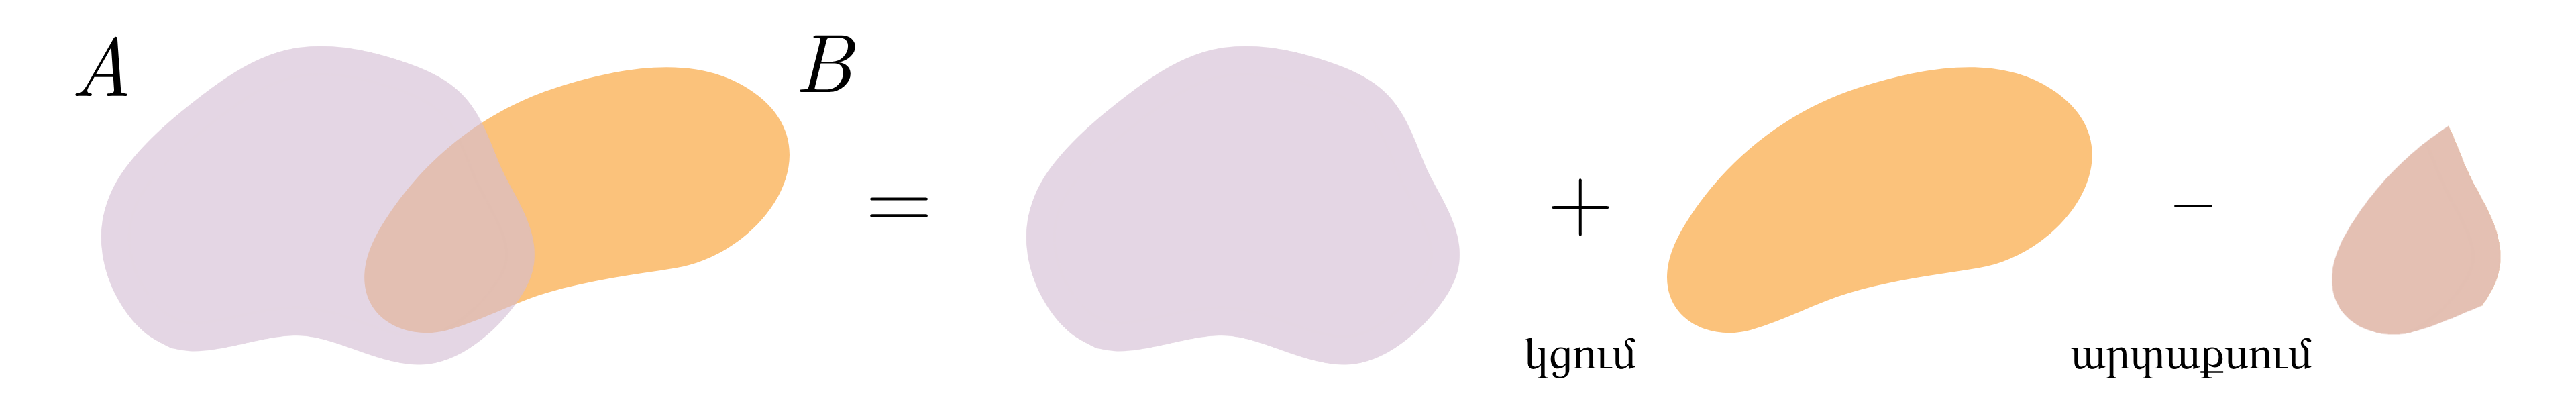
\includegraphics[width=\linewidth]{chapters/chapter 8/inclusion-exclusion.png}
\end{figure}

Մասնավորապես այս սկզբունքից հետևում է, որ 
\[
\PP[A \cup B] \le \PP[A] + \PP[B]
\]
ցանկացած $A$ և $B$ պատահույթների համար։ Ավելին, սա ճիշտ է ցանկացած թվով պատահույթների համար՝
\[
\PP\left[\bigcup_{n}A_n\right] \le \sum_n \PP[A_n]
\]
ընդ որում հավասարություն տեղի ունի միայն այն դեպքում, երբ $A_n$-երը ոչ մի ընդհանուր կետ չունեն։

\question{Կարո՞ղ եք դուրս բերել կցման-արտաքսման \href{https://www.youtube.com/shorts/xLQFOBo71w0}{սկզբունքը} երեք պատահույթների համար՝ $A$, $B$, $C$:}


\section{Պայմանական հավանականություն}

Ենթադրենք նետել ենք զառն, ու ընկել է ինչ-որ թիվ։

\newpage

\begin{description}
\item[Հարց 1․]  \textit{Որքա՞ն է հավանականությունը, որ ընկած թիվը զույգ է։}

\begin{marginfigure}
    \centering
    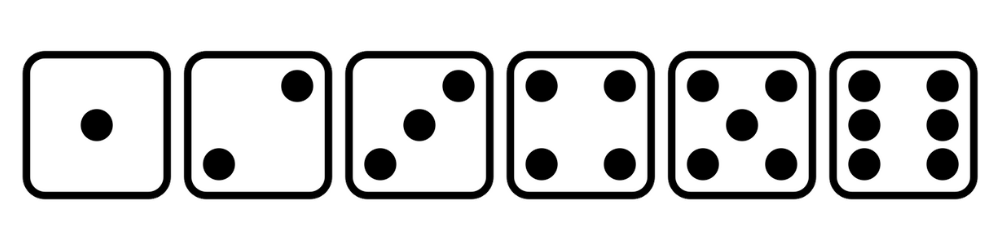
\includegraphics[width=\linewidth]{chapters/chapter 8/dice 1.png}
\end{marginfigure}

Դե քանի որ կա $6$ հնարավոր ելք, որոնցից ընդամենը $3$-ն են զույգ՝ $A = \{2, 4, 6\}$, հավանականությունը կլինի
\[
\PP[A] = \frac{3}{6} = \frac{1}{2}
\]

\item[Հարց 2․]  \textit{Որքա՞ն է հավանականությունը, որ ընկած թիվը զույգ է, եթե հայտնի է, որ այն պարզ է։}

\begin{marginfigure}
    \centering
    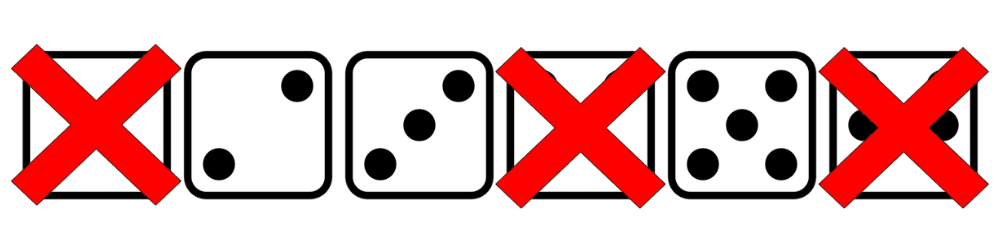
\includegraphics[width=\linewidth]{chapters/chapter 8/dice 2.png}
\end{marginfigure}

Եթե ինչ-որ կերպ գիտենք, որ զառի թիվը պարզ է, նշանակում է՝ այն չի կարող լինել $1$, $4$ կամ $6$։ Հետևաբար եթե այս երեքը ջնջենք ելքերի բազմությունից, տակը կմնա \textit{երեք} հնարավոր ելք՝ $B = \{2, 3, 5\}$։ Այս երեքից միայն մեկն է զույգ, հետևաբար հավանականությունը կլինի $\dfrac{1}{3}$:
\end{description}

Այսպիսով երկրորդ դեպքում, քանի որ կողքից հավելյալ տեղեկություն ունեինք, պատասխանը փոխվեց։ Պատճառն այն է, որ զառի թվի պարզ լինելու \textit{պայմանը} նշանակում է՝ հնարավոր են միայն այն ելքերը, որոնք պատկանում են $B$ բազմությանը։ Ուրեմն այդ \textit{պայմանի ներքո} մեզ մնում են միայն $A \cap B$ բազմության մեջ եղած՝ և՛ զույգ, և՛ պարզ ելքերը։

\begin{definition}
Երկու $A$ և $B$ պատահույթների համար\marginnote{եթե $\PP[B] \ne 0$}
\[
\PP[A \mid B] = \frac{\PP[A \cap B]}{\PP[B]}
\]
թիվը կանվանենք $A$-ի (պայմանական) \textbf{հավանականություն $B$ պայմանով։}
\end{definition}

Այլ կերպ ասած՝ եթե ունենք հավելյալ տեղեկություն/պայման, որ $B$ պատահույթը տեղի ունի, ապա փոխանակ նայենք, թե բոլոր $\Omega$ ելքերից որո՞նք են $A$-ի մեջ, $\Omega$-ն շպրտում ենք, վերցնում միայն $B$-ն, և նայում, թե $B$-ի տարրերից որո՞նք են $A$-ի մեջ։ 

\begin{figure}[h]
    \centering
    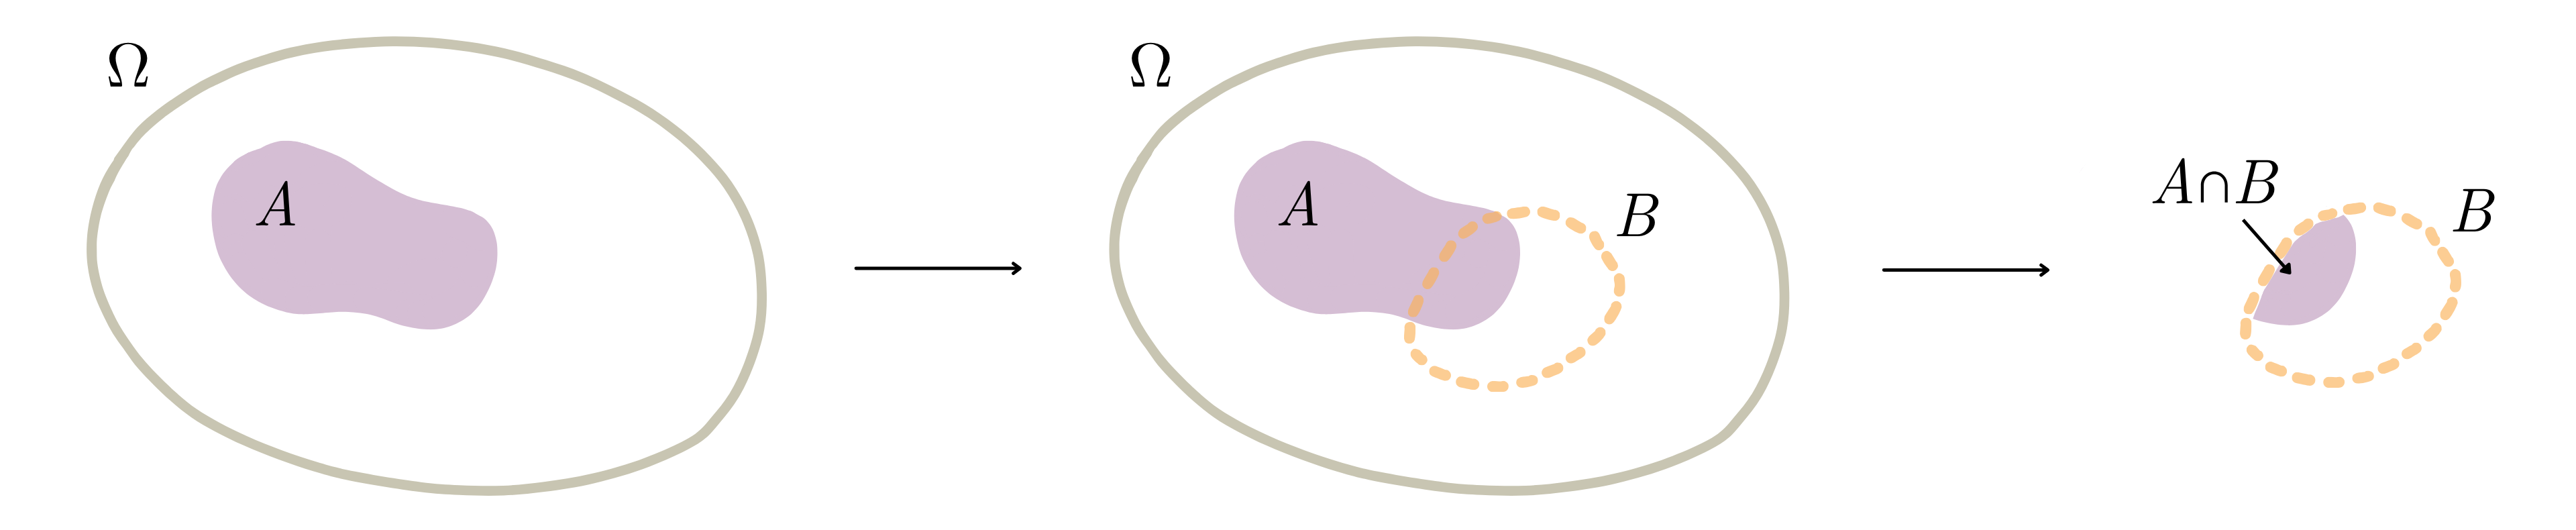
\includegraphics[width=\linewidth]{chapters/chapter 8/conditional.png}
\end{figure}

$\PP[A \mid B]$ թիվը ցույց է տալիս $A \cap B$-ի \textit{մասնաբաժինը} $B$-ի մեջ, այսինքն՝ $B$-ի որքա՞ն մասն\marginnote{քանի՞ տոկոսը} է կազմում $A$-ի հետ ունեցած հատումը։ 

Զառերի օրինակում՝
\[
\PP[\text{զույգ} \mid \text{պարզ է}]
= \PP[A \mid B]
= \frac{\PP[A \cap B]}{\PP[B]}
= \frac{\PP[\{2\}]}{\PP[\{2, 3, 5\}]}
= \frac{1/6}{3/6} = \frac{1}{3}
\]

\begin{example}
Նետել ենք երկու զառ։ Որքա՞ն է հավանականությունը, որ առաջին զառն ընկել է $2$, եթե զառերի գումարը $5$-ից մեծ չէ։

\newpage 

Առհասարակ հնարավոր է $36$ հատ ելք, որոնցից միայն $6$-ի դեպքում է առաջին զառն ընկնում $2$։ Բայց քանի որ \textit{գիտենք,} որ զառերի գումարը $5$ է, հնարավոր ելքերը լինում են ընդամենը $10$-ը․

\begin{center}
\begin{tabular}{c|*{6}{c}}
\toprule
& \dieimg{1} & \dieimg{2} & \dieimg{3} & \dieimg{4} & \dieimg{5} & \dieimg{6} \\
\midrule
\dieimg{1} & $\mathbf{2}$ & $\mathbf{3}$ & $\mathbf{4}$ & $\mathbf{5}$ & $6$ & $7$ \\
\dieimg{2} & $\mathbf{3}$ & $\mathbf{4}$ & $\mathbf{5}$ & $6$ & $7$ & $8$ \\
\dieimg{3} & $\mathbf{4}$ & $\mathbf{5}$ & $6$ & $7$ & $8$ & $9$ \\
\dieimg{4} & $\mathbf{5}$ & $6$ & $7$ & $8$ & $9$ & $10$ \\
\dieimg{5} & $6$ & $7$ & $8$ & $9$ & $10$ & $11$ \\
\dieimg{6} & $7$ & $8$ & $9$ & $10$ & $11$ & $12$ \\
\bottomrule
\end{tabular}
\end{center}

Այս $10$-ից միայն $3$-ի դեպքում է առաջին զառը ընկնում $2$, ուստի պատասխանն է $\dfrac{3}{10} = 0.3$:
\end{example}

\question{Որքա՞ն է հավանականությունը, որ Թբիլիսիում բնակվող պատա\-հական վերցված հայը խոսում է անգլերեն։}


\section{Բայեսի բանաձև}

Ենթադրենք $A$-ն ու $B$-ն զրոյից մեծ հավանականությամբ որևէ պատահույթներ են։ Եթե գիտենք $B$ պայմանի դեպքում $A$-ի տեղի ունենալու հավանականությունը, ինչպե՞ս ստանանք հակառակը՝ $A$ պայմանի դեպքում $B$-ի տեղի ունենալու հավանականությունը։

Գրենք $\PP[B \mid A]$-ի բանաձևը․
\[
\PP[B \mid A]
= \frac{\PP[B \cap A]}{\PP[A]}
= \frac{\PP[A \cap B]}{\PP[A]}
= \frac{\PP[A \mid B] \cdot \PP[B]}{\PP[A]}
\]
Հիասքանչ․ \marginnote{\href{https://upload.wikimedia.org/wikipedia/commons/c/c9/Bayes_theorem_visual_proof.svg}{պատկերավոր ապացույց}} $A$-ի ու $B$-ի տեղերը փոխվեցին։ Ստացվեց, որ ${\PP[B \mid A]}$-ն արտահայտեցինք ${\PP[A \mid B]}$-ով։ Այս արդյունքը կոչվում է \textit{Բայեսի բանաձև։}

\begin{example}
Բնության մեջ հրդեհներ տեղի են ունենում հազարից մեկ, ենթադրենք՝ $0.01$ հավանականությամբ, ընդ որում դրանցից $90\%$-ում առաջանում է տեսանելի ծուխ։ Մյուս կողմից՝ խորոված անելիս նույնպես ծուխ է առաջանում, և օրը ցերեկով ծուխ տեսնելու հավանականությունը այնքան էլ ցածր չէ, ասենք՝ $10\%$։ 

Նայում եք հեռուն և տեսնում ծուխ։ Որքա՞ն է հավանականությունը, որ Ձեր տեսածը հրդեհ է։
Նախ եթե $F$-ով նշանակենք հրդեհ, իսկ $S$-ով՝ ծուխ լինելու հավանականությունը, կունենանք՝
\[
\PP[F] = 0.01, \qquad \PP[S] = 0.1
\]
և $\PP[S \mid F] = 0.9$: Ուրեմն ըստ Բայեսի բանաձևի՝
\[
\PP[F \mid S] = \frac{\PP[S \mid F] \cdot \PP[F]}{\PP[S]} = \frac{0.01 \cdot 0.9}{0.1} = 0.09
\]
Անհանգստանալու կարիք չկա․ ամենայն հավանականությամբ ծուխը խորովածից է։
\end{example}


Քննարկենք ևս մի հետաքրքիր խնդիր։ Պատկերացրեք՝ ունենք մի համալսարան, որտեղ
\begin{itemize}
    \item կանանց $10\%$-ն է ձախլիկ
    \item տղամարդկանց $15\%$-ն է ձախլիկ
    \item ուսանողների $\dfrac{3}{5}$-ը կին են, մյուսները՝ տղամարդ
\end{itemize}

Որքա՞ն է հավանականությունը, որ պատահական վերցված ուսանողը կլինի ձախլիկ։

% \begin{figure}[h]
%     \centering
%     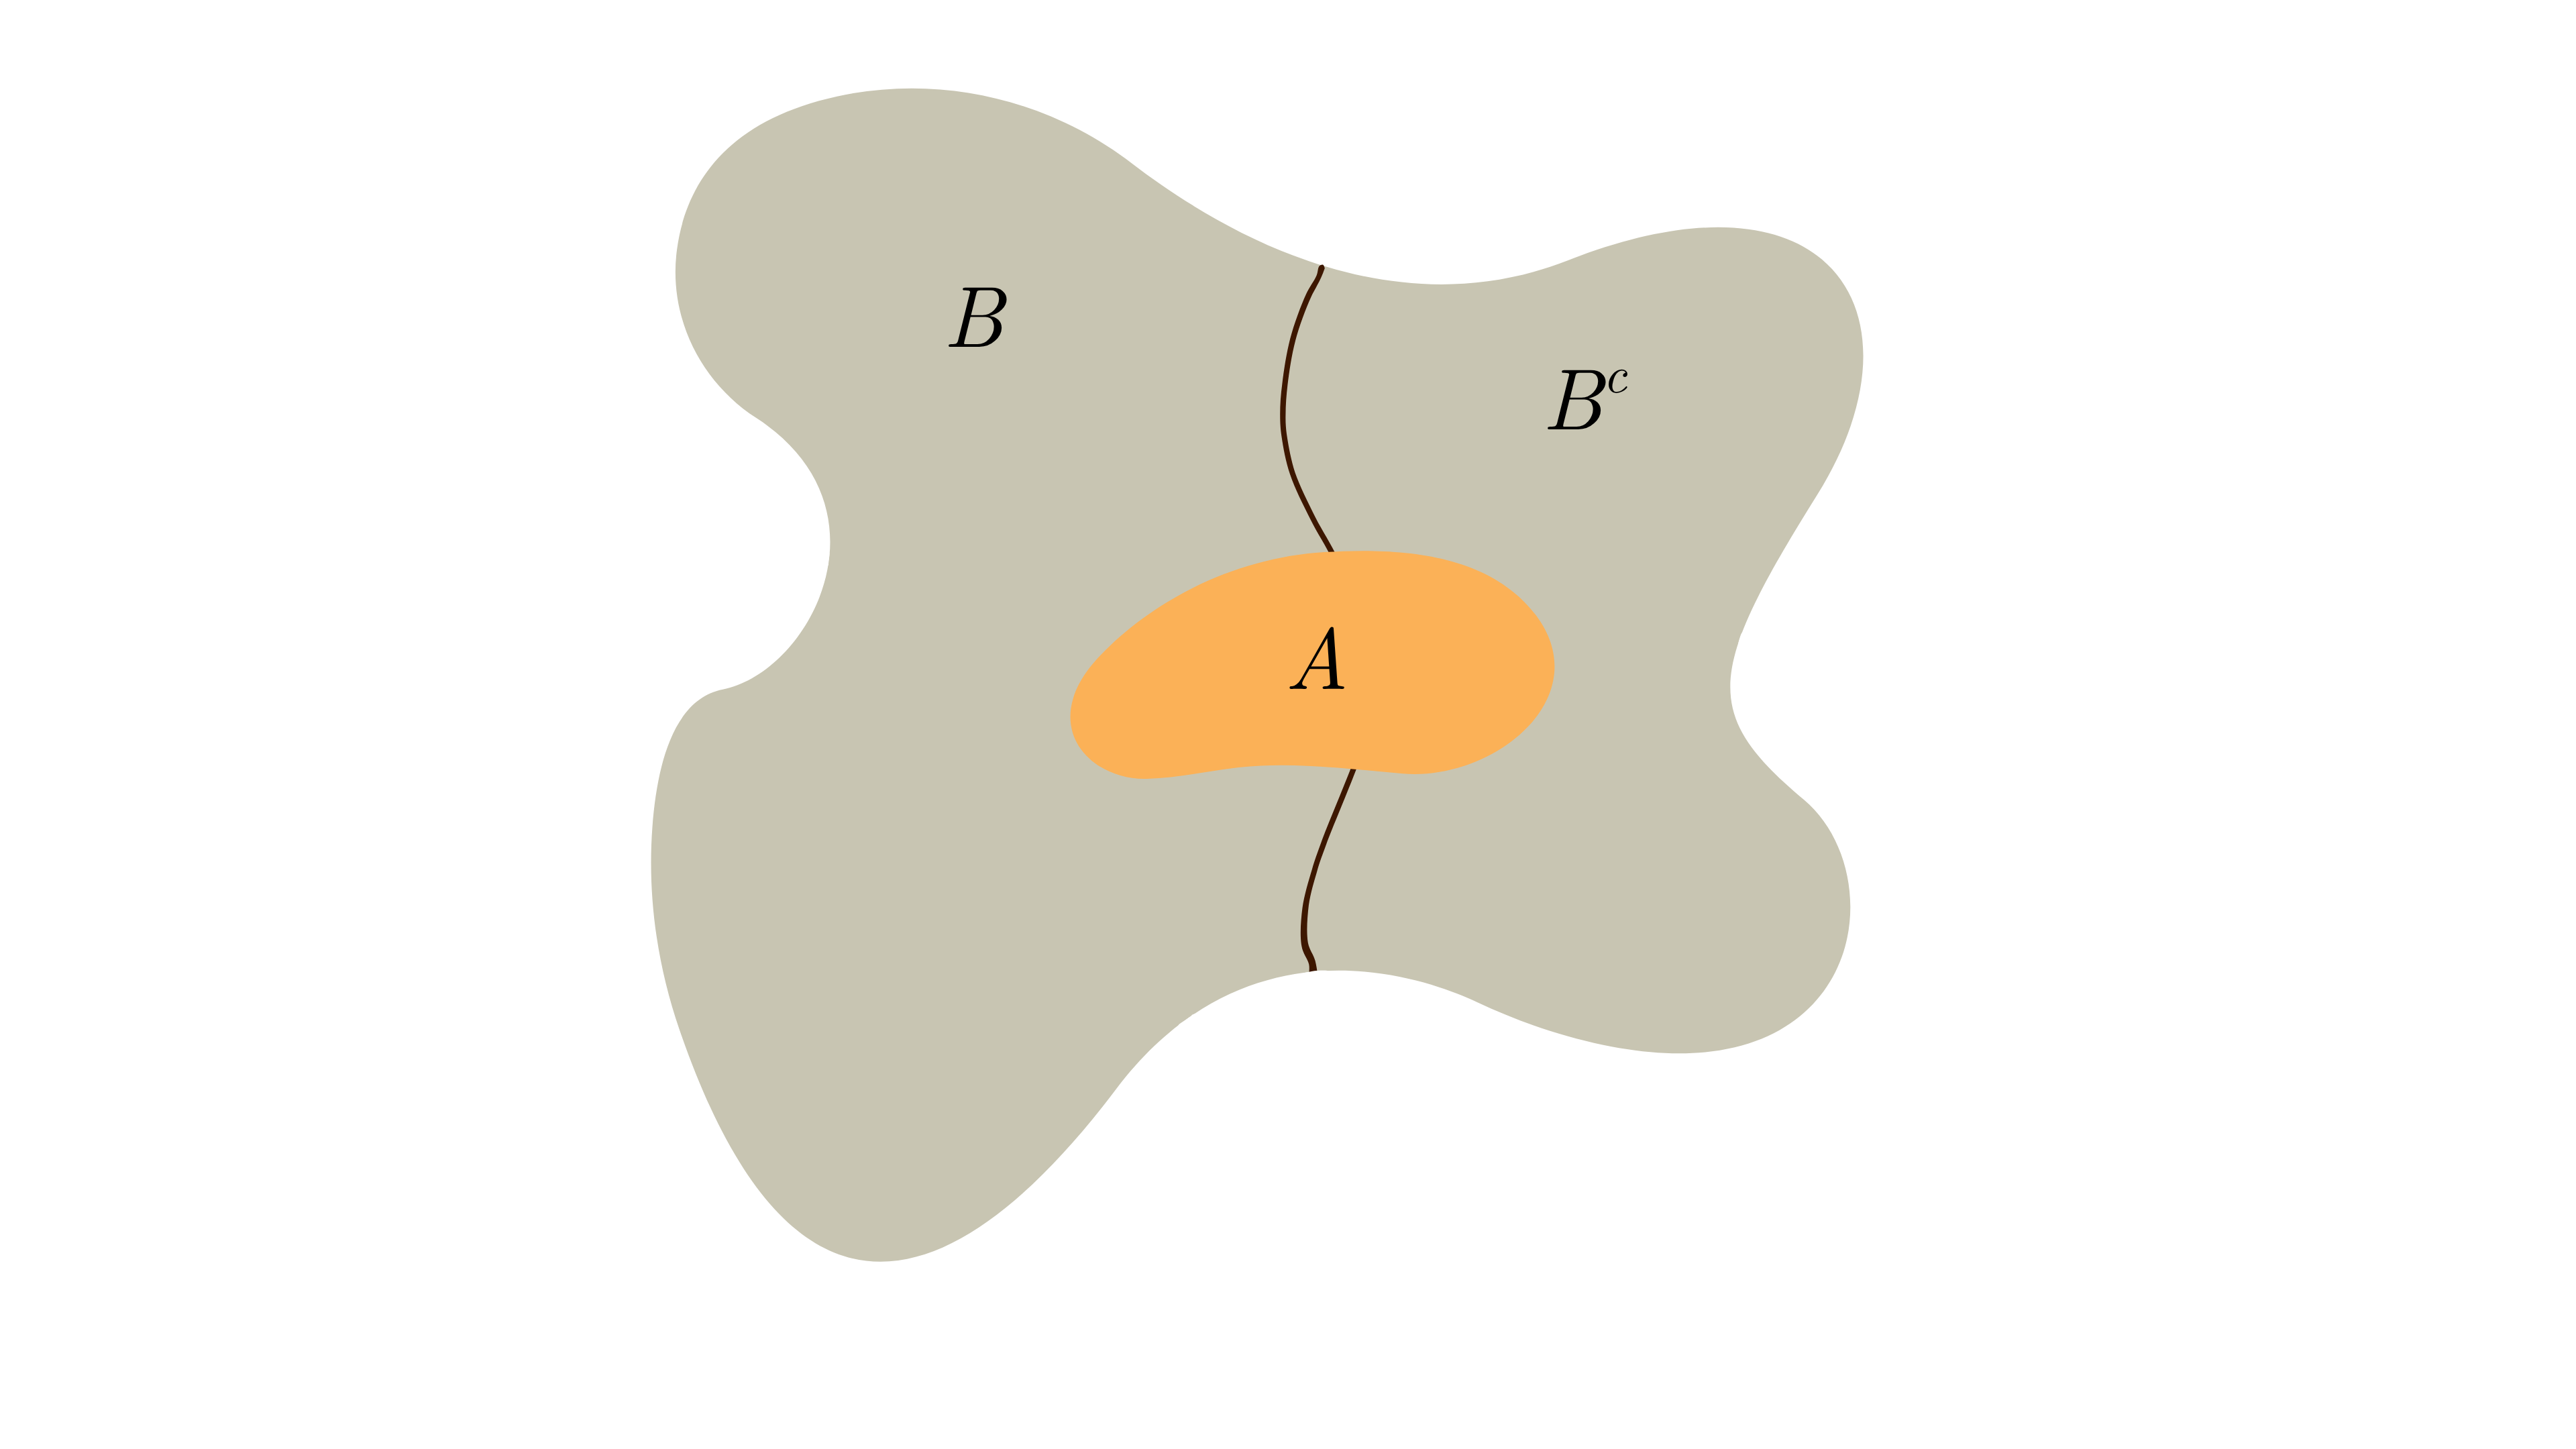
\includegraphics[width=0.7\linewidth]{chapters/chapter 8/total probability 1.png}
% \end{figure}

Նախ $A$-ով նշանակենք կին լինելու պատահույթը,\marginnote[*+1]{$B^c$-ն կլինի տղամարդ լինելունը} իսկ $B$-ով՝ ձախլիկ լինելունը։ Այդ դեպքում ձախլիկներին կարող ենք բաժանել երկու չհատվող մասերի՝
\[
\big\{\text{ձախլիկներ}\big\}
\; = \;  \big\{\text{կին ձախլիկներ}\big\} \; \cup  \; \big\{\text{տղամարդ ձախլիկներ}\big\}
\]
կամ որ նույնն է՝
\[
\PP[A] = \PP[A \cap B] + \PP[A \cap B^c]
\]
\begin{figure}[h]
    \centering
    \subfloat{{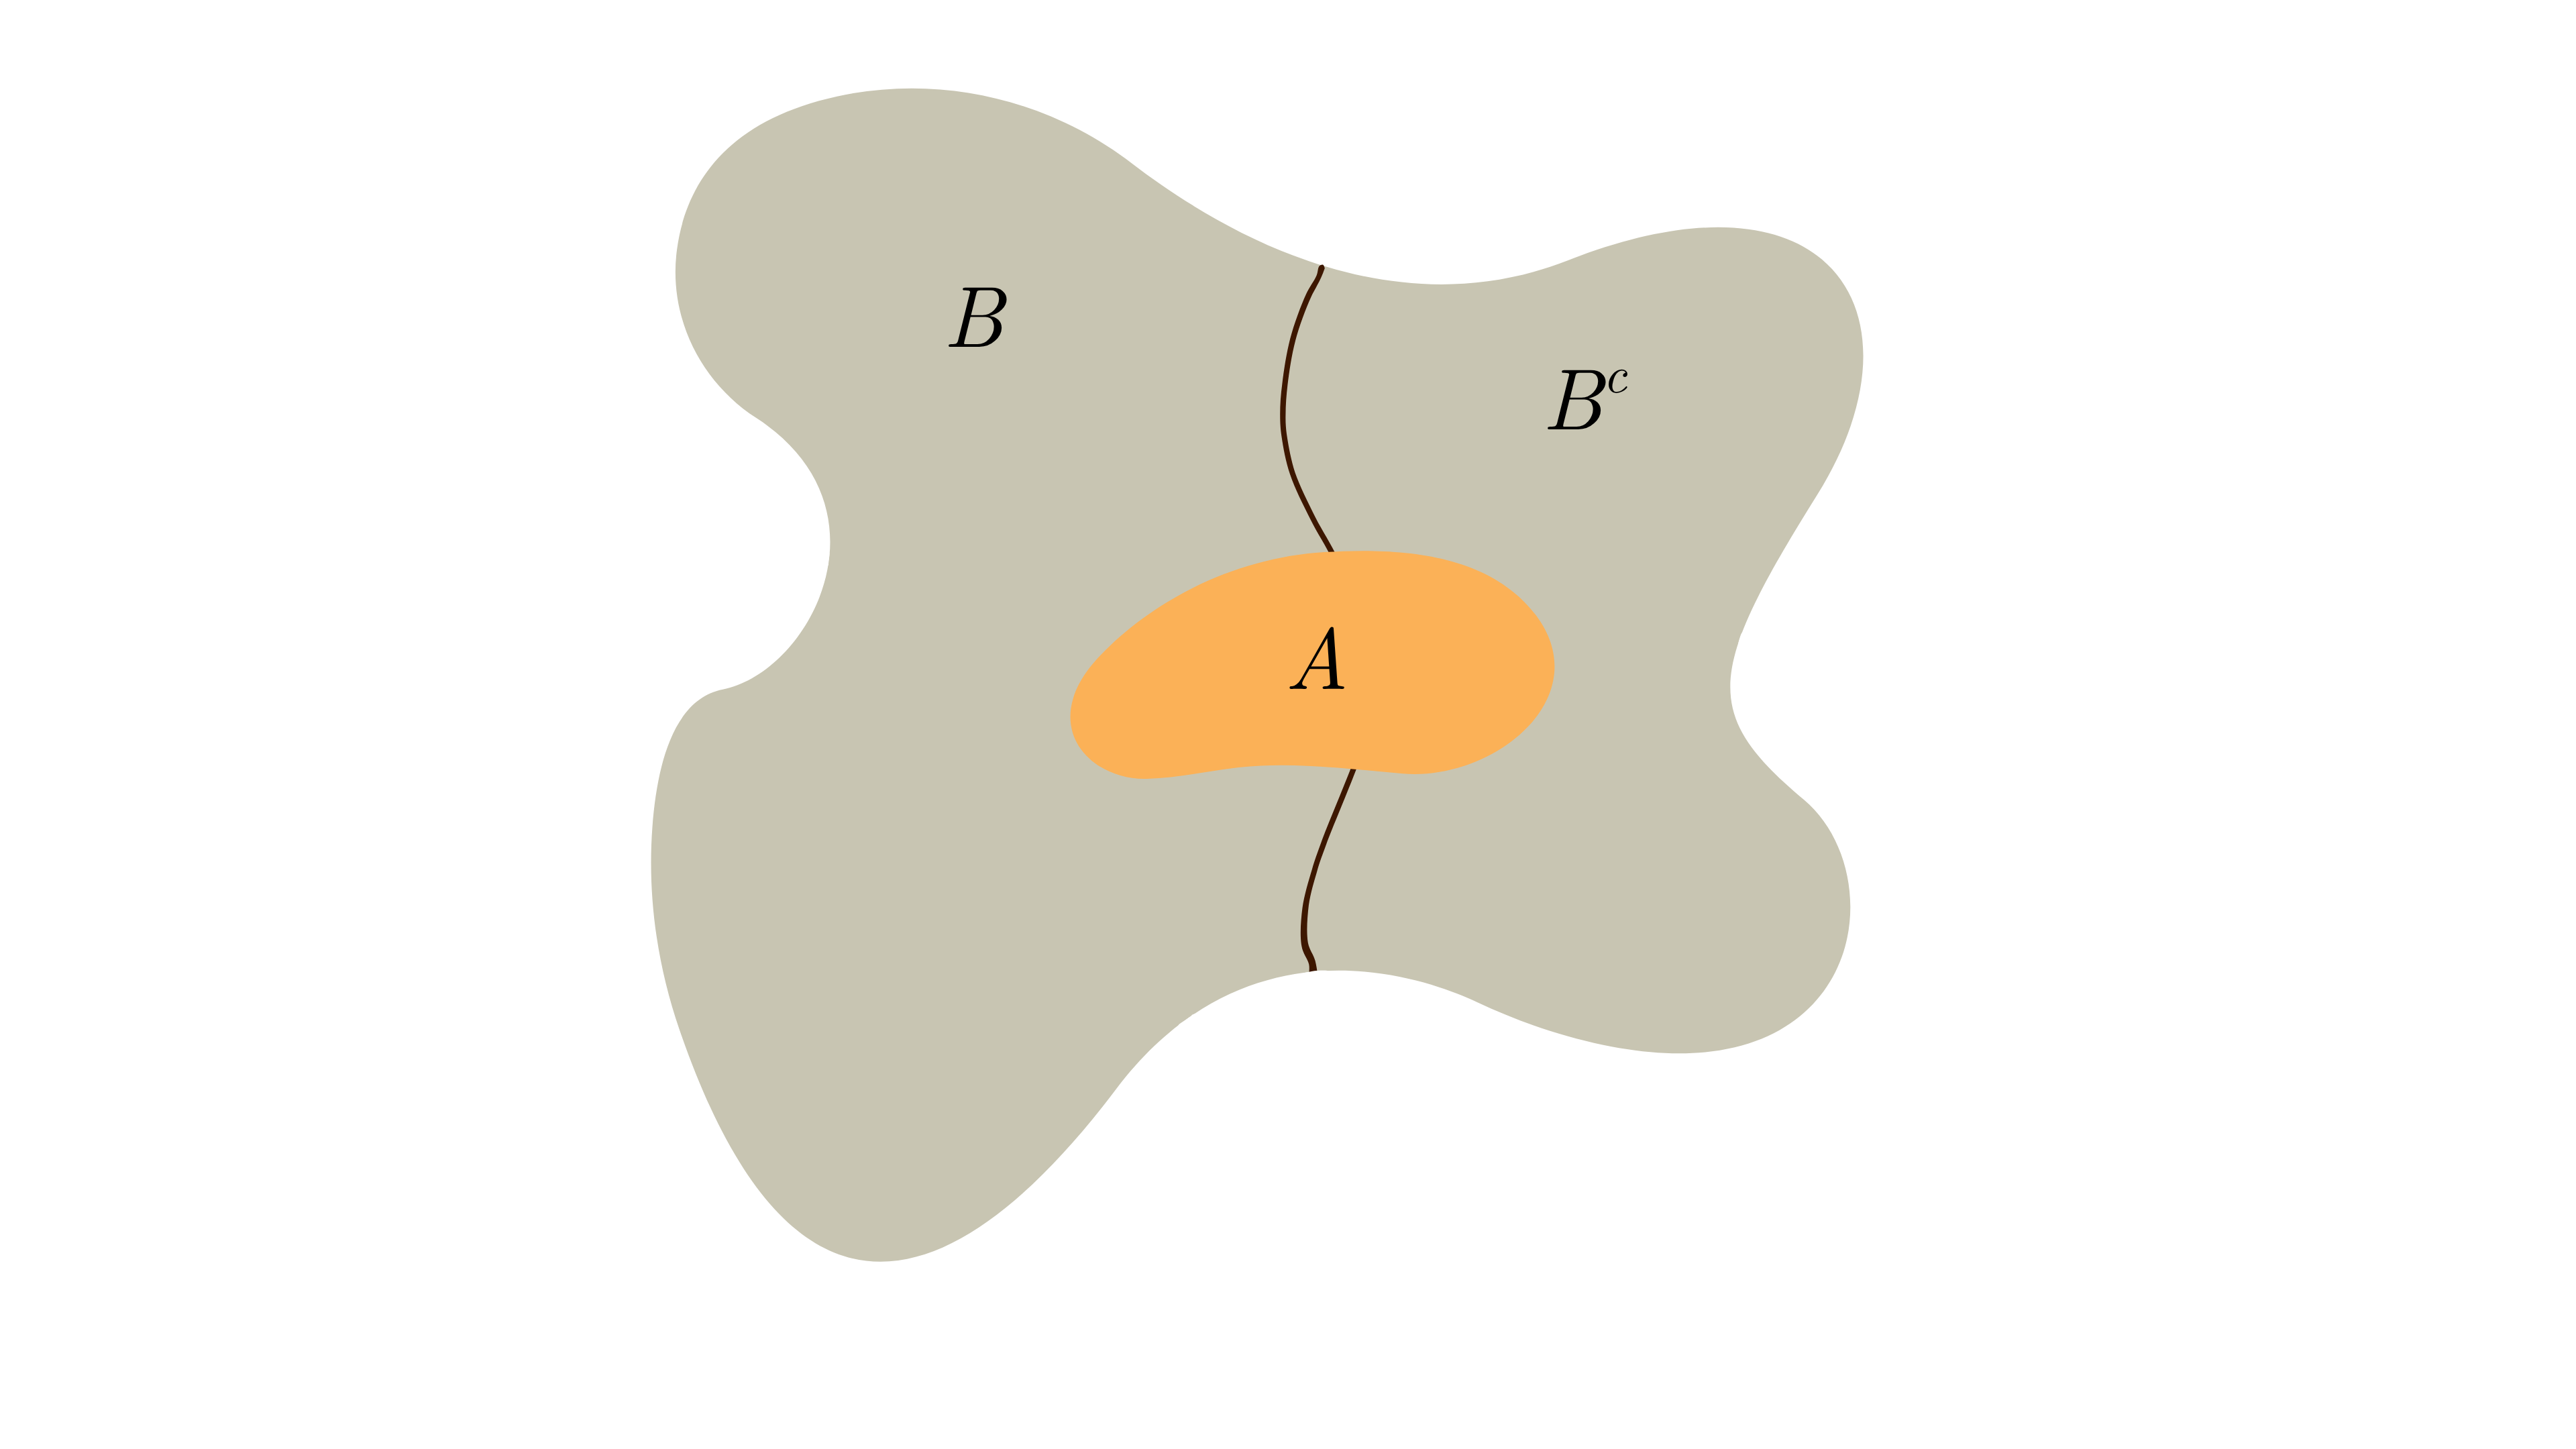
\includegraphics[trim={13cm 0 13cm 0},clip,width=0.5\linewidth]{chapters/chapter 8/total probability 1.png} }}%
    % \qquad
    \subfloat{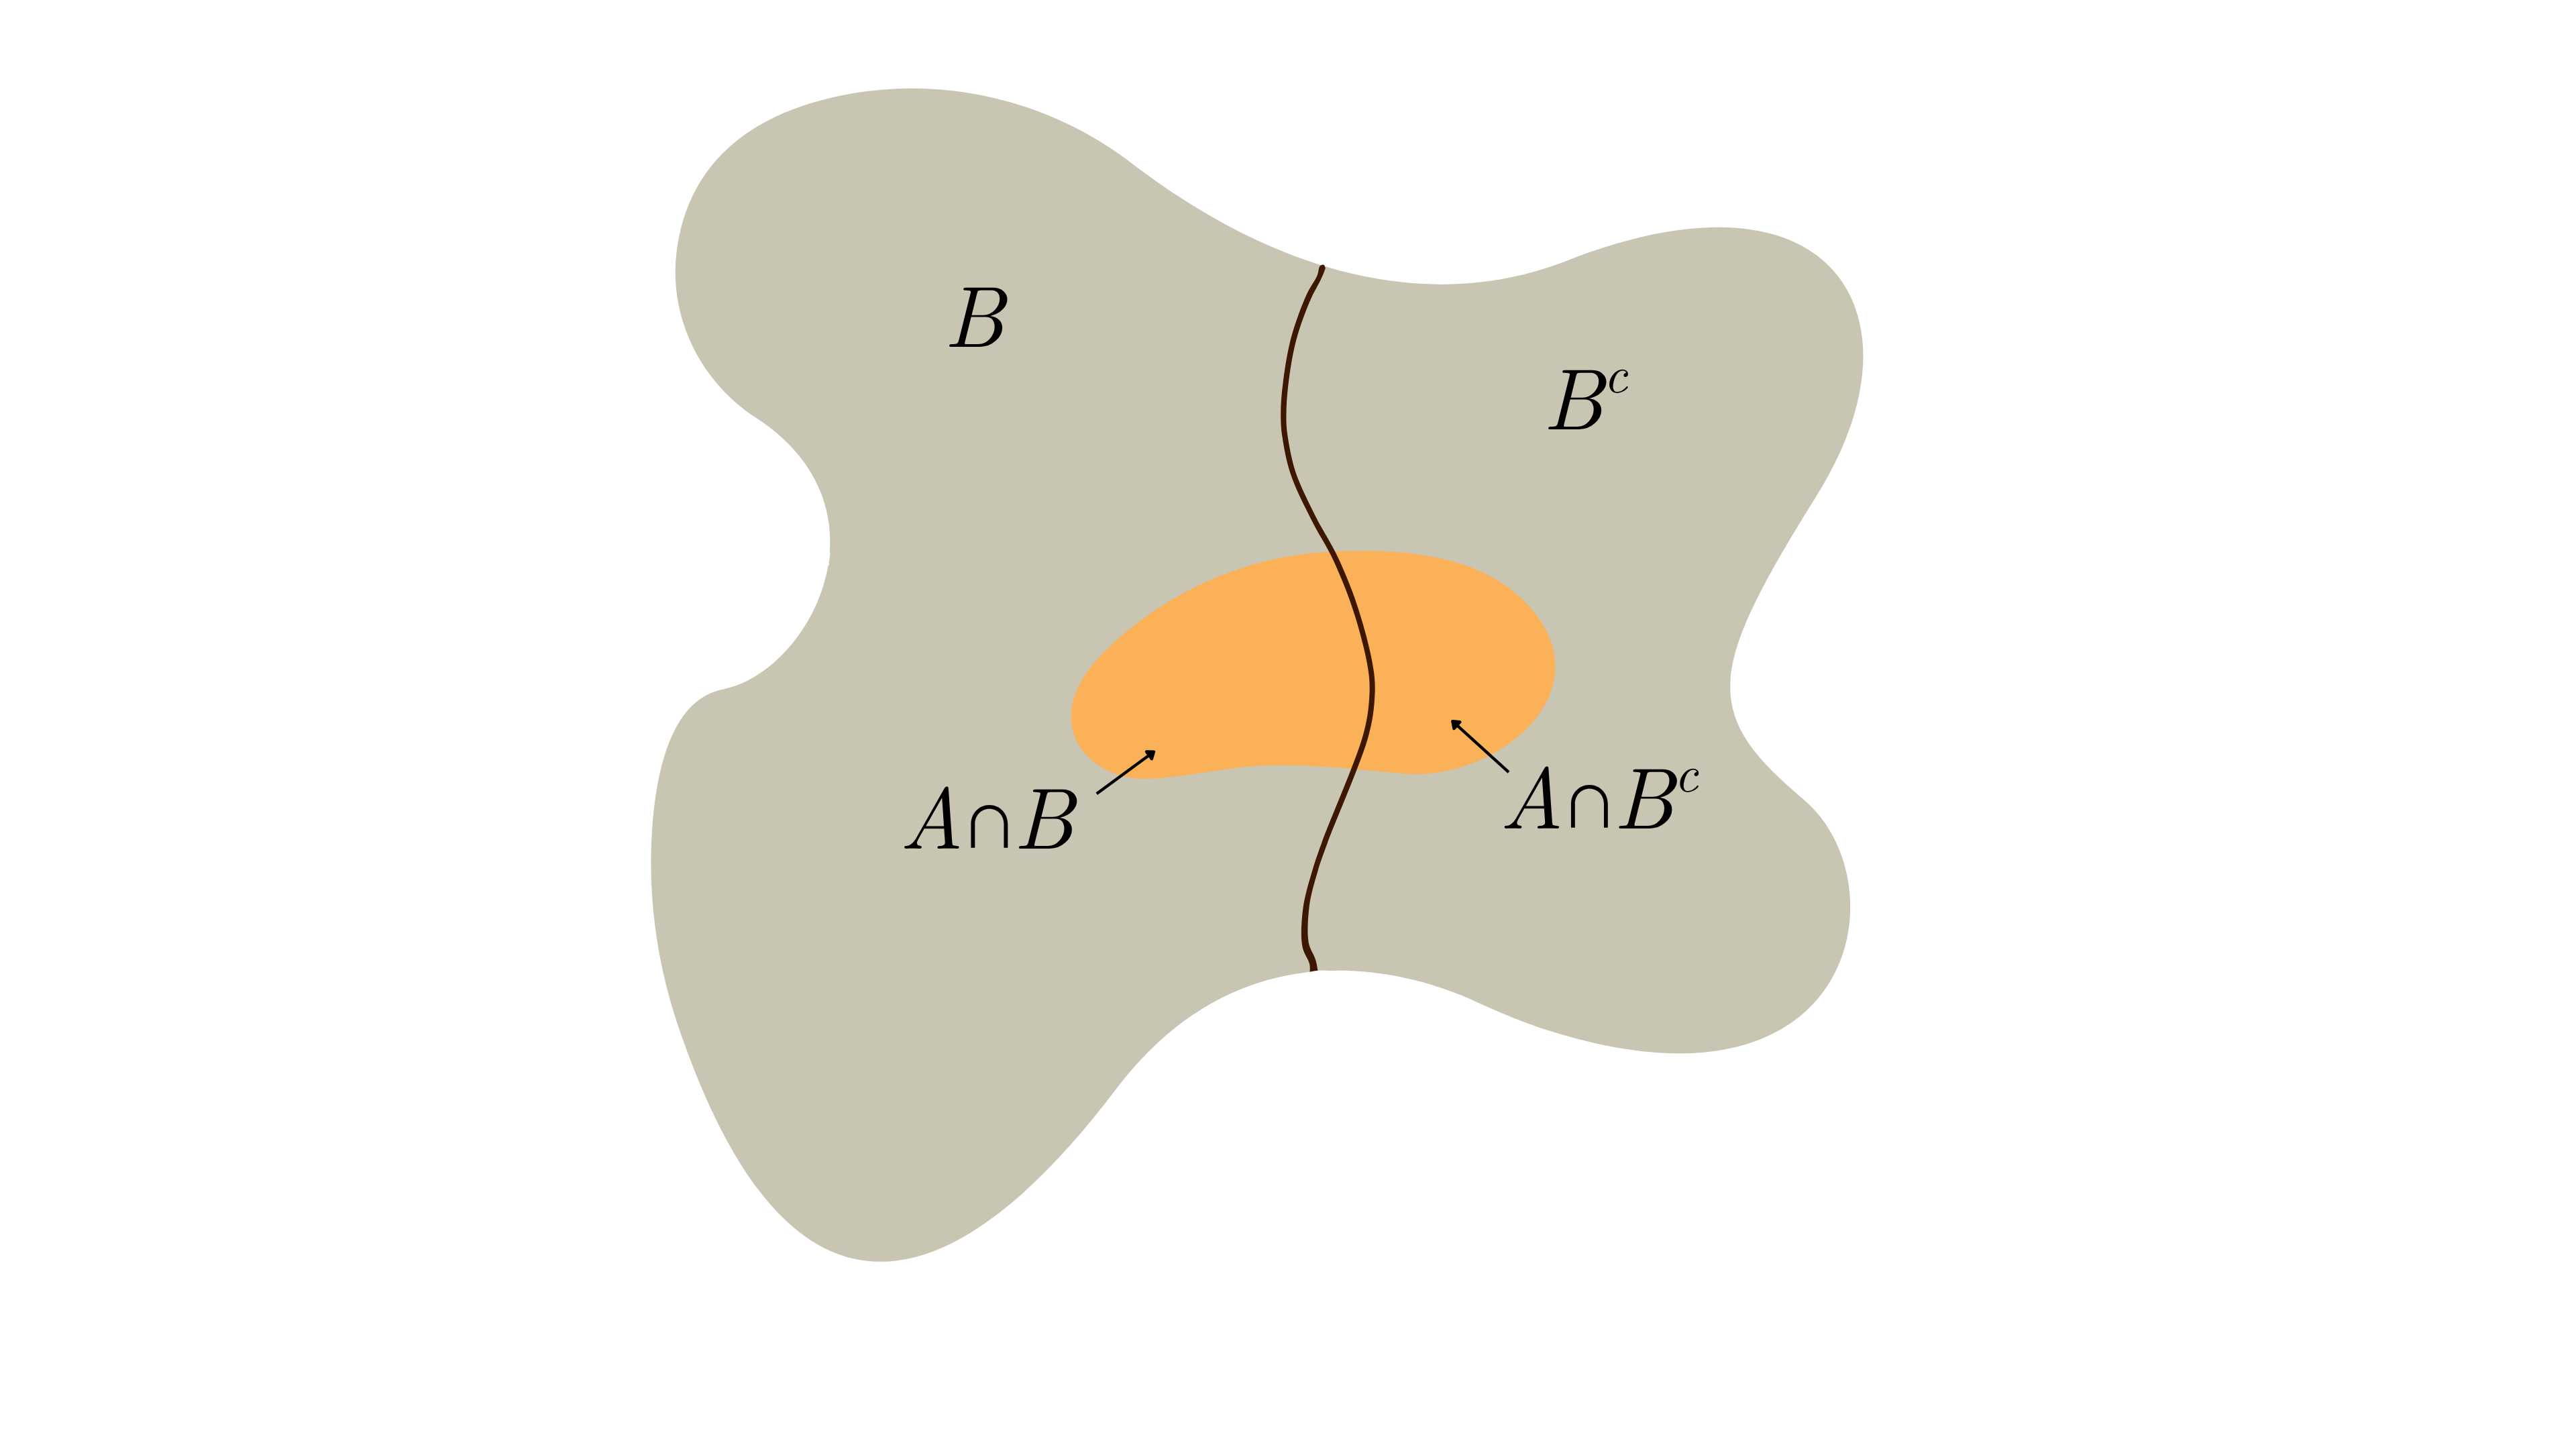
\includegraphics[trim={13cm 0 13cm 0},clip,width=0.5\linewidth]{chapters/chapter 8/total probability 2.png}} %
\end{figure}

Այստեղ արդեն օգտվելով պայմանական հավանականությունից՝
\begin{align*}
\PP[A] &= \PP[A \cap B] + \PP[A \cap B^c]
\\&= \PP[B] \cdot \PP[A \mid B] + \PP[B^c] \cdot \PP[A \mid B^c]
\\&= \frac{3}{5} \cdot 0.1 + \frac{2}{5} \cdot 0.15 = \frac{3}{25} = 0.12
\end{align*}
և խնդիրը լուծված է։ Ստացվածը կոչվում է \textit{լրիվ հավանականության բանաձև․}
\[
\PP[A] = \PP[B] \cdot \PP[A \mid B] + \PP[B^c] \cdot \PP[A \mid B^c]
\]
Ինչո՞ւ «լրիվ»։ Որովհետև կարծես բոլոր դեպքերը բաժանում ենք երկու ենթադեպքերի, յուրաքանչյուրում հաշվում, ապա համապատասխան կշիռներով\marginnote{ըստ էության՝ ենթադեպքերի գծային զուգակցությունն է} (դեպքերի հավանականություններով) բազմապատկելով ու գումարելով ստանում լրիվ հավանականությունը։

Անշուշտ, նույնը ճիշտ է նաև, եթե բաժանենք ոչ թե երկու, այլ երեք և ավելի չհատվող ենթադեպքերի․\begin{marginfigure}[*-2]
    \centering
    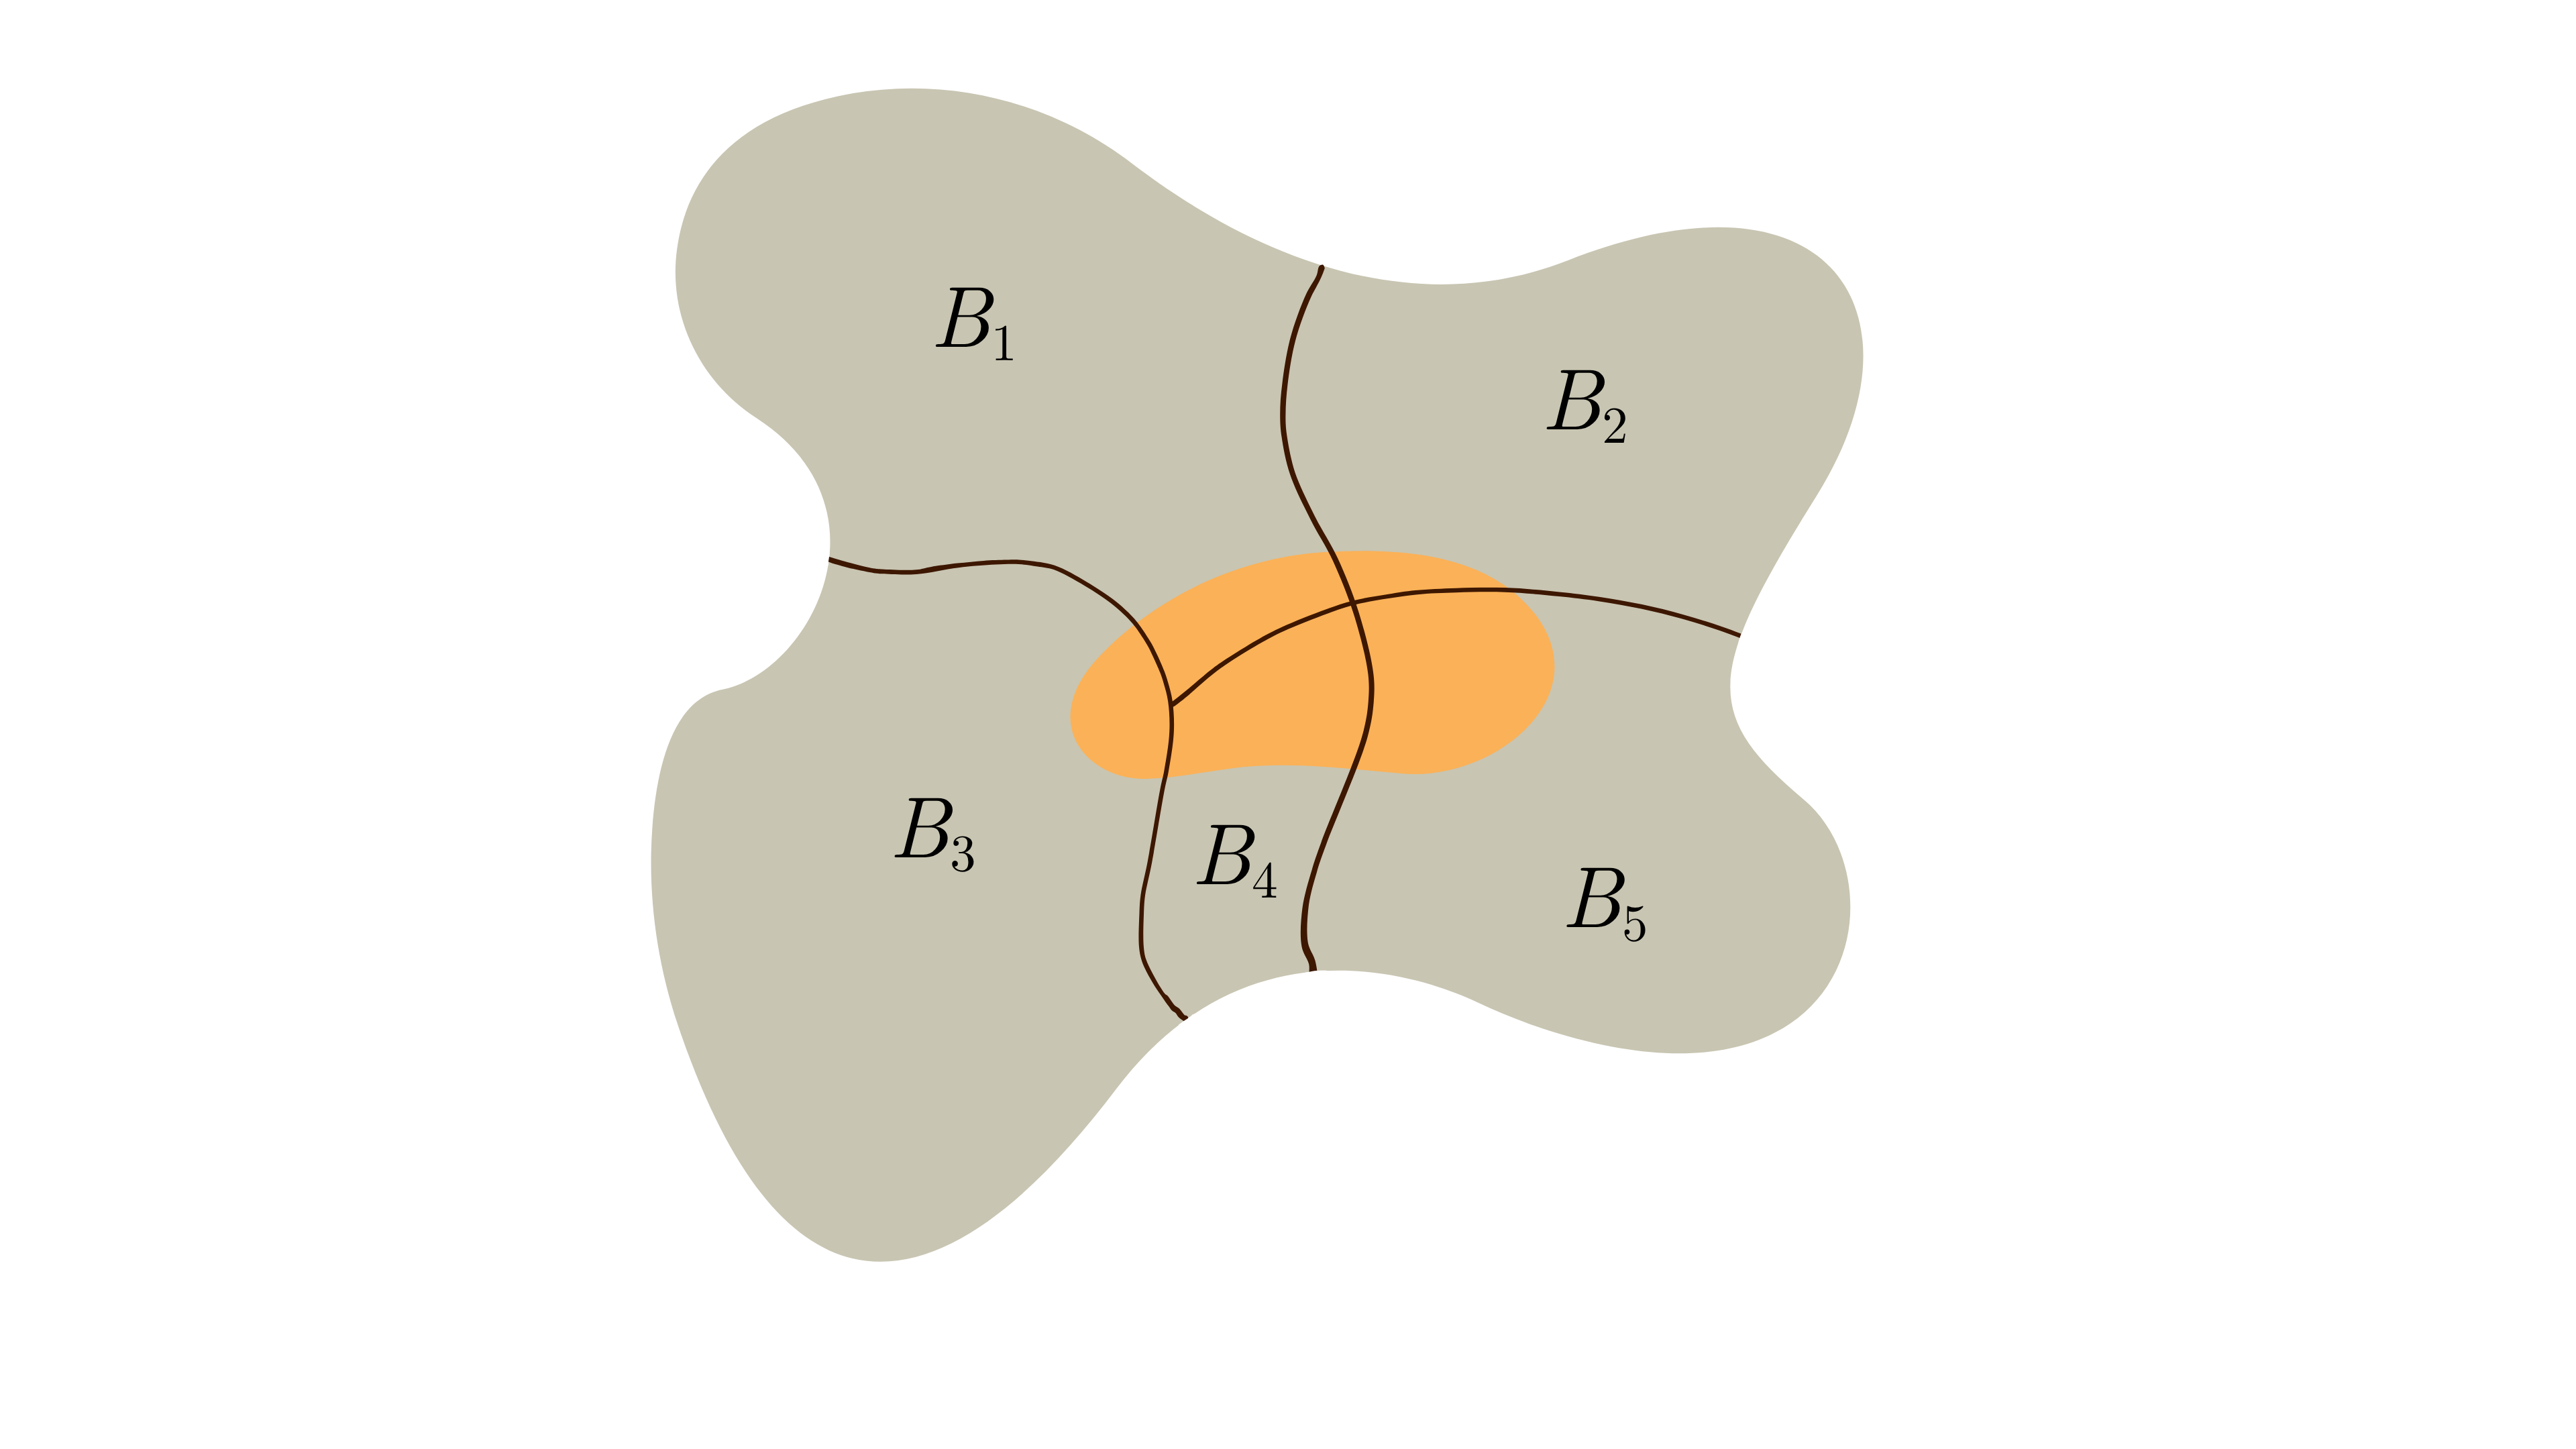
\includegraphics[trim={15cm 0 15cm 0},clip,width=\linewidth]{chapters/chapter 8/total probability generalized.png}
\end{marginfigure}
\begin{theorem}
Եթե $A$ պատահույթը կարելի է բաժանել մի քանի չհատվող պատահույթների միջև՝ $A \subset B_1 \cup B_2 \cup \dots$, ապա
\[
\PP[A] = \PP[B_1] \cdot \PP[A \mid B_1] + \PP[B_2] \cdot \PP[A \mid B_2] + \dots
\]
\end{theorem}

\warning{Բանաձևը ճիշտ է, միայն եթե $B_n$-երը \textbf{չեն հատվում։}}

\begin{example}
Ունենք $52$ խաղաթուղթ։ Պատահականորեն վերցնում ենք դրանցից մեկը, տակը մնում է $51$ հատ։ Որքա՞ն է հավանականու\-թյունը, որ եթե վերցնենք ևս մեկ խաղաթուղթ, այն կլինի սիրտ։\marginnote{սրտերը $13$ հատ են}

Նշանակենք՝
\begin{align*}
    A &= \text{երկրորդ հանածը սիրտ է} \\
    B &= \text{առաջին հանածը սիրտ է}
\end{align*}

\begin{marginfigure}
\resizebox{0.9\linewidth}{!}{%
\begin{tikzpicture}[scale=1]
% 1st level
\draw[very thick, blue]%
   (0,0) 
   -- node[above, sloped, align=center]
      {\textcolor{black}{$1$-ինը $\heartsuit$ է}\\$(1/4=25\%)$} 
   (\wideOne,\distOne);
\draw[very thick, blue] 
   (0,0) 
   -- node[below, sloped, align=center]
      {\textcolor{black}{$1$-ինը $\heartsuit$ չէ}\\($3/4=75\%$)} 
   (\wideOne,-\distOne);

% 2nd, 3rd and 4th Level
\draw[very thick, blue] 
   (\wideOne,\distOne)
   -- node[above, align=center, sloped]
      {\textcolor{black}{$2$-րդը $\heartsuit$ է}\\$(12/51=23.53\%)$}
   ++ (\wideTwo,\distTwo) 
   ; 
\draw[thick] 
   (\wideOne,\distOne) 
   -- node[below, align=center, sloped]
      {$2$-րդը $\heartsuit$ չէ}
   ++ (\wideTwo,-\distTwo) 
   ;
\draw[very thick, blue] 
   (\wideOne,-\distOne) 
   -- node[above, align=center, sloped]
      {\textcolor{black}{$2$-րդը $\heartsuit$ է}\\$(13/51=25.49\%)$}
   ++ (\wideTwo,\distTwo) 
   ;  
\draw[thick] 
   (\wideOne,-\distOne)
   -- node[below, align=center, sloped]
      {$2$-րդը $\heartsuit$ չէ}
   ++ (\wideTwo,-\distTwo) 
   ; 
\end{tikzpicture}
}
\end{marginfigure}
Առաջին խաղաթուղթը հանելուց հետո
\begin{itemize}
    \item եթե հանվածը սիրտ է, ապա մնում է ևս $12$ սիրտ
    \item եթե հանվածը սիրտ չէ, ապա մնում է $13$ սիրտ
\end{itemize}
այսինքն՝ $\PP[A \mid B] = \dfrac{12}{51}$ և $\PP[A \mid B^c] = \dfrac{13}{51}$:

Մյուս կողմից $\PP[B] = \dfrac{13}{52}$, հետևաբար լրիվ հավանականությունն է՝
\[ 
\PP[A] =
\PP[B]\cdot \PP[A\mid B] + \PP[B^c] \cdot \PP[A \mid B^c] =
\frac{13}{52}\cdot \frac{12}{51} + \frac{39}{52}\cdot \frac{13}{51} = \frac{1}{4}
\]
Կարո՞ղ էիք պատասխանը ստանալ այլ եղանակով։
\end{example}


\section{Անկախություն}

Վերևում հաշվեցինք զառը կամ մետաղադրամը նետելիս ստացվող տարբեր պատահույթների հավանականություններ։ Իսկ ի՞նչ, եթե կա\-տա\-րենք այսպիսի փորձ․ միաժամանակ նետենք զառը և մետաղադրամը։ Որևէ ազդեցություն կունենա՞ արդյոք զառի ընկած թիվը մետաղադրամի արդյունքի վրա։ Կփոխվի՞, ասենք, զառի $3$ ընկնելու հավանականու\-թյու\-նը, եթե իմանաք, որ մետաղադրամը գիր է ընկել։ Իհարկե ոչ․ զառը նույն\-իսկ տեղյակ չէ, որ Դուք իրենից բացի մետաղադրամ եք նետել, և դրան\-ցից մեկը մյուսի վրա ոչ մի ազդեցություն չունի։

Նույն կերպ իրարից կախում չունեն 
\begin{itemize}
    \item մետաղադրամների երկու տարբեր նետումները
    \item իրար հետևից կամ թեկուզ միաժամանակ նետված երկու զառերը
    \item միևնույն զառի առաջին և երկրորդ նետումները
    \item պատահական վերցված երկու մարդկանց հասակները
\end{itemize}
և այլն։ Այլ կերպ ասած՝ դրանք անկախ են։

\begin{definition}
Կասենք, որ $A$ և $B$ պատահույթներն \textbf{անկախ} են, եթե 
\[
\PP[A \cap B] = \PP[A] \cdot \PP[B]
\]
կամ համարժեքորեն՝\marginnote{երկու կողմը բաժանենք $\PP[B]$-ի}
\[
\PP[A \mid B] = \PP[A]
\]
\end{definition}

Երկրորդ պայմանը նշանակում է, որ $A$ պատահույթի համար $B$-ն եղած-չեղած մի հաշիվ է․ $A$-ի հավանականությունը $B$ պայմանի դեպքում նույնն է, ինչ առանց $B$ պայմանի։  

\begin{example}
Վերջին անգամ նետենք երկու զառ։ Նշանակենք՝
\begin{align*}
    A &= \text{առաջին զառը զույգ է} \\
    B &= \text{երկրորդ զառը կենտ է}
\end{align*}
Պարզենք, թե որքան է $A \cap B$ պատահույթի հավանականությունը։

Նախ $\PP[A] = \PP[B] = \dfrac{3}{6} = 0.5$։ Քանի որ զառերի ելքերն իրարից անկախ են, ապա հավանականությունը, որ միաժամանակ առաջին զառը կլինի զույգ, իսկ երկրորդը՝ կենտ, հավասար է
\[
\PP[A \cap B] = \PP[A] \cdot \PP[B] = \frac{1}{2} \cdot \frac{1}{2} = 0.25
\]
% առանց ավելորդ հաշվարկների։
\end{example}

\question{Նետում ենք $100$ զառ։ Որքա՞ն է հավանական, որ բոլորը կընկնեն զույգ։ Իսկ որ գոնե մեկը կընկնի կե՞նտ։}

\begin{example}
Մոտենում եք երկու պատահական անցորդի, հարցնում, թե նրանք որ ամսին են ծնվել, և եթե այն համընկնում է Ձեր ծնված ամսվա հետ, ապա ուրախանում եք։ Որքա՞ն է հավանական, որ երկու հոգուց գոնե մեկի ամիսը կհամընկնի Ձերինի հետ։

Եթե $A_1$-ով նշանակենք առաջին, իսկ $A_2$-ով՝ երկրորդ անցորդի ծննդյան ամսվա համընկնելը Ձեր ամսվա հետ, ապա
\begin{itemize}
    \item $A_1$-ն ու $A_2$-ը կլինեն անկախ
    \item ընդ որում $\PP[A_1] = \dfrac{1}{12}$ և $\PP[A_2] = \dfrac{1}{12}$ 
\end{itemize}

Մեր նպատակն է հաշվել $A_1$-ից ու $A_2$-ից գոնե մեկի տեղի ունենալու հավանականությունը, հետևաբար՝
\begin{align*}
\PP[A_1 \cup A_2] &= \PP[A_1] + \PP[A_2] - \PP[A_1 \cap A_2] \\&= \PP[A_1] + \PP[A_2] - \PP[A_1] \cdot \PP[A_2] \\&= \frac{1}{12} + \frac{1}{12} - \frac{1}{12^2} = \frac{23}{144} \approx 0.16
\end{align*}
\end{example}

Նկատենք նաև, որ եթե երկու $A$ ու $B$ պատահույթներ անկախ են, \marginnote{ասենք $1$-ին զառի զույգ լինելն ու $2$-րդի կենտ լինելը} ապա նրանց լրացումները`
\begin{itemize}
    \item $A^c$-ն ու $B$-ն
    \item $A^c$-ն ու $B^c$-ն
    \item $A$-ն ու $B^c$-ն
\end{itemize}
նույնպես անկախ են։ Այսինքն եթե $A$-ի տեղի ունենալը չի ազդում $B$-ի հավանականության վրա, ապա բնականաբար $A$-ի տեղի չունենալը նույնպես չի ազդում $B$-ի վրա։

Նման ձևով, եթե մի պատահույթի տեղի ունենալուց հետևում է, որ մյուսը չի կարող տեղի ունենալ (այսինքն դրանք չեն հատվում՝ անհամատեղելի են), ապա այդ երկուսի միջև ինչ-որ կապ կա, և դրանք անկախ չեն։ Հետևաբար,
\begin{theorem}
Եթե $A$ և $B$ պատահույթներն անկախ են\marginnote{և եթե $\PP[A]$, $\PP[B]$ $\ne 0$}, ապա նրանք չեն կարող անհամատեղելի լինել։
\end{theorem}

\question{Կարո՞ղ եք ապացուցել թեորեմը։}


\section{Երկրաչափական հավանականություն}

Հավանականային խնդիրները լուծելու ամենահաճելի ձևերից է դրանց երկրաչափորեն մոտենալը։

\question{$AD$ հատվածից պատահականորեն վերցնում ենք որևէ կետ։ Ի՞նչ եք կարծում, որքան է հավանական, որ այն կգտնվի $B$ և $C$ կետերի միջև։}
\begin{figure}[h]
\centering
\begin{tikzpicture}[scale=0.65]
  \draw[<->, myblue] (-6.5,0) -- (6.5,0);
  \foreach \x in {-6,...,6} {
    \draw (\x,0.1) -- (\x,-0.1);
    \pgfmathparse{mod(\x,3)==0}
      \ifnum\pgfmathresult=1
        \node[below] at (\x,-0.1) {$\x$};
      \fi
  }
  \node at (-5,0.5) {$A$};
  \node at (-2,0.5) {$B$};
  \node at (3,0.5) {$C$};
  \node at (6,0.5) {$D$};
\end{tikzpicture}
\end{figure}

Ի՞նչ նկատի ունենք «երկրաչափորեն» ասելով․ եթե բոլոր ելքերը հավասարահավանական են, ապա $\PP[A]$-ն հաշվելու համար
\begin{enumerate}
    \item բոլոր ելքերի $\Omega$ բազմությունը պատկերում ենք հատվածի, շրջանի, քառակուսու կամ այլ երկրաչափական պատկերի միջոցով
    \item նույնը անում ենք $A$-ի համար, այսինքն վերցնում ենք $\Omega$-ի այն մասը, որի կետերը բավարարում են մեր $A$ պատահույթին
    \item նշված մասի ($A$-ի) երկարությունը/մակերեսը բաժանում ենք ընդ\-հանուրի վրա
\end{enumerate}

\begin{example}
Ավտոբուսը գալիս է $12$:$00$-$13$:$00$ ընկած պատահական պահի։\marginnote{բոլոր պահերը նույն հավանականու\-թյամբ} Որքա՞ն է հավանականությունը, որ ավտոբուսը բաց չենք թողնի, եթե $12$:$30$-ին լինենք կանգառում։

\begin{center}
\begin{tikzpicture}
    \draw[-, thick] (-1.3,0) -- (7.3,0);
    
    \draw[thick, myred] (0,0) -- (3,0);
    \draw[thick, mygreen] (3,0) -- (6,0);
    
    \foreach \x in {0,3,6} {
    \draw[thick] (\x,0.15) -- (\x,-0.15);
    }
    
    \node[below, align=center] at (0,-0.15) {$0$};
    \node[below, align=center] at (3,-0.15) {$30$};
    \node[below, align=center] at (6,-0.15) {$60$};
    
    \node[myred, above, align=center] at (1.5,0.1) {\text{բաց կթողնենք}};
    \node[mygreen, above, align=center] at (4.5,0.1) {\text{կհասնենք}};
\end{tikzpicture}
\end{center}
Նախ նկարենք ավտոբուսի գալու ժամանակահատվածը՝ $12$:$00$-$13$:$00$, որը կլինի $60$ երկարությամբ հատված։ Ապա նրա վրա նշենք այն հատվածը, որում գալու դեպքում ավտոբուսը բաց չենք թողնի։ Կունենանք $[0, 30]$ հատվածը, որի երկարությունը բաժանելով ընդհանուրի վրա՝
\[
\PP[\text{կհասնենք}] = \frac{30}{60} = 0.5
\]
\end{example}

\begin{marginfigure}
\centering
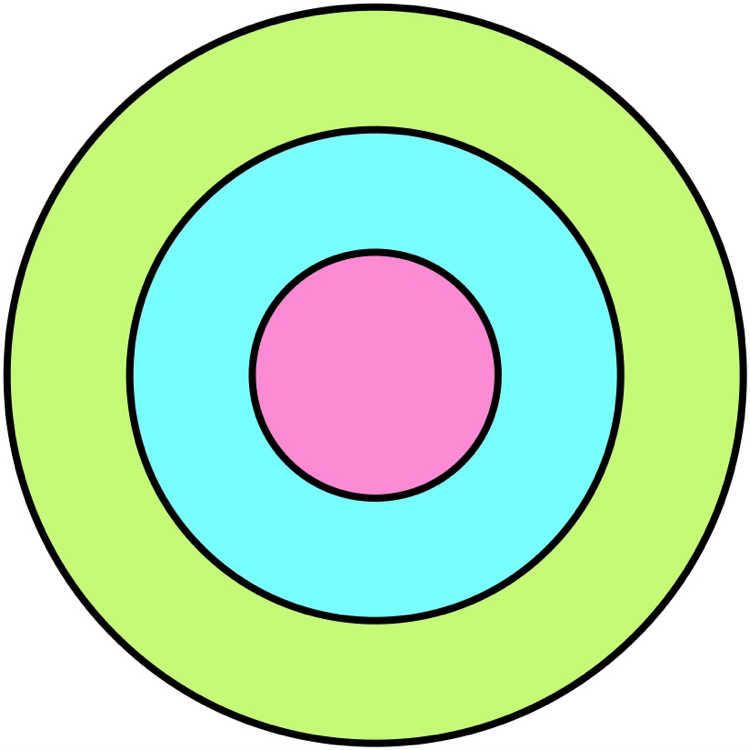
\includegraphics[width=0.75\linewidth]{chapters/chapter 8/concentric circles.png}
\caption*{$r$ շառավղով շրջանի մակերեսն է $\pi r^2$}
\end{marginfigure}

Դե իսկ եթե պատկերները ոչ թե հատվածներ են, այլ երկչափ պատ\-կեր\-ներ, երկարության փոխարեն կբաժանենք դրանց \href{http://qarakusi.am/lesson/119}{մակերեսները}։

\question{Շրջանների շառավիղներն են $1$, $2$ և $3$։ Որքա՞ն է հավա\-նա\-կան, որ պատահականորեն ընտրված կետը կգտնվի վարդագույն շրջանի մեջ։}

Երկրաչափորեն լուծենք մի փոքր ավելի հետաքրքիր խնդիր, որն առաջին հայացքից այնքան էլ երկրաչափական տեսք չունի։ 

Ենթադրենք հայտնի է, որ ավտոբուսը կանգառ է ժամանում $12$:$00$-$13$:$00$ ժամանակահատվածում ինչ-որ պատահական պահի, $5$ րոպե սպասում և շարժվում։ Մենք նույնպես կանգառ ենք գալիս $12$:$00$-$13$:$00$ ընկած որևէ պատահական պահի, սպասում մինչև $20$ րոպե, և եթե $20$ րոպեից ավտոբուսը չի գալիս, ոտքով հեռանում։ Փորձենք պարզել, թե որքա՞ն է հավանականությունը, որ ավտոբուս կնստենք։

Նախ որո՞նք են հնարավոր ելքերը։ Քանի որ ունենք երկու անհայտ մեծություններ, որոնք պատահական արժեքներ են ընդունում $12$:$00$-ից $13$:$00$-ի միջև, կամ որ նույնն է՝ $[0, 60]$ միջակայքում, ապա բոլոր ելքերը կարող ենք պատկերել $60 \times 60$ քառակուսու միջոցով՝
\begin{figure}[h]
\centering    
\caption*{սա մեր $\Omega$-ն է}
\begin{tikzpicture}[scale=0.05]  
  \draw[thick] (0,0) rectangle (60,60);
  
  \node[left] at (0,60) {$60$};
  \node[below] at (60,0) {$60$};
  \node[below] at (30,0) {$x$};
  \node[left] at (0,30) {$y$};
  \node[below left] at (0,0) {$0$};
\end{tikzpicture}    
\end{figure}

Հարմարության համար $x$-ով նշանակենք մեր գալու պահը, իսկ $y$-ով՝ ավտոբուսինը․ $(6, 34)$ կետը, օրինակ, ցույց կտա այն ելքը, երբ մենք կանգառ ենք հասել $12$:$06$ րոպեին, իսկ ավտոբուսը $12$:$34$-ին։ Իհարկե այդ իրավիճակում մենք դեռևս $12$:$26$ գնացած կլինենք և ավտոբուս չենք նստի։

Ո՞ր պատկերը ցույց կտա ավտոբուս նստելու պատահույթը։ Որպեսզի ավտոբուս նստենք, հարկավոր է, որ նախ մենք չուշանանք, այսինքն՝ գանք ավտոբուսի գնալուց ոչ ավել, քան $5$ րոպե հետո․
\[
y - x = \Big(\;\text{մեր գալու պահը}\;\Big) - \Big(\;\text{ավտոբուսի գալու պահը}\;\Big) \le 5
\]
կամ որ նույնն է՝ $y \le x + 5$։ Ուրեմն ավտոբուս նստելու համար $y$-ը պետք է գտնվի $y=x+5$ ուղղից ներքև։

\begin{figure}[t]
\centering

\begin{minipage}{0.48\textwidth}
\centering
\begin{tikzpicture}[scale=0.05]
  \fill[myLavender]
    (0,0) -- (0,5) -- (55,60) -- (60,60) -- (60,0) -- cycle;
  \draw[thick] (0,5) -- (55,60); 
  \draw[thick] (0,0) rectangle (60,60);
  \node[left] at (0,60) {$60$};
  \node[below] at (60,0) {$60$};
  \node[below] at (30,0) {$x$};
  \node[left] at (0,30) {$y$};
  \node[below left] at (0,0) {$0$};
  \node[rotate=45] at (27,40) {\small $y = x + 5$};
\end{tikzpicture}
\end{minipage}
\hfill
\begin{minipage}{0.48\textwidth}
\centering
\begin{tikzpicture}[scale=0.05]
  \fill[myOrange]
    (0,0) -- (0,60) -- (60,60) -- (60,40) -- (20,0) -- cycle;
  \draw[thick] (20,0) -- (60,40);
  \draw[thick] (0,0) rectangle (60,60);
  \node[left] at (0,60) {$60$};
  \node[below] at (60,0) {$60$};
  \node[below] at (30,0) {$x$};
  \node[left] at (0,30) {$y$};
  \node[below left] at (0,0) {$0$};
  \node[rotate=45] at (43,15) {\small $y = x - 20$};
\end{tikzpicture}
\end{minipage}

\end{figure}

Մյուս կողմից՝ եթե գանք ավտոբուսից $20$+ րոպե շուտ, ապա $20$ րոպեից կշարունակենք քայլել և նորից չենք նստի ավտոբուս։ Ուրեմն ավտոբուս նստելու համար հարկավոր է, որ
\[
x - y = \Big(\;\text{ավտոբուսի գալու պահը}\;\Big) - \Big(\;\text{մեր գալու պահը}\;\Big) \le 20
\]
կամ որ նույնն է՝ $y \ge x - 20$․ $y$-ը գտնվի $y=x-20$ ուղղից վերև։

Երկրաչափորեն այս տիրույթներից յուրաքանչյուրը մեր քառակուսու մեջ ընկած ինչ-որ հնգանկյուններ են, և այն կետերը, որոնք միաժամանակ երկուսում էլ գտնվում են, հենց այն ելքերն են, երբ ոչ մենք ենք ուշանում, ոչ ավտոբուսը։ Հետևաբար մեզ անհրաժեշտ ելքերի բազմությունը այս հնգանկյունների հատումն է՝

\begin{figure}[h]
\centering
\begin{tikzpicture}[scale=0.05]  
  \fill[mygreen, opacity=0.7]
    (0,0)     
    -- (0,5)  
    -- (55,60)
    -- (60,60)
    -- (60,40)
    -- (20,0) 
    -- cycle;
  \draw[thick] (0,5) -- (55,60); 
  \draw[thick] (20,0) -- (60,40);
  \draw[thick] (0,0) rectangle (60,60);
  \node[left] at (0,60) {$60$};
  \node[left] at (0,7.5) {$5$};
  \node[below] at (60,0) {$60$};
  % \node[below] at (30,0) {$x$};
  \node[below] at (20,0) {$20$};
  % \node[left] at (0,30) {$y$};
  \node[below left] at (0,0) {$0$};
\end{tikzpicture}
\caption*{սպիտակ եռանկյունների էջերը՝ $55$ և $40$}
\end{figure}

որի մակերեսը բաժանելով ամբողջ քառակուսու մակերեսին՝ կստանանք ավտոբուս նստելու հավանակա\-նու\-թյունը․
\[
\PP[\text{ավտոբուս նստել}] 
= 
\frac{\text{\color{mygreen} կանաչ մաս}}{\text{ընդհանուր}}
=
\frac{60^2-\frac{55^2}{2}-\frac{40^2}{2}}{60^2}
=
\frac{103}{288} \approx 0.36
\]


\bigskip 

\begin{theory}
.
\begin{itemize}
\item կարդալ [{\rm Grimmett-Welsh}], 3-5 էջերը (պատահույթներ)
\item կարդալ [{\rm Blitzstein-Hwang}], 8-13 (օրինակներ), 20-23 (հա\-վա\-նա\-կա\-նություն) էջերը 
\item ըստ ցանկության՝ [{\rm Grimmett-Welsh}], 6-10 էջերը
\item վերադառնալ [{\rm Blitzstein-Hwang}], 42-43, 49-52, 56-57 կամ [{\rm Grimmett-Welsh}], 11-15 էջերին
\item տեսնել հավանականության հաշվման տարբեր \href{https://dlsun.github.io/skis/foundations/classical-probability.html}{օրինակներ}
\item խաղալ \href{https://setosa.io/conditional}{պայմանական հավանականության} հետ 
\item դիտել {\rm 3b1b}-ի \href{https://www.youtu.be/HZGCoVF3YvM
}{տեսադասը} Բայեսի բանաձևի մասին
\item ըստ ցանկության՝ նաև մեկ այլ \href{https://youtu.be/R13BD8qKeTg}{տեսանյութ} 
\end{itemize}
\end{theory}

\newpage

\section{Խնդիրներ}

\begin{problem}
Նետում ենք երկու զառ։ Որքա՞ն է հավանականությունը, որ կընկնի
\begin{enumerate}[label={\alph*}․]
\item երկուսն էլ $3$
\item գոնե մեկ հատ $1$
\item ուղիղ մեկ հատ $1$
\item մեկ հատ $1$, մեկ հատ $4$
\item առաջինը՝ $1$, երկրորդը՝ $4$
\end{enumerate}
\end{problem}

\begin{problem}
Գրչատուփի մեջ կա $2$ սև, $5$ կապույտ և $6$ դեղին մատիտ։ Պատահականորեն վերցնում ենք դրանցից երկուսը։ Որքա՞ն է հավանա\-կան, որ երկու մատիտն էլ 
\begin{enumerate}[label={\alph*}․]
\item կարմիր կլինեն
\item նույն գույնի կլինեն
\item տարբեր գույների կլինեն
\item դեղին չեն լինի
\item կանաչ չեն լինի
\end{enumerate}
\end{problem}

\begin{problem}
\begin{marginfigure}
    \centering
    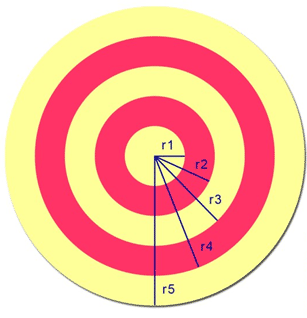
\includegraphics[width=\linewidth]{chapters/chapter 8/darts.png}
\end{marginfigure}
Նկարում պատկերված թիրախը կազմված է համապատաս\-խանաբար $1$, $2$, $3$, $4$ և $5$ սմ երկարությամբ շրջաններից։ Պատա\-հականորեն հարվածում ենք թիրախին։ Որքա՞ն է հավանականությունը, որ կդիպչենք
\begin{enumerate}[label={\alph*}․]
\item ամենափոքր շրջանին
\item կարմիր շրջանի
\item դեղին շրջանի
\end{enumerate}
\end{problem}

\begin{problem}
Մետաղադրամը նետում ենք $5$ անգամ։ Որքա՞ն է հավանակա\-նությունը, որ կենտ անգամ կընկնի գիր։
\end{problem}

\begin{problem}
Գրապահարանում կա $15$ գիրք, որոնցից $5$-ը հայերեն են, $10$-ը՝ ֆրանսերեն։ Ռուբենը ֆրանսերեն չգիտի։ Նա պատահականորեն վերցնում է $3$ գիրք։ Որքա՞ն է հավանականությունը, որ նա դրանցից գոնե մեկը կարող է կարդալ։
\end{problem}

\begin{problem}
Երեք անգամ նետում ենք զառը։ $A$, $B$, $C$-ով նշանակենք հետևյալ պատահույթները՝
\begin{itemize}
    \item $A$ $=$ գոնե մեկ անգամ ընկել է զույգ թիվ
    \item $B$ $=$ գոնե մեկ անգամ ընկել է $3$-ի պատիկ թիվ
    \item $C$ $=$ գոնե մեկ անգամ ընկել է $5$
\end{itemize}
Որքա՞ն է հավանականությունը, որ այս երեքից գոնե մեկը տեղի կունենա։
\end{problem}

\begin{problem}
Առաջին տուփում կա համապատասխանաբար $\{5, 11, 8\}$ սև, դեղին, կարմիր մատիտ, իսկ երկրորդում՝ $\{10, 8, 6\}$։ Յուրաքանչյուր տուփից պատահականորեն վերցնում ենք մեկական մատիտ։ Որքա՞ն է հավանականությունը, որ երկուսն էլ կլինեն նույն գույնի։
\end{problem}

\begin{problem}
Նետում ենք երկու զառ։ Որքա՞ն է հավանական, որ դրանցից մեկը կընկնի $1$, եթե գիտենք, որ դրանց գումարը զույգ է։
\end{problem}

\begin{problem}
$52$ խաղաթղթերից\marginnote[*+1.8]{հայերեն՝ քյափ}  պատահական վերցնում ենք $3$-ը։ Որքա՞ն է հավանականությունը, որ առաջին երկուսը կլինեն թագուհի (դամա), իսկ երրորդը՝ {\color{myred}$\blacklozenge$} աղյուս։
\end{problem}

\begin{problem}
Ցանկանում ենք գրել սպամերը հայտնաբերող ծրագիր։
Հայտնի է, որ
\begin{itemize}
    \item սպամ նամակների $80\%$-ը պարունակում է «շահեք» բառը
    \item ոչ սպամ նամակների $30\%$-ն է պարունակում «շահեք» բառը
    \item միջինում նամակների $40\%$-ը սպամ է
\end{itemize}
Ճիշտ այդ պահին ստանում ենք նամակ, որը պարունակում է «շահեք» բառը։ Որքա՞ն է հավանական, որ այն սպամ է։
\end{problem}

\begin{problem}
Երեք նորածինների տանում են ստուգելու, այնուհետև պատահականորեն վերադարձնում իրենց մայրերին։ Որքա՞ն է հավանա\-կանությունը, որ փոքրիկներից գոնե մեկին կվերադարձնեն իր մայրիկին։
\end{problem}

% \begin{problem}
% Suppose that you know the answers to 20 questions out of the total 25
% questions in the entrance examination, from which you are only asked
% 3 random questions. What is the probability that you answer all of
% the questions?

% \begin{problem}
% There are two boxes containing {5, 11} and {10, 8} white, black balls
% respectively. First, we take out a ball from each of the boxes. Then, we randomly choose one of them. What is the probability that the
% final ball is white?

% \begin{problem}
% There are three boxes having 4 white and 6 black balls in each of them.
% Suppose we perform the following steps in the given order:
%     \begin{enumerate}
%         \item[a) ] take out a ball from the first box and put it into the second one,
%         \item[b) ] take out a ball from the second box and put it into the third one,
%         \item[c) ] take out a ball from the third box and put it into the first one.
%     \end{enumerate}
%     What is the probability of taking a white ball from the third box (after doing \textit{a)-c)})?

\begin{problem}
Առաջին գործարանը երկրորդից $2$ անգամ ավելի շատ զենքեր է արտադրում։ Հայտնի է, որ 
\begin{itemize}
    \item առաջինում արտադրված զենքերի $40\%$-ը խոտան է
    \item երկրորդում արտադրվածների $16\%$-ն է խոտան
\end{itemize}
Պատահականորեն ստուգում ենք զենքերից մեկն ու պարզում, որ այն խոտանված չէ։ Որքա՞ն է հավանականությունը, որ այն արտադրել են առաջին գործարանում։
\end{problem}

\begin{problem}
Արձակուրդի գնալիս հարևանին խնդրում եք ամեն օր ջրել Ձեր ծաղիկները։ Եթե ծաղիկներն ամեն օր ջրեն, ապա $0.85$ հա\-վա\-նականությամբ դրանք կշարունակեն ծաղկել, մինչդեռ եթե չջրեն, ապա գոյատևելու հավանականությունն ընդամենը $0.2$ է։ Գրեթե $90\%$-ով համոզված եք, որ Ձեր հարևանը կջրի ծաղիկները, սակայն արձակուրդից վերադառնալով՝ տեսնում եք, որ ծաղիկները թառամել են։ 

Որքա՞ն է հավանական, որ հարևանը մոռացել է ջրել ծաղիկները։ Կշարունակե՞ք վստահել նրան։
\end{problem}

\begin{problem}
Նունեն դեպքերի $30\%$ տոկոսում մեքենայով է գործի գալիս, $30\%$-ում՝ ոտքով, իսկ մնացած $40\%$-ում գալիս է ավտոբուսով։ Ընդ որում,
\begin{itemize}
    \item ոտքով գալիս ուշանում է դեպքերի $10\%$-ում
    \item մեքենայով գալիս՝ $3\%$-ում
    \item ավտոբուսով գալիս՝ $7\%$-ում
\end{itemize}
Երեկ Նունեն ուշացել է։ Որքա՞ն է հավանականությունը, որ նա ավտո\-բու\-սով էր գալիս։ Որքա՞ն է հավանական, որ այսօր նա ոտքով էր, եթե այսօր ճիշտ ժամանակին է եկել։
\end{problem}

\begin{problem}
Անգետիկն ունի $10$ մետաղադրամ, որոնցից $9$-ը սովորական են, իսկ $1$-ի երկու կողմն էլ գիր է։ Նա պատահականորեն վերցնում է մետաղադրամներից մեկը․
\begin{enumerate}[label={\alph*}․]
\item որքա՞ն է հավանականությունը, որ դա կեղծ մետաղադրամն է

\item եթե նա նետի մետաղադրամն, ու այն գիր ընկնի, որքա՞ն է հավանականությունը, որ դա կեղծն է

\item եթե նա նետի մետաղադրամն, ու այն ղուշ ընկնի, որքա՞ն է հավանականությունը, որ դա $9$ սովորականներից մեկն է
\end{enumerate}
\end{problem}

\begin{problem}
Գառնի-Գեղարդից վերադառնալով՝ Ձեր տեսախցիկը տանում եք արհեստանոց՝ լուսանկարները մշակելու։ Ցավոք, արհես\-տա\-նոցում ժապավենը փչացնում են, և ընդհանուր $24$ կադրերից $4$ հաջոր\-դական կադրեր վնասվում են։ Որքա՞ն է հավանականությունը, որ վնասված կադրերի թվում են
\begin{enumerate}[label={\alph*}․]
\item ութերորդ, իններորդ կամ տասներորդ լուսանկարները
\item ութերորդ, իններորդ և տասներորդ լուսանկարները
\end{enumerate}
\end{problem}

\begin{problem}\marginnote[*+0.5]{\href{https://youtu.be/U2AE4TZU4MA}{լուծում}}
Անուշն ու Նաիրին ժամը $12$:$00$-ից $13$:$00$ որևէ պատահական պահի գալիս են «Մոսկվա» կինոթատրոնի մոտ և սպասում մյուսին՝ միասին ընդմիջման գնալու համար։ Եթե երկրորդը $15$ րոպեից ավել է ուշանում, առաջինը տեղ հասնողը միայնակ է գնում ընդմիջման։ 

Որքա՞ն է հավանականությունը, որ նրանք միասին կընդմիջեն, եթե երկուսի համար էլ $12$:$00$-$13$:$00$ բոլոր պահերը հավասարահավանական են։
\end{problem}


\setchapterpreamble[u]{\margintoc}
\chapter{Պատահական մեծություններ}
\labch{random_variables}

\emergencystretch 2em

\section{Ֆորմալ սահմանումը}

Նախորդ թեմայի վերջին խնդիրը լուծելիս ունեինք երկու անհայտ մեծություններ՝ ավտոբուսի գալու ժամանակն ու մեր գալու ժամանակը, որոնց արժեքը հայտնի չէր (ընդունում էին պատահական արժեքներ), սակայն գիտեինք, թե որոնք էին դրանց հավանական արժեքները, այնպես որ դրանք նշանակեցինք տառերով ու լուծեցինք խնդիրը։ Նմանատիպ մեծությունները, որոնց արժեքը չգիտենք, բայց կարող ենք \textit{հաշվել,} թե ինչ հավանականությամբ են ընդունում այս կամ այն արժեքը, \marginnote{անգլերեն՝ {\it random variables}} կոչվում են \textit{պատահական մեծություններ։}

\question{Փողոցում մոտենում եք պատահական անցորդի ու հարց\-նում նրա հասակը։ Մոտավորապես ո՞ր միջակայքի արժեքներն են ավելի շատ հավանական, որո՞նք՝ ավելի քիչ։}

Եթե փորձենք ավելի ճշգրիտ ձևակերպում տալ, կարող ենք փողոցում քայլող բոլոր հնարավոր մարդկանց բազմությունը համարել մեր $\Omega$-ն, և ասել, որ պատահական ընտրված ցանկացած մարդու համապատասխա\-նեց\-րել ենք ինչ-որ մի թիվ՝ նրա հասակը։ Կամ որ նույնն է՝ ստեղծել ենք $X$ ֆունկցիա, որը վերցնում է $\omega$ մարդուն ու վերադարձնում նրա հասակը՝ $X(\omega)$։ 

\begin{example}\label{die_game}
Խաղում ենք հետևյալ խաղը․ նետում ենք զառը, պարզ թիվ ընկնելու դեպքում շահում ենք $100$ դրամ, բաղադրյալ թվի դեպքում՝ կորցնում $100$, հակառակ դեպքում՝ լինում է ոչ-ոքի։ Այս դեպքում մեր վերջնական շահումը/կորուստը կլինի պատահական մեծություն։ 

Եթե նշանակենք այն $X$-ով, ապա $X$-ը կընդունի երեք արժեք՝
\[ X  =
\begin{cases}
100 & \text{եթե } \omega \in \{2, 3, 5\} \\
-100 & \text{եթե } \omega \in \{4, 6\} \\
0 & \text{եթե } \omega \in \{1\}
\end{cases}
\]
Կարո՞ղ եք հաշվել հավանականությունը, որ $X=100$։
\end{example}

Առհասարակ՝ ցանկացած բան, որի արժեքը կախված է ինչ-որ  պատահական փորձի արդյունքից, հանդիսանում է պատահական մեծություն։

\begin{example}\label{rv_examples}
Դիտարկենք հետևյալ պատահական փորձերը․

\begin{enumerate}
\item Նետում ենք երկու զառ։ Դրանց ելքերի գումարը պատահական մեծություն է։

\item Երկու թիմ խաղում են ֆուտբոլ։ Նրանց խփած գոլերի թիվը, ինչպես նաև հաշվի տարբերությունը պատահական մեծու\-թյուններ են։ 

\item Զանգահարում ենք պատահական հեռախոսահամարով և հարցնում, թե քանի երեխա կա ընտանիքում․ սա նույնպես պատա\-հական մեծություն է։

\item Ընդհանուր քանի հաղորդագրություն կստանաք վաղը՝ պատա\-հական մեծություն է։

\item Երկու ավտոբուս պատահական պահերի անցնում են կանգառով։ Դրանցից յուրաքանչյուրի գալու պահը, ինչպես նաև այդ երկու պահերի տարբերությունը պատահական մեծություններ են։

\item Որքան կլինեն «{\rm Apple}»-ի արժեթղթերը հաջորդ շաբաթ՝ պատահական մեծություն է։

\item $xy$-հարթության վրա պատահական նշված կետի երկու կոոր\-դի\-նատները, նաև այդ կետի հեռավորությունը, ասենք, $(5, 3)$ կետից՝ պատահական մեծություններ են։
\end{enumerate}
\end{example}

\question{Որո՞նք են նշված պատահական մեծություններից յուրա\-քան\-չյուրի հնարավոր արժեքները։}

\begin{example}
Նետում ենք երկու զառ։ Այն, թե
\begin{itemize}
    \item ո՞վ է նետել զառերը
    \item ի՞նչ գույն ունի երկինքը
    \item ինչո՞ւ է աղմկում գետը
    \item ի՞նչ թիվ է ընկել երրորդ զառը
\end{itemize}
պատահական մեծություններ \textit{չեն,} քանի որ դրանք \textit{կախված չեն} կատարված փորձի արդյունքից․ եթե նույնիսկ իմանայինք, թե ինչ են ընկել զառերը, այս հարցերին չէինք կարող պատասխանել։
\end{example}

Այսպիսով, ինտուիտիվ դժվար չէ հասկանալ, թե այս կամ այն խնդրում ինչն է պատահական մեծություն։ \marginnote{այսինքն՝ չափել, թե որքան է հավանա\-կան, որ $X$-ի արժեքը կլինի այս կամ այն բազմությունից (թե չէ ամբողջ տեսու\-թյունն անիմաստ կդառնար)}
Եթե այնուամենայնիվ փորձենք ավելի ճշգրիտ սահմանել, կասենք, որ ցանկացած այնպիսի $X$, որի արժեքների հավանականությունը կարող ենք չափել, պատահական մեծություն է։

\warning{Առջևում սպասվում է տեսական բնույթի քննարկում։}

Իսկ հավանականությունը չափելու համար անհրաժեշտ է մեկ բան։ Որպեսզի, օրինակ, կարողանանք հաշվել, թե ինչ հավանականությամբ է $X$-ը ընդունում $1.57$ արժեքը՝ 
\[
\PP[X = 1.57]
\]
անհրաժեշտ է, որ $\PP[\quad]$-ի մեջ գրվածը լինի պատահույթ, այսինքն՝
\[
\{X = 1.57\} = \{ \text{այն $\omega$-ները, որոնց համար }X = 1.57 \} \in \F
\]
Նույն ձև բնականաբար պետք է կարողանանք չափել $\PP[X < 1.57]$, $\PP[X > 1.57]$, $\PP[X \le 1.57]$ և մնացած այլ հավանականությունները։

\question{Ունենալով $\PP[X \le 1.57]$-ը՝ կարո՞ղ եք հաշվել $\PP[X > 1.57]$-ը։}

Ուրեմն ֆորմալ կպահանջենք, որ ասենք՝ $\{X \le 1.57\}$ բազմությունը լինի պատահույթ ($=$ հնարավոր լինի չափել դրա հավանականությունը), կամ ընդհանուր դեպքում՝ ցանկացած $c$ թվի համար
\[
\{X \le c\} = \{ \text{այն $\omega$-ները, որոնց համար }X \le c \} \in \F
\]
լինի պատահույթ։ \marginnote{կարող ենք իհարկե $\le$-ի փոխարեն գրել $<$, $>$ կամ $\ge$} Ահա այս պայմանին բավարարող ցանկացած $X$ կանվանենք պատահական մեծություն։

Նշենք, որ հետագա կիրառություններում բավարար է ընդամենը համա\-րել, որ ցանկացած անհայտ, բայց խելքին մոտիկ բան պատահական մեծություն է։ 

Նկատենք նաև, որ եթե $X$-ը ինչ-որ մի պատահական մեծություն է, ապա նրա հետ գործողություններ անելիս՝
\begin{itemize}
    \item $2X$-ը
    \item $X+4$-ը
    \item $X^2$-ն
    \item $e^X$-ը
\end{itemize}
և այլն նույնպես կլինեն պատահական մեծություններ։ 

Ավելի ընդհանուր,
\begin{theorem}\label{transformed_rv}
Եթե $X$-ը պատահական մեծություն է, ապա $g(X)$-ը նույնպես պատահական մեծություն է (ցանկացած $g$ անընդհատ ֆունկցիայի համար)։
\end{theorem}



\section{Դիսկրետ պատահական մեծություններ}

Ինչպես նկատում ենք, որոշ պատահական մեծությունների հնարավոր ար\-ժեքները կարելի է ներկայացնել ցուցակի տեսքով, օրինակ՝ $\{2, 3, 4, \linebreak \dots, 12\}$ կամ $\{0, 1, 2, \dots\}$, իսկ որոշներինը՝ միջակայքերի՝ $(0, +\infty)$։

Եթե պատահական մեծության հնարավոր արժեքների բազմությունը
\begin{itemize}
    \item վերջավոր է՝ $\{x_1, x_2, \dots, x_n\}$, կամ անվերջ, բայց հաշվելի՝ $\{x_1, x_2, \dots, x_n, \dots\}$, \marginnote{այսինքն անվերջ, բայց միջակայքեր չպարունակող, օրինակ՝ $\N$-ը}ապա այն կանվանենք \textit{դիսկրետ} կամ \textit{ընդհատ}

    \item իսկ եթե այն ինչ-որ միջակայք է՝ $(a,b)$ կամ $[a, b]$ (կամ դրանց միավորում), ապա այն կանվանենք \textit{անընդհատ}
\end{itemize} 

Մասնավորապես, ցանկացած բանի քանակ ցույց տվող պատահական մեծությունները դիսկրետ են, իսկ ժամանակ կամ երկարություն ցույց տվողները՝ անընդհատ։ \hyperref[rv_examples]{{\color{OliveGreen} Օրինակ \ref*{rv_examples}}}-ի 1-4 դեպքերում պատահական մեծությունները դիսկրետ են, 5-7-ում՝ անընդհատ։

\question{$X$-ով նշանակենք զառի թվի մնացորդը $3$-ի բաժանելիս․
\begin{itemize}
    \item ի՞նչ հնարավոր արժեքներ կարող է այն ընդունել
    \item որքա՞ն է դրանցից յուրաքանչյուրի հավանականությունը
    \item որքա՞ն է հավանական, որ $X=5$
\end{itemize}}

Իհարկե, եթե որևէ անհայտ բան նշանակել ենք $X$-ով, նախ և առաջ կուզեինք պարզել, թե որքան է հավանական, որ այն կընդունի այսինչ արժեքը։ Վերցնենք ասենք՝ \hyperref[die_game]{{\color{OliveGreen} օրինակ \ref*{die_game}}}-ի խաղում մեր շահույթը ցույց տվող $X$ պատահական մեծությունը․
\[ 
X  =
\begin{cases}
100 & \text{եթե } \omega \in \{2, 3, 5\} \\
-100 & \text{եթե } \omega \in \{4, 6\} \\
0 & \text{եթե } \omega \in \{1\}
\end{cases}
\]

Որքա՞ն է հավանականությունը, որ կշահենք $100$ դրամ, այսինքն՝
\[
\PP[X = 100] =\  ? 
\]
Քանի որ $X$-ը $100$ արժեքը ընդունում է $\{2, 3, 5\}$ ելքերի դեպքում, $X=1$-ի հավանականությունը կլինի հենց այդ պատահույթի հավանականու\-թյու\-նը՝
\[
\PP[X = 100] = \PP[\{2, 3, 5\}] = \frac{3}{6} = 0.5
\]
իսկ օրինակ ոչ-ոքիի հավանականությունը՝
\[
\PP[X = 0] = \PP[\{1\}] = \PP[1] = \frac{1}{6}
\]
Հետևյալ արտահայտությունը՝
\[
\PP[X = \text{ինչ-որ թիվ}]
\]
որը վերևում հաշվեցինք, ըստ էության ֆունկցիա է, որը վերցնում է $c$ թիվն ու վերադարձնում $X$-ի՝ այդ $c$ թվին հավասար լինելու հավանականությունը՝
\[
p_X(c) = \PP[X = c]
\]
այսինքն հաշվում, թե որքան է հավանական, որ ${X=c}$։ Այդ $p_X$ ֆունկ\-ցիան կանվանենք $X$-ի \textbf{հավանականային ֆունկցիա} կամ {\bf PMF:}\marginnote{{\it probability mass function}}

\question{Ենթադրենք $X$-ը հենց զառը նետելիս ստացվող թիվն է։ Կարո՞ղ եք գրել կամ պատկերել դրա հավանականային ֆունկցիան։}

{\rm PMF}-ի շնորհիվ, օրինակ՝ եթե ունենք դրա գրաֆիկը, կարող ենք պատ\-կե\-րացում կազմել, թե ի՞նչ արժեք\-ներ է ընդունում $X$-ը, արժեքներից ո՞րը ի՞նչ հավանականությամբ, և այլն։

\question{Քանի՞ ֆիլմ եք դիտելու հաջորդ ամիս։ Պատասխանը նշա\-նա\-կենք $X$-ով և գծենք նրա {\it PMF}-ի գրաֆիկը։ Որքա՞ն է հավա\-նական, որ կդիտեք $5$-$6$ ֆիլմ։ Քանի՞ ֆիլմն է ամենահավանականը։}

\begin{figure}[b]
    \centering
    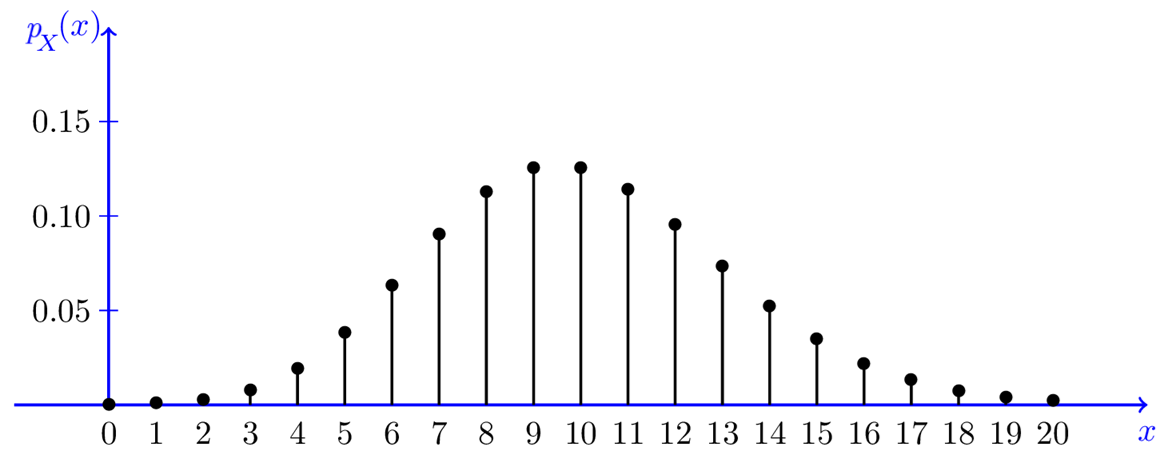
\includegraphics[width=0.8\linewidth]{chapters/chapter 9/PMF graph.png}
\end{figure}

\begin{example}
Ուսանողը գիտի հարցաշարի $15$ թեմաներից $4$-ը, ընդ որում քննության ժամանակ տրվելու է $2$ հարց։ $X$-ով նշանակենք, թե այդ երկու հարցից քանիսին կպատասխանի ուսանողը, և հաշվենք $X$-ի {\rm PMF}-ը։

Հավանականությունը, որ ուսանողը ոչ մի հարցի չի պատասխանի, նույնն է, ինչ եթե և՛ առաջին, և՛ երկրորդ հարցերը լինեն նրա չիմացած հարցերից․\marginnote[*+1]{$\Rightarrow$ պետք էր ժամանակին սովորել}
\[
\PP[X=0] = \frac{11}{15} \cdot \frac{10}{14} = \frac{11}{21} \approx 0.52
\]
իսկ որպեսզի երկուսին էլ կպատասխանի, անհրաժեշտ է, որ և՛ առաջինը, և՛ երկրորդը լինեն իր իմացածներից․
\[
\PP[X=2] = \frac{4}{15} \cdot \frac{3}{14} = \frac{6}{105} \approx 0.06
\]
Մնաց մի դեպք՝ երկու հարցից ուղիղ մեկին պատասխանելու դեպքը, որի հավանականությունը կլինի\marginnote{կարող էինք հաշվել նաև այսպես՝ \[\PP[X=1] = \frac{4}{15} \cdot \frac{11}{14} + \frac{11}{15} \cdot \frac{4}{14}\]}
\[
\PP[X=1] = 1 - \PP[X=0] - \PP[X=2] 
% = 1 - \frac{11}{21} - \frac{6}{105} 
= \frac{44}{105} \approx 0.42
\]\begin{marginfigure}[*+4]
    \centering
    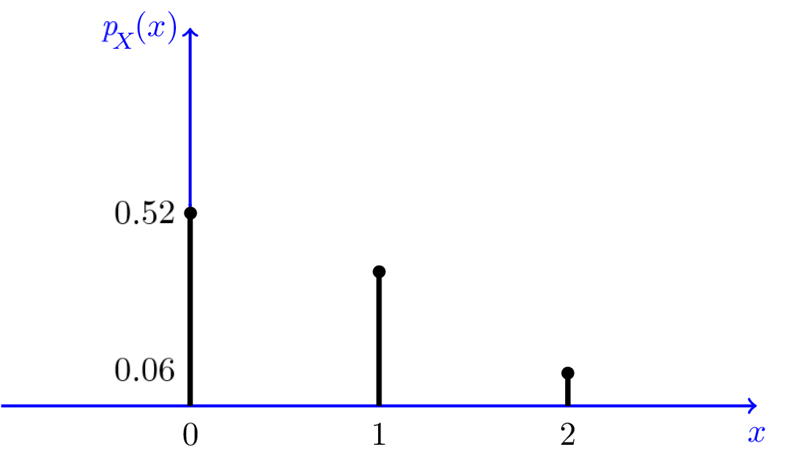
\includegraphics[width=\linewidth]{chapters/chapter 9/PMF graph exam.png}
\end{marginfigure}
Հետևաբար $X$-ի {\rm PMF}-ն է՝
\[
p_X(k) \approx \begin{cases}
    0.52 & \text{եթե } k = 0\\
    0.42 & \text{եթե } k = 1\\
    0.06 & \text{եթե } k = 2\\
    0 & \text{եթե $k$-ն այլ թիվ է}
\end{cases}
\]
որը ցանկության դեպքում կարող ենք ներկայացնել աղյուսակով՝
\begin{center}
% \begin{table}[h]
  % \centering
  % \raggedright
  \begin{tabular}{|c|c|}
    \hline
    $k$ & $\PP[X=k]$ \\
    \hline
    $0$ & $0.52$ \\
    \hline
    $1$ & $0.42$ \\
    \hline
    $2$ & $0.06$ \\
    \hline
  \end{tabular}
% \end{table}
\end{center}
\end{example}


\section{Բաշխման ֆունկցիա}

Հավանականային ֆունկցիան, իհարկե, կարևոր է իմանալ, բայց այս իրավիճակում ուսանողին հետաքրքրում է ոչ այնքան իր պատասխանած հարցերի թիվը, որքան քննության արդյունքը՝ կկտրվի՞, թե՞ ոչ։ 

Եթե օրինակ՝ անցողիկ շեմը լիներ ճիշտ պատասխանել $1$ հարցի, կտրվելու հավանականությունը կլիներ
\[
\PP[X < 1] = \PP[X = 0] \approx 0.52
\]
իսկ եթե լիներ $2$ հարց՝
\[
\PP[X < 2] = \PP[X = 0] + \PP[X = 1] \approx 0.94
\]
Գոյատևելու շանսերը կլինեին համապատասխանաբար $1-0.52=0.48$ և $1-0.94=0.06$: 

Մի ուրիշ իրավիճակում հնարավոր միավորների թիվը կարող էր լինել $1$-ից մինչև $20$՝ յուրաքանչյուր արժեքը իր հավանականությունով։ Այս դեպքում ևս, եթե ուսանողը ցանկանար հաշվել իր կտրվելու (ասենք՝ $10$ միավոր կամ ցածր հավաքելու) հավանականությունը, կգրեր
\[
\PP[X \le 10] = \PP[X = 0] + \PP[X = 1] + \dots + \PP[X = 10]
\]
իսկ քննությունը ստանալունը կլիներ $1 - \PP[X \le 10]$:

Գործնականում հաճախ է պետք գալիս առանձին-առանձին $1$, $2$, $\dots$, $k$ արժեքներն ընդունելու հավանականություններից բացի ունենալ նաև $k$-ից փոքր, մեծ, փոքր կամ հավասար լինելու հավանականությունը՝
\[
\PP[X \le k]
\]
Բայց այստեղ ևս $k$-ի տարբեր արժեքներ տեղադրելով՝ ստանում ենք տարբեր թվեր, հետևաբար գործ ունենք $k$-ից կախված ֆունկցիայի հետ։ Ուրեմն 
{\rm PMF}-ի նմանությամբ սահմանենք հետևյալ ֆունկցիան՝
\[
F_X(k) = \PP[X \le k]
\]
և անվանենք այն $X$-ի \textbf{բաշխման ֆունկցիա} կամ {\bf CDF:}\marginnote{{\it cumulative distribution function}}

\question{Ուսանողի օրինակում ինչի՞ է հավասար $X$-ի {\rm CDF}-ը։}

\begin{example}
$X$-ով նշանակենք զառը նետելիս ստացված թիվը և գտնենք դրա բաշխման ֆունկցիան։ Սկսենք $k=1$-ից՝
\[
F_X(1) = \PP[X \le 1] = \frac{1}{6}
\]
քանի որ $X$-ը $1$-ից փոքր արժեք չի կարող ընդունել։ 

Իսկ ասենք $k=2$ արժեքի դեպքում՝
\[
F_X(2) = \PP[X \le 2] = \PP[X = 1] + \PP[X = 2] = \frac{2}{6} = \frac{1}{3}
\]
Նույն կերպ $k=3$-ի համար $F_X(3) = \dfrac{3}{6}$, ապա
\[
F_X(4) = \dfrac{4}{6} \qquad F_X(5) = \dfrac{5}{6} \qquad F_X(6) = \dfrac{6}{6} = 1
\]

Իսկ ի՞նչ, եթե $F_X$-ի մեջ տեղադրենք $6$-ից մեծ թիվ, ասենք՝ $k=8$։ Կունենանք՝
\[
F_X(8) = \PP[X \le 8] = 1
\]
քանի որ $X$-ի արժեքը \textit{միշտ փոքր է} $8$-ից։ Նույն ձևով $F_X(k) = 1$ բոլոր այնպիսի $k$ թվերի համար, որոնք մեծ են $6$-ից։ 

Մյուս կողմից՝ եթե տեղադրենք $1$-ից փոքր արժեք, ասենք՝
\[
F_X(0.12) = \PP[X \le 0.12] = 0
\]
կունենանք $0$, քանի որ $X$-ը \textit{երբեք փոքր չէ} $1$-ից։ Հետևաբար $F_X(k) = 0$ բոլոր $k < 1$ թվերի համար։

Վերջապես եթե տեղադրենք ոչ ամբողջ թիվ, օրինակ՝
\[
F_X(5.5) = \PP[X \le 5.5] = \PP[\text{որքա՞ն է հավանական, որ }X \le 5.5]
\]
ապա դա կլինի նույնը, ինչ $\PP[X \le 5]$։ Հետևաբար $X$-ի {\rm CDF}-ը կլինի հետևյալ ֆունկցիան՝
\[ 
F_X(x)=
\begin{cases}
    0 &\text{եթե }x < 1\\
    1/6 &\text{եթե }1 \le x < 2\\
    2/6 &\text{եթե }2 \le x < 3\\
    3/6 &\text{եթե }3 \le x < 4\\
    4/6 &\text{եթե }4 \le x < 5\\
    5/6 &\text{եթե }5 \le x < 6\\
    1 &\text{եթե }x \ge 6
\end{cases}
\]
\end{example}

\question{Ի՞նչ տեսք ունի $F_X$-ի գրաֆիկը։}

Ինչպես երևում է, $F_X$ ֆունկցիան անընդհատ չէ։ Այն խզվում է $1$, $2$, $3$, $4$, $5$, $6$ կետերում,\marginnote{փորձեք գծել $F_X$-ի գրաֆիկը} այդ կետերի միջև ընդունում է ֆիքսված հաստատուն արժեքներ, ապա ցատկոտելով բարձրանում է ու ընդունում հաջորդ արժեքը։ 

\question{Կարո՞ղ եք $F_X$-ի գրաֆիկին նայելով որոշել նրա ընդու\-նած հնարավոր արժեքները։ Իսկ դրանցից յուրաքանչյուրի հավանա\-կա\-նու\-թյո՞ւնը։}

Նկատենք, որ 
\begin{enumerate}
    \item $F_X$-ը չնվազող ֆունկցիա է\marginnote{ո՞րն է ավելի մեծ՝
    \[\PP[X \le 10] \quad \text{թե՞} \quad \PP[X \le 10000]\]}
    \item $F_X$-ի արժեքները ընկած են $[0, 1]$ միջակայքում
    \item ընդ որում $\lim\limits_{x \to -\infty} F_X(x) = 0$ և $\lim\limits_{x \to \infty} F_X(x) = 0$
\end{enumerate}

Իրականում այս 1-3 հատկությունները ճիշտ են ոչ միայն զառի, այլ առհասարակ ցանկացած պատահական մեծության համար (և դիսկրետ, և անընդհատ)։ Ավելին, բոլոր դիսկրետ $X$-երի {\rm CDF}-ի գրաֆիկն ունի այսպիսի աստիճանաձև տեսք՝
\begin{figure}[h]
    \centering
    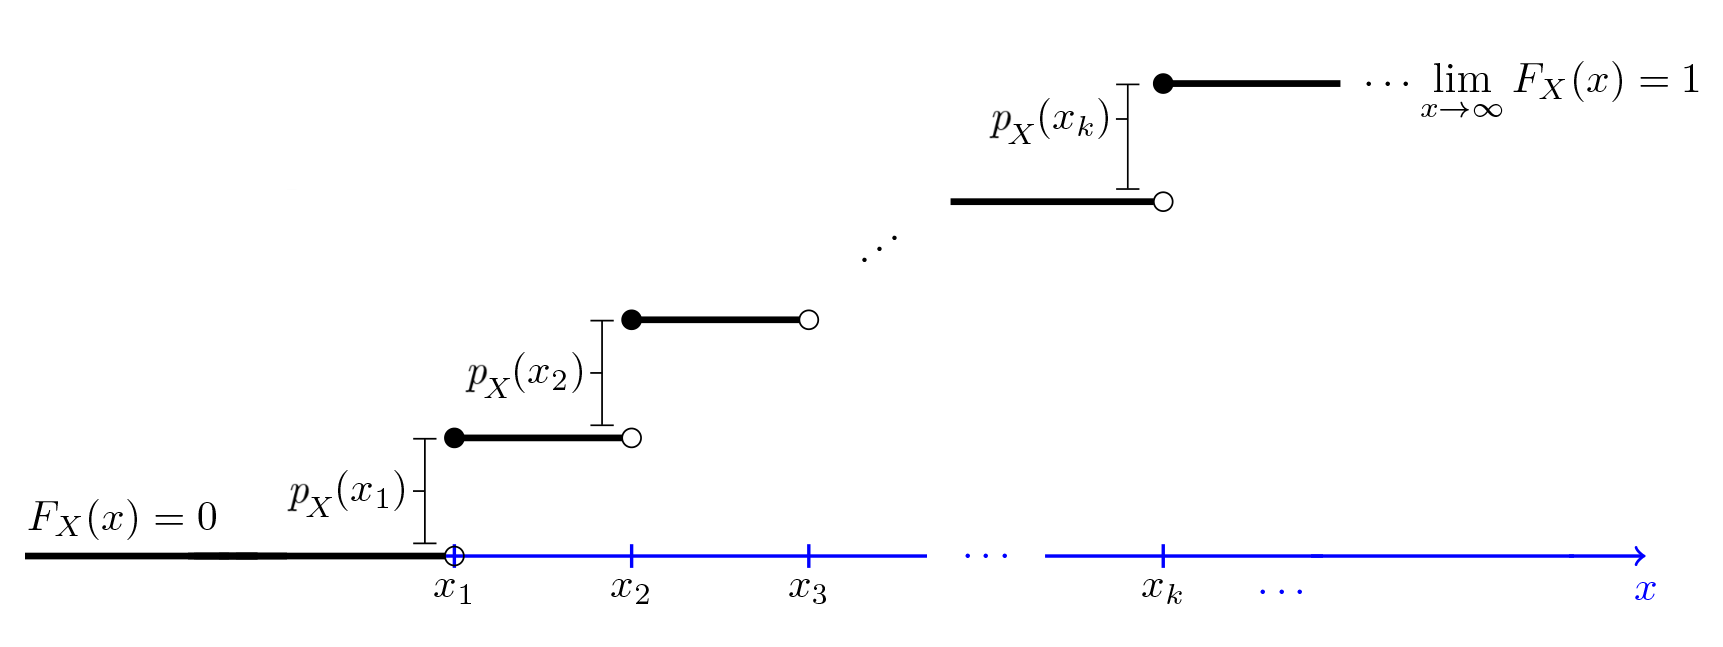
\includegraphics[width=0.8\linewidth]{chapters/chapter 9/CDF graph.png}
\end{figure}

որի խզումներին նայելիս կարելի է գլխի ընկնել, թե $X$-ը որ արժեքը ինչ հավանականությամբ \marginnote{$\PP[X=k]$-ն կգրենք $F_X(k) - F_X(k-1)$} է ընդունում։

{\rm PMF}-ը և {\rm CDF}-ը (որոնցից մեկը ունենալով՝ կարելի է ստանալ մյուսը) հարմար գործիքներ են տրված պատահական մեծության արժեքների վերաբերյալ պատկերացում կազմելու համար։ Պայմանավորվենք՝ այն, թե ի՞նչ արժեքներ է ընդունում պատահական մեծությունը, կամ որքա՞ն հավանականությամբ, կամ որքա՞ն է հավանական, որ այն մեծ/փոքր է այսինչ թվից, այդ ամենը անվանել պատահական մեծության \textit{բաշխում։}

Կասենք, որ գիտենք $X$-ի բաշխումը (կամ թե ինչպես են $X$-ի արժեքները բաշխված), եթե գիտենք նրա {\rm PMF}-ը կամ {\rm CDF}-ը։ Իսկ եթե ունենանք երկու պատահական մեծություններ, որոնք ունենան նույն բաշխումը, այսինքն՝ ցանկացած արժեք ընդունեն երկուսն էլ նույն հավանականությամբ, ապա կասենք, որ դրանք \textit{միատեսակ} են բաշխված:

\begin{definition}
$X$ և $Y$ պատահական մեծությունները կոչվում են \textbf{միատեսակ բաշխված,} \marginnote{անգլերեն՝ {\it identically distributed}} եթե նրանց {\it CDF}/{\it PMF}-ները համընկնում են։
\end{definition}

\warning{Միատեսակ բաշխված $\ne$ միմյանց հավասար։}

\begin{example}
Քննության է մտնում հաջորդ ուսանողը, որը ևս $15$ հարցից սովորել է $4$-ը։ Բնականաբար, հավանականությունը, որ նա կկտրվի կամ կանցնի քննությունը, նույնն է, ինչ առաջին ուսա\-նո\-ղի\-նը։ Հետևաբար եթե $X$-ով նշանակենք, թե քանի հարցի ճիշտ կպատասխանի առաջին ուսանողը, իսկ $Y$-ով՝ երկրորդը, ապա $p_X(k) = p_Y(k)$, և $X$-ն ու $Y$-ը կլինեն միատեսակ բաշխված։
\end{example}

Ասվածից, իհարկե, չի հետևում, որ երկու ուսանողն էլ պատասխանելու են նույն քանակով հարցերի․ $X$-ի ու $Y$-ի արժեքները կարող են իրարից տարբերվել,\marginnote{եթե չտարբերվեին, կլիներ նույն պատա\-հա\-կան մեծությունը՝ տարբեր տառե\-րով նշանակած} չնայած որ ցանկացած արժեք ընդունելու հավանականու\-թյունը երկուսի դեպքում էլ նույնն է։

\begin{example}
\\~
\begin{itemize}
\item Նետենք երկու զառ, $X$-ով նշանակենք առաջինի թիվը, $Y$-ով՝ երկրորդի։ Կրկին, $X$-ն ու $Y$-ը միատեսակ են բաշխված։ Դրա\-նով հանդերձ կարող են ընկնել ինչպես նույն թիվը, այնպես էլ տարբեր թվեր։%\marginnote{որքա՞ն է նույն թիվն ընկնելու հավանականությունը}

\item Նետենք մետաղադրամը և նշանակենք
\[
X = \begin{cases}
    1 & \text{եթե ընկնի գիր}\\
    0 & \text{եթե ընկնի ղուշ}
\end{cases}
\qquad 
Y = \begin{cases}
    0 & \text{եթե ընկնի գիր}\\
    1 & \text{եթե ընկնի ղուշ}
\end{cases}
\]
Այս դեպքում մետաղադրամը ինչ էլ ընկնի, $X$-ն ու $Y$-ը չեն կարող հավասար լինել։ Բայց դրանց բաշխումները համընկնում են, քանի որ
\[
\PP[X = 0] = \PP[X = 1] = \PP[Y = 0] = \PP[Y = 1] = 0.5
\]
\end{itemize}
\end{example}

\question{Ի՞նչ կասեք $X$-ի մասին, եթե $F_X$ ֆունկցիան բացասական կետերում $0$ է, դրականներում՝ $1$:}


\section{Անընդհատ պատահական մեծություններ}

Պատկերացնենք այսպիսի իրավիճակ։ Օդում թռչող ճանճը մոտենում է տետրում նկարված $[0, 10]$ հատվածին և պատահականորեն նստում որևէ կետում (ընդ որում կարևոր չէ՝ բոլոր կետերը նույն հավանականությունն ունեն, թե ասենք մեջտեղի կետերն ավելի հավանական են)։

\begin{center}
\begin{tikzpicture}
    \draw[dashed] (-1.3,0) -- (0,0);
    \draw[-, thick] (0,0) -- (6,0);
    \draw[dashed] (6,0) -- (7.3,0);
    
    \foreach \x in {0,3,6} {
    \draw[thick] (\x,0.15) -- (\x,-0.15);
    }
    
    \node[below, align=center] at (0,-0.15) {$0$};
    \node[below, align=center] at (6,-0.15) {$10$};
\end{tikzpicture}
\end{center}

Նշանակենք ճանճի նստած կետը $X$-ով և գտնենք դրա {\rm PMF}-ը։ 

\question{Որքա՞ն է հավանականությունը, որ $X = 5$։ Իսկ ասենք $\PP[X = 5.89]$-ը՞։}

Նախ, $X$-ի հնարավոր արժեքներն են $[0, 10]$ միջակայքի բոլոր կետերը․ $X$-ը դիսկրետ չէ։ Հետևաբար արժեքների քանակն այնքան մեծ է, որ առանձին վերցրած՝ ցանկացած կետի հավանականությունը $0$ է։ Ուրեմն 
\[
p_X(x) = 0
\]
բոլոր կետերում։ Հետևաբար $\PP[{X = \text{ինչ-որ թիվ}}]$ հարցնելը ոչ մի իմաստ չունի․ $p_X$ ֆունկցիան միշտ $0$ է և ունակ չէ որևէ բան ասել $X$-ի արժեքների մասին։

Ուրեմն հավանականային ֆունկցիան այս դեպքում չի աշխատում։ Փոխարենը օգնության է գալիս բաշխման ֆունկցիան, որն այս դեպքում ևս շարունակում է աշխատել․ եթե $\PP[X = 5]$-ը զրո է, ապա $\PP[X \le 5]$-ը միևնույն է՝ դրական թիվ է, որը ցույց է տալիս $5$ կետից ձախ նստած լինելու հավանականությունը՝
\[
F_X(5) = \PP[X \le 5] = \PP[X < 5]
\]
Հետևաբար {\rm CDF}-ից օգտվելով կարող ենք չափել $X$-ի արժեքի՝ ցանկացած $(a, b)$ միջակայքում գտնվելու հավանականությունը․
\[
\PP[X \in (a, b)] = \PP[a < X < b] = F_X(b) - F_X(a)
\]
իսկ $a$ և $b$ կետերի հավանականությունը կլինի $0$:

\begin{center}
\begin{tikzpicture}
    \draw[dashed] (-1.3,0) -- (0,0);
    \draw[-, thick] (0,0) -- (6,0);
    \draw[dashed] (6,0) -- (7.3,0);
    
    \fill[myblue!20] (1,-0.2) rectangle (2.5,0.2);
    
    \draw[thick, myblue] (1,0) -- (2.5,0);

    \filldraw[fill=white, draw=myred, thick] (4.5,0) circle (2pt);

    \foreach \x in {0,3,6} {
    \draw[thick] (\x,0.15) -- (\x,-0.15);
    }
    
    \node[below, align=center] at (0,-0.15) {$0$};
    \node[below, align=center] at (6,-0.15) {$10$};

    % \node[below=12pt, align=center] at (4.5,0) {
    %     \textcolor{myred}{\large $\bullet$} \hspace{0.4em} Important Point
    % };

    \node[below=12pt, align=center] at (1.75,0) {
        $\PP[$\tikz{\fill[myblue!20] (0,0) rectangle (1.8em,1.3ex);}$] > 0$
    };
    \node[below=12pt, align=center] at (4.5,0) {
        $\PP[$\tikz{\filldraw[fill=white, draw=myred, semithick] circle (1.75pt);}$] = 0$
    };
\end{tikzpicture}
\end{center}

Եթե մեզ ամեն դեպքում հետաքրքիր է եթե ոչ $X=5$ լինելու, ապա գոնե $5$-ին մոտիկ արժեքներ ընդունելու հավանականությունը, կարող ենք վերցնել ասենք՝ $5$ կետի կողքը մի փոքր միջակայք և հաշվել դրա հավանականությունը․
\[
\PP[X \in (5-h,\, 5+h)] = F_X(5+h) - F_X(5-h)
\]
\question{Կռահո՞ւմ եք, թե որ կողմ է խոսակցությունը գնում։}
Սա մեզ կտա $5$ արժեքին շատ մոտ լինելու հավանականությունը, իսկ որպեսզի հասկանանք՝ որքա՞ն է բուն $5$-ի ներդրումը, այսինքն՝ $5$ կետին մոտենալիս ինչքա՞ն է հավանականությունը \marginnote{եթե $5$-ը գանք անցնենք, բայց հավանա\-կա\-նու\-թյու\-նը չփոխվի, կստացվի, որ $5$-ը «կշիռ» չունի} մեծանում կամ փոքրանում, բաժանենք այս թիվը միջակայքի երկարության վրա՝
\[
\frac{F_X(5+h) - F_X(5-h)}{2h}
\]
և ձգտեցնենք $h$-ը զրոյի։ 

Ստացված թիվը կլինի $F_X$-ի ածանցյալը, որը կանվանենք $5$ կետում $X$-ի բաշխման \textit{խտություն։}

\begin{definition}
Եթե $X$-ը անընդհատ պատահական մեծություն է, իսկ $f_X(x)$-ն այնպիսի ֆունկցիա է, որ ցանկացած $c \in \R$ թվի համար
\[
F_X(c) = \int_{-\infty}^{c} f_X(t) \, dt 
\]
ապա $f_X$-ը կանվանենք $X$-ի \textbf{խտության ֆունկցիա} կամ {\aroff \textbf{\textit{PDF}:}}\marginnote{\it probability density function}}
\end{definition}

Այսինքն խտության ֆունկցիան բաշխման ֆունկցիայի ածանցյալն է՝\marginnote[*+2]{$F_X$-ը չնվազող է $\Rightarrow$ $f_X \ge 0$}
\[
F_X'(x) = f_X(x)
\]
Խոսքը, իհարկե, այն կետերի մասին է, որոնցում $F_X$-ն ունի ածանցյալ։

Իսկ սահմանման մեջ նշված բանաձևն ասում է, որ $\PP[X \le c]$-ն հաշվելու համար պետք է ինտեգրել այս $f_X$-ը մինչև $c$ թիվը, այսինքն $(-\infty, c)$-ում արժեք ընդունելու հավանականությունը հավասար է $(-\infty, c)$ միջակայքում $f_X$-ի գրաֆիկի տակ եղած \textit{մակերեսին։}

Խտության ֆունկցիան կարող է ընդունել տարբեր տեսքեր, ասենք՝ ճանճը կարող է նախապատվություն տալ $0$ կետին ավելի մոտ ար\-ժեք\-ներին կամ նախընտրել նստել մեջտեղում․

\begin{figure}[h]
    \centering
    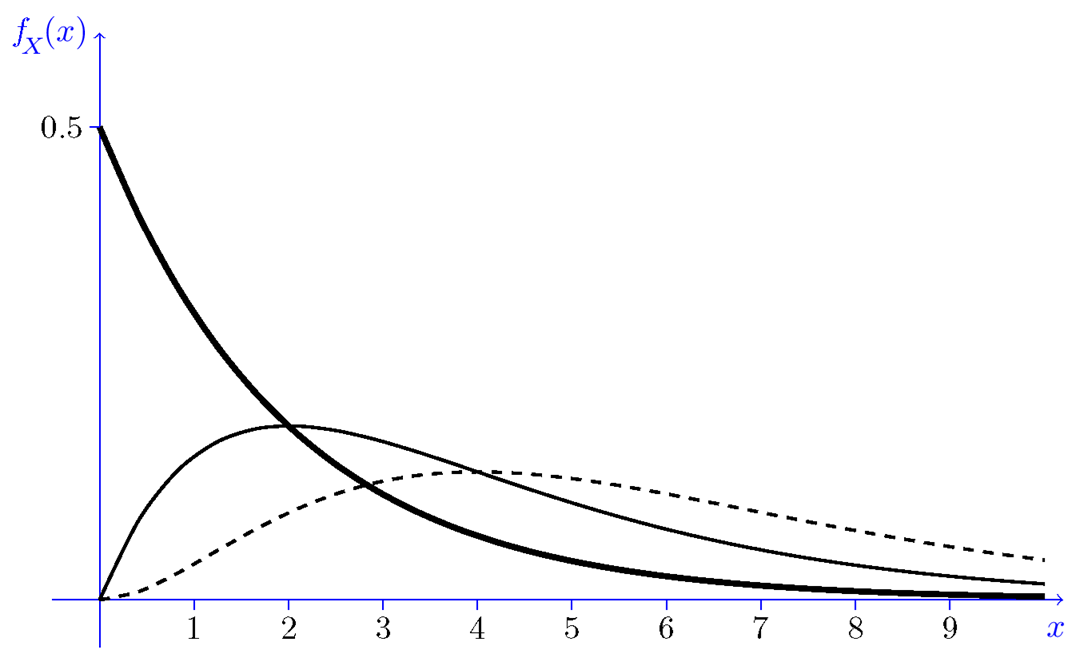
\includegraphics[width=0.8\linewidth]{chapters/chapter 9/PDF graph.png}
    \caption*{երեք տարբեր հնարավոր {\rm PDF}-ներ՝ կախված ճանճի ճաշակից}
\end{figure}

\question{{\it PDF}-ներից յուրաքանչյուրի դեպքում ո՞ր միջակայքում է ամենահավանական, որ ճանճը կնստի։}

Ինչպես դիսկրետ պատահական մեծության դեպքում {\rm PMF}-ին, այնպես էլ անընդհատ պատահական մեծության դեպքում՝ նրա {\rm PDF}-ին նայելով կարող ենք ստանալ բազմաթիվ տեղեկություններ նրա հնարավոր արժեքների ու դրանց հավանականությունների մասին։ 

Օրինակ՝ վերևի գրաֆիկներից յուրաքանչյուրում խտության ֆունկցիան $0$-ից ձախ և $10$-ից աջ զրո է, հետևաբար եթե չիմանայինք էլ՝ նայելով կհասկանայինք, որ $X$-ի հնարավոր արժեքները $[0, 10]$-ն են։ Կարող ենք նաև ասել, որ եթե $f_X$-ի արժեքը մեծ է օրինակ՝ $x=2$ կետում, ապա $X$-ը մեծ հավանականությամբ է արժեքներ ընդունում $2$ կետի հարևան շրջակայքում։ 

Ըստ էության՝ {\rm PDF}-ը {\rm PMF}-ի անալոգն ու փոխարինողն է անընդհատ պատահական մեծությունների համար։ Ինչպես դիսկրետ դեպքում $p_X$-ը, այնպես էլ անընդհատ դեպքում $f_X$-ը չի կարող լինել բացասական՝ 
\[
f_X(x) \ge 0 \qquad \text{ցանկացած $x\in\R$ կետում}
\]
սակայն քանի որ վերջինս հավանականություն չի ցույց տալիս (այլ ընդամենը դրա խտությունը), ապա $f_X$-ը կարող է ընդունել $1$-ից մեծ արժեքներ։ Վերջինիս սահմանումից նաև հետևում է, որ 
\[
\int_{-\infty}^{+\infty} f_X(t)\, dt = F_X(+\infty) = \PP[X \le +\infty] = 1 
\]
քանի որ․․․ ինչպե՞ս կարող է $X$-ը լինել $+\infty$-ից մեծ։

\question{Ունենալով $f_X$-ը՝ ինչպե՞ս գտնել $\PP[a < X < b]$-ն։}

Ամենահաճելի հատկությունը, որի շնորհիվ կարող ենք կիրառել խտության ֆունկցիան՝
\[
\PP[a < X < b] = \int_{a}^{b} f_X(t)\, dt
\]
այսինքն հավանականությունը, որ $X$-ն ընկած է $(a, b)$ միջակայքում հավասար է այդ միջակայքում նրա {\rm PDF}-ի տակ ընկած մակերեսին։

% Նշենք, որ երբեմն անընդհատ պատահական մեծությունները կարող են չունենալ խտություն, բայց 


\section{Հավասարաչափ բաշխում}

Փակենք մեր աչքերն ու մատը դնենք $[0, 10]$ հատվածում որևէ պա\-տա\-հա\-կան $X$ կետի վրա։
Կունենանք մի իրավիճակ, որը շատ նման է ճանճի դեպքին՝ այն տարբերությամբ, որ եթե ճանճը կարող է հակված լինել նստել ավելի ձախ կամ ավելի աջ գտնվող կետերում, և հատ\-վածի տարբեր մասերում նստելու հավանականությունը կարող է տարբեր լինել, ապա\marginnote{նույն երկարությամբ ցանկացած երկու միջակայք նույնչափ հավանական են՝
\[\PP[X \in (1.3, 1.5)] = \PP[X \in (4.7,4.9)]\]} այս օրինակում կարող ենք համարել, որ աչքերը փակ ընտրելիս որևէ նախապատվություն չկա․ ոչ մի թվի մոտ նշելու հավա\-նա\-կա\-նու\-թյունը մյուսից ավել չէ։ 

\question{Ըստ Ձեզ՝ ի՞նչ տեսք կունենա $X$-ի խտության գրաֆիկը։}

$[0, 10]$ հատվածի փոխարեն վերցնենք ավելի ընդհանուր՝ $[a, b]$ հատվածը, և երկրաչափորեն փորձենք պարզել $X$-ի բաշխումը։

Սկսենք {\rm CDF}-ից։ Քանի որ $X$-ի հնարավոր արժեքներն են $[a, b]$, ապա $a$-ից փոքր արժեք ընդունելու հավանականությունը $0$ է՝
\[
F_X(x) = \PP[X \le x] = 0 \qquad \text{եթե } x < a
\]
Պարզենք $F_X(x)$-ի արժեքը, երբ $a \le x \le b$։ 

\begin{center}
\begin{tikzpicture}
    \draw[dashed] (-1.3,0) -- (0,0);
    \draw[-, thick] (0,0) -- (6,0);
    \draw[dashed] (6,0) -- (7.3,0);    
    \draw[thick, myblue] (0,0) -- (4.5,0);
    \foreach \x in {6} {
    \draw[thick] (\x,0.15) -- (\x,-0.15);
    }
    \foreach \x in {0,4.5} {
    \draw[thick, myblue] (\x,0.15) -- (\x,-0.15);
    }
    \node[below, align=center] at (0,-0.15) {$a$};
    \node[below, align=center] at (6,-0.15) {$b$};
    \node[below, align=center] at (4.5,-0.15) {{\color{myblue} $x$}};
\end{tikzpicture}
\end{center}
Հավանականությունը, որ $X$-ը ընկած կլինի $[a, x]$ միջակայքում՝\marginnote{այստեղ արդեն կարող ենք օգտվել երկ\-րա\-չա\-փա\-կան հա\-վա\-նա\-կա\-նու\-թյունից}
\[
F_X(x) = \PP[X \le x] = \frac{\color{myblue} [a, x]\text{-ի երկարություն}}{[a, b]\text{-ի երկարություն}} = \frac{x-a}{b-a}
\]
Դե իսկ եթե $x$-ն ընկած լինի $b$-ից աջ,
\[
F_X(x) = \PP[X \le x] = \PP[X \le b] = 1
\]
և հետևաբար
\[
F_X(x) = \begin{cases}
    0 & \text{եթե } x < a\\
    \dfrac{x-a}{b-a} & \text{եթե } a \le x \le b\\
    1 & \text{եթե } x > b
\end{cases}
\]
Ստացանք $X$-ի բաշխման ֆունկցիան, և եթե այն \marginnote{$a$-ում ու $b$-ում $F_X$-ը ածանցյալ չունի, բայց դրանց կանտեսենք} ածանցենք՝
\[
f_X(x) = \begin{cases}
    \dfrac{1}{b-a} & \text{եթե } a \le x \le b\\
    0 & \text{մնացած կետերում}
\end{cases}
\]
կստանանք նաև $X$-ի խտության ֆունկցիան։

\begin{figure}[h]
    \centering
    \subfloat{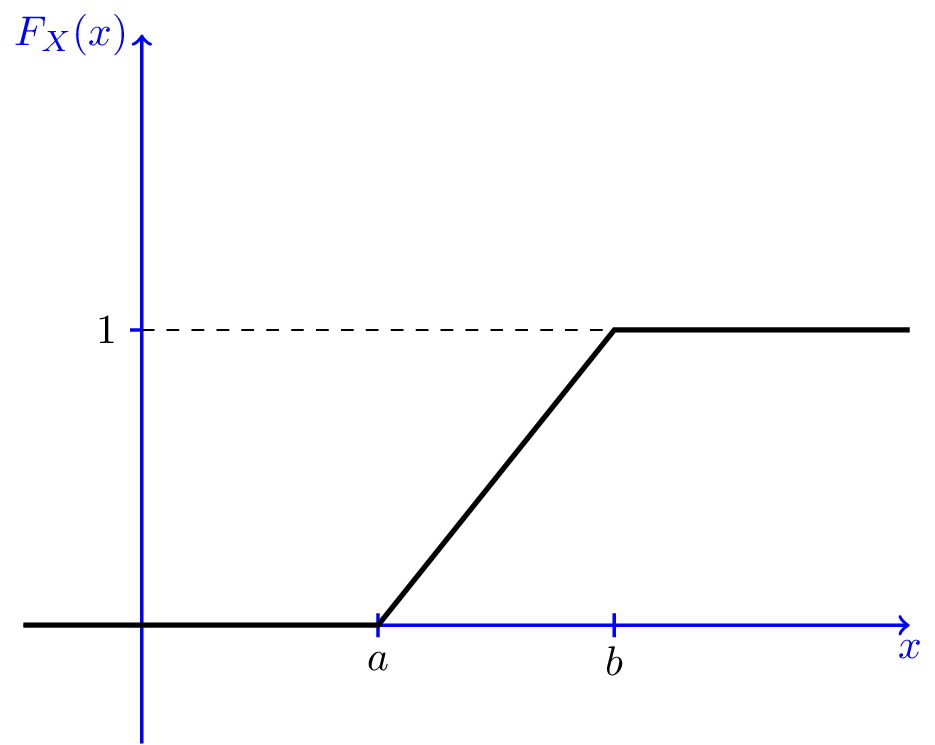
\includegraphics[width=0.4\linewidth]{chapters/chapter 9/uniform CDF.png}}%
    \qquad
    \subfloat{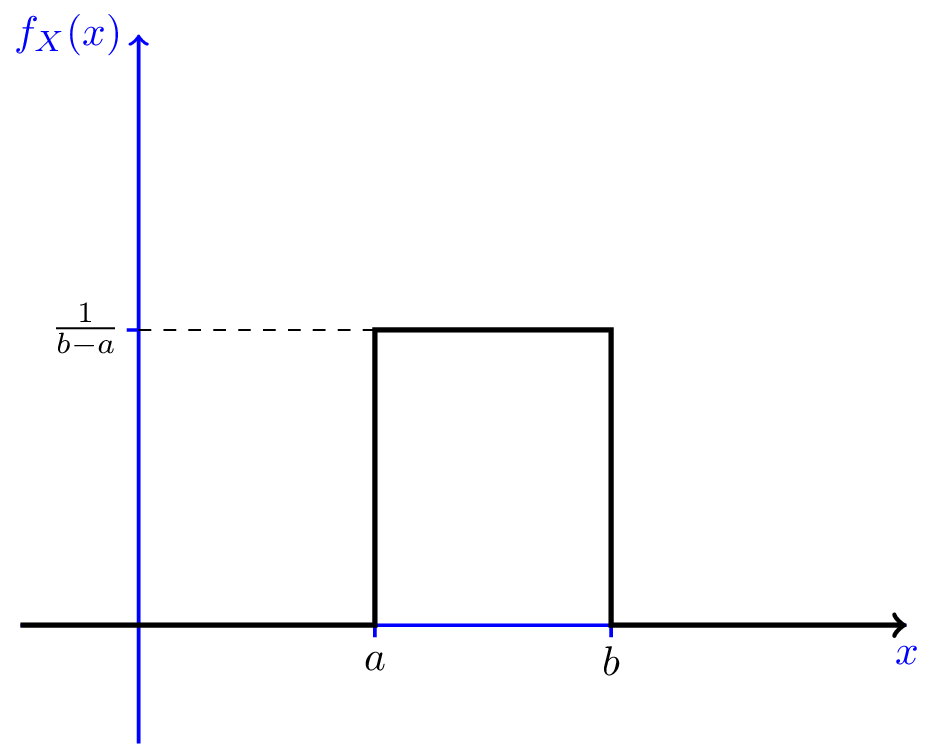
\includegraphics[width=0.4\linewidth]{chapters/chapter 9/uniform PDF.png}} %
\end{figure}

Նկատենք, որ $X$-ի {\rm PDF}-ն ունի մեր ակնկալած տեսքը՝ $[a, b]$-ից դուրս զրո է, իսկ ներսի բոլոր կետերում ընդունում է նույն արժեքը (ուրեմն ոչ մի կետի մոտ հավանականությունը մեծ կամ փոքր չէ), և նրա գրաֆիկի տակ եղած մակերեսը $1$ է։ Մյուս կողմից {\rm CDF}-ը $[a, b]$ միջակայքում գծորեն, այսինքն՝ հաստատուն արագությամբ աճում է։ 
Գրաֆիկների այս տեսքը մատնում է, որ գործ ունենք $[a, b]$-ում արժեքներ ընդունող և բոլորին հավասարապես վերաբերվող պատահական մեծության հետ (որին ժամանակն է անուն տալ)։

\begin{definition}
Կասենք, որ $X$ պատահական մեծությունը \textbf{հավասարաչափ} է բաշխված $(a, b)$ կամ $[a, b]$ \marginnote{անգլերեն՝ {\it uniformly distributed}}միջակայքում՝
\[
X \sim \operatorname{U}(a, b)
\]
եթե 
\[
f_X(x) = \begin{cases}
    \dfrac{1}{b-a} & \text{եթե } a \le x \le b\\
    0 & \text{մնացած կետերում}
\end{cases}
\]
\end{definition}


\section{Անկախություն}

Ենթադրենք նետել ենք երկու զառ։ Նախորդ թեմայում ասացինք, որ զառերի ելքերն իրար հետ կապ չունեն, հետևաբար դրանց հետ կապված ցանկացած երկու պատահույթ անկախ են՝ $\PP[A \cap B] = \PP[A] \cdot \PP[B]$: Մասնավորապես եթե $X$-ով նշենք առաջին զառի թիվը, իսկ $Y$-ով՝ երկրորդինը, ցանկացած $a$ ու $b$ թվերի համար կունենանք
\[
\PP[(X = a) \text{ և } (Y = b)] = \PP[X = a] \cdot \PP[Y = b]
\]
Նույն կերպ, եթե $X$-ով նշանակեինք առաջին զառի թվի քառակուսին, իսկ $Y$-ով ասենք՝ երկրորդի թվի մնացորդը $2$-ի բաժանելիս, միևնույն է դրանց համար այս երկու $\{X=a\}$ և $\{Y=b\}$ պատահույթները լինելու էին անկախ և դրանց \textit{համատեղ} {\rm PDF}-ը՝
\[
\PP[(X = a) \text{ և } (Y = b)]
\]
գրելու էինք արտադրյալով։ 
Տրամաբանական կլինի, եթե այս դեպքում նույնպես ասենք, որ $X$-ն ու $Y$-ը անկախ են։

\begin{definition}
$X$ և $Y$ դիսկրետ պատահական մեծությունները կոչվում են \textbf{անկախ,} եթե ցանկացած $a$, $b\in \R$ թվերի համար
\[
\PP[(X = a) \text{ և } (Y = b)] = \PP[X = a] \cdot \PP[Y = b]
\]
\end{definition}

Իհարկե, անընդհատ պատահական մեծությունների համար բոլոր այս երեք հավանականություններն էլ զրո են, հետևաբար ընդհանուր դեպքում անկախությունը կսահմանենք {\rm CDF}-ների միջոցով՝
\begin{definition}
$X$ և $Y$ պատահական մեծությունները կոչվում են\marginnote{և դիսկրետ, և անընդհատ դեպքում} \textbf{անկախ,} եթե ցանկացած $a$, $b\in \R$ թվերի համար
\[
\PP[(X \le a) \text{ և } (Y \le b)] = \PP[X \le a] \cdot \PP[Y \le b]
\]
\end{definition}

Մասնավորապես, եթե նետենք երկու զառ կամ մետաղադրամ (կամ ցանկացած նման պատահական փորձ կրկնենք երկու անգամ), և ստացվածները նշանակենք $X_1$-ով ու $X_2$-ով, դրանք կլինեն անկախ և միատեսակ բաշխված պատահական \marginnote{առաջին տառերով՝ {\rm i.i.d.}} մեծություններ։



\bigskip 

\begin{theory}
.
\begin{itemize}
\item կարդալ [{\rm Blitzstein-Hwang}], 91-94 (պատահական մեծու\-թյուն), 94-99 ({\rm PMF}), 108-109 ({\rm CDF}), 117-119 (անկախու\-թյուն), 195-197 ({\rm PDF}), 201-202 էջերը 
\item տեսնել պատահական մեծությունների տարբեր \href{https://dlsun.github.io/skis/continuous/random-variables.html}{օրինակներ}
\item դիտել {\aroff PMF, CDF, PDF}-ի մասին օգտակար \href{https://www.youtu.be/yRbfLlTmPE8
}{տեսանյութ}
\item ըստ ցանկության՝ նաև մեկ այլ \href{https://youtu.be/IaSGqQa5O-M}{տեսանյութ} {\rm 3b1b}-ից
\end{itemize}
\end{theory}

\newpage

\section{Խնդիրներ}

\begin{problem}
Երկու անգամ նետում ենք զառը և նշանակում
\begin{align*}
X &= 1\text{-ին զառի թիվը} \\
Y &= 2\text{-րդ զառի թիվը} \\
Z &= \text{այդ երկուսից մեծագույնը} = \max\{X, Y\} 
\end{align*}
Կարո՞ղ եք գտնել $Z$-ի {\rm PDF}-ն ու {\rm CDF}-ը։
\end{problem}

\begin{problem}
Անին պատրաստեց մի արտասովոր զառ ($1$-$6$ թվերով), որի
\begin{itemize}
    \item զույգ ընկնելու հավանականությունը նույնն է, ինչ կենտ ընկնելունը
    \item բոլոր զույգ թվերի հավանականությունները նույնն են
    \item $1$ ընկնելու հավանականությունը $0.5$ է
\end{itemize}
Ի՞նչ տեսք ունի զառի ընկած թվի {\rm PMF}-ը։
\end{problem}

\begin{problem}
$10$ սմ երկարությամբ փայտը երկու պատահական կետերից կտրելով՝ բաժանում են $3$ կտորի։ Որքա՞ն է հավանական, որ այդ երեք կտորներով կարելի է կառուցել եռանկյուն։

\hint{Առաջին երկու կտորները նշանակենք $X$ և $Y$-ով։ Որքա՞ն կլինի երրորդ կտորը։ Եռանկյան համար անհրաժեշտ է, որ կող\-մերից ցանկացած երկուսի գումարը մեծ լինի երրորդից։}
\end{problem}

\begin{problem}\marginnote[*+0.5]{\href{https://www.youtu.be/ccNSU_TsUnQ}{լուծում}}
$(0, 10)$ միջակայքից պատահականորեն վերցնում են երեք թիվ՝
\[
X,\ Y,\ Z \sim \operatorname{U}(0, 10)
\]
իրարից անկախ և հավասարաչափ բաշխված։

Որքա՞ն է հավանականությունը, որ ստացված երկարությամբ հատված\-ներով կարելի է կառուցել եռանկյուն։
\end{problem}

\begin{problem}
$X$ պատահական մեծության խտության ֆունկցիան է՝
\[
f_X(x) = \begin{cases}
    ax^5& \text{եթե }0\le x \le 3 \\
    0& \text{մնացած դեպքերում}
\end{cases}
\]
որտեղ $a$ հաստատունի արժեքն անհայտ է։ Կարո՞ղ եք գտնել $a$-ն։
\end{problem}

\begin{problem}
Համակարգիչը գեներացնում է պատահական թվեր, ընդ որում գեներացված $X$ թվի խտության ֆունկցիան է՝
\[
f_X(x) = \begin{cases}
    1 - |x-1|& \text{եթե }0\le x \le 2 \\
    0& \text{մնացած դեպքերում}
\end{cases}
\]
Գևորգը որոշում է գեներացնել պատահական թիվ և $1$-ից մեծ թվի դեպքում գնալ զբոսնելու, փոքր թվի դեպքում՝ քնելու, իսկ $1$ թվի դեպքում՝ դաս անելու։ Պարզեք, թե
\begin{enumerate}
\item ո՞րն է $X$-ի {\rm CDF}-ը
\item որքա՞ն է հավանական, որ Գևորգը կգնա զբոսնելու
\item որքա՞ն է հավանական, որ Գևորգը դաս չի անի
\end{enumerate}
\end{problem}

\begin{problem}
Վերոնշյալ մարտավարության արդյունքում հավտեսի \marginnote[*-0.5]{\textit{հավ}անականությունների \textit{տես}ության} քննությանը Գևորգի պատասխանած հարցերի տոկոսը ցույց տվող $X$ պատահական մեծության բաշխման ֆունկցիան է՝
\[
F_X(x) = \begin{cases}
    0& \text{եթե } x < 0 \\
    \sqrt{x}& \text{եթե } 0 \le x \le 1 \\
    1& \text{եթե } x > 1
\end{cases}
\]
Որքա՞ն է հավանականությունը, որ Գևորգը ճիշտ կպատասխանի հար\-ցերի գոնե կեսին։  
\end{problem}
\setchapterpreamble[u]{\margintoc}
\chapter{Վիճակագրական բնութագրիչներ}
\labch{descriptors}

\emergencystretch 2em

\section{Մաթսպասում}

Խաղում ենք հետևյալ խաղը։ Ամեն անգամ ընտրում ենք $1$-$38$ թվերից որևէ մեկը (ենթադրենք՝ $8$), կատարում ենք $\$1$-ի խաղադրույք, պտտում ռուլետկան և
\begin{itemize}
    \item եթե ընկնում է $8$, ապա շահում ենք $\$36$
    \item հակառակ դեպքում՝ կորցնում $\$1$-ը
\end{itemize}

\question{Կխաղայի՞ք արդյոք այսպիսի խաղ։}

Հավանաբար կպատասխանեք, որ ոչ, քանի որ հաղթելու հավանակա\-նու\-թյունը շատ փոքր է, իսկ շահելու ենթակա գումարը՝ ոչ այնքան մեծ։ 


\begin{marginfigure}
    \centering
    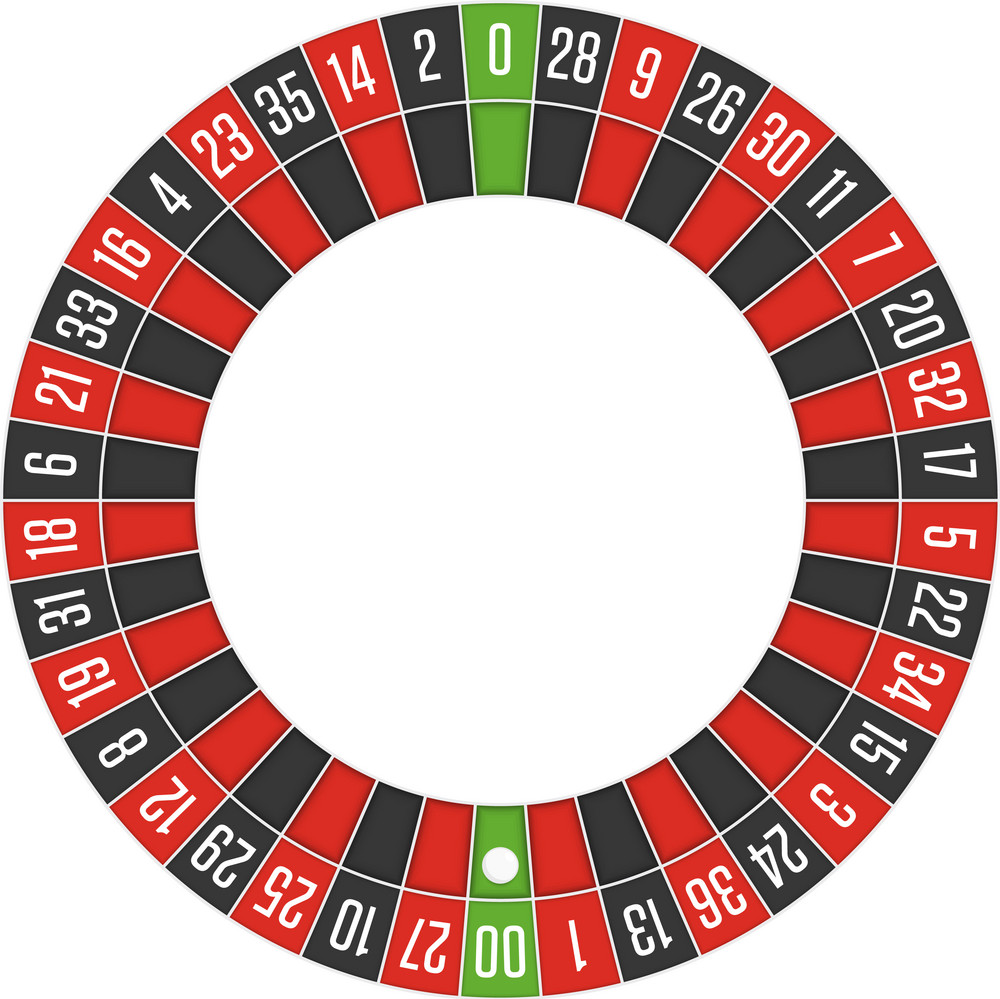
\includegraphics[width=0.8\linewidth]{chapters/chapter 10/roulette.png}
\end{marginfigure}

\question{Իսկ եթե $8$ ընկնելու դեպքում շահեիք $\$150$՞։ Իսկ $\$37.01$-ի դեպքո՞ւմ։}

Քանի որ հաղթելու հավանականությունն ընդամենը $\dfrac{1}{38}$ է, ապա կոպիտ ասած՝ եթե $38\,000$ անգամ պտտենք, $1000$ անգամը կընկնի մեր պահած թիվը, արդյունքում կշահենք
\[
1000 \cdot \color{mygreen}37.01
\]
իսկ մնացած անգամները՝ կկորցնենք
\[
37000 \cdot \color{myred}(-1)
\]
Ուրեմն ընդհանուր առմամբ $38\,000$ անգամ խաղալով կունենանք մոտ
\[
1000 \cdot 37.01 + 37000 \cdot (-1) = 10
\]
դոլարի շահույթ, կամ միջինում ամեն մի խաղում՝
\[
\frac{1000}{38000} \cdot 37.01 + \frac{37000}{38000} \cdot (-1) = \frac{10}{38000}
\]
այսինքն՝ $\approx \$0.0003$ շահույթ։ 

Այս թիվը իհարկե մեծ չէ, բայց դրական է․ եթե այս խաղը խաղանք մի քանի միլիարդ անգամ, կարող ենք միլիոնների շահույթ ակնկալել։ Բնականաբար, հնարավոր է՝ բախտներս չբերի, մեր սպասածից քիչ տանենք, կամ էլ հակառակը՝ բախտի բերմամբ հաջողվի շատ գումար տանել, բայց միջինում կարող ենք \textit{սպասել} ամեն խաղից մոտ $\approx \$0.0003$-ի շահույթ։ 

\begin{definition}
$X$ դիսկրետ պատահական մեծության \textbf{մաթսպա\-սում}\marginnote{անգլերեն՝ {\it expected value}} կանվանենք
\[
\E[X] =  \sum_{x_k} x_k\cdot \PP[X=x_k] 
\]
թիվը։
\end{definition}

Այսինքն՝ հերթով կդիտարկենք $X$ պատահական մեծության բոլոր հնա\-րավոր $x_k$ արժեքները և կվերցնենք դրանց \textit{կշռավորված միջինը՝}
\[
\E[X] = \sum_{X\text{-ի արժեքները}} \overbrace{x_k}^{\text{ամեն արժեք}}\cdot \underbrace{\PP[X=x_k]}_{\text{իր հավանականությամբ}}
\]
Մասնավորապես եթե $X$-ի բոլոր արժեքներն ունեն նույն հավանականու\-թյունը, $\E[X]$-ը կլինի այդ արժեքների միջին թվաբանականը, իսկ եթե օրինակ՝ արժեքներից մեկը $100$ անգամ ավելի հավանական է, քան մյուսը, ապա $\E[X]$-ը հաշվելիս այն կունենա $100$ անգամ ավելի մեծ կշիռ։

\question{Եթե նետենք մետաղադրամն ու գիր ընկնելու դեպքում վերցնենք $X=1$, ղուշի դեպքում՝ $X=0$, որքա՞ն կլինի $\E[X]$-ը։}

\begin{example}\label{die_rv}
Նետում ենք զառն ու $X$-ով նշանակում ընկած թիվը։ Այդ դեպքում $X$-ի մաթսպասումը կլինի՝
\[
\E[X] = \frac{1}{6} \cdot 1 + \frac{1}{6} \cdot 2 + \dots + \frac{1}{6} \cdot 6 = \frac{1+2+\dots+6}{6} = \frac{7}{2} %3.5
\]
այսինքն բոլոր արժեքների միջինը։ 
\end{example}

Իսկ եթե ուզեինք պարզել $X^2$ արտահայտության \marginnote{$X^2$-ն \hyperref[transformed_rv]{\color{OliveGreen} ևս} պատահական մեծություն է}միջինը, պարզապես կվերցնեինք $X$-ի արժեքների քառակուսիներն ու կրկին կբազմապատ\-կե\-ինք այդ արժեքների հավանականություններով՝
\[
\E[X^{\color{myred} 2}] = \frac{1}{6} \cdot 1^{\color{myred} 2} + \frac{1}{6} \cdot 2^{\color{myred} 2} + \dots + \frac{1}{6} \cdot 6^{\color{myred} 2} = \frac{1^{\color{myred} 2}+2^{\color{myred} 2}+\dots+6^{\color{myred} 2}}{6} = \frac{91}{6} %\approx 15.17
\]

\warning{Ինչպես տեսնում ենք, $\E[X^2] \ne \E[X]^2$:}

Նույնը նաև $X^3$-ի, $\dfrac{1}{X}$-ի, $\cos(X)$-ի և առհասարակ ցանկացած $g(X)$ տեսքի պատահական մեծության համար՝\marginnote{այս կանոնը \href{https://en.wikipedia.org/wiki/Law_of_the_unconscious_statistician#Etymology}{անվանում են} {\rm LOTUS}}
\[
\E[g(X)] =  \sum_{x_k} g(x_k)\cdot \PP[X=x_k] 
\]
Եկեք հիմա սահմանենք մաթսպասման գաղափարը անընդհատ պա\-տա\-հական մեծության համար։ Քանի որ անընդհատ $X$-ի դեպքում նրա ցանկացած արժեք ընդունելու հավանականությունը $0$ է, $\PP[X=x_k]$-ն փոխարինենք իր անընդհատ անալոգով՝ $f_X(x)$ խտությամբ, իսկ քանի որ միջակայքում ընկած բոլոր թվերը չենք կարող գումարել, $\sum$ գումարի նշանը փոխարինենք ինտեգրալով՝
\begin{align*}
\PP[X=x] &\mapsto f_X(x) \\
\sum_{X\text{-ի արժեքները}} &\mapsto \int_{a}^{b}
\end{align*}
որտեղ $(a, b)$-ն այն միջակայքն է, որին պատկանում են $X$-ի բոլոր հնարավոր արժեքները։ \marginnote{$(a, b)$-ն այն $x$-երն են, որտեղ $f_X(x) \ne 0$} 
Ցանկության դեպքում կարող ենք իհարկե ինտեգրել ոչ թե միայն $(a, b)$ միջակայքի, այլ ողջ առանցքի երկայնքով՝ $(-\infty, \infty)$, բայց քանի որ $(a, b)$-ից դուրս $f_X(x)$-ը զրո է, ապա դա նույնը կլինի, ինչ ինտեգրել $(a, b)$-ով։ Ուրեմն,

\begin{definition}
$X$ անընդհատ պատահական մեծության \textbf{մաթ\-սպա\-սում} կանվանենք
\[
\E[X] = \int_{-\infty}^{+\infty} x \cdot f_X(x) \, dx
\]
թիվը։
\end{definition}
Կրկին այն միջակայքերը, որոնցում խտության ֆունկցիան ավելի մեծ է, կունենան ավելի շատ կշիռ, քան ավելի ցածր խտությամբ միջա\-կայքերը։ 

\begin{example}\label{metro}
Գագիկն ամեն օր «Բարեկամությունից» դասի գնալիս չափում է, թե նախատեսվածից քանի րոպե ուշ կամ շուտ է շարժվում մետրոն։ Չափումների շնորհիվ նա պարզել է, որ այդ րոպեների տարբերությունը ցույց տվող պատահական մեծության {\rm PDF}-ն է՝
\[
f_X(x) = e^{-x^2}
\]

\begin{marginfigure}
    \centering
    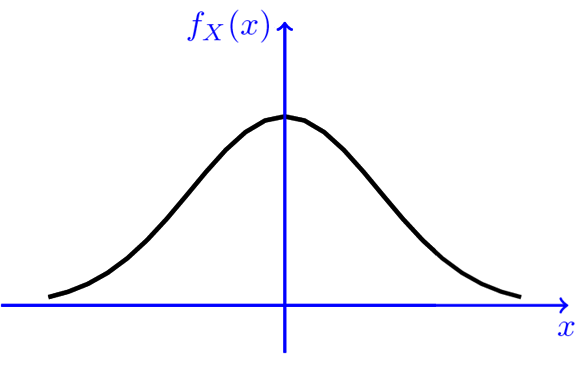
\includegraphics[width=\linewidth]{chapters/chapter 10/normal PDF.png}
    \caption*{$x$-երի առանցքը րոպեներն են}
\end{marginfigure}

Սկզբում փորձեք $f_X$-ի գրաֆիկին նայելով կռահել, թե միջինում քանի՞ րոպե է ուշանում մետրոն, ապա այն ճշգրիտ կհաշվենք։ 

Գրենք $\E[X]$-ը հետևյալ տեսքով և ինտեգրենք՝
\begin{align*}
\E[X]
= \int_{-\infty}^{+\infty} xe^{-x^2}\, dx
&= \frac{1}{2}\int_{-\infty}^{+\infty} e^{-x^2}(x^2)'\, dx \\
&= \frac{1}{2}\int_{-\infty}^{+\infty} e^{-x^2} d(x^2)
= \frac{1}{2} \left.e^{-x^2}\right|_{x=-\infty}^{+\infty} = 0
\end{align*}
Ուրեմն թեև որոշ օրերի մետրոն շուտ է շարժվում, որոշ օրերի՝ ուշ, միջինում այն շարժվում է․․․ ճիշտ ժամանակին։
\end{example}

Նման ձևով կարող ենք նաև $X$-ը դնել ցանկացած $g$ անընդհատ ֆունկցիայի մեջ և հաշվել $g(X)$-ի մաթսպասումը՝
\[
\E[g(X)] = \int_{-\infty}^{+\infty} g(x) \cdot f_X(x) \, dx
\]
\question{$X$-ը ի՞նչ ֆունկցիայի մեջ պետք է դներ Գագիկը, որպեսզի $\E[g(X)]$-ը ցույց տար միջինում մետրոյի շեղումը ժամացուցակից։}

Ենթադրենք հայտնի է, որ միջինում ամեն մեծահասակ մարդու համար ծախսվում է օրական $2500$ դրամ, իսկ ամեն երեխայի համար՝ $4000$ դրամ։

\question{Օրական միջինում որքա՞ն է ծախսում $1$ մեծից և $1$ երեխայից կազմված ընտանիքը։ Իսկ $2$ մեծից և $3$ երեխայի՞ց։}

Ինչպես տրամաբանորեն պետք է լիներ, \marginnote[*+3]{ավելի ընդհանուր՝ \[\E[X_1+X_2+\dots] = \E[X_1] + \E[X_2] + \dots\]}
\begin{align*}
\E[c \cdot X] &= c \cdot \E[X] \\
\E[X + c] &= \E[X] + c \\
\E[X + Y] &= \E[X] + \E[Y]
\end{align*}
և եթե մի պատահական մեծություն միշտ փոքր/հավասար է մյուսից՝ $X \le Y$, ապա $\E[X] \le \E[Y]$:

Իսկ ի՞նչ կարելի է ասել պատահական մեծությունների \textit{արտադրյալի} մաթսպասման մասին։ Պարզվում է, որ
\begin{theorem}\label{independence_E}
Եթե $X$-ն ու $Y$-ն անկախ են, ապա
\[
\E[X \cdot Y] = \E[X] \cdot \E[Y]
\]
\end{theorem}

\warning{Հակառակը ոչ միշտ է ճիշտ․ եթե $\E[XY] = \E[X] \cdot \E[Y]$, դա դեռ չի նշանակում, որ $X$-ն ու $Y$-ն անկախ են։}


\section{Վարիացիա}

Նկարում պատկերված են երկու տարբեր ընկերություններում աշխա\-տա\-վարձերի խտության գրաֆիկները:\marginnote{$=$ պատահական վերցված աշխատակցի աշխատավարձի {\rm PDF}-ը} Ինչպես տեսնում ենք, երկուսում էլ միջին աշխատավարձը $200\,000$ դրամ է, սակայն 
\begin{itemize}
    \item հիմնարկներից մեկում աշխատավարձերը մոտ են իրենց միջինին
    \item մյուսում՝ միջինից բավական հեռու են, ցրված են
\end{itemize}

\begin{figure}[b]
    \centering
    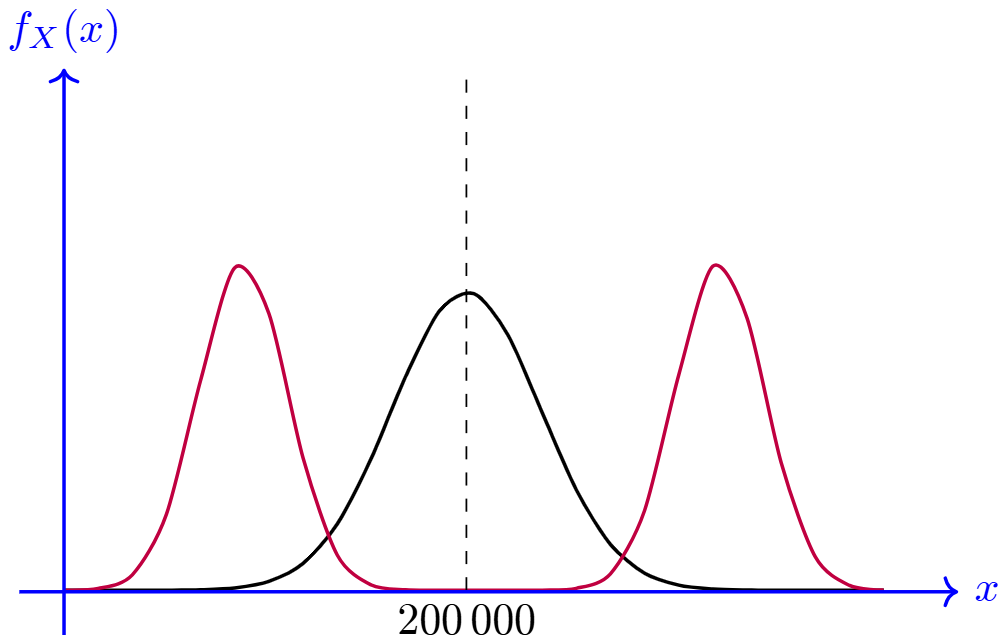
\includegraphics[width=0.65\linewidth]{chapters/chapter 10/salaries.png}
\end{figure}


% \begin{tikzpicture}[scale=1.2]
%   \draw[domain=0:5.5, smooth, variable=\x, thick]
%     plot ({\x}, {2*exp(-((\x - 2.7)^2)/(2*0.5^2))});

%   \draw[domain=0:5.5, smooth, variable=\x, thick, purple]
%     plot ({\x}, {
%       2.2*exp(-((\x - 1.2)^2)/(2*0.3^2)) +
%       2.2*exp(-((\x - 4.4)^2)/(2*0.3^2))
%     });
  
%   \draw[dashed] (2.7,0) -- (2.7,3.5);
%   \node[below] at (2.7,0) {$200\,000$};
%   \draw[->, thick, blue] (-0.3,-0.01) -- (6,-0.01) node[anchor=west] {\textcolor{blue}{$x$}};
%   \draw[->, thick, blue] (0,-0.3) -- (0,3.5) node[anchor=south] {\textcolor{blue}{$f_X(x)$}};
% \end{tikzpicture}

Ինչպե՞ս չափենք միջինից ունեցած այս շեղումը՝ $X$-ի արժեքների և $\E[X]$-ի հեռավորությունը։ Սկզբի համար կարող ենք յուրաքանչյուր աշխատակցի $X$ աշխատավարձից հանել այդ միջինը՝
\[
X - \E[X]
\]
Երկրաչափորեն սա կնշանակի $f_X$-ի գրաֆիկը $\E[X]$-ով տանել ձախ, այսինքն այնպես, որ ստացվածի միջինը լինի $0$։

Այն աշխատակիցների համար, որոնք ստանում էին միջինից բարձր աշխատավարձ՝ $X > \E[X]$, այս մեծությունը կլինի դրական, մյուսների համար՝ բացասական։ Թեև մեզ հարկավոր է այդ շեղումների միջինը, բայց եթե վերցնենք ստացվածի մաթսպասումը՝
\[
\E[X - \E[X]]
\]
շատ ստացողների դրական շեղումը կկրճատվի քիչ ստացողների բա\-ցա\-սական շեղման հետ, և հնարավոր է՝ ստանանք $0$, ինչպես \hyperref[metro]{\color{OliveGreen} մետրոյի} օրինակում։ Ուրեմն դարձնենք այս տարբերությունը դրական։

Տարբերակներից մեկն է վերցնել ստացվածի մոդուլը, ապա հաշվել դրա միջինը՝
\[
\E\left[\left|X - \E[X]\right|\right]
\]
մեկ ուրիշ տարբերակ է մոդուլի փոխարեն բարձրացնել քառակուսի՝
\[
\E\left[\left(X - \E[X]\right)^2\right]
\]

\question{Ո՞րը կընտրեիք Դուք։ Ո՞րը երբ պետք կգա։}

\begin{example}
Ենթադրենք $X$-ը ինչ-որ պատահական մեծություն է, որն ընդունում է երեք արժեք՝ $0$, $10$ և $15$, հետևյալ հավանականություն\-նե\-րով՝
\[
\PP[X = 0] = 0.6, \qquad \PP[X = 10] = \PP[X = 15] = 0.2
\]
Անշուշտ, $X$-ի արժեքներն իրենց միջինից՝
\[
\E[X] = 0 \cdot 0.6 + 10 \cdot 0.2 + 15 \cdot 0.2 = 5
\]
բավականին շեղված են։ Շեղման չափը՝ $X-\E[X]$-ը, $0.6$ հավանակա\-նու\-թյամբ հավասար է $-5$, $0.2$-ով՝ $5$, $0.2$-ով՝ $15$, հետևաբար\marginnote[*+1]{ինքնուրույն ստուգեք սա}
\[
\E\left[\left|X - \E[X]\right|\right]
= 
0.6 \cdot |-5| + 0.2 \cdot |5| + 0.2 \cdot |15|
=
7
\]
իսկ 
\[
\E\left[\left(X - \E[X]\right)^2\right]
=
0.6 \cdot (-5)^2 + 0.2 \cdot 5^2 + 0.2 \cdot 15^2
= 
65
\]
Այժմ $X$-ի արժեքներից մեկը $1$ միավորով մոտեցնենք միջինին, մյուսը՝ նույնքան հեռացնենք, և ստացվածը նշանակենք $Y$-ով․
\[
\PP[Y = 0] = 0.6, \qquad \PP[Y = 9] = \PP[Y = 16] = 0.2
\]
Այս գործողությունը անելիս մաթսպասումը չի փոխվի՝ $\E[Y]=\E[X]=5$, իսկ արժեքների հեռավորությունները $\E[Y]$-ից
\begin{itemize}
\item մոդուլով հաշվելու դեպքում կմնա նույնը․
\[
\E\left[\left|Y - \E[Y]\right|\right]
=
0.6 \cdot |-5| + 0.2 \cdot |4| + 0.2 \cdot |16|
= 
1
\]
\item քառակուսիով հաշվելու դեպքում՝ կմեծանա․
\[
\E\left[\left(Y - \E[Y]\right)^2\right]
=
0.6 \cdot (-5)^2 + 0.2 \cdot 4^2 + 0.2 \cdot 16^2
= 
69.4
\]
\end{itemize}

Եթե արժեքները ևս $1$-ով բրդենք համապատասխանաբար ձախ ու աջ՝
\[
\PP[Z = 0] = 0.6, \qquad \PP[Y = 8] = \PP[Y = 17] = 0.2
\]
մաթսպասումն ու մոդուլով հեռավորությունը նորից կմնան նույնը, իսկ քառակուսիովը՝ կրկին կմեծանա․
\[
\E\left[\left(Z - \E[Z]\right)^2\right]
=
0.6 \cdot (-5)^2 + 0.2 \cdot 3^2 + 0.2 \cdot 17^2
= 
74.6
\] 
և այդպես շարունակ․ չնայած մեր պատահական մեծության որոշ ար\-ժեք\-ներ ավելի ու ավելի են հեռանում միջինից, մոդուլով հեռա\-վո\-րու\-թյունն այդ ցրվածությունը չի ֆիքսում, իսկ քառակուսով հե\-ռա\-վո\-րու\-թյունը՝ գնալով ավելի մեծ թվեր է վերադարձնում։
\end{example}

Պատճառն, իհարկե, քառակուսին է․ որքան մեծ է ինչ-որ արժեքի շեղումը, այնքան ավելի մեծ է նրա քառակուսին։ Ավելի պատկերավոր օրինակ՝

\begin{example}
Ձեզ պետք է արյան ճնշումը $10$ մմ ս․ս․-ով բարձրացնել։ Դեղատանն առաջարկում են երկու դեղ՝
\begin{itemize}
\item մեկը խմելիս ճնշումը կբարձրանա $X$-ով, ընդ որում
\[
\hspace{-2em}\PP[X=8.75] = 0.6, \qquad \PP[X=10.5] = 0.3, \qquad \PP[X=16] = 0.1
\]
\item մյուսի դեպքում՝ $Y$-ով, ընդ որում
\[
\hspace{-2em}\PP[Y=6.8] = 0.25, \qquad \PP[Y=10] = 0.7, \qquad \PP[Y=26] = 0.05
\]
\end{itemize}
Ո՞ր դեղը կնախընտրեք խմել։
Եթե վաճառողին հարցնեք, թե ո՞րն է ավելի վստահելի, նա կպատասխանի, որ երկու դեղերն էլ նույնն են՝ միջինում ազդեցությունը $10$ է, մոդուլով միջին շեղման չափը՝ $1.6$։ 

Մինչդեռ եթե հարցնեք դրանց միջին քառակուսային շեղումները՝\marginnote{ավելի ճշգրիտ՝ շեղման քառակուսիները}
\begin{align*}
\E\left[\left(X - \E[X]\right)^2\right] &= 1.25^2 \cdot 0.6 + 0.5^2 \cdot 0.3 + 6^2 \cdot 0.1 \approx 4.6\\
\E\left[\left(Y - \E[Y]\right)^2\right] &= 3.2^2 \cdot 0.25 + 0^2 \cdot 0.7 + 16^2 \cdot 0.05 \approx 15.4
\end{align*}
կտեսնեք, որ երկրորդի շեղումն անհամեմատ ավելի մեծ է, այսինքն՝ երկրորդն ավելի \textit{ռիսկային} է։
\end{example}

Իրոք, այն փաստը, որ $5\%$ հավանականություն կա, որ արյան ճնշումը $10$-ի փոխարեն $26$-ով կբարձրանա, որևէ ձևով չի արտացոլվում մոդուլով շեղման մեջ, իսկ քառակուսիով հաշվելիս զգացվում է։ Հետևաբար երկրորդ տարբերակով շեղման չափը հաշվելն ավելի պիտանի է ռիսկերը գնահատելու տեսանկյունից։ 

\begin{definition}
$X$ պատահական մեծության ցրվածք կամ \textbf{վարիացիա} կանվանենք\marginnote{անգլերեն՝ {\it variance}} 
\[
\Var[X] = \E\left[\left(X - \E[X]\right)^2\right] 
\]
թիվը, իսկ դրա արմատը կանվանենք \marginnote{{\it standard deviation}}\textbf{ստանդարտ շեղում:}
\end{definition}

Ինչպես տեսանք վերևում և ինչպես երևում է բանաձևից, վարիացիան ցույց է տալիս, թե միջինում պատահական մեծության արժեքները որքանով են հեռու իրենց միջինից։ Քանի որ այդ հեռավորությունը \marginnote{ինչ-որ իմաստով՝ $\Var[X]$-ը $X$-ի ու $\E[X]$-ի $\operatorname{L}_2$ հեռավորության քառա\-կու\-սին է ($\approx$ $X$-ի նորմի քառակուսին)} հաշվելիս շեղումները քառակուսի ենք բարձրանում, ապա նոր «միջի\-նաց\-նում», իմաստ ունի ստացված թվի արմատը դիտարկելը․ այդտեղից էլ ստանդարտ շեղման օգտակարությունը։

\warning{Ինչպես $\E[X]$-ը, այդպես էլ $\Var[X]$-ը թվեր են, ոչ թե պատահական մեծություններ։}

Քանի որ այնքան էլ հարմար չէ այս բանաձևով $\Var[X]$-ը հաշվել, փորձենք այն պարզեցնել․\marginnote[*+2]{հաստատունները նշված են {\color{myblue} կապույտով}}
\begin{align*}
\Var[X] 
&= \E\left[\left(X - {\color{myblue}\E[X]}\right)^2\right] 
= \E\left[X^2 - {\color{myblue} 2} \cdot X \cdot {\color{myblue}\E[X]} + {\color{myblue}\E[X]^2} \right] 
\\
&= \E\left[X^2\right] - \E\left[{\color{myblue} 2} \cdot X \cdot {\color{myblue}\E[X]}\right] + {\color{myblue}\E[X]}^2
\\
&= \E\left[X^2\right] - {\color{myblue} 2} \cdot {\color{myblue}\E[X]} \cdot \E\left[X \right] + {\color{myblue}\E[X]}^2 = \E\left[X^2\right] - \E[X]^2
\end{align*}
Ստացանք բավականին հարմար բանաձև՝ $\Var[X] = \E[X^2] - \E[X]^2$:

\begin{example}
\hyperref[die_rv]{\color{OliveGreen} Կրկին} $X$-ով նշանակենք զառը նետելիս ընկնող թիվը։ Այդ թվի վարիացիան կլինի՝
\[
\Var[X] = \E[X^2] - \E[X]^2 = \frac{91}{6} - \left(\frac{7}{2}\right)^2 \approx 2.92
\]
իսկ ստանդարտ շեղումը՝ $\approx 1.71$:
\end{example}

Մինչև առաջ անցնելը նկատենք վարիացիայի մի քանի հատկություններ։ Նախ՝ հեռավորության քառակուսին չի կարող լինել բացասական, ուրեմն
\[
\Var[X] \ge 0
\]
ընդ որում՝ զրոյի հավասար կարող է լինել միայն եթե $X$-ի բոլոր արժեքները նույնն են, այսինքն $X$-ն ընդունում է միայն մեկ արժեք։ 

Ի տարբերություն մաթսպասման՝ երբ պատահական մեծությունը բազմապատկում ենք որևէ թվով, նրա վարիացիան բազմապատկվում է այդ թվի քառակուսիով՝
\[
\Var[c\cdot X] = c^2 \cdot \Var[X]
\]
իսկ արժեքները հաստատունով մեծացնելիս կամ փոքրացնելիս դրանց ցրվածությունը, բնականաբար, չի փոխվում՝
\[
\Var[X + c] = \Var[X]
\]

\warning{Շատ դեպքերում $\Var[X + Y] \ne \Var[X] + \Var[Y]$:}
\question{Ի՞նչ եք կարծում, ե՞րբ կլինի $\Var[X+Y] = \Var[X] + \Var[Y]$:}

Իրոք, սահմանման մեջ առկա քառակուսու պատճառով
\[ 
\Var[X + Y] = \Var[X] + \Var[Y] + 2\left(\E[XY] - \E[X] \cdot \E[Y]\right)
\]
այսինքն՝ \marginnote{ինչպես \textit{ուղղահայաց} $\va$ ու $\vb$-ի դեպքում \[\|\va+\vb\|^2 = \|\va\|^2 + \|\vb\|^2\] այնպես էլ \textit{անկախ} $X$ ու $Y$-ի դեպքում՝ \[\Var[X+Y] = \Var[X] + \Var[Y]\]} գումարի վարիացիան կախված է ոչ միայն առանձին-առանձին գումարելիների վարիացիաներից, այլև դրանց՝ \textit{իրար հետ ունեցած} կապից։
Իսկ երբ $X$-ն ու $Y$-ն անկախ են, $\E[XY]$-ը \hyperref[independence_E]{\color{OliveGreen} հավասար է լինում} $\E[X] \cdot \E[Y]$-ի, և ունենում ենք $\Var[X] + \Var[Y]$։

\section{Կովարիացիա}

Ենթադրենք ունենք երկու պատահական մեծություններ, ասենք՝ «Տեսլա» և «Երազ» ընկերությունների արժեթղթերը։ \marginnote{այսինքն՝ պատահական վերցված օրը որքա՞ն են դրանց արժեքները} Ինչպե՞ս պարզենք, թե որքա\-նով են դրանք իրարից կախված, կամ ավելի կոնկրետ՝ երբ դրան\-ցից մեկը աճում/նվազում է, որքան է փոխվում մյուսը։ 

\begin{figure}[h]
    \centering
    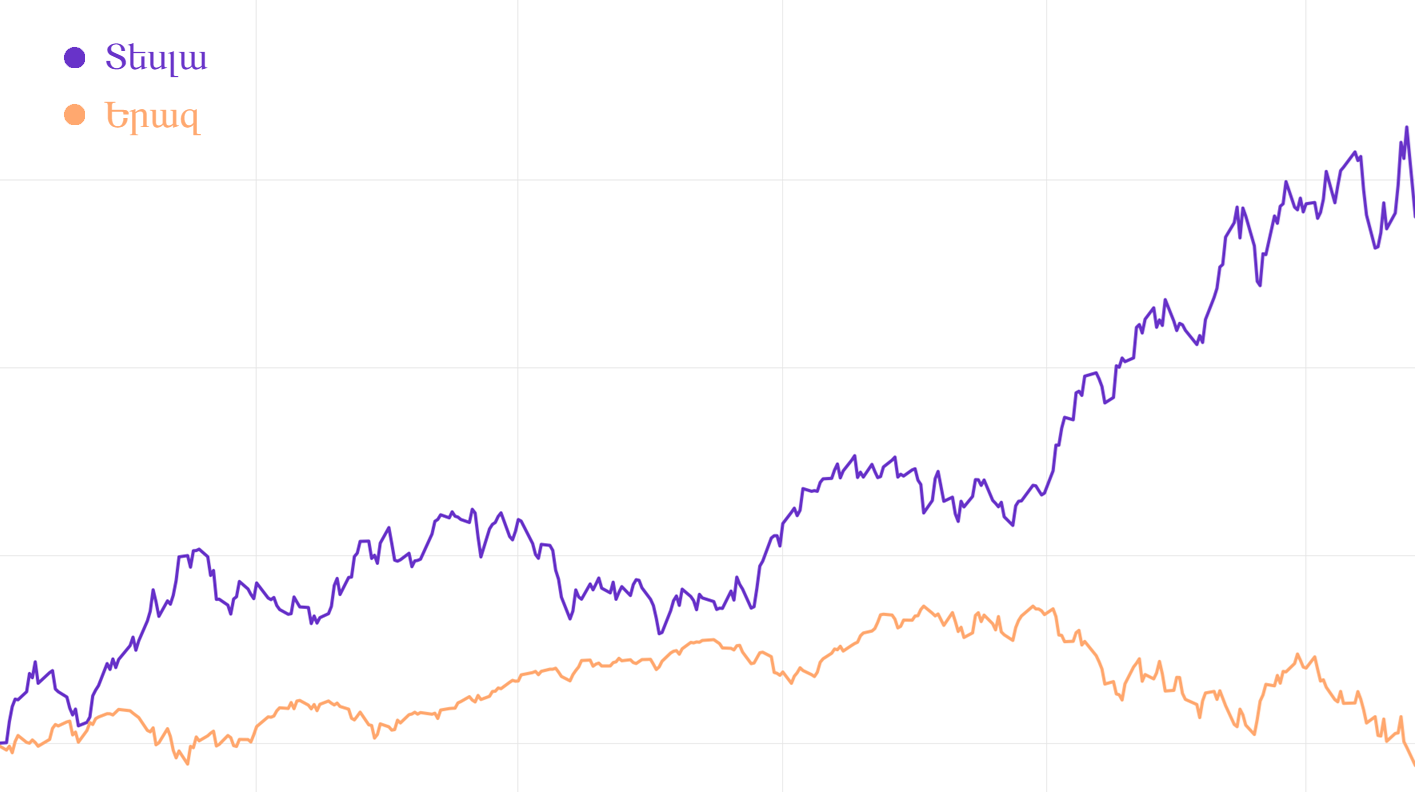
\includegraphics[width=0.65\linewidth]{chapters/chapter 10/stocks.png}
\end{figure}

\question{Ի՞նչ գործիք էինք օգտագործում երկու $\va$ և $\vb$ վեկտորների կապը/նմանությունը չափելու համար։}

Նախ կարող ենք $xy$-հարթության վրա պատկերել $X$-ի և $Y$-ի միաժամանակ ունեցած արժեքների թվազույգերը, տվյալ դեպքում՝ ամեն օրվա համար նշել $(x, y)$ կետը, որտեղ $x$-ն այդ օրը «Տեսլայի» արժեթղթի գինն է, $y$-ը՝ «Երազի»։ 

Խելքին մոտ կլինի նաև, եթե $X$ պատահական մեծության փոփոխության չափ ասելով հասկանանք նրա արժեքների՝ իր միջինի համեմատ ունեցած տարբերությունը՝ $X - \E[X]$, և ներմուծենք մի այսպիսի գործիք․

\begin{definition}
$X$ և $Y$ պատահական մեծությունների \textbf{կովարիա\-ցիա} կանվանենք
\[
\Cov[X, Y] = \E\left[(X-\E[X])(Y-\E[Y])\right]
\]
թիվը։
\end{definition}

Փաստորեն կովարիացիան ցույց է տալիս, թե միջինում որքան է $X$-ի փոփոխության և $Y$-ի փոփոխության արտադրյալը։ Եթե օրինակ՝ $X$-ը (իր միջինի համեմատ) $1$ միավորով\marginnote{գծային հանրահաշվի լեզվով ասած՝ կովարիացիան պատահական մեծու\-թյուն\-ների սկալյար արտադրյալն է} մեծանալիս $Y$-ը (իր միջինի համեմատ) միշտ մեծանա $5$ միավորով, իսկ $X$-ը $1$-ով փոքրանալիս էլ՝ փոքրանա $5$-ով, ապա կունենանք $\Cov[X, Y] = 5$։ 

\newpage

\begin{figure}[t]
\centering %
\floatsetup{floatrowsep=qquad}
\begin{floatrow}[3]%
\ffigbox[\FBwidth]{\caption*{\centering $\Cov[X, Y] > 0$}}{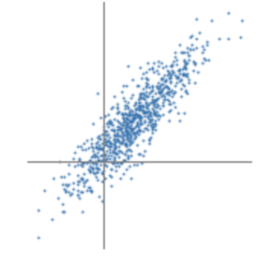
\includegraphics[width=0.4\textwidth]{chapters/chapter 10/covariance 1.png}}
\ffigbox[\FBwidth]{\caption*{\centering $\Cov[X, Y] < 0$}}{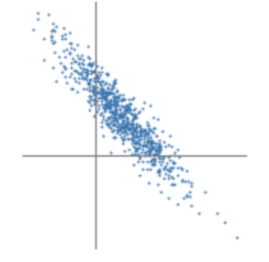
\includegraphics[width=0.4\textwidth]{chapters/chapter 10/covariance 2.png}}
\ffigbox[\FBwidth]{\caption*{\centering $\Cov[X, Y]$-ը մոդուլով փոքր է}}{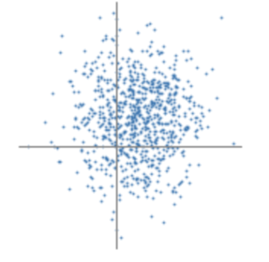
\includegraphics[width=0.4\textwidth]{chapters/chapter 10/covariance 3.png}}
\end{floatrow}
\end{figure}

Սա նշանակում է, որ $\Cov[X, Y]$-ը ցույց է տալիս $X$-ի ու $Y$-ի միջև եղած \textit{գծային կախումը՝} թե միջինում մեկի գծային աճը որքան փոփոխության է հանգեցնում մյուսի արժեքում (և հակառակը)։ Ստացված թիվը համաչափ է՝
\[
\Cov[X, Y] = \Cov[Y, X]
\]

\begin{example}
Նետենք $3$ մետաղադրամ, $X$-ով նշանակենք գիր ընկածների թիվը, $Y$-ով՝ ղուշ ընկածներինը։ Փորձենք հաշվել $\Cov[X, Y]$-ը։

Նախ, ի՞նչ հնարավոր արժեքներ կարող են ընդունել $X$-ն ու $Y$-ը միաժամանակ՝
\begin{itemize}
    \item $X=0$, $Y=3$
    \item կամ $X=1$, $Y=2$
    \item կամ $X=2$, $Y=1$
    \item կամ էլ $X=3$, $Y=0$
\end{itemize}
Որքա՞ն է, ասենք, $X=1$ և $Y=2$ լինելու հավանականությունը․\marginnote{արդյո՞ք $X$-ն ու $Y$-ն անկախ են}
\[
\PP[(X = 1) \text{ և } (Y = 2)] =\ ?
\]
Կարող ենք այս պատահույթը բաժանել երեք ենթադեպքի՝
\begin{itemize}
    \item առաջինը գիր, մյուս երկուսը ղուշ՝ ԳՂՂ
    \item երկրորդը գիր, մյուս երկուսը ղուշ՝ ՂԳՂ
    \item երրորդը գիր, մյուս երկուսը ղուշ՝ ՂՂԳ
\end{itemize}
Սրանցից յուրաքանչյուրի հավանականությունը
\[
\PP[\text{ԳՂՂ}] = 
\PP[\text{ՂԳՂ}] = 
\PP[\text{ՂՂԳ}] = 
\frac{1}{2} \cdot \frac{1}{2} \cdot \frac{1}{2} = \frac{1}{8}
\]
է, հետևաբար
\[
\PP[(X = 1) \text{ և } (Y = 2)] = 3 \cdot \frac{1}{8} = \frac{3}{8}
\]
և ճիշտ նույն ձևով\marginnote{վերևում գրվածի մեջ փոխենք «գիր» և «ղուշ» բառերի տեղերը} $\PP[(X = 2) \text{ և } (Y = 1)] = \dfrac{3}{8}$։

\newpage

Նման եղանակով հաշվելով մյուս երկու դեպքերի հավանականություն\-ները՝ կունենանք այսպիսի պատկեր․
\begin{center}
  \begin{tabular}{|c|c|c|}
    \hline
    $X$ & $Y$ & \textbf{հավանականություն} \\
    \hline
    $0$ & $3$ & $1/8$ \\
    \hline
    $1$ & $2$ & $3/8$ \\
    \hline
    $2$ & $1$ & $3/8$ \\
    \hline
    $3$ & $0$ & $1/8$ \\
    \hline
  \end{tabular}
\end{center}
Այժմ հաշվենք $X$-ի ու $Y$-ի մաթսպասումները՝
\[
\E[X] = 
0 \cdot \frac{1}{8} +
1 \cdot \frac{3}{8} +
2 \cdot \frac{3}{8} +
3 \cdot \frac{1}{8} =
1.5 = \E[Y]
\]
և հանենք դրանք յուրաքանչյուր տողում գրված արժեքներից․
\begin{center}
  \begin{tabular}{|c|c|c|}
    \hline
    $X - \E[X]$ & $Y - \E[Y]$ & \textbf{հավանականություն} \\
    \hline
    $-1.5$ & $1.5$ & $1/8$ \\
    \hline
    $-0.5$ & $0.5$ & $3/8$ \\
    \hline
    $0.5$ & $-0.5$ & $3/8$ \\
    \hline
    $1.5$ & $-1.5$ & $1/8$ \\
    \hline
  \end{tabular}
\end{center}
Կունենանք, որ 
\begin{align*}
\PP\big[(X - \E[X])(Y - \E[Y]) = -2.25\big] &= \frac{2}{8}\\
\PP\big[(X - \E[X])(Y - \E[Y]) = -0.25\big] &= \frac{6}{8}
\end{align*}
հետևաբար $X$-ի ու $Y$-ի կովարիացիան կլինի 
\[
\E\left[(X - \E[X])(Y - \E[Y])\right]
= -2.25 \cdot \frac{2}{8} + (-0.25) \cdot \frac{6}{8}
= -\frac{3}{4} = -0.75
\]
Ստացվեց բացասական կովարիացիա․ իրոք, ըստ սահմանման՝ երբ $X$-ը աճում է, $Y$-ը պիտի նվազի։
\end{example}

\question{Իսկ որքա՞ն է $\Cov[X, X+Y]$-ը (առանց հաշվելու)։}

Ինչպես կարող եք ենթադրել, եթե երկու պատահական մեծություններ իրարից անկախ են, նրանց կովարիացիան $0$ է՝\marginnote[*+2]{$X-\E[X]$-ն ու $Y-\E[Y]$-ն անկախ են}
\begin{align*}
\Cov[X, Y] &= \E\left[(X - \E[X])(Y - \E[Y])\right]
\\&= \E\left[X - \E[X]\right] \cdot \E\left[Y - \E[Y]\right]
= (\E[X] - \E[X]) \cdot (\E[Y] - \E[Y]) = 0
\end{align*}
բայց հակառակը ոչ միշտ է ճիշտ։ Թեկուզ միայն այն պատճառով, որ

\warning{Կովարիացիան ցույց է տալիս միայն պատահական մեծությունների միջև եղած \textbf{գծային} կապը։}

Այսինքն՝ հնարավոր է, որ պատահական մեծությունները իրար հետ կապված լինեն (ոչ թե գծային, այլ ասենք՝ քառակուսային կապով), բայց կովարիացիան դա չկարողանա «տեսնել»։

\newpage

\begin{example}
Ենթադրենք $X$ պատահական մեծությունն ընդունում է երեք արժեք՝
\[
\PP[X = -1] = \PP[X = 0] = \PP[X = 1] = \frac{1}{3}
\]
իսկ $Y$-ը նրա քառակուսին է՝ $Y = X^2$։ \marginnote{կարո՞ղ եք ինքնուրույն շարունակել} Բնականաբար $X$-ն ու $Y$-ն անկախ չեն, սակայն
\[
\E[X] = 0, \qquad \E[Y] = \frac{2}{3}
\]

\begin{marginfigure}
    \centering
    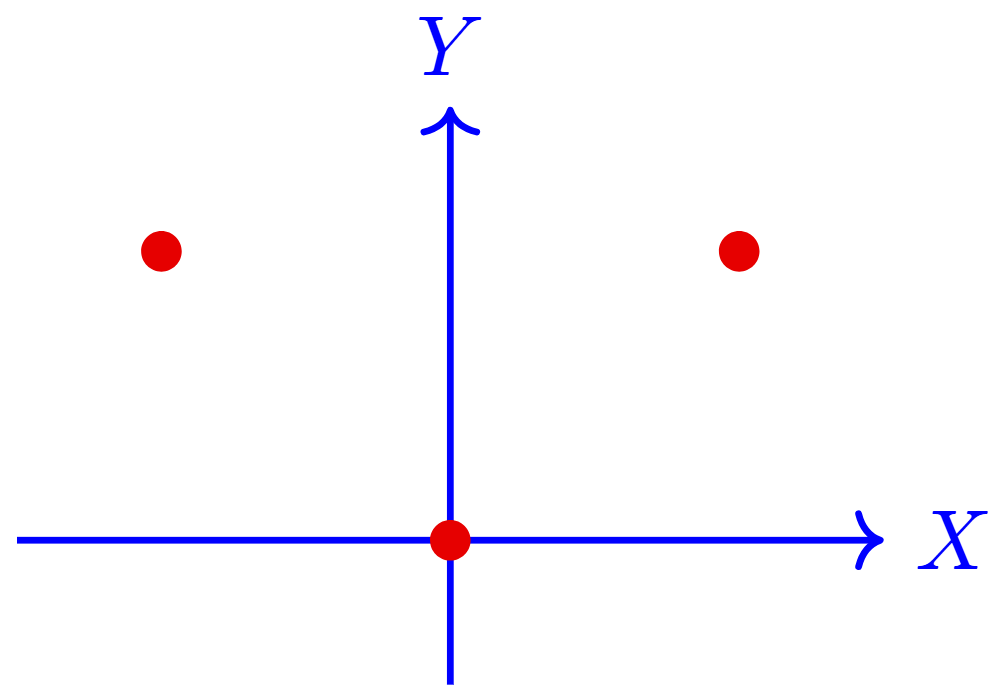
\includegraphics[width=0.8\linewidth]{chapters/chapter 10/three points.png}
\end{marginfigure}

% \begin{tikzpicture}[scale=1.2]
%   \draw[->, thick, blue] (-1.5,0) -- (1.5,0) node[anchor=west] {\textcolor{blue}{$X$}};
%   \draw[->, thick, blue] (0,-0.5) -- (0,1.5) node[anchor=south] {\textcolor{blue}{$Y$}};
%   \fill[myred] (-1,1) circle (2pt);
%   \fill[myred] (0,0) circle (2pt);
%   \fill[myred] (1,1) circle (2pt);
% \end{tikzpicture}

և հնարավոր արժեքների հավանականություններն են․
\begin{center}
  \begin{tabular}{|c|c|c|}
    \hline
    $X$ & $Y$ & \textbf{հավանականություն} \\
    \hline
    $-1$ & $1$ & $1/3$ \\
    \hline
    $0$ & $0$ & $1/3$ \\
    \hline
    $1$ & $-1$ & $1/3$ \\
    \hline
  \end{tabular}
\end{center}
որտեղից ստանում ենք՝
\[
\Cov[X, Y] = 
(-1) \cdot \frac{2}{3} \cdot \frac{1}{3} +
0 \cdot 0 \cdot \frac{1}{3} +
1 \cdot \frac{2}{3} \cdot \frac{1}{3} = 0
\]
Իրոք, թեև $X$-ն ու $Y$-ն անկախ չեն, բայց $X$-ի և՛ մեծանալիս, և՛ փոքրանալիս $Y$-ը փոխվում է նույն ձև՝ մեծանում է, այսինքն դրանց միջև եղած կապը գծային չէ՝ $\Cov[X, Y] = 0$:
\end{example}

Այնուամենայնիվ, կովարիացիան շատ օգտակար գործիք է երկու մեծությունների հնարավոր կապը բացահայտելու համար։ Վերևում արված երկար ու ձանձրալի հաշվարկներից խուսափելու համար կովարիացիայի սահմանման մեջ բացենք փակագծերն ու պարզեցնենք․ կստանանք՝
\[
\Cov[X, Y] = \E[XY] - \E[X] \cdot \E[Y]
\]
որտեղից կունենանք մեզ հետաքրքրող մյուս հատկությունները՝
\begin{align*}
\Cov[c \cdot X, Y] &= \Cov[X, c \cdot Y] = c \cdot \Cov[X, Y] \\
\Cov[X, Y_1 + Y_2] &= \Cov[X, Y_1] + \Cov[X, Y_2]
\end{align*}
իսկ մասնավորապես դրանցից երկրորդի շնորհիվ՝ ոչ այնքան հետաքրքիր հաջորդ հատկությունը․
\begin{align*}
\Cov[X_1 + X_2, Y_1 + Y_2]&= \Cov[X_1, Y_1] + \Cov[X_1, Y_2] \\&+ \Cov[X_2, Y_1] + \Cov[X_2, Y_2]
\end{align*}
որը կասկածելիորեն նման է բազմապատկելիս փակագծերը բացելուն՝ $(a+b)(c+d) = \dots$: 

\question{Ի՞նչ կստացվի, եթե $Y$-ի փոխարեն տեղադրենք $X$։ Ինչպե՞ս կմեկնաբանեք ստացվածը։}

Բնականաբար, եթե պատահական մեծություններից մեկը \marginnote[*+1]{$=$ ընդունում է միայն մեկ արժեք} հաստատուն է՝ $Y=c$, ապա $\Cov[X, Y] = 0$։


\section{Կոռելացիա}

\textit{— Բայց մի րոպե,— կարող եք հարցնել,— ի՞նչ է նշանակում $\Cov[X, Y] = 60$․ վերջը կա՞ գծային կապ, թե՞ ոչ։}

Իհարկե, եթե կովարիացիան դրական է, նշանակում է՝ որոշակի կապ կա, բայց ինչպե՞ս հասկանալ՝ այդ կապը մե՞ծ է, թե՞ փոքր, այսինքն՝ $X$-ն ու $Y$-ը մաքուր մեկը մյուսից գծային կապված մեծություննե՞ր են, թե՞ պարզապես շատ աղոտ կերպով կապված ինչ-որ բաներ։ 

\warning{$\Cov[X, Y]$-ի՝ մոդուլով մեծ կամ փոքր լինելը ինքնին շատ բան չի նշանակում։}

Չէ՞ որ եթե ասենք՝ $Y$-ը բազմապատկենք $1000$-ով,\marginnote{եթե $Y$-ը մարդու հասակն է մետրով, ${1000\cdot Y}$-ը կլինի նույն հասակը մմ-ով} դրանից $X$-ի ու $Y$-ի միջև եղած գծային կապը պետք է որ չփոխվի, բայց այ կովարիացիան միանգամից կմեծանա։ Ուրեմն որպեսզի ունենանք պատահական մեծությունների գծային կապը ցույց տվող մի բացարձակ թիվ՝ բոլորի համար ընդհանուր մասշտաբով, պետք է $\Cov[X, Y]$-ը բաժանենք այնպիսի բանի վրա, որ ստացվածը լինի ինչ-որ ֆիքսված միջակայքում։

\question{Ինչի՞ վրա էինք բաժանում $\va \cdot \vb$-ն, որպեսզի ստանայինք $\va$-ի ու $\vb$-ի կազմած անկյունը/դրա կոսինուսը։}

\begin{definition}
$X$ և $Y$ պատահական մեծությունների \textbf{կոռե\-լա\-ցիա}\marginnote{կամ \textit{Փիրսընի կոռելացիայի գոր\-ծա\-կից}} կանվանենք հետևյալ թիվը՝
\[
\rho_{X, Y} = \frac{\Cov[X, Y]}{\sqrt{\Var[X] \cdot \Var[Y]}}
\]
\end{definition}

Այս թիվն արդեն կգտնվի $[-1, 1]$ միջակայքում և կլինի երկու մեծություն\-ների գծային կապը ցույց տվող \textit{ունիվերսալ} գործիք․
\begin{theorem}
\[
-1 \le \rho_{X, Y} \le 1
\]
և հավասար է $\pm 1$-ի միմիայն այն դեպքում, երբ $Y = kX + b$:
\end{theorem}

Կրկին, կարդալուց լավ է \href{https://www.geogebra.org/m/w5q22bzu}{աչքով տեսնել և բզբզալ}։

\begin{figure}[b]
    \centering
    \caption*{կոռելացիան $X$-ի ու $Y$-ի որոշ արժեք\-նե\-րի դեպքում}
    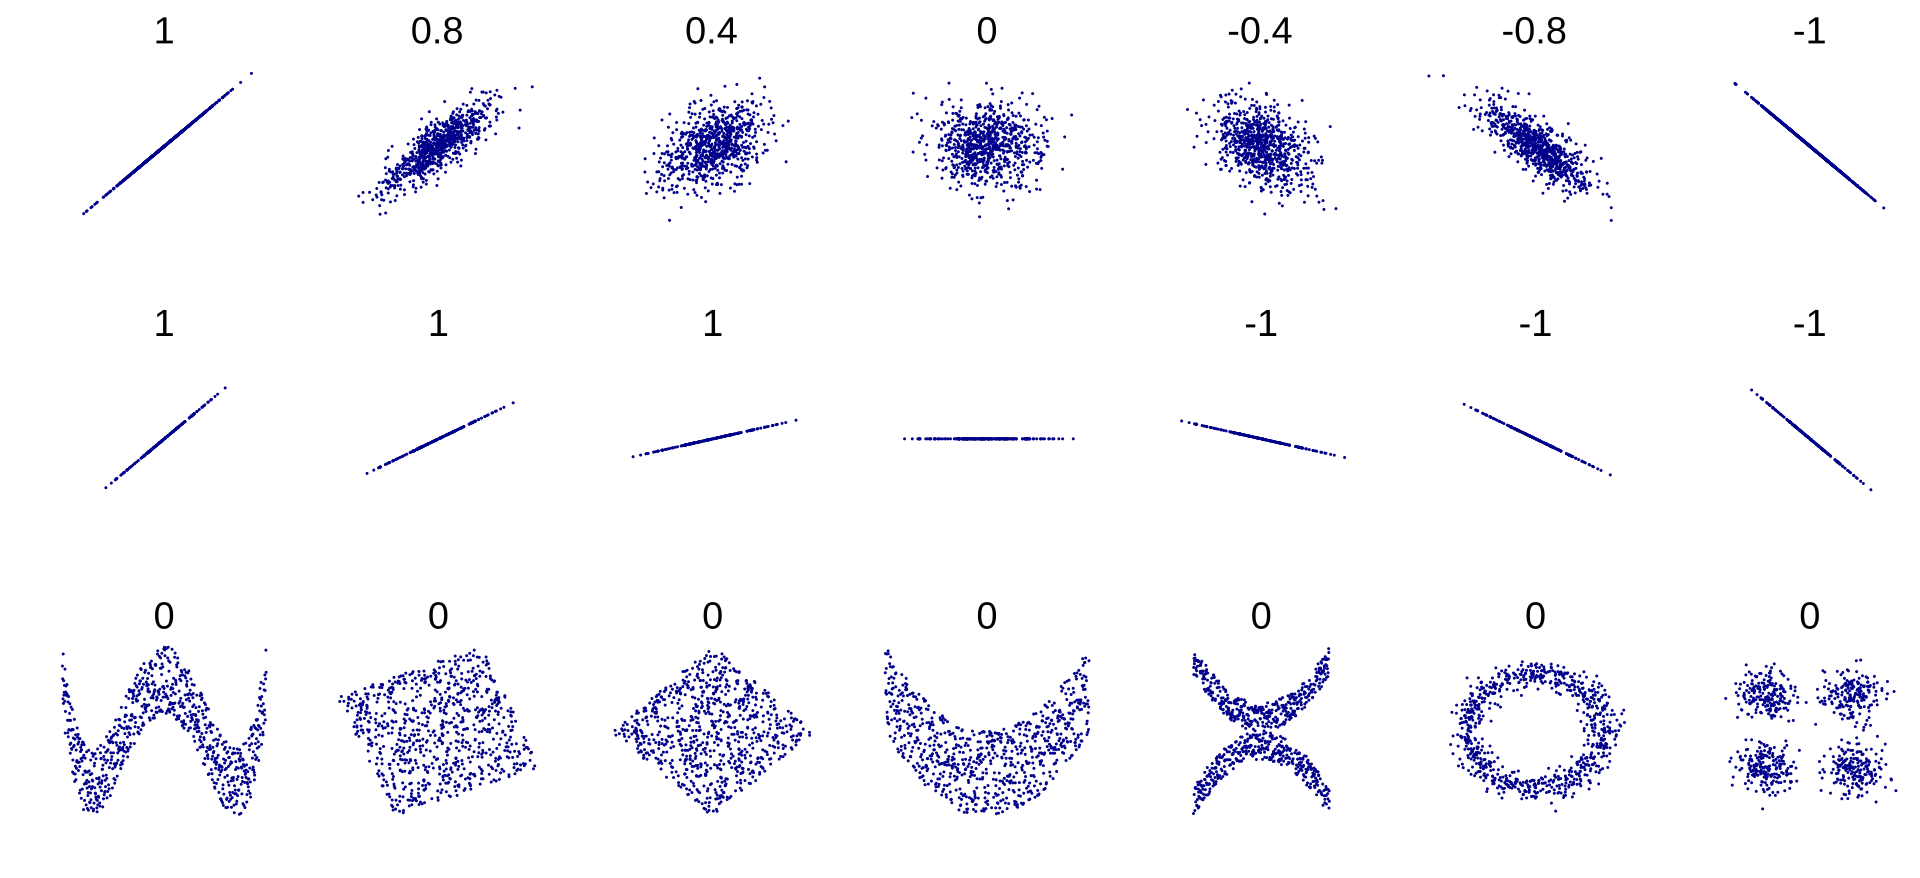
\includegraphics[width=0.9\linewidth]{chapters/chapter 10/correlation.png}
\end{figure}


\section{Բաշխումներ}

Եթե որոնեք, թե ինչպես են բաշխված այս կամ այն երկրում մարդկանց աշխատավարձերը, հասակները, քաշերը և այլն, կնկատեք մի տար\-օրի\-նակ նմանություն դրանց \href{https://images.app.goo.gl/viKPLRbQKCsQfbhLA}{խտության գրաֆիկներում}․ կարծես բոլորը մո\-տա\-վո\-րա\-պես նույն գրաֆիկը լինեն՝ ինչ-որ չափով ձգված, սեղմված կամ տեղա\-շարժ\-ված։ Առանց պատ\-ճառ\-նե\-րի մեջ խորանալու նկատենք, որ այսպիսի նմա\-նու\-թյուն\-ներ հանդիպում են ամե\-նա\-տար\-բեր պրոցեսների արդյունքում առա\-ջա\-ցող պատա\-հա\-կան մեծու\-թյուն\-ների բաշխումներում։ Ուրեմն եթե 
% այդ տարբեր, բայց միմյանց նման բաշխումներին տանք մեկ միասնական անուն ու 
ընդհանուր դեպքում այդ պատահական մեծություններից մեկի բաշխումը հետազոտենք, ապա հետազոտած կլինենք նաև նույն կաղապարով/ֆորմայով ստացված մյուս բաշխումները։

Իրականում մենք մի անգամ նման բան արել ենք, երբ
\begin{itemize}
\item $[0, 10]$ հատվածում ընտրում ենք պատահական կետ
\item $12$:$00$-$13$:$00$ պատահական պահի գալիս ենք կանգառ
\item գեներացնում ենք պատահական թիվ $(-1, 1)$ միջակայքում
\item $\dots$
\end{itemize}
այս բոլոր պատահական մեծություններին տվեցինք մեկ ընդհանրական անուն՝\marginnote{իհարկե համարելով, որ ցանկացած տե\-ղա\-մասում գտնվող արժեքներն ունեն նույն հավանականությունը} ասելով, որ դրանք \textit{հավասարաչափ բաշխում} ունեն, և գտնելով $\operatorname{U}(a, b)$ բաշխումով ցանկացած պատահական մեծության {\rm CDF}-ն ու {\rm PDF}-ը (որոնք ազատ կարող ենք օգտագործել նշված բոլոր մասնավոր օրինակների համար)։  

Եկեք այժմ նույն կերպ դիտարկենք մի քանի հիմնական բաշխումներ (անգիր անել պետք չէ), որոնք հանդիպում են տարբեր պրոցեսներում։ Սկսենք դիսկրետ բաշխումներից։

\begin{description}
\item[Բեռնուլիի բաշխում․] 
Դիտարկենք հետևյալ իրավիճակները՝
\begin{itemize}
    \item նետում ենք մետաղադրամ
    \item մտնում ենք վարորդական իրավունքի քննության
    \item կրակում ենք թիրախին
    \item ջնջում ենք լոտո
\end{itemize}
Դրանցից յուրաքանչյուրում կա երկու հնարավոր տարբերակ՝ գիր կամ ղուշ, անցնել կամ կտրվել, դիպչել կամ ոչ, շահել կամ չշահել, և այլն։ Այսպիսի փորձերը կանվանենք \textit{Բեռնուլիի փորձեր,} իսկ երկու հնարավոր արժեք ընդունող (մեկը՝ $p$, մյուսը՝ $1-p$ հավանականությամբ) ցանկացած պատահական մեծության մասին կասենք, որ այն ունի Բեռնուլիի բաշխում՝
\[
X \sim \operatorname{Bernoulli}(p)
\]
Հեշտությամբ կարող ենք հաշվել, որ այս դեպքում
\[
\E[X] = p, \qquad \Var[X] = p(1-p)
\]

\item[Երկրաչափական բաշխում․]
Իսկ ի՞նչ, եթե որոշենք լոտոներ ջնջել այնքան, մինչև վերջապես շահենք (կամ ավելի խելացի միտք՝ քննություն տանք այնքան, մինչև վերջապես անցնենք)։ Քանի՞ անգամ կպահանջվի մինչև առաջին անգամ շահելը/անցնելը, կամ որ նույնն է՝ քանի՞ անգամ պետք է կրկնենք շահելու $p$ հավանականություն ունեցող Բեռնուլիի փորձը, մինչև առաջին անգամ շահենք։

Նշանակենք այդ փորձերի քանակը $X$-ով և գտնենք $p_X(k)$-ն։ Նախ՝ հավանականությունը, որ $X=1$, այսինքն՝ որ հենց առաջին փորձից կստացվի անցնել քննությունը, $p$ է։ 

Իսկ որ $X=2$, այսինքն՝ առաջին անգամը կկտրվենք, իսկ երկ\-րորդին արդեն կանցնենք, հավասար է
\[
\PP[X = 2] = \underbrace{\color{myred}(1 - p)}_{\substack{\text{$1$-ինը}\\\text{կտրվենք}}} \ \cdot \underbrace{\color{mygreen}p}_{\substack{\text{$2$-րդը}\\\text{անցնենք}}}
\]
Հավանականությունը, որ $X=3$՝
\[
\PP[X = 3] = \underbrace{\color{myred}(1 - p)}_{\substack{\text{$1$-ինը}\\\text{կտրվենք}}} \ \cdot \ \underbrace{\color{myred}(1 - p)}_{\substack{\text{$2$-րդը}\\\text{կտրվենք}}} \ \cdot \underbrace{\color{mygreen}p}_{\substack{\text{$3$-րդը}\\\text{անցնենք}}}
\]

\begin{marginfigure}
    \centering
    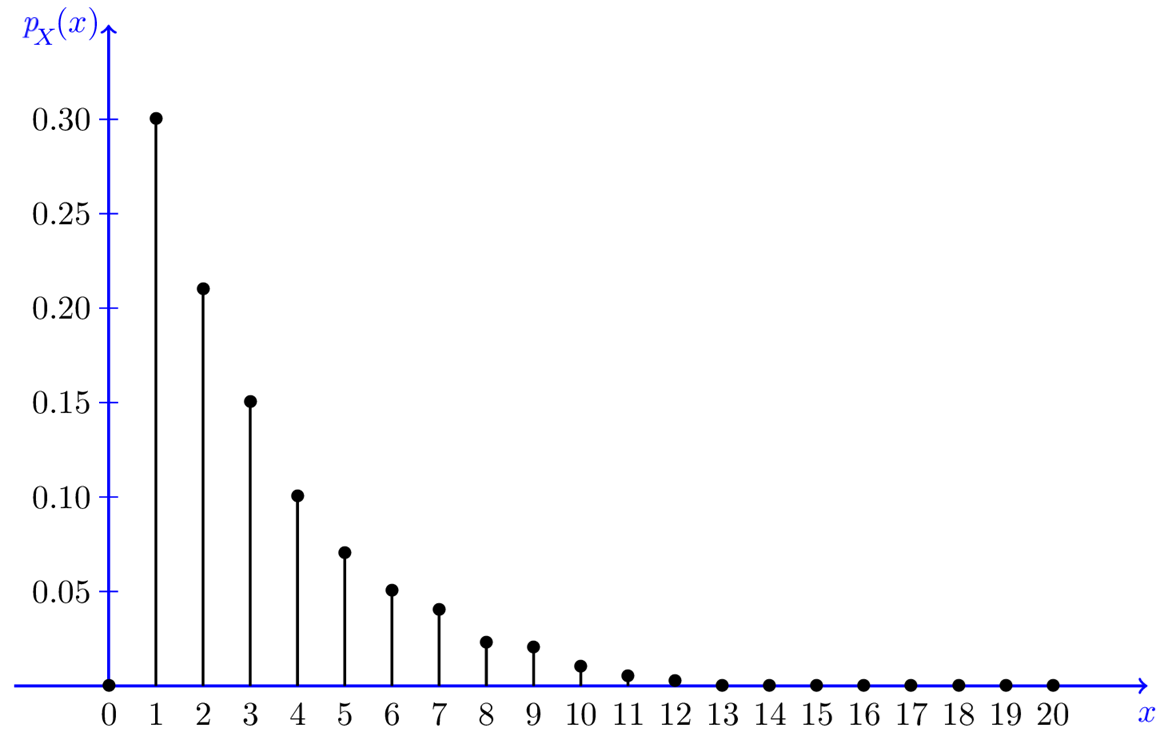
\includegraphics[width=\linewidth]{chapters/chapter 10/geometric.png}
    \caption*{$X$-ի {\rm PMF}-ը, երբ $p=0.3$}
\end{marginfigure}

Եվ այդպես շարունակ՝
\[
\PP[X = k] = {\color{myred}(1 - p)} \cdot {\color{myred}(1 - p)} \cdot \ldots \cdot {\color{myred}(1 - p)} \cdot {\color{mygreen}p} 
= (1 - p)^{k-1} \cdot p
\]
այսինքն $k$-ն $1$-ով մեծացնելիս հավանականությունը բազմա\-պատկ\-վում է $(1-p)$-ով՝ դառնալով երկրաչափական պրոգրեսիա։ Նման դեպքերում կասենք, որ $X$-ն ունի երկրաչափական բաշխում՝
\[
X \sim \operatorname{G}(p)
\]
և կունենանք
\[
\E[X] = \frac{1}{p}, \qquad \Var[X] = \frac{1 - p}{p^2}
\]

\question{Կարո՞ղ եք ապացուցել, որ եթե արդեն իսկ $100$ անգամ \newline ջնջել ու չեք շահել, դա Ձեզ ավելի մոտ չի դարձնում շահելուն։}
Այլ կերպ ասած՝
\[
\PP[X > m + n \mid X > m] = \PP[X > n]
\]
Այս հատկության մասին ասում են, որ երկրաչափական բաշխումը \textit{հիշողություն չունի։}

\item[Բինոմական բաշխում․]
Մյուս կողմից՝ եթե իրար հետևից հանձնեք մի քանի քննություն, ասենք՝ $n$ հատ, և ամեն մեկում ունենաք անցնելու նույն $p$ հավանականությունը, կարող եք հարցնել՝ որքա՞ն է հավանական, որ կանցնեք բոլոր $n$ քննությունները, կամ քննությունների կեսը, կամ $3$ հատը, և այլն։

Եթե $X$-ով նշանակենք, թե այդ $n$ Բեռնուլիի փորձերից քանի՞սն են հաջողությամբ պսակվել, կունենանք՝\marginnote[*+4]{$C_n^k$-ն կարդացվում է «զուգորդություն $n$-ից $k$-ական», նշանակվում է նաև $\displaystyle \binom{n}{k}$}
\[
\PP[X = k] \ = \underbrace{C_n^k}_{\substack{\text{$n$ հատից $k$ հատ}\\\text{ընտրելու ձևերը}}} \cdot \ \overbrace{p^k}^{\substack{\text{$k$ անգամ}\\\text{կանցնենք}}} \cdot \ \underbrace{(1 - p)^{n-k}}_{\substack{\text{$n-k$ անգամ}\\\text{կկտրվենք}}}
\]
որտեղ $C_n^k = \dfrac{n!}{k!\cdot(n-k)!}$: 

\begin{marginfigure}
    \centering
    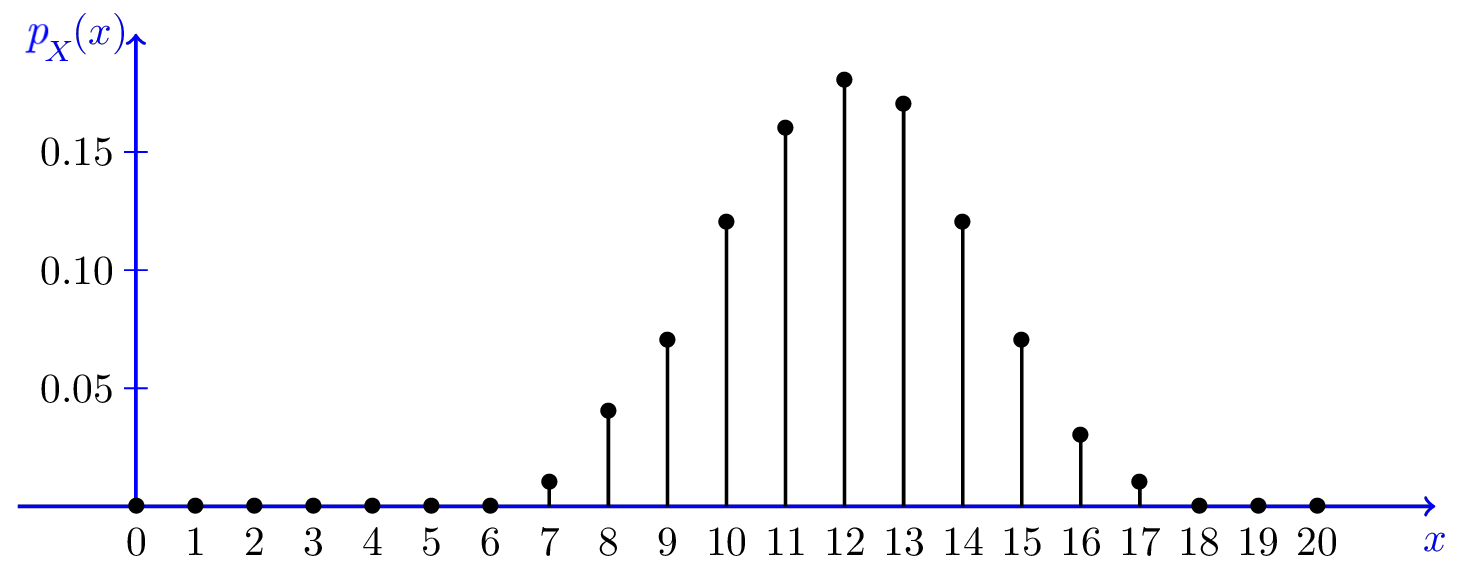
\includegraphics[width=\linewidth]{chapters/chapter 10/binomial.png}
    \caption*{$X$-ի {\rm PMF}-ը, երբ $n=20$, $p=0.6$}
\end{marginfigure}

Այս բանաձևերը պետք չէ անգիր անել․ դրանց շատ գեղեցիկ բացատրությունն ու դուրս բերումը կարող եք գտնել \href{https://www.youtu.be/8idr1WZ1A7Q}{այստեղ} կամ \href{https://www.youtu.be/6YzrVUVO9M0}{այստեղ}։ Այս դեպքում կասենք, որ $X$-ն ունի բինոմական բաշխում՝
\[
X \sim \operatorname{B}(n, p)
\]
և կունենանք՝
\[
\E[X] = np, \qquad \Var[X] = np(1-p) 
\]

\item[Պուասոնի բաշխում․] 
Եկեք ոչ թե իրար հետևից ինչ-որ փորձեր կրկնենք, այլ պարզապես հաշվենք, թե
\begin{itemize}
    \item քանի հաճախորդ մտավ $13$:$00$-$14$:$00$ հատվածում
    \item քանի ավտովթար եղավ օրվա ընթացքում
    \item քանի զանգ եկավ սխալ համարից
    \item քանի գոլ եղավ խաղի ժամանակ
    \item քանի ավտոբուս անցավ կանգառով $1$ ժամում 
\end{itemize}
այսինքն՝ հաշվենք, թե ամեն անգամը նախորդից անկախ տեղի ունեցող մի որևէ երևույթից քանի անգամ արձանագրվեց ֆիքսված ժամանակամիջոցում։ Ստացված քանակը (ենթադրենք՝ խանութ մտած այցելուների) նշանակենք $X$-ով։

Եթե ասենք՝ նախորդ շաբաթվա տվյալների հիման վրա իմանանք, թե միջինում\marginnote{այսինքն՝ վայրկյանը մեկ նա\-յում ենք՝ մարդ մտա՞վ, թե՞ ոչ․ \[X \sim \operatorname{B}\left(3600, \dfrac{\lambda}{3600}\right)\] իսկ սրա {\rm PMF}-ը  $\approx \dfrac{\lambda^k}{k!} \cdot e^{-\lambda}$ է} $13$:$00$-ից $14$:$00$-ը քանի հոգի է մտնում խանութ (օրինակ՝ միջինում $\lambda=20$ հոգի), ապա կունենանք՝
\[
\PP[X = k] = \frac{\lambda^k}{k!} \cdot e^{-\lambda}
\]
և կասենք, որ $X$-ն ունի Պուասոնի բաշխում՝
\[
X \sim \operatorname{Poisson}(\lambda)
\]
\begin{marginfigure}
    \centering
    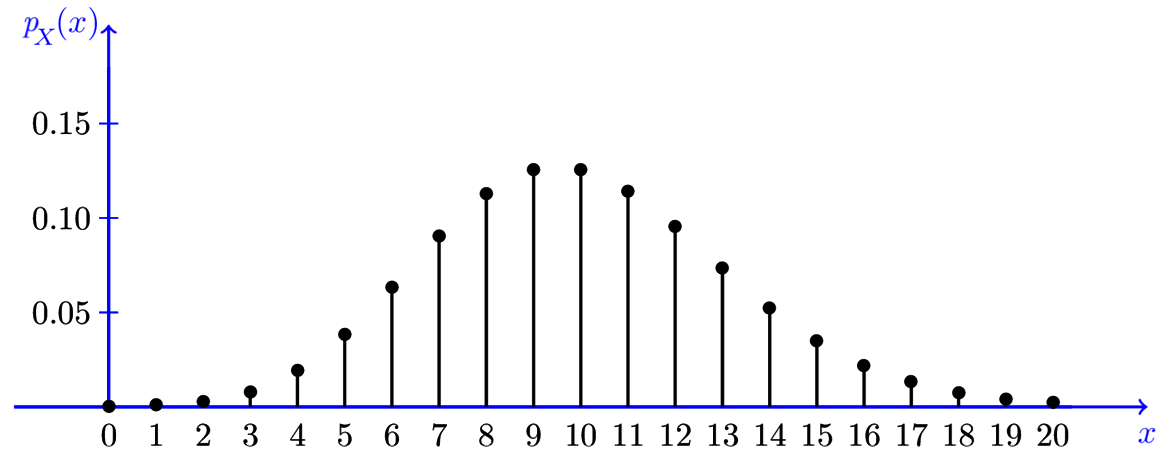
\includegraphics[width=\linewidth]{chapters/chapter 10/poisson.png}
    \caption*{$X$-ի {\rm PMF}-ը, երբ $\lambda=10$}
\end{marginfigure}
\question{Ճանաչո՞ւմ եք այս թվերը։}

Այս դեպքում մաթսպասումն ու վարիացիան համընկնում են՝
\[
\E[X] = \lambda, \qquad \Var[X] = \lambda
\]
\end{description}

Եվ այդպես շարունակ։ Կան \href{https://en.wikipedia.org/wiki/List_of_probability_distributions}{բազմաթիվ} այլ օգտակար բաշխումներ, որոնք հանդիպում են տարբեր իրավիճակներում, բայց դրանք անգիր հիշելու կամ բոլորը իմանալու կարիք չկա։

Անցնենք անընդհատ բաշխումներին։

\begin{description}
\item[Հավասարաչափ բաշխում․]
Անձամբ ճանաչում ենք։ Ավելացնենք միայն, որ եթե $X \sim \operatorname{U}(a, b)$, ապա
\[
\E[X] = \frac{a + b}{2}, \qquad \Var[X] = \frac{(b - a)^2}{12}
\]

\item[Ցուցչային {\normalfont (էքսպոնենցիալ)} բաշխում․]
Սա մեր երկրաչափական բաշխ\-ման անընդհատ անալոգն է։ Պատկերացրեք՝ հենց նոր ան\-ցավ ավտոբուսը, և կանգնած սպասում եք, թե քանի րոպեից կգա հաջորդը։ Այդ $X$ ժամանակահատվածը, \marginnote{կարող ենք համարել, որ աչքերը բացում ենք, նայում՝ ավտոբուս կա, թե ոչ, փա\-կում, \href{https://youtu.be/TZTjr-DN9xY?si=vfGqcFPmMgqd-bqp&t=1794}{ապա նորից}, այնքան մինչև գա} այսինքն՝ թե որքան է պետք սպասել, մինչև ինչ-որ երևույթ նորից տեղի ունենա, ունի ցուցչային բաշխում՝
\[
X \sim \operatorname{Exp}(\lambda)
\]
որտեղ $\lambda$-ով նշանակում ենք, թե միջինում որքան ժամանակը մեկ է գալիս ավտոբուսը։

\begin{marginfigure}
    \centering
    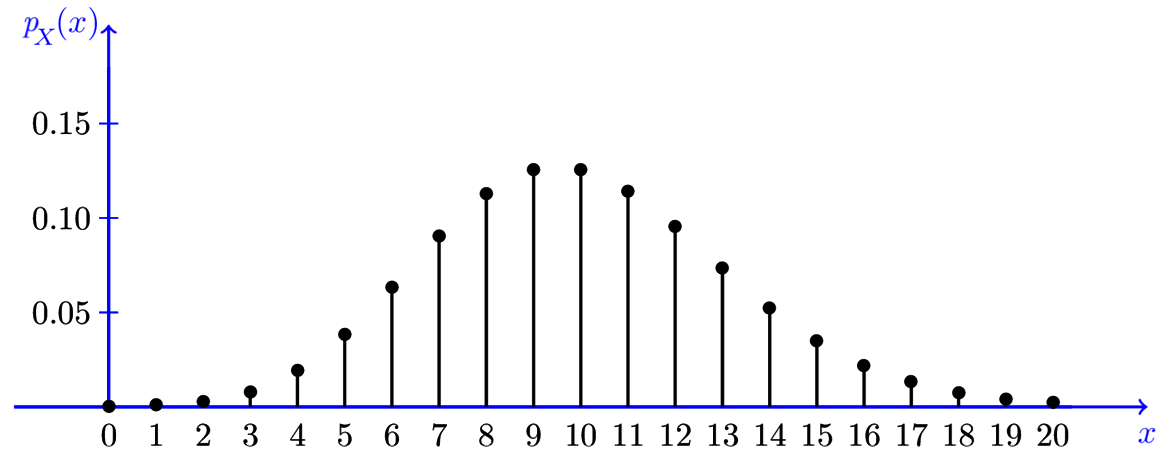
\includegraphics[width=\linewidth]{chapters/chapter 10/poisson.png}
    \caption*{$X$-ի {\rm PDF}-ը տարբեր $\lambda$-ների դեպքում}
\end{marginfigure}

$X$-ի խտության ֆունկցիան կունենա հետևյալ տեսքը՝
\[
f_X(x) = \begin{cases}
    \lambda e^{-\lambda x} & \text{եթե } x \ge 0 \\
    0 & \text{եթե } x < 0
\end{cases}
\]
իսկ մաթսպասումն ու վարիացիան կլինեն
\[
\E[X] = \frac{1}{\lambda}, \qquad \Var[X] = \frac{1}{\lambda^2}
\]
Ինչպես երկրաչափական, այնպես էլ ցուցչային բաշխումը հիշո\-ղու\-թյուն չունի՝
\[
\PP[X > a + b \mid X > b] = \PP[X > a]
\]
այսինքն՝ եթե արդեն իսկ $b$ րոպե սպասել ենք, բայց ավտոբուսը դեռ չի եկել, ապա հավանականությունը, որ այն կգա ևս $a$ րոպե անց, նույնն է, ինչ եթե սկզբի $b$ րոպեն սպասած չլինեինք։ Ավտոբուսը չգիտի՝ իրեն սպասել ենք, թե ոչ․ մեր սպասելուց ոչինչ չի փոխվում։

\item[Նորմալ {\normalfont (գաուսյան)} բաշխում․]
Ինչ-որ իմաստով՝ սա ամենակարևոր բաշխումն է։ Պատկերացրեք՝ եթե
\begin{itemize}
    \item նետենք $100$ հատ զառ
    \item չափենք պատահական $1000$ հոգու հասակ
    \item հաշվենք $500$ պատահական բառերի տառեր
    \item իրար վրա լցնենք \href{https://youtu.be/UCmPmkHqHXk}{տարերային շարժվող գնդիկներ}
\end{itemize}
ու նայենք, թե ինչ $X$ թիվ ենք ստանում \marginnote{այսինքն՝ նույն բաշխումը ունեցող մեծ թվով պատահական մեծությունների միջինը} \textbf{միջինում,} ապա
այդ $X$-ը կլինի պատահական մեծություն (ընդ որում՝ անընդհատ), և նրա խտության ֆունկցիան կունենա հետևյալ տեսքը՝
\[
f_X(x) = \frac{1}{\sqrt{2\pi \sigma^2}}e^{-\dfrac{(x - \mu)^2}{2\sigma^2}}
\]

\begin{figure}[b]
    \centering
    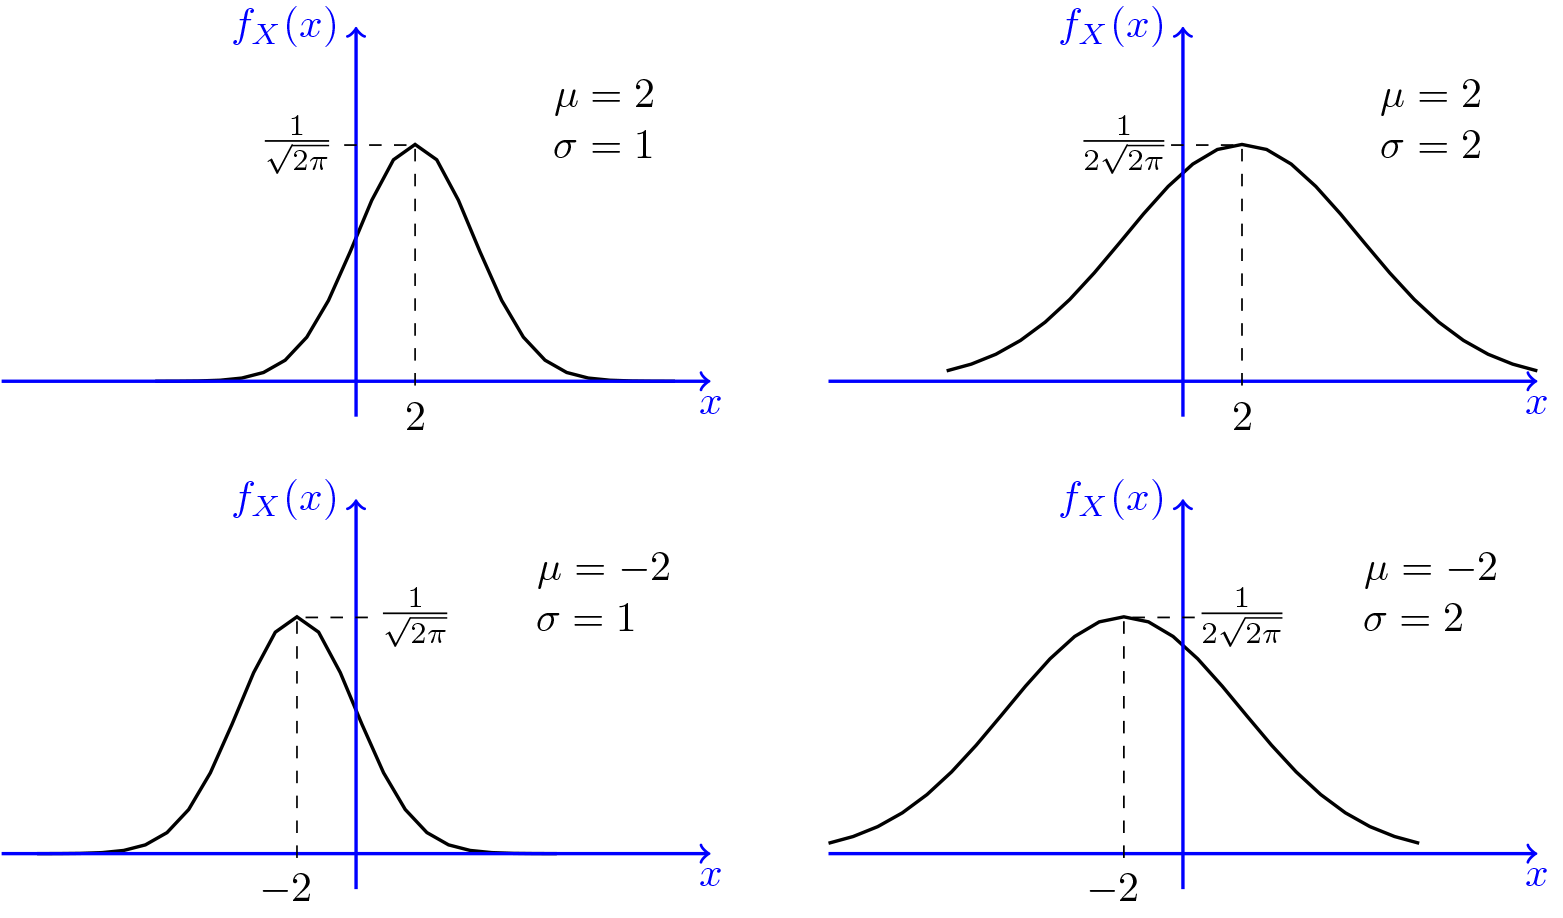
\includegraphics[width=0.85\linewidth]{chapters/chapter 10/normal.png}
\end{figure}

որտեղ $\mu$-ն ու $\sigma^2$-ն նրա մաթսպասումն ու վարիացիան են՝
\[
\E[X] = \mu, \qquad \Var[X] = \sigma^2
\]

\question{Ինչպե՞ս կփոխվի $f_X$-ի գրաֆիկը, եթե $\mu$-ն մեծացնենք \newline $7$-ով, իսկ $\sigma$-ն բազմապատկենք $2$-ով:}

Թե ինչու է սա ճիշտ, և ինչու է արդյունքում ստացվում այսպիսի զանգակաձև կոր, բխում է «կենտրոնական սահմանային թեորեմ» կոչվող մի հետաքրքիր փաստից, որը մենք կշրջանցենք և պարզապես կասենք, որ $X$-ն ունի նորմալ կամ գաուսյան բաշխում՝
\[
X \sim \operatorname{N}(\mu, \sigma^2)
\]
Մասնավորապես ${X \sim \operatorname{N}(0, 1)}$ դեպքում կասենք, որ $X$-ն ունի \textit{ստան\-դարտ} նորմալ բաշխում։ Նորմալ բաշխում ունեցող ցան\-կա\-ցած $X$-ից կարող ենք իր $\mu$ միջինը հանելով ու $\dfrac{1}{\sigma}$-ով բազ\-մա\-պատ\-կելով՝ այն դարձնել ստանդարտ նորմալ։
\end{description}


\bigskip 

\begin{theory}
.
\begin{itemize}
\item կարդալ [{\rm Blitzstein-Hwang}], 137-143, 156-159, 200, կամ [{\rm Grimmett-Welsh}], 30-32, 73-74 էջերը (մաթսպասում, վարիացիա)
\item տեսնել \href{https://www.countbayesie.com/blog/2015/2/20/random-variables-and-expectation}{մաթսպասումն} ու \href{https://www.countbayesie.com/blog/2015/2/21/variance-co-variance-and-correlation}{վարիացիան} կոնկրետ օրինակով 
\item կարդալ [{\rm Blitzstein-Hwang}], 300-304, կամ [{\rm Grimmett-Welsh}], 113-117 էջերը (կովարիացիա, կոռելացիա)
\item տեսնել, թե \href{https://dlsun.github.io/skis/discrete/named-distributions.html}{դիսկրետ} և \href{https://dlsun.github.io/skis/continuous/named-distributions.html}{անընդհատ} բաշխումներից որը երբ է հանդիպում
\item ըստ ցանկության՝ կարդալ բաշխումների մասին [{\rm Blitzstein-Hwang}], 100-103 (Բեռնուլի, բինոմական), 161-164 (Պուասոն), 201-202 (հավասարաչափ), 211-212 (նորմալ), 217-219 (ցուց\-չա\-յին) էջերը
\item ըստ ցանկության՝ դիտել կենտրոնական սահմանային թեո\-րեմի մասին \href{https://youtu.be/zeJD6dqJ5lo}{տեսանյութ} {\rm 3b1b}-ից
\end{itemize}
\end{theory}

\newpage

\section{Խնդիրներ}


\begin{problem}
Հնարամիտ ուստա Վարդանն առաջարկում է խաղալ հետևյալ խաղը։ Նետում եք զառը, և
\begin{itemize}
    \item եթե ընկնում է $1$, ուստա Վարդանը Ձեզ տալիս է $2\,500$ դրամ
    \item եթե ընկնում է $2$, տալիս է $5000$ դրամ
    \item եթե ընկնում է $3$, ոչ ոք ոչինչ չի տալիս
    \item եթե ընկնում է $4$ կամ $5$, Դուք եք $10\,000$ դրամ տալիս ուստա Վար\-դանին
    \item եթե ընկնում է $6$, տալիս եք $15\,000$ դրամ
\end{itemize}
Ցանկանո՞ւմ եք խաղալ այս խաղը։ Ինչո՞ւ։
\end{problem}


\begin{problem}
Վահեն զառի 
\includegraphics[height=1.6ex]{chapters/chapter 8/dice/4.png} կողմի վրա նկարեց ևս մի կետ՝ դարձնելով այն 
\includegraphics[height=1.6ex]{chapters/chapter 8/dice/5.png}, իսկ 
\includegraphics[height=1.6ex]{chapters/chapter 8/dice/1.png} կողմի վրա ավելացրեց երկու կետ՝ դարձնելով այն 
\includegraphics[height=1.6ex]{chapters/chapter 8/dice/3.png}։ 

Որքա՞ն է հավանականությունը, որ զառը նետելիս կընկնի $4$-ից մեծ թիվ։ Որքա՞ն են զառի մաթսպասումն ու վարիացիան։
\end{problem}


\begin{problem}
$52$ հատ խաղաթղթերից պատահականորեն քաշում եք մեկը։ Եթե
\begin{itemize}
    \item հանեցիք սիրտ, շահում եք $10\,000$ դրամ
    \item սիրտ չէ, բայց վրան մարդ է պատկերված, շահում եք $8\,000$ դրամ
    \item մնացած դեպքերում կորցնում եք $6\,000$ դրամ
\end{itemize}

Ձեռնտո՞ւ է խաղալ այս խաղը։ Միջինում որքա՞ն կշահեք/կկորցնեք ամեն խաղի արդյունքում։
\end{problem}


\begin{problem}
$X$ պատահական մեծության խտության ֆունկցիան է՝
\[
f_X(x) = \begin{cases}
    \frac{3}{x^4} & \text{եթե } x \ge 1 \\
    0 & \text{մնացած դեպքերում}
\end{cases}
\]
Գտեք $\E[X]$-ն ու $\Var[X]$-ը։
\end{problem}


\begin{problem}
$X$ պատահական մեծության խտության ֆունկցիան է՝
\[
f_X(x) = \begin{cases}
   2x & \text{եթե } 0 \le x \le 1 \\
   0 & \text{մնացած դեպքերում} 
\end{cases}
\]
Որքա՞ն են հետևյալ պատահական մեծություններից յուրաքանչյուրի մաթսպասումն ու վարիացիան․
\begin{enumerate}[label={\alph*}․]
\item $X$
\item $2X$
\item $2X + 7$
\item $(2X + 7)\cdot Y$
\end{enumerate}
որտեղ $Y$-ը պատահական նետված զառի թիվն է։
\end{problem}


\begin{problem}
$X$-ն ու $Y$-ը հավասարաչափ բաշխված անկախ պա\-տա\-հա\-կան մեծություններ են, ընդ որում՝
\[
X \sim \operatorname{U}(0, 2), 
\qquad
Y \sim \operatorname{U}(4, 10)
\]

\newpage

Կարո՞ղ եք գտնել
\begin{enumerate}[label={\alph*}․]
\item $X + Y$-ի մաթսպասումը
\item $XY$-ի մաթսպասումը
\item $X + Y$-ի խտության ֆունկցիան
\end{enumerate}

Ի՞նչ բաշխում ունի $X + Y$ պատահական մեծությունը։ Իսկ $XY$-ը՞։
\end{problem}


\end{document}
